% supplement.tex -- Supplementary Material of the article (main.tex).
% Compile after main.tex (one latexmk at a time):  latexmk -pdf main.tex; latexmk -pdf supplement.tex; latexmk -pdf main.tex
% Cross-references to the main text use xr-hyper with the prefix M- (main.aux).  Sections, equations, figures,
% tables and theorem-like statements of this document are numbered with the prefix S.
% Every quantitative statement carries a comment  % src: <path> (<key>); paths are relative to the repository root.
\documentclass[11pt,a4paper]{article}

\usepackage[T1]{fontenc}
\usepackage[utf8]{inputenc}
\usepackage{lmodern}
\usepackage[a4paper,margin=2.5cm]{geometry}
\usepackage{amsmath,amssymb,amsthm}
\usepackage{graphicx}
\usepackage{booktabs}
\usepackage{array,longtable,multirow}
\usepackage{enumitem}
\usepackage[font=small,labelfont=bf]{caption}
\usepackage{microtype}
\usepackage[numbers,sort&compress]{natbib}
\usepackage{xcolor}
\usepackage{xr-hyper}
\usepackage[colorlinks=true,linkcolor=blue!50!black,citecolor=blue!50!black,urlcolor=blue!50!black]{hyperref}
\externaldocument[M-]{main}

\usepackage[section]{placeins}
\usepackage{tocloft}
\setlength{\cftsecnumwidth}{2.8em}
\setlength{\cftsubsecnumwidth}{3.6em}

\renewcommand{\topfraction}{0.92}
\renewcommand{\bottomfraction}{0.80}
\renewcommand{\textfraction}{0.06}
\renewcommand{\floatpagefraction}{0.75}
\setcounter{topnumber}{3}
\setcounter{bottomnumber}{2}
\setcounter{totalnumber}{4}

\hypersetup{pdftitle={Supplementary Material: Random-walk SIR models of indoor epidemics},
  pdfauthor={Xiaoxiao Zhouyi}}

\graphicspath{{figures/}}
% macros.tex -- notation and theorem environments of the article and its Supplementary Material.
% Loaded by main.tex and supplement.tex after amsmath, amssymb, amsthm.  The notation is typeset as Table "appD_tables:tab:notation"
% (Supplementary Section S1); the comment table below adds, in its last column, the names used in the code.
%
% =====================================================================================================
% NOTATION TABLE (mapping to the code in the last column)
% -----------------------------------------------------------------------------------------------------
%  symbol            macro            meaning                                             code
% -----------------------------------------------------------------------------------------------------
%  \Omega            \cells           set of walkable lattice cells (barriers removed)    Omega
%  n                 \ncell           number of walkable cells, n = |\Omega|              n (theory), M or |Omega| (sim)
%  x, y, z           --               cells (elements of \Omega)                          r, s (theory); x, y (sim)
%  a                 --               lattice spacing (m); lengths in cells unless stated a
%  D_x               --               mobility (diffusion coefficient) of cell x, cell^2/day   D(r)
%  D_0               \Dz              mobility scale: D_x = D_0 d_x, d_x the zone multiplier    D0
%  \omega_{x\to y}   \hop{x}{y}       hop rate from x to a neighbouring cell y (1/day)    w_{s->r}, W(x->y)
%  \mathbf M         \gen             movement generator, M_{yx} = \omega_{x\to y}, 1^T M = 0   M (theory), L (sim)
%  \mathbf M_0       \genz            generator at D_0 = 1, so M = D_0 M_0
%  \boldsymbol\pi    \stat            stationary distribution of M (uniform for the symmetric rule)  pi
%  P_t(y|x)          --               propagator, (e^{Mt})_{yx}                           P_t(r|s), G
%  q_x, \mathbf Q    \Qm              infection efficiency of cell x; Q = diag(q)         q, Q
%  \beta, \gamma     --               transmission rate, recovery rate (1/day)
%  \mathbf P         \ker             contact kernel, row-stochastic, P_{xy} = P(y|x)     P (sim)
%  N                 \Npop            number of people in the room                        N, N_tot
%  S_x, I_x, R_x     --               expected numbers of susceptible/infective/recovered in cell x
%  \mathbf J         \Jm              growth operator J = M + F - \gamma 1                J
%  \mathbf F, \mathbf V  \Fm, \Vm     transmission and transition parts; F = \beta P^T Q (= \beta Q for the same-cell kernel), V = \gamma 1 - M
%  \mathbf K         \ngm             next-generation matrix K = F V^{-1}                 K
%  n_off(x)          \noff            offspring number: column sum of K (mean-field secondary cases of a case born at x)
%  R_0               \Rz              basic reproduction number of the mean-field model, \rho(K)
%  \lambda_1         \lamone          growth rate s(J)                                    lambda_1
%  s(A), \rho(A)     \sabs, \srad     spectral abscissa, spectral radius
%  <q>_\pi           \qmean           \sum_x \pi_x q_x  (plain <q> when \pi is uniform)   <q>_pi
%  q_max, q_min      \qmax, \qmin
%  u, \ell           \uvec, \lvec     right/left Perron vectors of J (prevalence map; u sums to 1)   u, l
%  w, z              \wvec, \zvec     right/left Perron vectors of K (incidence map; reproductive value)   w, z  (sim: v, u)
%  e_x               \evec            elasticity map, e_x = d ln R0 / d ln q_x            e
%  \mathcal E(v)     \dirich          Dirichlet form of the reversible generator          E(x)
%  \mu_k, \phi_k     --               eigenvalues/eigenvectors of -M (reversible case), \mu_0 = 0
%  Z, \mu_Z          \muZ             a set of cells (zone); exit rate \mu_Z = -s(M[Z,Z])
%  \kappa_x          --               exit (door) rate from cell x; M_\kappa = M - diag(\kappa)
%  \mu_leak          \muk             leak rate, -s(M_\kappa)
%  R_0^{room}        \Rroom           reproduction number of a leaky room
%  \bar\rho          \rhobar          mean number of OTHER people per cell, (N-1)/n       rho_bar
%  h(x,y)            --               pair hazard \beta q_x P(y|x)/\bar\rho               h
%  p(x,y)            --               probability that a case born at x infects a given person then at y
%  R_1(x)            \Rone            expected secondary cases of a lone index case born at x (pair level)
%  \bar R_1          \Ronebar         R_1 averaged over a uniformly placed index case      "pair R1", "R1 uniform index"
%  \mathbf K_1       \ngmone          pair-level next-generation matrix                   K1
%  g_0               \gz              Laplace-transformed return probability of the relative walk at \gamma
%  c_x               --               encounter factor of the per-cell rule
%  \hat R            \Rhat            counted mean number of secondary cases in simulation
%  f                 --               fraction of the day a room is occupied (duty cycle)
%  M0, M1, M2        \Mzero,\Mone,\Mtwo  validation models: well mixed; same-site; with non-local airborne term
%  \varepsilon_k     --               infectiousness parameter of outbreak event k
%  X_j               --               model exposure of susceptible j
%  D_p, D_{air}      \Dp, \Dair       calibrated mobility of people (M1) and mixing coefficient of quanta (M2), m^2/h
%  \Lambda           \remrate         removal rate of airborne quanta (ventilation + deposition + inactivation), 1/h
% -----------------------------------------------------------------------------------------------------
%  Units: time in days and lengths in lattice cells in Sections 2-6 (D in cell^2/day, a = 1);
%         hours and metres in Section 7 (D_p, D_air in m^2/h).
%  Default epidemiological parameters: \beta = 0.5/day, \gamma = 0.14/day.
% =====================================================================================================

% --- sets, vectors, matrices
\newcommand{\cells}{\Omega}
\newcommand{\ncell}{n}
\newcommand{\Npop}{N}
\newcommand{\Dz}{D_0}
\newcommand{\hop}[2]{\omega_{#1\to #2}}
\newcommand{\gen}{\mathbf{M}}
\newcommand{\genz}{\mathbf{M}_0}
\newcommand{\genk}{\mathbf{M}_{\kappa}}
\newcommand{\stat}{\boldsymbol{\pi}}
\newcommand{\Qm}{\mathbf{Q}}
\renewcommand{\ker}{\mathbf{P}}          % contact kernel (the operator \ker is not used in this article)
\newcommand{\Jm}{\mathbf{J}}
\newcommand{\Fm}{\mathbf{F}}
\newcommand{\Vm}{\mathbf{V}}
\newcommand{\ngm}{\mathbf{K}}
\newcommand{\ngmone}{\mathbf{K}_1}
\newcommand{\Id}{\mathbf{1}}             % identity matrix
\newcommand{\one}{\boldsymbol{1}}        % vector of ones
\newcommand{\uvec}{\mathbf{u}}
\newcommand{\lvec}{\boldsymbol{\ell}}
\newcommand{\wvec}{\mathbf{w}}
\newcommand{\zvec}{\mathbf{z}}
\newcommand{\evec}{\mathbf{e}}
\newcommand{\qvec}{\mathbf{q}}
\newcommand{\T}{\mathsf{T}}              % transpose
\newcommand{\diag}{\operatorname{diag}}

% --- spectral quantities and reproduction numbers
\newcommand{\sabs}{s}                    % spectral abscissa s(A)
\newcommand{\srad}{\rho}                 % spectral radius \rho(A)
\newcommand{\Rz}{R_0}
\newcommand{\Rroom}{R_0^{\mathrm{room}}}
\newcommand{\Rone}{R_1}
\newcommand{\Ronebar}{\bar{R}_1}
\newcommand{\Rhat}{\widehat{R}}
\newcommand{\lamone}{\lambda_1}
\newcommand{\qmean}{\langle q\rangle_{\pi}}
\newcommand{\qmax}{q_{\max}}
\newcommand{\qmin}{q_{\min}}
\newcommand{\muZ}{\mu_Z}
\newcommand{\muk}{\mu_{\mathrm{leak}}}   % leak rate (not \mu_\kappa: too close to \mu_k in print)
\newcommand{\noff}{n_{\mathrm{off}}}      % offspring number (column sum of K)
\newcommand{\dirich}{\mathcal{E}}
\newcommand{\rhobar}{\bar{\rho}}
\newcommand{\gz}{g_0}

% --- validation models and parameters
\newcommand{\Mzero}{\mathrm{M0}}
\newcommand{\Mone}{\mathrm{M1}}
\newcommand{\Mtwo}{\mathrm{M2}}
\newcommand{\Dp}{D_{\mathrm{p}}}
\newcommand{\Dair}{D_{\mathrm{air}}}
\newcommand{\remrate}{\Lambda}

% --- probability
\newcommand{\Prob}{\mathbb{P}}
\newcommand{\Exp}{\mathbb{E}}
\newcommand{\dd}{\mathrm{d}}
\newcommand{\e}{\mathrm{e}}

% --- units and small helpers
\newcommand{\perday}{\,\mathrm{day}^{-1}}
\newcommand{\cdunit}{\ensuremath{\mathrm{cell}^2\,\mathrm{day}^{-1}}}   % the unit of mobility, in text or math
\newcommand{\cellday}{\ensuremath{\,\mathrm{cell}^2\,\mathrm{day}^{-1}}} % the same after a number
\newcommand{\pct}{\,\%}                                                  % per cent after a number
\newcommand{\sqmh}{\,\mathrm{m}^2\,\mathrm{h}^{-1}}
\newcommand{\qph}{\,\mathrm{quanta}\,\mathrm{h}^{-1}}

% --- theorem environments (one counter per section; numbering Theorem 3.1, Proposition 3.2, ...)
\theoremstyle{plain}
\newtheorem{theorem}{Theorem}[section]
\newtheorem{proposition}[theorem]{Proposition}
\newtheorem{lemma}[theorem]{Lemma}
\newtheorem{corollary}[theorem]{Corollary}
\newtheorem{conjecture}[theorem]{Conjecture}
\theoremstyle{definition}
\newtheorem{definition}[theorem]{Definition}
\newtheorem{assumption}{Assumption}
\renewcommand{\theassumption}{\Alph{assumption}}
\newtheorem{observation}[theorem]{Numerical observation}
\newtheorem{example}[theorem]{Example}
\theoremstyle{remark}
\newtheorem{remark}[theorem]{Remark}

% Generated table bodies (data/v2_tab_*.tex, written by code/v2_numbers.py) are read with the primitive \input,
% which is expandable, so that a rule may follow the last row.
\makeatletter
\newcommand{\tabinput}[1]{\@@input #1.tex }
\makeatother


% S-prefixed numbering
\renewcommand{\thesection}{S\arabic{section}}
\renewcommand{\theequation}{S\arabic{equation}}
\renewcommand{\thefigure}{S\arabic{figure}}
\renewcommand{\thetable}{S\arabic{table}}

\title{Supplementary Material for\\[4pt]
Random-walk SIR models of indoor epidemics:\\ reproduction numbers, discrete individuals and\\
pre-specified tests against outbreaks, contact records\\ and tracer measurements}
\author{Xiaoxiao Zhouyi}
\date{\vspace{-1.5ex}2026\vspace{-2ex}}

\begin{document}
\maketitle

\noindent References to equations, figures, tables, sections and statements without the prefix S are to the main
text. The repository named in the main text holds the code and data behind every number; each number in the
LaTeX source of this document carries a comment naming the file and key it comes from.

\setcounter{tocdepth}{1}
\tableofcontents

% supp_model.tex -- Supplementary Section S1: scene zones and notation.
% Paths in "% src:" comments are relative to the repository root.
\section{Scenes and notation}\label{appS_model:sec}

\begin{table}[tbp]
\centering
\caption{Zones of the four scenes of Table~\ref{M-s2_model:tab:scenes}: number of cells, mobility multiplier
$d=D/\Dz$ and infection efficiency $q$. The metro multipliers are $d=c\,n_{\mathrm{d}}^{-\eta}$ evaluated at
the crowd density $n_{\mathrm{d}}=4.59$ people per $\mathrm{m}^2$. All values are illustrative assumptions; none is a measurement.}
\label{s2_model:tab:zones}
\small
% src: data/s2_model_scenes.json -> scenes.<name>.zones; scene definitions code/bsc_sim/scenes/{office,supermarket,classroom,metro}.json
\begin{minipage}[t]{0.43\textwidth}\vspace{0pt}
\begin{tabular}{@{}lrll@{}}
\toprule
Zone & cells & $d$ & $q$ \\
\midrule
\multicolumn{4}{@{}l}{\emph{Office}}\\
workstations & 156 & 0.3 & 1.4 \\
corridor & 39 & 1.5 & 0.8 \\
meeting room & 26 & 0.5 & 1.5 \\
kitchen & 13 & 1.0 & 1.2 \\
barriers & 26 & -- & -- \\
\multicolumn{4}{@{}l}{\emph{Supermarket}}\\
shelf lanes & 84 & 0.4 & 1.0 \\
main aisles & 142 & 2.0 & 0.6 \\
fresh produce & 24 & 0.3 & 1.8 \\
checkout queue & 16 & 0.1 & 2.0 \\
entrance and exit & 12 & 1.5 & 0.8 \\
shelf racks, counters & 97 & -- & -- \\
\bottomrule
\end{tabular}
\end{minipage}\hspace{0.03\textwidth}
\begin{minipage}[t]{0.43\textwidth}\vspace{0pt}
\begin{tabular}{@{}lrll@{}}
\toprule
Zone & cells & $d$ & $q$ \\
\midrule
\multicolumn{4}{@{}l}{\emph{Classroom}}\\
desks, window side & 40 & 0.05 & 1.2 \\
desks, inner & 40 & 0.05 & 2.0 \\
platform & 18 & 0.8 & 1.5 \\
aisles & 50 & 0.2 & 0.8 \\
obstacle & 2 & -- & -- \\
\multicolumn{4}{@{}l}{\emph{Metro carriage}}\\
seats & 60 & 0.0044 & 2.5 \\
standing area & 132 & 0.0047 & 2.8 \\
doors & 60 & 0.11 & 2.0 \\
grab rails & 18 & 0.011 & 2.5 \\
\bottomrule
\end{tabular}
\end{minipage}
\end{table}

Table~\ref{appD_tables:tab:notation} lists the symbols used in more than one section. Time is in days and
lengths are in lattice cells in Sections~\ref{M-s2_model:sec}--\ref{M-s6_scenes:sec} of the main text;
Section~\ref{M-s8_outbreaks:sec} uses hours and metres. Labels of criteria and outcomes are local to their
analysis: A1--A4 and W1--W4 belong to the first outbreak test, B1--B3 and V1--V5 to the second, A0 (the lowest
outcome of its ladder) to the analysis of contact records, D1--D3 and
S1--S5 to the tracer analysis; the amendments V1--V7 and data gaps D1--D6 of
Table~\ref{appC_protocol:tab:amend}, the records of Section~\ref{appB_dataset:sec} (for example S1, a
supermarket) and the events W1, W2 of the second dataset are unrelated to them. In
Section~\ref{M-s8_outbreaks:sec}, $K$ also denotes the number of cases of an event, and $P$ with a subscript a
set-based infectious pressure (Section~\ref{appS_prot2:sec:zones}).

\begin{table}[tbp]
  \centering\footnotesize
  \caption{Notation. Inequalities between vectors or matrices are entrywise; the column index of a matrix is
  the source cell.}
  \label{appD_tables:tab:notation}
  \setlength{\tabcolsep}{4pt}
  \begin{tabular}{@{}l>{\raggedright\arraybackslash}p{0.33\textwidth}l>{\raggedright\arraybackslash}p{0.33\textwidth}@{}}
    \toprule
    Symbol & Meaning & Symbol & Meaning \\
    \midrule
    $\cells$, $\ncell$ & walkable cells and their number & $\Rz$ & basic reproduction number, $\srad(\ngm)$ \\
    $x,y,z$ & cells & $\lamone$ & growth rate, $\sabs(\Jm)$ \\
    $a$ & lattice spacing (m) & $\sabs(\cdot)$, $\srad(\cdot)$ & spectral abscissa, spectral radius \\
    $D_x=\Dz d_x$ & mobility of cell $x$; scale and zone multiplier & $\noff(x)$ & offspring number, column sum of $\ngm$ \\
    $\hop{x}{y}$ & hop rate from $x$ to a neighbour $y$ & $\uvec,\lvec$ & right and left Perron vectors of $\Jm$ \\
    $\gen$, $\genz$ & movement generator; at $\Dz=1$ & $\wvec,\zvec$ & right and left Perron vectors of $\ngm$ \\
    $\stat$ & stationary distribution of $\gen$ & $\evec$ & elasticities $\partial\ln\Rz/\partial\ln q_x$ \\
    $P_t(y\,|\,x)$ & propagator, $(\e^{\gen t})_{yx}$ & $\mu_k$, $\phi_k$ & eigenvalues and orthonormal eigenvectors of $-\Pi^{-1/2}\gen\,\Pi^{1/2}$, $\Pi=\diag\stat$ (of $-\gen$ for the symmetric rule) \\
    $q_x$, $\Qm$ & infection efficiency; $\diag q$ & $\tilde q_{jk}$ & $\phi_j^{\T}\Qm\phi_k$ \\
    $\qmean$, $\qmax$, $\qmin$ & $\sum_x\pi_xq_x$; largest and smallest $q_x$ & $Z$, $\muZ$ & zone; its exit rate $-\sabs(\gen[Z,Z])$ \\
    $\beta$, $\gamma$ & transmission and recovery rates & $\kappa_x$, $\genk$ & exit rate; $\gen-\diag\kappa$ \\
    $\ker$ & contact kernel, $P_{xy}=P(y\,|\,x)$ & $\muk$ & leak rate, $-\sabs(\genk)$ \\
    $\Npop$ & number of people & $\nu$ & stationary law of the walk conditioned to stay \\
    $S_x,I_x,R_x$ & expected numbers in cell $x$ & $\Rroom$ & reproduction number of a leaky room \\
    $\Fm$, $\Vm$ & $\beta\ker^{\T}\Qm$; $\gamma\Id-\gen$ & $\rhobar$ & other people per cell, $(\Npop-1)/\ncell$ \\
    $\ngm$ & next-generation matrix $\Fm\Vm^{-1}$ & $h(x,y)$ & pair hazard $\beta q_xP_{xy}/\rhobar$ \\
    $\Jm$ & $\gen+\Fm-\gamma\Id$ & $p(x,y)$ & pair infection probability \\
    $\tau$ & infectious period (exponential, rate $\gamma$) & $\Rone(x)$, $\Ronebar$ & pair-level secondary cases; uniform average \\
    $f$, $\chi(t)$, $\theta(t)$ & occupied fraction of the day; schedule multiplier; cumulative occupied time & $\ngmone$ & pair-level next-generation matrix \\
    $\Rhat$ & counted secondary cases in simulation & $\gz$ & co-location Green's function of a pair started together (on the torus: return Green's function of the relative walk) \\
    FD, DD & frequency- and density-dependent calibration & $\Mzero,\Mone,\Mtwo$ & models of Section~\ref{M-s8_outbreaks:sec} \\
    $P_{\mathrm{maj}}$, $P_{\mathrm{br}}$ & simulated and branching probabilities of a major outbreak & $\Dp$, $\Dair$, $\remrate$ & mobility of people, mixing coefficient and removal rate of quanta \\
    $\varrho$ & near/far ratio of the constant-ratio model (of hazards in the second outbreak test, of risks otherwise); also an eigenvalue in a proof (Section~\ref{appS_r0:sec}) & $\Delta_0$, $\Delta_{\mathrm{C}}$ & log score of a model minus that of $\Mzero$ and of the constant-ratio model \\
    $f_{iz}$ & fraction of the time of group $i$ spent in zone $z$ (Section~\ref{M-s8b_evidence:sec:zones}) & $\varepsilon_k$ & infectiousness parameter of event $k$ \\
    \bottomrule
  \end{tabular}
\end{table}

% supp_r0.tex -- Supplementary Section S2: proofs and further results on the mean-field basic reproduction number.
% Proofs follow code/bsc_theory/scripts (derivations checked there) in the article's notation (cells x, y; column
% index = source cell).  Numbers: data/plan_theory_checks.json and data/s3_r0_checks.json.
% Paths in "% src:" comments are relative to the repository root.
\section{The basic reproduction number: proofs and further results}\label{appS_r0:sec}

This section proves the statements of Section~\ref{M-s3_r0:sec} of the main text and gives the variational and modal
forms of $\Rz$. Throughout, Assumption~\ref{M-s2_model:ass:A} holds, $\Vm=\gamma\Id-\gen$, the column index of a matrix
is the source cell, and inequalities between vectors or matrices are entrywise. The proofs use only the standard facts
of Lemma~\ref{s3_r0:lem:facts}, which are cited and not re-proved. On attribution (Section~\ref{M-s1_intro:sec} and
Table~\ref{M-s1_intro:tab:known} of the main text): the monotone decrease of the growth bound with the dispersal rate is
Lemma~3.4 of \citet{allen2007asymptotic}, as cited by \citet{gao2020fast}, whose Theorem~2.3 shows that $\Rz$ is
strictly decreasing and strictly convex in the dispersal rate unless all patch reproduction numbers coincide; theorem
numbers are those of the published version of \citet{gao2020fast}. Our proof of
Theorem~\ref{M-s3_r0:thm:mobility}(c) follows the reduction-principle argument of \citet{altenberg2012resolvent}, which
rests on the convexity theorem of \citet{cohen1981convexity}. The fast-mixing expansion of
Proposition~\ref{M-s3_r0:prop:expansions}(i) has the form of the first-order correction obtained by
\citet{tien2015disease} (their Section~4.2) for a network on which the pathogen moves: with equal decay rates their
generalised group inverse is the group inverse of the movement generator, and their correction term becomes
$\beta C/(\qmean\,\Dz)$ (their eqs.~(29)--(31) with transmissibilities $\beta q_x$ and stationary weights $\pi_x$).
% src: published version of doi:10.1007/s00285-014-0791-x, Section 4.2, eqs. (29)-(35) (author copy read 2 October 2026)

\subsection{Standard facts}\label{appS_r0:sec:facts}

\begin{lemma}[Standard facts]\label{s3_r0:lem:facts}
  A real square matrix is \emph{Metzler} if its off-diagonal entries are non-negative.
  \begin{enumerate}[label=\textup{(P\arabic*)},leftmargin=*]
    \item If $A$ is Metzler and irreducible, $\sabs(A)$ is a real, algebraically simple eigenvalue with
      strictly positive right and left eigenvectors, and no other eigenvalue has a non-negative eigenvector.
    \item If $A$ is Metzler, $v\ge 0$, $v\ne 0$ and $Av\ge\mu v$, then $\sabs(A)\ge\mu$.  In particular
      $\sabs(A)\ge\sabs(A[Z,Z])$ for every principal submatrix.
    \item If $A$ is Metzler and irreducible and $E\ge 0$, $E\ne 0$, then $\sabs(A+E)>\sabs(A)$.
    \item If $0\le A\le B$ entrywise then $\srad(A)\le\srad(B)$, with strict inequality if moreover $B$ is
      irreducible and $A\ne B$; $\srad(A)$ is an eigenvalue of $A\ge0$ with non-negative right and left eigenvectors.
    \item Let $A$ have non-positive off-diagonal entries.  Then $A$ is a non-singular M-matrix iff
      $\sabs(-A)<0$ iff $A^{-1}$ exists and $A^{-1}\ge0$.  If $A\le B$ are non-singular M-matrices then
      $A^{-1}\ge B^{-1}\ge0$.  If all column sums of $A$ are positive, $A$ is a non-singular M-matrix.
    \item For a Metzler matrix $A$, the map $v\mapsto\sabs(A+\diag v)$ is convex on $\mathbb{R}^{\ncell}$.
      If $A$ is irreducible it is real-analytic, with gradient $\ell_xu_x/(\lvec^{\T}\uvec)$, where $\uvec,\lvec$ are the
      right and left Perron vectors of $A+\diag v$.
  \end{enumerate}
\end{lemma}

\begin{proof}[References]
  For a Metzler matrix $A$ and $c$ large, $A+c\Id\ge0$ and $\sabs(A)=\srad(A+c\Id)-c$, so (P1)--(P4) are the
  Perron--Frobenius theorem and its comparison corollaries \citep[Chapter~2]{berman1994nonnegative}; in (P1)
  every eigenvalue $\lambda\ne\sabs(A)$ has $\operatorname{Re}\lambda<\sabs(A)$, because
  $|\lambda+c|\le\srad(A+c\Id)=\sabs(A)+c$.  (P5) collects equivalent characterisations of non-singular M-matrices
  \citep[Chapter~6]{berman1994nonnegative}; the inverse inequality follows from
  $A^{-1}-B^{-1}=A^{-1}(B-A)B^{-1}$.  The convexity in (P6) is the theorem of \citet{cohen1981convexity} (for another
  proof see \citet{kato1982superconvexity}); analyticity and the gradient are first-order perturbation theory of a simple
  eigenvalue \citep[Chapter~II, \S1]{kato1995perturbation}.
\end{proof}

\subsection{Next-generation matrix, threshold and offspring numbers}

\begin{proof}[Proof of Theorem~\ref{M-s3_r0:thm:ngm}]
  (a) Since $\one^{\T}\gen=0$ and $\gen$ is irreducible, $\sabs(\gen)=0$ by (P1); hence
  $\sabs(\gen-\gamma\Id)=-\gamma<0$ and $\Vm^{-1}=\int_0^\infty\e^{(\gen-\gamma\Id)t}\,\dd t$.  The integrand is
  positive because $\e^{\gen t}=\e^{-ct}\e^{(\gen+c\Id)t}$ and all entries of the exponential series of the
  irreducible non-negative matrix $\gen+c\Id$ are positive for $t>0$.  Recall $(\e^{\gen t})_{zx}=P_t(z\,|\,x)$.
  An infective introduced in $x$ is still infectious and located in $z$ at time $t$ with probability
  $\e^{-\gamma t}P_t(z\,|\,x)$; while there it makes infectious contacts at rate $\beta q_z$, each of which
  lands in $y$ with probability $P_{zy}$ and, at the disease-free state, meets a susceptible with probability
  $S_y/N^*_y=1$.

  (b), (c) Some row $y$ of $\Fm$ is non-zero and $\Vm^{-1}>0$, so $K_{yy}>0$ and $\Rz\ge K_{yy}>0$ by (P4).
  For $c\ge0$ put $\psi(c)=\sabs(\gen+c\Fm-\gamma\Id)$.  The matrix is Metzler and irreducible, so $\psi$ is
  continuous and, by (P3), strictly increasing.  \emph{Claim: for $c>0$, $\psi(c)<0$ if and only if $c\,\Rz<1$.}
  Let $A_c=\Vm-c\Fm$, a matrix with non-positive off-diagonal entries and $\sabs(-A_c)=\psi(c)$; note
  $A_c=(\Id-c\ngm)\Vm$.  If $c\Rz<1$, then $(\Id-c\ngm)^{-1}=\sum_{k\ge0}(c\ngm)^k\ge0$, so
  $A_c^{-1}=\Vm^{-1}(\Id-c\ngm)^{-1}\ge0$, and $\psi(c)<0$ by (P5).  Conversely, if $\psi(c)<0$, then $A_c^{-1}\ge0$
  by (P5) and $(\Id-c\ngm)^{-1}=\Vm A_c^{-1}=(A_c+c\Fm)A_c^{-1}=\Id+c\Fm A_c^{-1}\ge\Id$.  Let $\zvec\ge0$,
  $\zvec\ne0$ with $\zvec^{\T}\ngm=\Rz\zvec^{\T}$ (P4).  Then
  $\zvec^{\T}=(1-c\Rz)\,\zvec^{\T}(\Id-c\ngm)^{-1}$, where $\zvec^{\T}(\Id-c\ngm)^{-1}\ge\zvec^{\T}$ is
  non-negative and non-zero; hence $1-c\Rz>0$.  This proves the claim.  Therefore
  $\{c\ge0:\psi(c)<0\}=[0,1/\Rz)$, and by continuity and strict monotonicity $1/\Rz$ is the unique zero of
  $\psi$: this is (b) with $R=1/c$.  Statement (c) follows because $\lamone=\psi(1)$.

  (d) By \eqref{M-s2_model:eq:meanfield} and $0\le S_y\le N^*_y$, $r(t):=\Jm I(t)-\dot I(t)\ge0$.  Variation of
  constants gives $\e^{\Jm t}I(0)-I(t)=\int_0^t\e^{\Jm(t-s)}r(s)\,\dd s\ge0$, because $\e^{\Jm t}\ge0$ for a
  Metzler matrix.  Let $\lvec>0$ be the left Perron vector of $\Jm$ (P1).  Then
  $\lvec^{\T}I(t)\le\lvec^{\T}\e^{\Jm t}I(0)=\e^{\lamone t}\lvec^{\T}I(0)$, which is the stated bound with
  $C=\max_x\ell_x/\min_x\ell_x$.  Finally, by (P1), $\e^{\Jm t}I(0)=\e^{\lamone t}\bigl[(\lvec^{\T}I(0)/\lvec^{\T}\uvec)\,\uvec+o(1)\bigr]$
  with $\uvec>0$ the right Perron vector, and $\lamone>0$ when $\Rz>1$ by (c).
\end{proof}

\begin{remark}[What the threshold does not say]
  In a closed SIR model the infectives vanish for every value of $\Rz$: $\one^{\T}R(t)$ is non-decreasing and
  bounded by $\Npop$, so $\gamma\int_0^\infty\one^{\T}I\,\dd t\le\Npop$, and $\one^{\T}I(t)\to0$ because its
  derivative is bounded.  The content of (d) is that for $\Rz<1$ there is no growth above
  $C\e^{\lamone t}\one^{\T}I(0)$ at any time, whereas for $\Rz>1$ a small seed grows, at rate $\lamone$ in the
  linearised model, until the depletion of susceptibles stops it.  We therefore do not say that the infection
  `dies out if and only if $\Rz<1$'.
\end{remark}

\begin{remark}[Offspring map]
  The column sums of $\ngm$ are the expected numbers of secondary cases of an index case introduced in cell
  $x$ (the offspring number $\noff(x)$; the subscript distinguishes it from the number of cells $\ncell$).
  For every row-stochastic kernel,
  \begin{equation}\label{s3_r0:eq:offspringdetail}
  \begin{gathered}
    \noff(x)=\sum_yK_{yx}=\beta\bigl[\qvec^{\T}(\gamma\Id-\gen)^{-1}\bigr]_x=\beta\,\Exp_x\!\int_0^{\tau}q(X_t)\,\dd t ,\\
    \frac{\beta\qmin}{\gamma}\le\noff(x)\le\frac{\beta\qmax}{\gamma},\qquad \sum_x\pi_x\noff(x)=\frac{\beta\qmean}{\gamma},
  \end{gathered}
  \end{equation}
  where $X_t$ is the walk started at $x$ and $\tau$ its exponential infectious period (rate $\gamma$).
  Indeed $\one^{\T}\ker^{\T}=\one^{\T}$ gives $\one^{\T}\Fm=\beta\qvec^{\T}$, the third expression is (a)
  summed over $y$, the bounds follow from $\one^{\T}\Vm^{-1}=\gamma^{-1}\one^{\T}$ and $\Vm^{-1}\ge0$, and the
  mean from $\Vm^{-1}\stat=\stat/\gamma$.  In the office scene at $\Dz=1\cellday$, $\noff(x)$ ranges from $3.995$
  to $5.335$ over the cells, with uniform mean $4.643$.
  % src: data/plan_theory_checks.json: office/D0=1/offspring_min, offspring_max, offspring_uniform_mean
\end{remark}

\subsection{Reversible movement: Rayleigh and modal formulas}

\begin{theorem}[Rayleigh formula; reversible movement, same-cell kernel]\label{s3_r0:thm:rayleigh}
  Let $\Fm=\beta\Qm$ and let $\gen$ satisfy detailed balance, $\pi_x\hop{x}{y}=\pi_y\hop{y}{x}$.  With
  $c_{xy}=\pi_x\hop{x}{y}=c_{yx}$ and the Dirichlet form
  $\dirich(v)=\tfrac12\sum_{x\ne y}c_{xy}\bigl(v_x/\sqrt{\pi_x}-v_y/\sqrt{\pi_y}\bigr)^2\ge0$,
  \begin{equation}\label{s3_r0:eq:rayleigh}
    \Rz=\max_{v\neq0}\frac{\beta\,v^{\T}\Qm v}{\gamma|v|^2+\dirich(v)},\qquad
    \lamone=\max_{|v|=1}\bigl[\beta\,v^{\T}\Qm v-\dirich(v)\bigr]-\gamma .
  \end{equation}
\end{theorem}

\begin{proof}
  Let $\Pi=\diag\stat$ and $A=\Pi^{-1/2}\gen\,\Pi^{1/2}$, so that $A_{yx}=c_{xy}/\sqrt{\pi_x\pi_y}$ for
  $y\ne x$ and $A_{xx}=-\sum_{y\ne x}c_{xy}/\pi_x$.  Detailed balance makes $A$ symmetric, and with
  $f_x=v_x/\sqrt{\pi_x}$,
  $-v^{\T}Av=\sum_{x\ne y}c_{xy}f_x^2-\sum_{x\ne y}c_{xy}f_xf_y=\dirich(v)$.
  Hence $B=\gamma\Id-A$ is symmetric positive definite with $v^{\T}Bv=\gamma|v|^2+\dirich(v)$.  Since $\Qm$
  commutes with $\Pi$, $\Pi^{-1/2}\ngm\,\Pi^{1/2}=\beta\Qm B^{-1}$, which is similar to the symmetric positive
  semi-definite matrix $B^{-1/2}\beta\Qm B^{-1/2}$.  The spectral radius of the latter is its largest
  eigenvalue, $\max_{u\ne0}u^{\T}B^{-1/2}\beta\Qm B^{-1/2}u/|u|^2$, which becomes the first formula with
  $v=B^{-1/2}u$.  The second is the Rayleigh--Ritz theorem \citep{horn2013matrix} for the symmetric matrix
  $A+\beta\Qm-\gamma\Id$, which is similar to $\Jm$.
\end{proof}

\begin{corollary}[Modal formula]\label{s3_r0:cor:modal}
  In the setting of Theorem~\ref{s3_r0:thm:rayleigh} let $0=\mu_0<\mu_1\le\dots\le\mu_{\ncell-1}$ and
  $\phi_0=\sqrt{\stat},\phi_1,\dots$ be the eigenvalues and orthonormal eigenvectors of
  $-\Pi^{-1/2}\gen\,\Pi^{1/2}$, $\Pi=\diag\stat$, and $\tilde q_{jk}=\phi_j^{\T}\Qm\phi_k$.  Then
  \begin{equation}\label{s3_r0:eq:modal}
    \Rz=\lambda_{\max}\bigl(\mathbf{R}\bigr),\qquad
    \mathbf{R}_{jk}=\frac{\beta\,\tilde q_{jk}}{\sqrt{(\gamma+\mu_j)(\gamma+\mu_k)}},\quad j,k=0,\dots,\ncell-1 .
  \end{equation}
  If $\Rz^{(m)}$ is the largest eigenvalue of the leading $m\times m$ block, then
  $\beta\qmean/\gamma=\Rz^{(1)}\le\Rz^{(2)}\le\dots\le\Rz^{(\ncell)}=\Rz$, and every diagonal entry satisfies
  $\beta\tilde q_{jj}/(\gamma+\mu_j)\le\Rz$.
\end{corollary}

\begin{proof}
  Insert $v=\sum_jc_j\phi_j$ in \eqref{s3_r0:eq:rayleigh}: $v^{\T}\Qm v=\sum_{j,k}c_j\tilde q_{jk}c_k$ and
  $\gamma|v|^2+\dirich(v)=\sum_j(\gamma+\mu_j)c_j^2$.  With $d_j=\sqrt{\gamma+\mu_j}\,c_j$ the quotient is the
  Rayleigh quotient $d^{\T}\mathbf{R}d/|d|^2$ of the symmetric matrix $\mathbf{R}$.  The largest eigenvalue of
  a leading block is non-decreasing in its size by Cauchy interlacing \citep{horn2013matrix}; a diagonal entry
  is the Rayleigh quotient at a coordinate vector; and $\mathbf{R}_{00}=\beta\sum_x\pi_xq_x/\gamma$.
\end{proof}

The largest diagonal entry of the modal matrix is thus a lower bound on $\Rz$, equal to $\Rz$ when $q$ is constant,
because truncating the matrix to its diagonal drops the coupling between modes. In the office scene at
$\Dz=1\cellday$ the largest diagonal term is $4.961$, the blocks of $3$ and $10$ modes give $5.080$ and $5.106$, and
$\Rz=5.107$ (Fig.~\ref{appA_numerics:fig:checks}c).
% src: data/plan_theory_checks.json: office/diagonal_modal_max, office/galerkin_R0_by_modes, office/D0=1/R0
The mode expansion is therefore a rapidly convergent computational device once the coupling matrix
$(\tilde q_{jk})$ is kept.

\subsection{Bounds, mobility, zones and edges}

\begin{proof}[Proof of Theorem~\ref{M-s3_r0:thm:bounds}]
  \emph{Upper bounds.}  $\one^{\T}\Vm=\gamma\one^{\T}$ gives $\one^{\T}\Vm^{-1}=\gamma^{-1}\one^{\T}$: the
  positive matrix $\Vm^{-1}$ has a positive left eigenvector with eigenvalue $1/\gamma$, so
  $\srad(\Vm^{-1})=1/\gamma$ by (P1).  Since $0\le\ngm\le\beta\qmax\Vm^{-1}$, (P4) gives
  $\Rz\le\beta\qmax/\gamma$, strictly if $q_x<\qmax$ for some $x$, because $\Vm^{-1}$ is irreducible.  For the
  growth rate, $\Jm+E=\gen+(\beta\qmax-\gamma)\Id$ with $E=\beta(\qmax\Id-\Qm)\ge0$, so
  $\lamone\le\beta\qmax-\gamma$, strictly if $E\ne0$ (P3).

  \emph{Constant $q\equiv q_0$.}  $\ngm=\beta q_0\Vm^{-1}$ and $\Jm=\gen+(\beta q_0-\gamma)\Id$.

  \emph{Lower bounds.}  Let $f(v)=\sabs(\gen+\diag v)$.  By (P6) $f$ is convex and differentiable; $f(0)=0$
  with right and left Perron vectors $\stat$ and $\one$, so $\nabla f(0)=\stat$ and
  $f(v)\ge\sum_x\pi_xv_x=:\langle v\rangle_\pi$ for all $v$.  With $v=\beta\qvec-\gamma\one$ this is
  $\lamone\ge\beta\qmean-\gamma$.  With $v=\beta\qvec/\Rz-\gamma\one$, Theorem~\ref{M-s3_r0:thm:ngm}(b) gives
  $0=f(v)\ge\beta\qmean/\Rz-\gamma$.  (For reversible movement, take $v=\sqrt{\stat}$ in
  \eqref{s3_r0:eq:rayleigh}, for which $\dirich(v)=0$.)

  \emph{Strictness.}  Suppose $\Rz=\beta\qmean/\gamma$ and put $v=\beta\qvec/\Rz-\gamma\one$, so that
  $\langle v\rangle_\pi=0=f(v)$.  The function $g(t)=f(tv)$ is convex with $g(0)=0$ and $g'(0)=0$, hence
  $g\ge0$; as $g(1)=0$, convexity gives $g\equiv0$ on $[0,1]$, and $g$ is real-analytic on $\mathbb{R}$, so
  $g\equiv0$.  But (P2) gives $g(t)\ge\max_x(M_{xx}+tv_x)$, which is unbounded as $t\to\infty$ unless $v\le0$;
  with $\langle v\rangle_\pi=0$ and $\stat>0$ this forces $v=0$, that is, $q$ constant.  The same argument
  with $v=\beta(\qvec-\qmean\one)$ treats $\lamone$.
\end{proof}

\begin{proof}[Proof of Theorem~\ref{M-s3_r0:thm:mobility}]
  (b) $\ngm(\Dz)=\beta\Qm(\gamma\Id-\Dz\genz)^{-1}\to\beta\Qm/\gamma$, and the spectral radius is continuous.

  (a) Let $\mathbf{E}_0=\stat\one^{\T}$, the spectral projector of the simple eigenvalue $0$ of $\genz$, and
  $\mathbf{Y}=(\mathbf{E}_0-\genz)^{-1}-\mathbf{E}_0$, the group inverse of $-\genz$.  (The inverse exists:
  $(\mathbf{E}_0-\genz)v=0$ implies $\one^{\T}v=0$, then $\genz v=0$, then $v=0$.)  From
  $(\mathbf{E}_0-\genz)\mathbf{E}_0=\mathbf{E}_0=\mathbf{E}_0(\mathbf{E}_0-\genz)$ one gets
  $\mathbf{Y}\mathbf{E}_0=\mathbf{E}_0\mathbf{Y}=0$ and $-\genz\mathbf{Y}=\Id-\mathbf{E}_0$.  A direct
  multiplication shows that for $\varepsilon=1/\Dz$ small
  \begin{equation}\label{s3_r0:eq:resolvent}
    (\gamma\Id-\Dz\genz)^{-1}=\varepsilon(\varepsilon\gamma\Id-\genz)^{-1}
      =\frac{\mathbf{E}_0}{\gamma}+\varepsilon\,\mathbf{Y}(\Id+\varepsilon\gamma\mathbf{Y})^{-1},
  \end{equation}
  which is analytic in $\varepsilon$ at $\varepsilon=0$.  Hence $\ngm\to\beta\Qm\stat\one^{\T}/\gamma$, a matrix
  of rank one whose non-zero eigenvalue is $\beta\one^{\T}\Qm\stat/\gamma=\beta\qmean/\gamma$.

  (c) Fix $v\in\mathbb{R}^{\ncell}$ and let $g(t)=\sabs(\genz+t\diag v)$, which is convex and analytic by (P6),
  with $g(0)=0$ and $g'(0)=\langle v\rangle_\pi$.  Since $\sabs$ is positively homogeneous,
  $\varphi(D):=\sabs(D\genz+\diag v)=D\,g(1/D)$ for $D>0$, and $\varphi''(D)=g''(1/D)/D^3\ge0$: $\varphi$ is
  convex.  Its derivative $\varphi'(D)=g(1/D)-g'(1/D)/D$ is non-decreasing and tends to $g(0)=0$ as
  $D\to\infty$, so $\varphi'\le0$; and $\varphi(D)\to g'(0)=\langle v\rangle_\pi$.  With
  $v=\beta\qvec-\gamma\one$ this is the statement for $\lamone$.

  For $\Rz$, let $H(D,R)=\sabs(D\genz+\beta\Qm/R-\gamma\Id)$.  It is non-increasing in $D$ (just shown),
  strictly decreasing in $R$ (P3), and $\Rz(D)$ is its unique zero in $R$
  (Theorem~\ref{M-s3_r0:thm:ngm}(b)).  If $D_1<D_2$, then $H(D_1,\Rz(D_2))\ge H(D_2,\Rz(D_2))=0$, hence
  $\Rz(D_1)\ge\Rz(D_2)$.  Suppose $\Rz(D_1)=\Rz(D_2)=:R$ and let $\varphi(D)=H(D,R)$.  Then
  $\varphi(D_1)=\varphi(D_2)=0$ and $\varphi$ is non-increasing, so $\varphi\equiv0$ on $[D_1,D_2]$; as $\varphi'$ is non-decreasing and
  non-positive, $\varphi'\equiv0$ on $[D_1,\infty)$, and $0=\lim_{D\to\infty}\varphi(D)=\beta\qmean/R-\gamma$.
  This is equality in the lower bound of Theorem~\ref{M-s3_r0:thm:bounds} for the generator $D_1\genz$, which
  forces $q$ to be constant.
\end{proof}

\begin{proof}[Proof of Proposition~\ref{M-s3_r0:prop:expansions}]
  (i) By \eqref{s3_r0:eq:resolvent}, $\ngm=\ngm(\varepsilon)$ is analytic at $\varepsilon=1/\Dz=0$, with
  $\ngm(0)=\beta\Qm\stat\one^{\T}/\gamma$ and $\ngm'(0)=\beta\Qm\mathbf{Y}$.  The eigenvalue
  $r_0=\beta\qmean/\gamma>0$ of the rank-one matrix $\ngm(0)$ is algebraically simple, with right eigenvector
  $\Qm\stat$ and left eigenvector $\one$; the other eigenvalues are $0$.  By analytic perturbation theory of
  a simple eigenvalue \citep[Chapter~II, \S1]{kato1995perturbation}, $\ngm(\varepsilon)$ has an analytic
  eigenvalue $r(\varepsilon)$ with $r(0)=r_0$ and
  $r'(0)=\one^{\T}\ngm'(0)\Qm\stat/(\one^{\T}\Qm\stat)=\beta\,\qvec^{\T}\mathbf{Y}\Qm\stat/\qmean$, while the
  other eigenvalues tend to $0$; $r(\varepsilon)$ is real, being the only eigenvalue near $r_0$, and hence
  $\Rz=r(\varepsilon)$ for small $\varepsilon>0$.  Put $\mathbf{y}=\mathbf{Y}\Qm\stat$.  Because
  $\one^{\T}\mathbf{Y}=\one^{\T}\mathbf{E}_0\mathbf{Y}=0$ and $-\genz\mathbf{Y}=\Id-\mathbf{E}_0$, $\mathbf{y}$
  solves the stated system, whose solution is unique since the kernel of $\genz$ is spanned by $\stat$.  $C\ge0$ by Theorem~\ref{M-s3_r0:thm:mobility}(c).  For symmetric
  rates $\stat=\one/\ncell$ and $\mathbf{Y}=(-\genz)^{+}$.

  (ii) $\ngm(\Dz)=(\beta/\gamma)\Qm(\Id-\Dz\genz/\gamma)^{-1}$ is analytic at $\Dz=0$, with
  $\ngm(0)=(\beta/\gamma)\Qm$ and $\ngm'(0)=(\beta/\gamma^2)\Qm\genz$.  The diagonal matrix $\ngm(0)$ has the
  semisimple eigenvalue $\varrho_0=\beta\qmax/\gamma$, whose eigenprojection is the coordinate projection
  $\mathbf{E}_Z$ onto $Z$.  By the reduction process for a semisimple eigenvalue
  \citep[Chapter~II, \S2]{kato1995perturbation}, the eigenvalues of $\ngm(\Dz)$ near $\varrho_0$ are
  $\varrho_0+\Dz\,\sigma_j+o(\Dz)$, where the $\sigma_j$ are the eigenvalues of
  $\mathbf{E}_Z\ngm'(0)\mathbf{E}_Z$ on the range of $\mathbf{E}_Z$, that is, of
  $(\beta\qmax/\gamma^2)\,\genz[Z,Z]$.  All other eigenvalues stay near values $\beta q_x/\gamma<\varrho_0$, so
  for small $\Dz$ the spectral radius is the largest modulus in this group,
  $\varrho_0+\Dz\max_j\operatorname{Re}\sigma_j+o(\Dz)$, and the largest real part of the eigenvalues of
  $\genz[Z,Z]$ is $\sabs(\genz[Z,Z])=-\mu^0_Z$.
\end{proof}

\begin{proof}[Proof of Proposition~\ref{M-s3_r0:prop:zone}]
  $\muZ\ge0$ by (P2).  If $Z=\cells$ the claim is $\Rz\ge\beta\qmin/\gamma$, which follows from
  $\ngm\ge\beta\qmin\Vm^{-1}$ and (P4).  Otherwise let $Z'=\cells\setminus Z$ and write $\Vm$ in blocks.  The
  column sums of $\Vm_{ZZ}$ and of $\Vm_{Z'Z'}$ are at least $\gamma$, so both are non-singular M-matrices
  (P5).  The block-inverse formula gives $(\Vm^{-1})_{ZZ}=S^{-1}$ with the Schur complement
  $S=\Vm_{ZZ}-\Vm_{ZZ'}\Vm_{Z'Z'}^{-1}\Vm_{Z'Z}$.  Because $\Vm_{ZZ'},\Vm_{Z'Z}\le0$ and
  $\Vm_{Z'Z'}^{-1}\ge0$, we have $S\le\Vm_{ZZ}$; $S$ has non-positive off-diagonal entries and
  $S^{-1}=(\Vm^{-1})_{ZZ}\ge0$, so it is a non-singular M-matrix and $S^{-1}\ge\Vm_{ZZ}^{-1}\ge0$ by (P5).
  Therefore $\ngm[Z,Z]=\beta\Qm_Z(\Vm^{-1})_{ZZ}\ge\beta q_Z\Vm_{ZZ}^{-1}$, and by (P4)
  $\Rz\ge\srad(\ngm[Z,Z])\ge\beta q_Z\,\srad(\Vm_{ZZ}^{-1})$.  Finally $\Vm_{ZZ}=\gamma\Id-\gen[Z,Z]$, and the
  Metzler matrix $\gen[Z,Z]$ has the eigenvalue $-\muZ$ with a non-negative eigenvector, so
  $\srad(\Vm_{ZZ}^{-1})\ge1/(\gamma+\muZ)$.
\end{proof}

Together with Theorem~\ref{M-s3_r0:thm:bounds},
$\max\bigl\{\beta\qmean/\gamma,\ \max_Z\beta q_Z/(\gamma+\muZ)\bigr\}\le\Rz\le\beta\qmax/\gamma$, and by
Proposition~\ref{M-s3_r0:prop:expansions}(ii) the zone bound with $Z=\{x:q_x=\qmax\}$ is sharp to first order
as $\Dz\to0$.

\begin{proof}[Proof of Theorem~\ref{M-s3_r0:thm:edges}]
  Symmetric rates satisfy detailed balance with uniform $\stat$, and
  $\dirich(v)=\sum_{\{x,y\}}\hop{x}{y}(v_x-v_y)^2$, summed over edges, is non-decreasing in each edge rate
  for every fixed $v$.  Both expressions in \eqref{s3_r0:eq:rayleigh} are therefore maxima of functions that
  are non-increasing in each edge rate.  The harmonic mean $2D_xD_y/(D_x+D_y)$ is increasing in $D_x$ and
  $D_y$, and closing an edge sets its rate to zero; the proof of Theorem~\ref{s3_r0:thm:rayleigh} does not use
  irreducibility when the rates are symmetric.
\end{proof}

\subsection{Contact kernels}

\begin{proof}[Proof of Proposition~\ref{M-s3_r0:prop:kernel}]
  (i) $\Fm\ge0$, and $\Fm\ne0$ because the column of $\ker^{\T}\Qm$ belonging to a cell with $q_z>0$ is $q_z$
  times a probability vector; Theorem~\ref{M-s3_r0:thm:ngm} was proved for such $\Fm$.

  (ii) Let $\wvec\ge0$, $\wvec\ne0$ with $\ngm\wvec=\Rz\wvec$ (P4).  Multiplying by $\one^{\T}$ gives
  $\sum_x\noff(x)w_x=\Rz\sum_xw_x$: $\Rz$ is a weighted mean of the column sums $\noff(x)$, which lie between
  $\beta\qmin/\gamma$ and $\beta\qmax/\gamma$ by \eqref{M-s3_r0:eq:offspring} and equal $\beta q_0/\gamma$ when
  $q\equiv q_0$.

  (iii) By \eqref{s3_r0:eq:resolvent}, $\ngm\to\beta\ker^{\T}\Qm\stat\one^{\T}/\gamma$ as $\Dz\to\infty$, of
  rank one with eigenvalue $\beta\one^{\T}\ker^{\T}\Qm\stat/\gamma=\beta\qmean/\gamma$; and
  $\ngm\to\beta\ker^{\T}\Qm/\gamma$ as $\Dz\to0$.

  (iv) In the example $\Fm e_1=\beta(\tfrac12,\tfrac12,0)^{\T}$, $\Fm e_2=0$,
  $\Fm e_3=\beta(0,\tfrac12,\tfrac12)^{\T}$, and $\ngm$ commutes with the reflection that exchanges cells $1$
  and $3$.  On the antisymmetric vector $d=(1,0,-1)^{\T}$, $\genz d=-d$ and $\Fm d=\tfrac12\beta d$, giving the
  eigenvalue $\beta/(2(\gamma+\Dz))$.  On the symmetric subspace, spanned by $a=(1,0,1)^{\T}$ and
  $b=(0,1,0)^{\T}$, $\Fm$ has rank one with range spanned by $f=\tfrac12a+b$, so the only non-zero eigenvalue
  is $\beta$ times the $a$-coordinate of $\Vm^{-1}f$.  With $\genz a=-a+2b$ and $\genz b=a-2b$, solving the
  $2\times2$ system gives
  \[
     \Rz(\Dz)=\frac{\beta}{\gamma}\,\frac{\gamma+4\Dz}{2\gamma+6\Dz},
  \]
  which is not smaller than the antisymmetric eigenvalue, equals $\beta/(2\gamma)$ at $\Dz=0$, increases strictly with
  $\Dz$ and tends to $2\beta/(3\gamma)=\beta\langle q\rangle/\gamma$.
\end{proof}
% src: data/plan_theory_checks.json: checks/kernel_counterexample_q=[1.0, 0.0, 1.0] (0.500, 0.503, 0.529,
%      0.614, 0.659, 0.666, 0.6667 at D0 = 0, 0.001, 0.01, 0.1, 1, 10, 1000 with gamma = 0.14);
%      closed form checked to 8e-14 in data/s3_r0_checks.json: kernel_closed_form_max_abs_diff

With $q=(1,0.2,1)$ the same
three cells give $\Rz=0.620\,\beta/\gamma$ at $\Dz=0$ against $\beta\langle q\rangle/\gamma=0.733\,\beta/\gamma$.
% src: data/plan_theory_checks.json: checks/kernel_counterexample_q=[1.0, 0.2, 1.0]

\subsection{Further numbers for the office scene and their verification}\label{appS_r0:sec:numbers}

At $\Dz=1\cellday$, between the two regimes of Proposition~\ref{M-s3_r0:prop:expansions}, the errors of the fast- and
the slow-mixing expansion of the office scene are $0.17$ and $0.09$.
% src: data/s3_r0_checks.json: office/expansions/rows (err_fast, err_slow)

The statements of this section were tested on random instances of four families of generators (lattices with
symmetric, departure-site and non-reversible rates, and dense matrices), and the proofs were re-derived and the
computations re-implemented in the re-check (Section~\ref{appA_numerics:sec}). The worked-example numbers for the
canonical scenes in Sections~\ref{M-s3_r0:sec:scenes}, \ref{M-s4_geometry:sec:hotspots} and~\ref{M-s4_geometry:sec:examples}
of the main text and in Section~\ref{appS_geometry:sec} were computed after that re-check, which had checked the
same quantities on another office layout (the first of the two alternative floor plans of
Section~\ref{M-s3_r0:sec:scenes}: $\Rz=5.109$, a residence time of $110.6$ days in the meeting room and $97.2\pct$ of
the elasticity there, against $5.107$, $114$ days and $98.1\pct$ in the canonical scene). On the canonical scenes it
recomputed only $\Rz$ (the office at $\Dz=0.03$, $1$, $10$ and $100$, the other scenes at $\Dz=1$) and
$\srad(\ngmone)$. The other worked-example numbers were cross-checked by a second script written as part of the
same analysis, not by the re-check.
% src: data/bsc_theory/verify_theorems.json: T2 (n_instances 2000, max_viol_upper 4.0e-14, max_viol_lower 2.3e-15)
% src: data/checks/theory.json: office_layout_O1 (elasticity share M 97.23 %, R0 5.1090, 1/mu_M = 110.6 days); data/checks/simulation.json: office_mean_field_R0 (5.348 / 5.107 / 4.676 / 4.646), office_rho_K1, scene_mean_field_R0_D0_1_kernel_1m, scene_mean_field_R0_D0_1_same_cell (notes/VERIFICATION.md: Section 4.1, theory item 11, item 16; Section 4.2, simulations item 3, item 4, item 5); data/plan_theory_checks.json: office/D0=1/elasticity_share/M (0.981)

% supp_geometry.tex -- Supplementary Section S3: room size, leaks and hotspot maps; proofs and worked examples.
% Paths in "% src:" comments are relative to the repository root.
% Numbers: data/plan_theory_checks.json, data/bsc_theory/worked_examples.json and
% fig2_room_size_data.json, data/s4_geometry_checks.json, s4_geometry_barriers_leak.json and
% s4_geometry_leak_kernels.json.
\section{Room size, leaks and hotspot maps: proofs and worked examples}\label{appS_geometry:sec}

This section proves the statements of Section~\ref{M-s4_geometry:sec} of the main text and gives the details of the
leaky room and the worked examples on the office scene. Throughout, (P1)--(P6) are the facts of
Lemma~\ref{s3_r0:lem:facts}, and $\boldsymbol{\delta}_x$ denotes the unit vector of cell $x$.

\subsection{Closed and leaky rooms}

\begin{figure}[tbp]
  \centering
  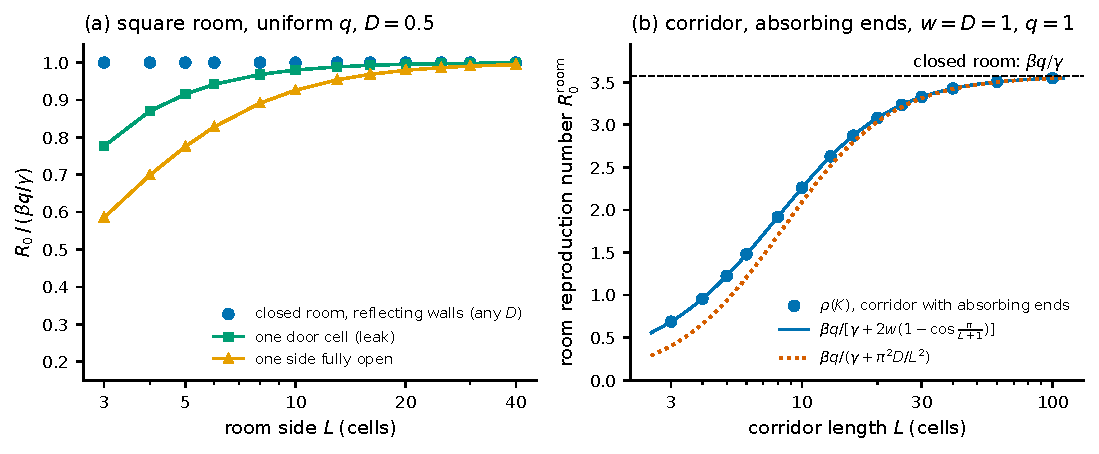
\includegraphics[width=\textwidth]{fig_room_size_leak_en}
  \caption{Room size and leaks in the mean-field model with uniform $q$ ($\beta q=0.5\perday$,
  $\gamma=0.14\perday$, same-cell kernel). (a) Ratio of the reproduction number to $\beta q/\gamma$ for
  $L\times L$ rooms with $D=0.5\cellday$: closed room with reflecting walls (circles; identical for every
  $D$), room with one door cell with exit rate $\kappa=D$ (squares) and room with one side fully open
  ($\kappa=D$ in each cell along that side; triangles). (b) Corridor of $L$ cells with absorbing ends, hop rate
  $w=D=1\perday$, $q=1$: $\Rroom=\srad(\ngm)$ computed numerically (circles), the closed form
  \eqref{M-s4_geometry:eq:corridor} (solid) and its continuum limit $\beta q/(\gamma+\pi^2D/L^2)$ (dotted); the
  dashed line is the closed-room value $\beta q/\gamma$. Numbers in Table~\ref{s4_geometry:tab:leak}.}
  % src: data/bsc_theory/fig2_room_size_data.json; drawn by code/plan_fig_theory.py
  \label{s4_geometry:fig:leak}
\end{figure}

\begin{proof}[Proof of Theorem~\ref{M-s4_geometry:thm:closed}]
  Since $\ker$ is row-stochastic, $\ker\one=\one$, so $\one^{\T}\Fm=\beta q_0\,\one^{\T}\ker^{\T}=\beta q_0\,\one^{\T}$.
  Since $\one^{\T}\gen=0$, $\one^{\T}\Vm=\gamma\one^{\T}$ and $\one^{\T}\Vm^{-1}=\gamma^{-1}\one^{\T}$. Hence
  $\one^{\T}\ngm=(\beta q_0/\gamma)\,\one^{\T}$: all column sums of $\ngm$, which are the offspring numbers
  $\noff(x)$ of \eqref{M-s3_r0:eq:offspring}, equal $\beta q_0/\gamma$. By (P4) there is $\wvec\ge0$, $\wvec\ne0$,
  with $\ngm\wvec=\srad(\ngm)\wvec$; then
  $\srad(\ngm)\,\one^{\T}\wvec=\one^{\T}\ngm\wvec=(\beta q_0/\gamma)\,\one^{\T}\wvec$ and $\one^{\T}\wvec>0$, so
  $\Rz=\beta q_0/\gamma$. Likewise $\one^{\T}\Jm=(\beta q_0-\gamma)\one^{\T}$. The matrix $\Jm^{\T}$ is Metzler
  and irreducible (because $\gen$ is, and $\Fm\ge0$) and has the positive eigenvector $\one$, so by (P1) the
  corresponding eigenvalue is $\sabs(\Jm^{\T})=\lamone$. The argument uses only the irreducibility of $\gen$
  and $\one^{\T}\gen=0$, neither of which depends on the size or shape of $\cells$, on the mobilities or on
  the hopping rule.
\end{proof}

\begin{proof}[Proof of Theorem~\ref{M-s4_geometry:thm:leaky}]
  (1) $\genk$ has the off-diagonal entries of $\gen$, so it is Metzler and irreducible. $\Vm_\kappa$ has
  non-positive off-diagonal entries and column sums $\gamma+\kappa_x>0$, so by (P5) it is a non-singular
  M-matrix, $\sabs(\genk-\gamma\Id)<0$ and
  $\Vm_\kappa^{-1}=\int_0^\infty\e^{-\gamma t}\e^{\genk t}\,\dd t>0$, where $(\e^{\genk t})_{yx}$ is the
  probability that a person who started in $x$ is still in the room, in cell $y$, at time $t$. These are the
  only properties of $\gen$ and $\Vm$ used in the proof of Theorem~\ref{M-s3_r0:thm:ngm}(a)--(c), which applies
  verbatim.

  (2) By (P1), $\sabs(\gen)=0$, because $\one^{\T}\gen=0$ with $\one>0$. (P3) with $A=\genk$ and
  $E=\diag\kappa$ gives $0=\sabs(\gen)>\sabs(\genk)$, and the same argument applied to $\kappa\le\kappa'$ gives
  the monotonicity. The function $f(v)=\sabs(\gen+\diag v)$ is convex with $f(0)=0$ and gradient $\stat$ at
  $v=0$ (P6; the Perron vectors of $\gen$ are $\stat$ and $\one$), so $f(v)\ge\sum_x\pi_xv_x$; $v=-\kappa$ gives
  $-\muk\ge-\sum_x\pi_x\kappa_x$. For the limit write $\mu(k)$ for $\muk$ with $\kappa=k\one_\Delta$ and
  $\Delta^c=\cells\setminus\Delta$. The principal submatrix of $\genk$ on $\Delta^c$ does not depend on $k$, so
  (P2) gives $\mu(k)\le\mu^{\mathrm{abs}}_\Delta$; being non-decreasing, $\mu(k)\uparrow\mu^*\le\mu^{\mathrm{abs}}_\Delta$.
  Let $\uvec_k\ge0$, $\one^{\T}\uvec_k=1$, be the Perron vector. Row $x\in\Delta$ of
  $(\gen-k\diag\one_\Delta)\uvec_k=-\mu(k)\uvec_k$ reads
  $u_k(x)=\sum_{y\ne x}M_{xy}u_k(y)/(k-\mu(k)-M_{xx})\to0$. Any limit point $\uvec^*$ of $(\uvec_k)$ therefore
  vanishes on $\Delta$, is non-negative and non-zero on $\Delta^c$ and satisfies
  $\gen[\Delta^c,\Delta^c]\uvec^*=-\mu^*\uvec^*$ there; hence $-\mu^*\le\sabs(\gen[\Delta^c,\Delta^c])$, that is
  $\mu^*\ge\mu^{\mathrm{abs}}_\Delta$.

  (3) $\Vm_\kappa\uvec_\kappa=(\gamma+\muk)\uvec_\kappa$, so the positive matrix $\Vm_\kappa^{-1}$ has the
  positive eigenvector $\uvec_\kappa$ with eigenvalue $1/(\gamma+\muk)$, which is its spectral radius by (P1)
  and (P4); and $\beta\Qm\Vm_\kappa^{-1}=\beta q_0\Vm_\kappa^{-1}$.

  (4) The upper bound follows from $0\le\beta\Qm\Vm_\kappa^{-1}\le\beta\qmax\Vm_\kappa^{-1}$, (P4) and (3). For
  the lower bound, $f_\kappa(v)=\sabs(\genk+\diag v)$ is convex with $f_\kappa(0)=-\muk$ and gradient $\nu$ at
  $v=0$ (P6), so $f_\kappa(v)\ge-\muk+\sum_x\nu_xv_x$. By (1), $f_\kappa(v)=0$ for
  $v=\beta\qvec/\Rroom-\gamma\one$, which gives $0\ge-\muk+\beta\langle q\rangle_\nu/\Rroom-\gamma$.
\end{proof}

\begin{proof}[Proof of Corollary~\ref{M-s4_geometry:cor:cases}]
  (a) $\genk=\gen-T^{-1}\Id$ has the Perron vectors $\stat$ and $\one$ of $\gen$, so $\muk=1/T$, $\nu=\stat$ and
  $\Vm_\kappa=(\gamma+1/T)\Id-\gen$; the expected number of infections is the identity
  $\sum_x\pi_x\noff(x)=\beta\qmean/\gamma$ of \eqref{M-s3_r0:eq:offspring} with $\gamma+1/T$ in place of
  $\gamma$. The form of $\Vm_\kappa$ does not involve the kernel, so for $\Fm=\beta\ker^{\T}\Qm$ the next-generation
  matrix is that of the closed room with $\gamma+1/T$ in place of $\gamma$, and Theorem~\ref{M-s4_geometry:thm:closed}
  gives the last statement. (b) $\genk=-w\,\mathbf{T}_L$, where
  $\mathbf{T}_L$ is the $L\times L$ tridiagonal matrix with $2$ on the diagonal and $-1$ beside it. Its
  eigenvalues are $2-2\cos(j\pi/(L+1))$ with eigenvectors $(\sin(j\pi x/(L+1)))_{x=1}^{L}$, $j=1,\dots,L$; the
  eigenvector for $j=1$ is positive, hence the Perron vector by (P1). Then apply
  Theorem~\ref{M-s4_geometry:thm:leaky}(3).
\end{proof}

\begin{remark}[Other kernels and a localised door]\label{s4_geometry:rem:kernels}
  With a localised door, parts (3) and (4) of Theorem~\ref{M-s4_geometry:thm:leaky} do not extend to other
  contact kernels ($\Rroom:=\srad(\beta\ker^{\T}\Qm\Vm_\kappa^{-1})$). Take three cells in a row, hop rate
  $1\perday$ between neighbours, a door with $\kappa=1\perday$ at one end ($\muk=0.198\perday$), $q\equiv1$,
  $\beta=0.5\perday$ and $\gamma=0.14\perday$, so that the formula of part (3) gives $1.479$. With $\ker$ uniform
  over a cell and its neighbours, $\Rroom=1.435$ ($-3.0\,\%$); with the rows of $\ker$ equal to $(0,0,1)$,
  $(0,1,0)$, $(0,0,1)$ and the door at cell~1 (the cell whose contacts land in cell~3), $\Rroom=1.640$, which
exceeds the upper bound of part (4) by $10.9\,\%$ (with the door at cell~3 it is $1.127$, within the bounds). The lower bound
  fails by continuity: as $\kappa\to0$, $\Rroom\to\Rz$ and the lower bound tends to $\beta\qmean/\gamma$,
  which the kernel of Proposition~\ref{M-s3_r0:prop:kernel}(iv) violates. In that example with hop rate
  $0.01\perday$ and a door with $\kappa=0.01\perday$ at one end, $\Rroom=1.845$ against a lower bound of $2.292$.
\end{remark}
% src: data/s4_geometry_leak_kernels.json (a_uniform_q_neighbour_kernel_end_door: R_room 1.4348, formula 1.4790, mu_leak 0.19806, -2.99 %; b_uniform_q_skew_kernel_end_door: R_room 1.6403, excess 10.91 %; c_prop_3_15_iv_kernel_q101_D0_0.01."end door|kappa=0.01": R_room 1.8447, lower_bound 2.2915; bound fails at every kappa from 1e-4 to 1); door position of the skewed kernel: door at cell 1 gives 1.6403, at cell 3 1.1267 (recomputed with the rows of P and the generator stated in the remark)

For heterogeneous $q$ and a localised door the substitution $\gamma\to\gamma+\muk$ is not exact, and only
the bounds of Theorem~\ref{M-s4_geometry:thm:leaky}(4) hold. In the office scene with one door cell at the end
of a corridor arm, $\kappa=1\perday$ and $\Dz=1\cellday$ give $\Rroom=5.107$ where the substitution gives
$5.060$ ($\muk=0.00137\perday$); with $\kappa=100\perday$ and $\Dz=10$, $\Rroom=4.220$ where the substitution
gives $4.133$, which is below the lower bound $\beta\langle q\rangle_\nu/(\gamma+\muk)=4.139$ (upper bound
$4.730$). A door at the end of the corridor removes people from a low-$q$ zone, so the walk conditioned to
stay is weighted towards higher $q$ ($\langle q\rangle_\nu=1.306$ and $1.313$ in the two cases, against
$\langle q\rangle=1.300$) than under a uniform leak at the same rate, for which the substitution is exact
(Corollary~\ref{M-s4_geometry:cor:cases}a).
% src: data/s4_geometry_barriers_leak.json: B_leak_heterogeneous_q/cases/"D0=1|kappa=1" (R_room 5.1072,
%      R_substitution 5.0598, mu_leak 0.00137), "D0=10|kappa=100" (R_room 4.2201, R_substitution 4.1331, lower_bound
%      4.1386, upper_bound 4.7297; q_mean_nu 1.3060, 1.3125); uniform_leak_T_8h (substitution exact to 1e-15); random_nonreversible (1500
%      instances: bounds never violated; the substitution lies below the lower bound in 455)

The lattice leak rate of the corridor of Corollary~\ref{M-s4_geometry:cor:cases}(b) is $0.53$, $0.86$ and $0.98$ of its
continuum limit $\pi^2D/L^2$ at $L=3$, $13$ and $100$ (Fig.~\ref{s4_geometry:fig:leak}b).
% src: data/s4_geometry_checks.json: A_room_size_and_leaks/corridor_w1_q1/{3,13,100}/ratio_to_continuum
%      (0.534, 0.859, 0.980); same values in data/checks/theory.json: corridor_absorbing_ends (0.53, 0.86, 0.98;
%      notes/VERIFICATION.md: Section 4.1, theory, item 9)

\begin{observation}[One-door square room]\label{s4_geometry:obs:door}
  For an $L\times L$ room with hop rate $D$ and one absorbing door cell in the middle of a boundary row, the
  leak rate is
  $\mu^{\mathrm{abs}}\approx\pi D/\bigl(L^2\ln(L/c)\bigr)$ with a fitted $c$ that rises from $0.82$ at $L=8$ to
  $0.91$ at $L=128$ and has not converged. For a door cell with finite exit rate $\kappa=D$,
  $1/\muk\approx1/\mu^{\mathrm{abs}}+1/\langle\kappa\rangle_\pi$ (search time plus exit time), with a relative
  error in $\muk$ that falls from $1.5\,\%$ at $L=8$ to $0.3\,\%$ at $L=128$.
\end{observation}
% src: data/bsc_theory/worked_examples.json: E6_room_size/narrow_escape (c_fit 0.822, 0.864, 0.885,
%      0.898, 0.907; series_rel_err -1.51, -0.90, -0.58, -0.39, -0.28 %); reproduced with separately written code in
%      code/bsc_theory/verify/v2_examples.log and data/s4_geometry_checks.json: A_room_size_and_leaks/one_door_D1
The logarithm is that of the two-dimensional narrow-escape law \citep{schuss2007narrow}; we have not proved
either statement.

\begin{table}[tbp]
  \centering
  \caption{Square rooms of side $L$ cells with uniform $q$ and $D=0.5\cellday$ ($\gamma=0.14\perday$): leak
  rate $\muk$ (per day) and ratio of the reproduction number to $\beta q/\gamma$, which by
  Theorem~\ref{M-s4_geometry:thm:leaky}(3) equals $\gamma/(\gamma+\muk)$. The door cell lies in the middle of
  one side; `one side open' means $\kappa=D$ in every cell along one side.}
  \label{s4_geometry:tab:leak}
  \small
  \begin{tabular}{@{}rccccc@{}}
    \toprule
        & closed room & \multicolumn{2}{c}{one door cell ($\kappa=D$)} & \multicolumn{2}{c}{one side open} \\
    \cmidrule(lr){2-2}\cmidrule(lr){3-4}\cmidrule(l){5-6}
    $L$ & ratio & $\muk$ & ratio & $\muk$ & ratio \\
    \midrule
    3   & 1.000 & 0.0403  & 0.777 & 0.0990  & 0.586 \\
    13  & 1.000 & 0.00160 & 0.989 & 0.00676 & 0.954 \\
    20  & 1.000 & 0.00063 & 0.996 & 0.00293 & 0.979 \\
    40  & 1.000 & 0.00014 & 0.999 & 0.00075 & 0.995 \\
    \bottomrule
  \end{tabular}
  % src: data/bsc_theory/worked_examples.json: E6_room_size/{3,13,20,40}
  %      (reflecting, one_door_mu, one_door_ratio, open_wall_mu, open_wall_ratio);
  %      recomputed with separately written code in data/s4_geometry_checks.json: A_room_size_and_leaks/square_rooms_D0.5
  %      (largest deviation 3e-6). Note: open_wall_ratio at L = 20 is 0.97947, i.e. 0.979.
\end{table}

Table~\ref{s4_geometry:tab:leak} gives the leak rates of square rooms. They are small ($\muk\le0.1\perday$, residence times $1/\muk$ from
$10$ days to $19$ years) only because $D=0.5\cellday$. For a fixed geometry and a door whose exit rate is itself
a hop rate ($\kappa=D$, as in Table~\ref{s4_geometry:tab:leak}) $\muk$ is proportional to the mobility scale, so at
$D=2.4\times10^{3}\cellday$ (Section~\ref{M-s2_model:sec:regime}) the same residence times
would lie between $3$ minutes and $1.5$ days. A door with a fixed exit rate $\kappa$ behaves differently: its
leak rate grows with mobility but stays below $\langle\kappa\rangle_\pi$
(Theorem~\ref{M-s4_geometry:thm:leaky}(2)). In the office with one door cell at the end of a corridor arm and
$\kappa=1\perday$, $\muk=0.00137$, $0.00356$, $0.00419$ and $0.00427\perday$ at $\Dz=1$, $10$, $100$ and
$2{,}400$, against the cap $1/234=0.00427\perday$, and $\Rroom/\Rz=0.99998$, $0.977$, $0.971$ and $0.970$; with
$\kappa$ equal to the hop rate of the door cell, $\muk=0.00152\,\Dz$ and $\Rroom/\Rz$ falls to $0.916$,
$0.483$ and $0.037$ at $\Dz=10$, $100$ and $2{,}400$. For applications the dwell time $T$ should therefore be an
input, as in Corollary~\ref{M-s4_geometry:cor:cases}(a), not the output of a random walk towards a door.
% src: data/s4_geometry_checks.json: A_room_size_and_leaks/residence_days_range_D0.5 (10.1 d, 7041 d = 19.3 yr),
%      max_mu_D0.5 (0.099), residence_range_at_D2400 (3.0 min, 1.47 d); data/s4_geometry_leak_kernels.json
%      (d_office_door_against_mobility: fixed_kappa_1 mu_leak 0.00137, 0.00356, 0.00419, 0.00427, R_room_over_R0 0.99998, 0.977, 0.971, 0.970;
%      kappa_mean_pi_for_kappa_1 0.004274 (234 cells); kappa_equal_door_hop_rate mu_over_D0 0.001521, R_room_over_R0 0.916, 0.483, 0.037)

\subsection{Hotspot maps}\label{appS_geometry:sec:hotspot}

\begin{proof}[Proof of Theorem~\ref{M-s4_geometry:thm:hotspots}]
  (i) By (P1), $\lamone$ is a simple eigenvalue of $\Jm$ with spectral projector
  $\uvec\lvec^{\T}/(\lvec^{\T}\uvec)$. For $c>\max_x|J_{xx}|$ the matrix $\Jm+c\Id$ is non-negative and
  irreducible with a positive diagonal, hence primitive \citep{berman1994nonnegative}, so every other
  eigenvalue $\lambda$ of $\Jm$
  satisfies $|\lambda+c|<\lamone+c$ and thus $\operatorname{Re}\lambda<\lamone$: $\delta>0$. On the
  complementary invariant subspace $\e^{\Jm t}$ is $O(\e^{(\lamone-\delta')t})$ for every $\delta'<\delta$, and
  for $\delta'=\delta$ when $\Jm$ is diagonalisable; for reversible movement $\Jm$ is similar to the symmetric
  matrix $\Pi^{-1/2}\Jm\,\Pi^{1/2}$. If $q\equiv q_0$, $\Jm\stat=(\beta q_0-\gamma)\stat$ and $\stat>0$, so
  $\uvec=\stat$ by (P1). Conversely, $\Jm\stat=\lamone\stat$ reads $(\beta q_x-\gamma)\pi_x=\lamone\pi_x$ for all
  $x$, so $q$ is constant.

  (ii) $\ngm=\beta\Qm\Vm^{-1}>0$ entrywise, so $\ngm$ is primitive and $\ngm^{g}/\Rz^{g}\to\wvec\zvec^{\T}/(\zvec^{\T}\wvec)$.
  Put $\xi=\Vm^{-1}\wvec>0$; then $\beta\Qm\xi=\ngm\wvec=\Rz\wvec=\Rz\Vm\xi$, so $\xi$ solves the stated
  problem and $\wvec=\beta\Qm\xi/\Rz$. Any other solution $\xi'$ gives an eigenvector $\Vm\xi'$ of $\ngm$ for
  the simple eigenvalue $\Rz$, hence $\xi'\propto\xi$. Finally $\Vm\stat=\gamma\stat$ gives
  $\ngm\stat=\beta\Qm\stat/\gamma$.

  (iii) For a simple eigenvalue \citep{horn2013matrix},
  $\partial\Rz/\partial q_x=\zvec^{\T}(\partial\ngm/\partial q_x)\wvec/(\zvec^{\T}\wvec)$ with
  $\partial\ngm/\partial q_x=\beta\boldsymbol{\delta}_x\boldsymbol{\delta}_x^{\T}\Vm^{-1}$, so that
  $\zvec^{\T}(\partial\ngm/\partial q_x)\wvec=\beta z_x\xi_x=\Rz z_xw_x/q_x$. This is the formula for $e_x$;
  the $e_x$ are positive and sum to one. Next, let $\mathbf{A}=\gen+\beta\Qm/\Rz-\gamma\Id$. Then
  $\mathbf{A}\xi=0$ and, multiplying $\zvec^{\T}\ngm=\Rz\zvec^{\T}$ by $\Vm$ from the right,
  $\zvec^{\T}\mathbf{A}=0$: $\xi$ and $\zvec$ are the right and left Perron vectors of $\mathbf{A}$, and
  \begin{equation}\label{s4_geometry:eq:theta}
     e_x=\frac{q_x\theta_x}{\sum_yq_y\theta_y},\qquad \theta_x=\frac{z_x\xi_x}{\zvec^{\T}\xi} ,
  \end{equation}
  where by (P6) $\theta$ is the gradient of $f(v)=\sabs(\gen+\diag v)$ at $v_0=\beta\qvec/\Rz-\gamma\one$.
  Detailed balance reads $\gen\Pi=\Pi\gen^{\T}$, so $\mathbf{A}^{\T}=\Pi^{-1}\mathbf{A}\Pi$ and
  $\mathbf{A}^{\T}\Pi^{-1}\xi=0$: $\zvec\propto\Pi^{-1}\xi$ and $e_x\propto q_x\xi_x^2/\pi_x$.

  (iv) \emph{Fast mixing.} $\stat\one^{\T}$ is the spectral projector of $\genz$ for its simple eigenvalue $0$,
  and $\genz$ is invertible on the complementary invariant subspace, so
  $\Vm^{-1}=\gamma^{-1}\stat\one^{\T}+\Dz^{-1}(\gamma/\Dz-\genz)^{-1}(\Id-\stat\one^{\T})\to\gamma^{-1}\stat\one^{\T}$
  and $\ngm\to(\beta/\gamma)\Qm\stat\one^{\T}$. The limit has the simple eigenvalue $\beta\qmean/\gamma$ with
  right eigenvector $\Qm\stat$ and left eigenvector $\one$; the eigenvectors of a simple eigenvalue depend
  continuously on the matrix, which gives the limits of $\wvec$ and of $e_x=z_xw_x/(\zvec^{\T}\wvec)$. In the
  same way $\Jm/\Dz\to\genz$, whose Perron vector is $\stat$.

  \emph{Slow mixing.} As $\Dz\to0$, $\ngm\to\beta\Qm/\gamma$, $\Jm\to\beta\Qm-\gamma\Id$, $\Rz\to\beta\qmax/\gamma$ and
  $\lamone\to\beta\qmax-\gamma$. The vectors $\uvec$ lie in the unit simplex, and every limit point $\uvec^*$
  satisfies $(\beta q_x-\gamma)u^*_x=(\beta\qmax-\gamma)u^*_x$, so it vanishes outside $Z$; the same argument
  applies to $\wvec$. The limiting eigenvalue is degenerate when $Z$ has several cells, so for $\evec$ we use
  \eqref{s4_geometry:eq:theta} and convexity instead. Because $\one^{\T}(\gen+\diag v)\le(\max_yv_y)\one^{\T}$,
  pairing with a non-negative right Perron vector gives $f(v)\le\max_yv_y$; and by (P2),
  $f(v)\ge\max_y(v_y+M_{yy})\ge\max_yv_y-\Dz c$ with $c=\max_y|(\genz)_{yy}|$. Let
  $m=\max_y(v_0)_y=\beta\qmax/\Rz-\gamma$. Since $f(v_0)=0$ by Theorem~\ref{M-s3_r0:thm:ngm}(b), $0\le m\le\Dz c$.
  For $x\notin Z$ and $t=\beta(\qmax-q_x)/\Rz>0$ the vector $v_0+t\boldsymbol{\delta}_x$ still has maximum $m$,
  so the tangent inequality for the convex function $f$ gives
  $t\,\theta_x\le f(v_0+t\boldsymbol{\delta}_x)-f(v_0)\le m\le\Dz c$. As $\Rz\le\beta\qmax/\gamma$,
  $t\ge\gamma(1-q_x/\qmax)$, hence $\theta_x\le\Dz c/\bigl(\gamma(1-q_x/\qmax)\bigr)$, and
  $e_x\le(q_x/\qmin)\,\theta_x\to0$.
\end{proof}

\begin{remark}[Transients]\label{s4_geometry:rem:transient}
  The prevalence map $\uvec$ is reached after a time of order $1/\delta$, whereas the exponential phase started
  by one index case among $\Npop$ people lasts about $\ln\Npop/\lamone$. When $1/\delta$ is not small compared
  with $\ln\Npop/\lamone$, the early pattern depends on where the index case sits and is given by the
  seed-specific transient $\e^{\Jm t}I(0)$. The part of an outbreak that has not yet left a zone $Z$ with
  uniform $q$ evolves by $\e^{\Jm[Z,Z]t}$ and grows at the zone rate
  $\sabs(\Jm[Z,Z])=\beta q_Z-\gamma-\muZ\le\lamone$ (cf.\ Proposition~\ref{M-s3_r0:prop:zone}). The threshold
  statement of Theorem~\ref{M-s3_r0:thm:ngm} is unaffected.
\end{remark}

In the office scene at $\Dz=1\cellday$ (Fig.~\ref{M-s4_geometry:fig:hotspots}),
the expected number of secondary cases of an index case, $\noff(x)$, ranges from $3.995$ to $5.335$ over the
starting cell.
% src: data/plan_theory_checks.json: office/D0=1/{offspring_min,offspring_max}
The elasticity share of the meeting room falls to $20.8\,\%$ at $\Dz=10$ and $13.4\,\%$ at $\Dz=100\cellday$,
close to its limit $q_x\pi_x/\qmean$ summed over the room, $12.8\,\%$; the prevalence share falls to
$50.3\,\%$ and $12.4\,\%$.
% src: data/plan_theory_checks.json: office/D0=10, office/D0=100 (elasticity_share/M, prevalence_share_u/M);
%      limit: data/s4_geometry_checks.json: C_office_hotspot_identities/meeting_room_share_limit_e_and_w
The first generation of a uniformly placed index case puts $12.8\,\%$ of its infections in the meeting room
at every mobility (Theorem~\ref{M-s4_geometry:thm:hotspots}(ii)), against $79.2\,\%$ asymptotically at
$\Dz=1\cellday$.
% src: data/plan_theory_checks.json: office/D0=1/first_generation_share_uniform_index/M

The transient of Remark~\ref{s4_geometry:rem:transient} matters in this scene. At $\Dz=1\cellday$ the gap is
$\delta=0.061\perday$ ($1/\delta=16$ days), while $\lamone=0.602\perday$ and $\ln100/\lamone=7.6$ days. In the
linearised dynamics, a point seed at a workstation far from the meeting room grows at $0.553\perday$ while
the total rises from $10^2$ to $10^4$ times the seed, between the workstation-zone rate $0.531\perday$ and
$\lamone$, and its spatial distribution is then still at total-variation distance $0.996$ from $\uvec$; a seed
in the meeting room grows at $0.605\perday$ and is at distance $0.026$.
% src: data/plan_theory_checks.json: office/D0=1/gap, office/transient_linear/{D0=1|far_workstation,
%      D0=1|meeting_room}/{fitted_rate_1e2_to_1e4,tv_to_u};
% src: data/s4_geometry_checks.json: D_derived/{mixing_time_1_over_gap_days,
%      linear_phase_ln100_over_lambda1_days,workstation_zone_growth_rate}
At $\Dz=100\cellday$ ($\delta=0.537\perday$) the distance is below $10^{-4}$ from either seed.
% src: data/plan_theory_checks.json: office/transient_linear/D0=100|* (1.8e-5, 5.9e-5), office/D0=100/gap

\subsection{Worked examples on the office scene}\label{appS_geometry:sec:examples}\label{s4_geometry:sec:examplesdetail}

\begin{figure}[tbp]
  \centering
  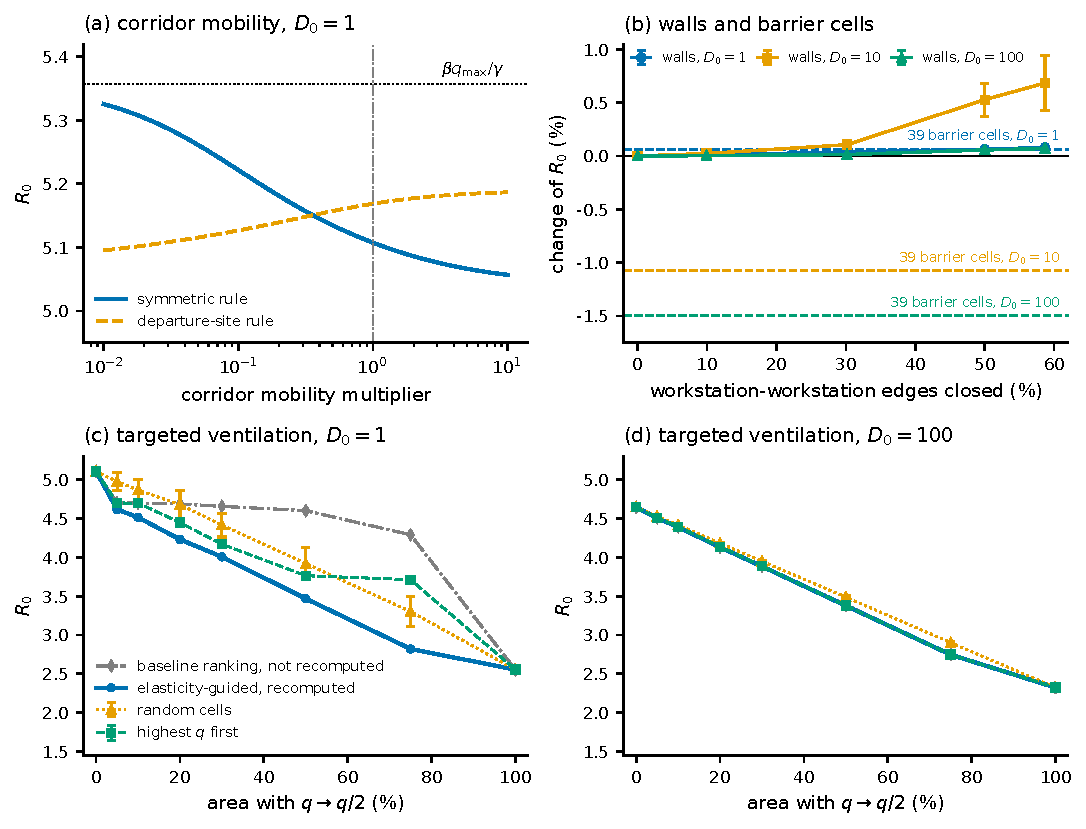
\includegraphics[width=\textwidth]{fig_s4_interventions_en}
  \caption{Mean-field $\Rz$ of the office scene under interventions
  ($\beta=0.5\perday$, $\gamma=0.14\perday$, same-cell kernel). (a) Corridor mobility multiplied by a factor,
  for the symmetric rule \eqref{M-s2_model:eq:hop} and for a departure-site rule; dotted line: upper bound $\beta\qmax/\gamma$. (b) Change of $\Rz$ at $\Dz=1$, $10$ and
  $100\cellday$ when walls close a fraction of the $242$ edges between workstation cells (symbols: mean and
  standard deviation over $20$ random draws that keep the room connected; the last point closes as many edges
  as connectivity allows), and when $39$ workstation cells are turned into barrier cells (dashed lines: means
  over $40$ draws). Walls never lower $\Rz$ (Theorem~\ref{M-s3_r0:thm:edges}); barrier cells, which remove
  floor with $q$ above the mean, lower it at $\Dz=10$ and $100$. (c), (d) Targeted ventilation, $q\to q/2$ on a
  fraction of the floor, at $\Dz=1$ and $\Dz=100\cellday$: cells chosen by the elasticity map recomputed after
  every six cells, by the baseline elasticity ranking without recomputation, by highest $q$ first (ties
  broken at random) and at random (means and standard deviations over $30$ draws).}
  % src: data/plan_theory_checks.json (office/targeted_ventilation), data/plan_corridor_sweep.json
  %      and data/s4_geometry_barriers_leak.json (A_partitions; panel b); drawn by
  %      code/s4_geometry_fig_interventions.py
  \label{s4_geometry:fig:interventions}
\end{figure}

\begin{table}[tbp]
  \centering
  \caption{Worked examples on the office scene (mean-field model, same-cell kernel; baseline $\Rz=5.107$,
  $4.676$ and $4.646$ at $\Dz=1$, $10$ and $100\cellday$; bounds $4.643\le\Rz\le5.357$): interventions on
  movement (walls: mean over $20$ random draws; barrier cells: mean over $40$ draws, which lowers the
  well-mixed value $\beta\langle q\rangle/\gamma$ of the remaining floor from $4.643$ to $4.571$) and uniform
  measures. Targeted ventilation is in Table~\ref{s4_geometry:tab:targeting}.}
  % src: data/plan_theory_checks.json: office/D0=1/R0, office/D0=100/R0, office/lower_bound, office/upper_bound
  \label{s4_geometry:tab:office}
  \small
  \setlength{\tabcolsep}{4.5pt}
  \begin{tabular}{@{}lcccc@{}}
    \toprule
     & $\Rz$ at $\Dz=1$ & \multicolumn{3}{c}{change of $\Rz$ (\%) at $\Dz=$} \\
    \cmidrule(l){3-5}
    Intervention & & 1 & 10 & 100 \\
    \midrule
    corridor mobility $\times0.3$ & 5.159 & $+1.0$ & & \\
    corridor mobility $\times0.1$ & 5.222 & $+2.2$ & & \\
    corridor mobility $\times0.01$ & 5.325 & $+4.3$ & & \\
    walls on 24 of the 242 workstation--workstation edges & 5.1077 & $+0.009$ & $+0.023$ & $+0.003$ \\
    walls on 73 edges & 5.1092 & $+0.038$ & $+0.105$ & $+0.013$ \\
    walls on 121 edges & 5.1105 & $+0.064$ & $+0.53$ & $+0.056$ \\
    walls on 142 edges (as many as keep the room connected) & 5.1114 & $+0.080$ & $+0.68$ & $+0.070$ \\
    39 workstation cells made barrier cells & 5.1106 & $+0.065$ & $-1.07$ & $-1.49$ \\
    $q\to q/2$ in every cell & 2.554 & \multicolumn{3}{c}{$\times0.5$ (exact)} \\
    $\beta\to0.3\beta$ and $q\to q/2$ in every cell & 0.766 & \multicolumn{3}{c}{$\times0.15$ (exact)} \\
    \bottomrule
  \end{tabular}
  % src: data/plan_theory_checks.json: office/corridor_multiplier_symmetric;
  %      data/s4_geometry_barriers_leak.json: A_partitions/walls/{walls_10pct,walls_30pct,walls_50pct,walls_100pct}
  %      and A_partitions/barrier_cells_39_workstations (D0=1, D0=10, D0=100: mean, change_pct; same random draws as
  %      plan_theory_checks.json: office/partitions, whose D0 = 1 means are reproduced to 1e-9);
  %      uniform scalings: data/s4_geometry_checks.json: D_derived

\end{table}

\begin{table}[tbp]
  \centering
  \caption{Targeted ventilation in the office scene (mean-field model, same-cell kernel): $\Rz$ after
  $q\to q/2$ on a fraction of the floor, at equal treated area for four placement rules (as in
  Fig.~\ref{s4_geometry:fig:interventions}c,d; mean $\pm$ standard deviation over $30$ draws). Baseline
  $\Rz=5.107$ at $\Dz=1$ and $4.646$ at $\Dz=100\cellday$.}
  \label{s4_geometry:tab:targeting}
  \footnotesize
  \setlength{\tabcolsep}{5pt}
  \begin{tabular}{@{}rrcccc@{}}
    \toprule
    $\Dz$ & treated area (cells) & recomputed elasticity & highest $q$ first & random cells & baseline ranking, \\
          &                      &                       &                   &              & not recomputed \\
    \midrule
    1   & 10\pct{} (23)  & 4.515 & $4.699\pm0.0002$ & $4.867\pm0.131$ & 4.700 \\
    1   & 20\,\% (47)  & 4.231 & $4.449\pm0.041$ & $4.680\pm0.182$ & 4.688 \\
    1   & 50\,\% (117) & 3.468 & $3.764\pm0.019$ & $3.921\pm0.209$ & 4.602 \\
    1   & 75\,\% (176) & 2.821 & $3.712\pm0.003$ & $3.302\pm0.196$ & 4.291 \\
    1   & 100\,\% (234) & 2.554 & 2.554 & 2.554 & 2.554 \\
    \addlinespace
    100 & 10\,\% (23)  & 4.390 & $4.395\pm0.0003$ & $4.416\pm0.009$ & 4.396 \\
    100 & 20\,\% (47)  & 4.130 & $4.137\pm0.001$ & $4.182\pm0.014$ & 4.135 \\
    100 & 50\,\% (117) & 3.377 & $3.379\pm0.001$ & $3.487\pm0.015$ & 3.388 \\
    100 & 75\,\% (176) & 2.746 & $2.747\pm0.0003$ & $2.900\pm0.011$ & 2.750 \\
    100 & 100\,\% (234) & 2.323 & 2.323 & 2.323 & 2.323 \\
    \bottomrule
  \end{tabular}
  % src: data/plan_theory_checks.json: office/targeted_ventilation/{D0=1,D0=100}/rows
  %      (adaptive, highest_q_mean +- highest_q_sd, random_mean +- random_sd, one_shot)
\end{table}

Table~\ref{s4_geometry:tab:office} and Fig.~\ref{s4_geometry:fig:interventions} give what the mean-field model says
about interventions on the office scene.

\emph{Slower corridors raise $\Rz$.} Multiplying the corridor mobility by $0.1$ moves $\Rz$ from $5.107$ to
$5.222$, and by $0.01$ to $5.325$, as Theorem~\ref{M-s3_r0:thm:edges} requires: less movement means less mixing
between high-$q$ and low-$q$ cells. Under a departure-site rule (hop rate $D_x$ from cell $x$) the same change
lowers $\Rz$ ($5.169$, $5.127$ and $5.095$ at multipliers $1$, $0.1$ and $0.01$), but only because people then
accumulate in the slowed corridor, where $q$ is lowest ($\qmean$ falls from $1.379$ to $1.218$ and $0.911$).
That is an occupancy effect in a different model.
% src: data/plan_theory_checks.json: office/corridor_multiplier_symmetric,
%      office/corridor_multiplier_departure_reading (R0, q_mean_pi)

\emph{Walls cannot lower $\Rz$; barrier cells change the mean of $q$.} Two kinds of partition
must be kept apart. A wall closes edges and leaves the set of cells unchanged, so
Theorem~\ref{M-s3_r0:thm:edges} applies: closing between $10\pct$ of the workstation--workstation edges and
as many as connectivity allows raises $\Rz$ by $0.009\pct$ to $0.080\pct$ at $\Dz=1$, by $0.02\pct$ to
$0.68\pct$ at $\Dz=10$ and by $0.003\pct$ to $0.070\pct$ at $\Dz=100\cellday$, and none of the $80$ draws
lies below the baseline at any of the three mobilities. A barrier cell removes floor, and with it its $q$,
which the theorem does not cover. Turning $39$ workstation cells ($q=1.4$, above the mean $1.30$) into
barriers lowers the well-mixed value $\beta\langle q\rangle/\gamma$ of the remaining floor from $4.643$ to
$4.571$ ($-1.5\pct$). At $\Dz=1$, where $\Rz$ is pinned by the meeting room, the net change is $+0.065\pct$
(all $40$ draws above the baseline); at $\Dz=10$ and $100$ it is $-1.07\pct$ and $-1.49\pct$ (all $40$
draws below). These are numerical results for this floor plan, not consequences of a theorem.
% src: data/s4_geometry_barriers_leak.json: A_partitions/walls/*/D0=*/{change_pct,n_below_baseline} (0 in all
%      12 sets of 20 draws; 4 x 20 = 80 draws per mobility), A_partitions/barrier_cells_39_workstations
%      (wellmixed_after 4.5714, wellmixed_change_pct -1.54; D0=1: +0.065, 40 above; D0=10: -1.07, 40 below;
%      D0=100: -1.49, 40 below)

\emph{Targeted ventilation helps at low mobility, if the map is recomputed.} Here ventilation is an input: $q$
is halved by assumption on the treated cells (Fig.~\ref{s4_geometry:fig:interventions}c,d; numbers in
Table~\ref{s4_geometry:tab:targeting}). At $\Dz=1\cellday$ and equal treated area, choosing cells by the
elasticity map and recomputing it after every six cells gives an $\Rz$ that is lower than for random
placement by $0.35$ to $0.48$ between $5\pct$ and $75\pct$ treated area, and lower than for `highest $q$
first' by $0.18$ at $10\pct$ and $0.30$ at $50\pct$.
% src: data/s4_geometry_checks.json: D_derived/targeted_ventilation/D0=1/*/gain_recomputed_vs_random
%      (0.359, 0.352, 0.449, 0.409, 0.453, 0.482); Table rows for the differences to highest-q (4.699-4.515, 3.764-3.468)
The recomputation is essential, because the hotspot moves once the leading zone has been treated: a ranking
by the baseline elasticity that is not recomputed is no better than random placement from $20\pct$ treated
area on ($4.688$ against $4.680\pm0.182$) and clearly worse at $50\pct$ ($4.602$ against $3.921\pm0.209$).
% src: data/plan_theory_checks.json: office/targeted_ventilation/D0=1/rows (one_shot, random_mean, random_sd);
%      data/s4_geometry_checks.json: C_office_hotspot_identities/targeting_explanations_D0=1
At $\Dz=100\cellday$ the four rules differ by at most $0.11$ up to $50\pct$ treated area: in a well-mixed room
$e_x=q_x\pi_x/\qmean$ and targeting reduces to treating the cells with the largest $q$. For discrete
individuals at $\Dz=1\cellday$ the placement makes no measurable difference
(Section~\ref{M-s6_scenes:sec:interventions}).
% src: data/s4_geometry_checks.json: D_derived/targeted_ventilation/D0=100/*/spread (max 0.110 up to 50 %; 0.154 at 75 %)
% src: data/bsc_sim/08_interventions.json: office|D0=1|{hotspot,coldspot,pair-level hotspot} ventilation
%      (25 % of cells)|FD: R1_pair_uniform 2.075 / 2.090 / 2.062

\emph{Uniform measures scale $\Rz$ exactly.} Because $\ngm=\beta\Qm\Vm^{-1}$, multiplying $\beta$ by
$s_\beta$ and every $q_x$ by $s_q$ multiplies $\Rz$ by $s_\beta s_q$ for every geometry and mobility. Halving $q$ everywhere gives
$2.554$; a mask factor $\beta\to0.3\beta$ together with it gives $0.15\times5.107=0.766$. The product is
plain proportionality and involves no interaction between the two measures.
% src: data/plan_theory_checks.json: office/targeted_ventilation/D0=1/rows[fraction=1.0]/adaptive (2.5536);
%      data/s4_geometry_checks.json: D_derived/{uniform_q_half,uniform_mask0.3_and_q_half}

% supp_pair.tex -- Supplementary Section S4: pair-level theory; proofs, tables and a remark on the normalisation.
% Paths in "% src:" comments are relative to the repository root.
% Numbers: data/s5_pair_checks.json, data/s5_pair_tables.tex, data/bsc_sim/02_*.json.
\section{Pair-level theory: proofs and further results}\label{appS_pair:sec}

This section proves the statements of Section~\ref{M-s5_pair:sec} of the main text and gives the tables behind its
figures. Movement follows the symmetric rule \eqref{M-s2_model:eq:hop}, and (P1)--(P6) are the facts of
Lemma~\ref{s3_r0:lem:facts}.

\subsection{Proofs}

\begin{proof}[Proof of Proposition~\ref{M-s5_pair:prop:pair}]
Write $z=(x,y)$, let $r(z\to z')=\mathcal{M}_{z'z}$ ($z'\ne z$) be the hop rates of the pair chain,
$r(z)=\sum_{z'}r(z\to z')$, and $u=\one-p$. From state $z$ three kinds of independent exponential clocks
compete: recovery (rate $\gamma$), infection (rate $h(z)$) and a hop to $z'$ (rate $r(z\to z')$). If recovery
rings first the person escapes; if infection rings first it does not; if a hop to $z'$ rings first, the
Markov property and the lack of memory of $\tau$ give the escape probability $u(z')$. Hence
\[
  \bigl(\gamma+h(z)+r(z)\bigr)\,u(z)=\gamma+\sum_{z'}r(z\to z')\,u(z') ,
\]
which is $(\gamma\Id+\mathbf{H}-\mathcal{M}^{\T})u=\gamma\one$, because
$(\mathcal{M}^{\T}u)(z)=\sum_{z'}r(z\to z')\bigl(u(z')-u(z)\bigr)$. The matrix
$A=\gamma\Id+\mathbf{H}-\mathcal{M}^{\T}$ has non-positive off-diagonal entries and row sums
$\gamma+h(z)\ge\gamma>0$; by (P5) of Lemma~\ref{s3_r0:lem:facts} applied to $A^{\T}$ it is non-singular with
$A^{-1}\ge0$, so $u=\gamma A^{-1}\one$.
\end{proof}

The matrix $\ngmone$ is obtained from $\ncell$ further
solves: by the same first-step argument, the probability that the pair started at $(x,y)$ ends with an
infection while the susceptible is in cell $z$ is $w_z=A^{-1}b_z$ with $b_z(x',y')=h(x',y')\,\mathbf{1}\{y'=z\}$,
and $(K_1)_{zx}=\rhobar\sum_yw_z(x,y)$.

\begin{proof}[Proof of Proposition~\ref{M-s5_pair:prop:saturation}]
Let $T_{\mathrm{i}}$ be the infection time of the given person. Conditionally on the path of the pair and on
$\tau$, $T_{\mathrm{i}}$ has hazard $h(Z_t)$ on $[0,\tau)$, so that
\begin{align*}
  \Prob_{(x,y)}(T_{\mathrm{i}}<\tau,\,Y_{T_{\mathrm{i}}}=z)&=\int_0^\infty \e^{-\gamma t}\,
  \Exp_{(x,y)}\Bigl[h(X_t,z)\,\mathbf{1}\{Y_t=z\}\,\e^{-\int_0^th(Z_s)\,\dd s}\Bigr]\dd t\\
  &\le\int_0^\infty \e^{-\gamma t}\sum_{x'}P_t(x'\,|\,x)\,h(x',z)\,P_t(z\,|\,y)\,\dd t ,
\end{align*}
where the two walkers are independent. Because $\gen$ is symmetric, $\sum_yP_t(z\,|\,y)=1$. Summing over $y$
and multiplying by $(\Npop-1)/\ncell=\rhobar$,
\[
  (K_1)_{zx}\le\beta\sum_{x'}P_{x'z}\,q_{x'}\int_0^\infty \e^{-\gamma t}P_t(x'\,|\,x)\,\dd t=K_{zx}
\]
by Theorem~\ref{M-s3_r0:thm:ngm}(a). On the event $\{h(Z_t)>0\}$ the pair has almost surely been in its
current state for a positive time, so the discarded factor is smaller than one there and the inequality is
strict wherever $K_{zx}>0$. Column sums give $\Rone(x)<\noff(x)$ (recall $\noff(x)>0$); the uniform average and
eq.~\eqref{M-s3_r0:eq:offspring} give $\Ronebar<\beta\langle q\rangle/\gamma$; and (P4) of
Lemma~\ref{s3_r0:lem:facts} gives $\srad(\ngmone)\le\srad(\ngm)$.
\end{proof}

\begin{proof}[Proof of Proposition~\ref{M-s5_pair:prop:torus}]
The relative position $\zeta_t=Y_t-X_t$ (modulo $L_1,L_2$) jumps to each neighbour at rate $2D$, so it is a
Markov chain with generator $2\gen$, and the hazard depends on the pair only through $\zeta_t$: it is $h_0$ at
the origin and $0$ elsewhere. Hence $p(x,y)=\varphi(y-x)$, and the argument of
Proposition~\ref{M-s5_pair:prop:pair} applied to $\zeta_t$ gives, for $u=\one-\varphi$,
$(\gamma\Id-2\gen)u+h_0\,u(0)\,\delta_0=\gamma\one$, with $\delta_0$ the indicator of the origin. Let
$\mathbf{G}=(\gamma\Id-2\gen)^{-1}$, so that $g(r)=G_{0r}=G_{r0}$. Since $\gen\one=0$,
$\mathbf{G}\one=\one/\gamma$ and
\[
  u(r)=1-h_0\,u(0)\,g(r).
\]
Setting $r=0$ gives $u(0)=1/(1+h_0\gz)$, hence $\varphi(r)=h_0\,g(r)/(1+h_0\gz)$. Probability conservation
gives $\sum_rg(r)=1/\gamma$, so
$\Rone=\rhobar\sum_r\varphi(r)=\rhobar h_0/\bigl(\gamma(1+h_0\gz)\bigr)$, which is \eqref{M-s5_pair:eq:R1}. The
plane waves $\e^{\mathrm{i}k\cdot r}/\sqrt{\ncell}$ diagonalise $\gen$ with eigenvalues $-\mu_k$, which gives
$\gz=G_{00}$ as stated. Every $\mu_k$ with $k\ne0$ is proportional to $D$, so $\gz$ decreases and $\Rone$
increases with $D$; $\gz$ does not depend on $\rhobar$, so $\Rone$ increases with $\rhobar$. As $D\to\infty$
only the term $k=0$ survives, $\gz\to1/(\ncell\gamma)$, and $\rhobar\ncell=\Npop-1$; as $D\to0$,
$\gz\to1/\gamma$.
\end{proof}

\begin{proof}[Proof of Corollary~\ref{M-s5_pair:cor:infinite}]
The sum in \eqref{M-s5_pair:eq:R1} is a Riemann sum of a continuous function bounded by $1/\gamma$, so
\[
  \gz\to\frac{1}{(2\pi)^2}\int_0^{2\pi}\!\!\int_0^{2\pi}\frac{\dd k_1\,\dd k_2}{\gamma+4D(2-\cos k_1-\cos k_2)}
  =\frac{1}{\gamma+8D}\;\frac{1}{\pi^2}\int_0^{\pi}\!\!\int_0^{\pi}
  \frac{\dd k_1\,\dd k_2}{1-\tfrac12k_*(\cos k_1+\cos k_2)} ,
\]
and the last double integral is the Green's function of the square lattice at the origin, equal to
$(2/\pi)\mathcal{K}(k_*)$ \citep{montroll1965random}. Since $\gz>0$, $\Rone<\beta q/\gamma$.
\end{proof}

The elliptic form agrees with a direct quadrature of the double integral to 12 digits ($\gz=0.241939$ at
$D=1$, $\gamma=0.14\perday$). For $8D\gg\gamma$ the logarithmic singularity of $\mathcal{K}$ gives
$\gz\approx\ln(64D/\gamma)/(8\pi D)$ ($0.03353$ against $0.03351$ at $D=10$): the correction decays with
mobility only as $\ln D/D$, which reflects the recurrence of the planar walk.
% src: data/plan_theory_checks.json (checks/g0_infinite_D=1); data/s5_pair_checks.json
%      (infinite/D=1, infinite/D=10: g0_elliptic, g0_quadrature, g0_large_D_asymptote)

With reflecting walls the pair walk is no longer translation invariant. The quantity
$\ncell^{-1}\sum_k(\gamma+2\mu_k)^{-1}=\ncell^{-1}\operatorname{tr}(\gamma\Id-2\gen)^{-1}$ is the
cell-averaged co-location Green's function of a pair started together, the mean over $x$ of
$\int_0^\infty\e^{-\gamma t}\Prob(X_t=Y_t\,|\,X_0=Y_0=x)\,\dd t$ (on the torus, the return Green's function of the
relative walk), and the observation says that replacing each
cell's value by this average costs little. In the 21 rooms tested the closed form lies below the exact value,
by at most $0.90\,\%$ at $D=0.51$, $0.46\,\%$ at $D=1$ and $0.02\,\%$ at $D=10$.

\subsection{Finite size and mobility}

\begin{table}[tbp]
\centering
\caption{Expected number of secondary cases of a lone index case in a homogeneous $L\times L$ room with
reflecting walls ($q=1$, same-cell kernel, $\beta=0.5\perday$, $\gamma=0.14\perday$, $\Npop$ people so that
$\rhobar\approx99/260=0.381$ others per cell). Mean field: $\Rz=\srad(\ngm)$. Closed form: eq.~\eqref{M-s5_pair:eq:R1} with the reflecting-wall
spectrum of Observation~\ref{M-s5_pair:obs:reflecting}; last row: Corollary~\ref{M-s5_pair:cor:infinite}. Exact:
$\Ronebar$ from eq.~\eqref{M-s5_pair:eq:pair} (not computed for $L=40$). Counted: mean number of secondary
cases $\Rhat$ in 20{,}000 exact simulations with a uniformly placed index case, only the index
transmitting, with 95\,\% confidence interval.}
\label{s5_pair:tab:finite}
\small
% src: data/bsc_sim/02_finite_size.json (keys D1.0_L*, D10.0_L*, D*_Linf; fields R0_ngm,
%      pair_closed_form, pair_exact, sim_offspring, sim_lo, sim_hi);
%      rows regenerated in data/s5_pair_tables.tex
\begin{tabular}{rrccccl}
\toprule
$D$ & $L$ & $\Npop$ & mean field & closed form & exact & counted $\Rhat$ (95\,\% CI)\\
\midrule
1  & 4  & 7   & 3.571 & 1.876 & 1.882 & 1.887 (1.864--1.910)\\
   & 10 & 39  & 3.571 & 2.454 & 2.465 & 2.464 (2.427--2.501)\\
   & 20 & 153 & 3.571 & 2.588 & 2.596 & 2.599 (2.558--2.639)\\
   & 40 & 610 & 3.571 & 2.651 & --    & 2.651 (2.609--2.692)\\
   & $\infty$ & -- & 3.571 & 2.710 & -- & --\\
\midrule
10 & 4  & 7   & 3.571 & 2.194 & 2.194 & 2.193 (2.168--2.218)\\
   & 10 & 39  & 3.571 & 3.141 & 3.141 & 3.101 (3.056--3.147)\\
   & 20 & 153 & 3.571 & 3.333 & 3.333 & 3.311 (3.260--3.363)\\
   & 40 & 610 & 3.571 & 3.385 & --    & 3.397 (3.344--3.449)\\
   & $\infty$ & -- & 3.571 & 3.421 & -- & --\\
\bottomrule
\end{tabular}
\end{table}

\begin{table}[tbp]
\centering
\caption{Office scene, $\Npop=100$, same-cell kernel (identical to the 1\,m kernel at $a=1.5$\,m), as a
function of the mobility scale $\Dz$ (\cdunit). $\Rz$: mean field. $\srad(\ngmone)$ and
$\Ronebar$: pair level (Definition~\ref{M-s5_pair:def:R1}). $\Rhat$: counted secondary cases when only the
index transmits, for an index case born according to the Perron vector of $\ngmone$ (expectation
$\srad(\ngmone)$) and for a uniformly placed index case (expectation $\Ronebar$). Last column: total number of
second-generation cases divided by the number of first-generation cases when the index (Perron-weighted) and
its direct cases transmit. Intervals are 95\pct{} confidence intervals (bootstrap for the ratio); 20{,}000
runs per entry up to $\Dz=30$, 6{,}000 at $\Dz=100$, and 2{,}000 at $\Dz=300$ and at $\Dz=1000$.
$^{a}$\,A chance-low batch (seed 301, reproduced bit for bit): 400{,}000 further runs give $3.793\pm0.006$
(standard error; Section~\ref{M-s5_pair:sec:mobility}).}
\label{s5_pair:tab:mobility}
\footnotesize
\setlength{\tabcolsep}{4pt}
% src: data/bsc_sim/02_mobility.json (fields R0_ngm, R1_pair_ngm, sim_offspring_perron, sim_perron_lo/hi,
%      R1_pair_uniform_index, sim_offspring_uniform, sim_uniform_lo/hi, sim_gen2_over_gen1, sim_gen2_lo/hi, n_rep);
%      rows regenerated in data/s5_pair_tables.tex; footnote a: data/s5_pair_large_sample.json
%      (office|D0=10: mean 3.7930, se 0.0064; rerun_mobility_table_seed301|D0=10: identical_to_stored true)
\begin{tabular}{rcclclc}
\toprule
$\Dz$ & $\Rz$ & $\srad(\ngmone)$ & $\Rhat$, Perron-weighted index & $\Ronebar$ & $\Rhat$, uniform index &
generation 2 / generation 1\\
\midrule
0.03 & 5.348 & 0.710 & 0.719 (0.705--0.732) & 0.586 & 0.586 (0.574--0.597) & 0.357 (0.345--0.369)\\
0.1  & 5.327 & 1.096 & 1.096 (1.078--1.113) & 0.895 & 0.898 (0.883--0.914) & 0.623 (0.610--0.635)\\
0.3  & 5.271 & 1.568 & 1.571 (1.547--1.595) & 1.422 & 1.429 (1.407--1.452) & 0.986 (0.969--1.001)\\
1    & 5.107 & 2.321 & 2.338 (2.303--2.373) & 2.266 & 2.271 (2.236--2.305) & 1.631 (1.610--1.650)\\
3    & 4.813 & 3.111 & 3.125 (3.079--3.171) & 3.095 & 3.085 (3.039--3.130) & 2.403 (2.381--2.428)\\
10   & 4.676 & 3.803 & 3.847 (3.790--3.904) & 3.793 & 3.697 (3.643--3.751)$^{a}$ & 3.048 (3.022--3.074)\\
30   & 4.653 & 4.165 & 4.169 (4.107--4.231) & 4.160 & 4.102 (4.042--4.162) & 3.389 (3.362--3.413)\\
100  & 4.646 & 4.343 & 4.354 (4.235--4.473) & 4.341 & 4.373 (4.255--4.491) & 3.513 (3.470--3.560)\\
300  & 4.644 & 4.403 & 4.373 (4.176--4.570) & 4.402 & 4.242 (4.042--4.442) & 3.524 (3.441--3.608)\\
1000 & 4.643 & 4.425 & 4.502 (4.294--4.709) & 4.425 & 4.530 (4.320--4.740) & 3.605 (3.523--3.689)\\
\bottomrule
\end{tabular}
\end{table}

The counted values test the first generation only. For an index case born according to the Perron vector of
$\ngmone$ the expected count is exactly $\srad(\ngmone)$, and for a uniformly placed one it is $\Ronebar$.
Of the twenty intervals in the table, nineteen contain the pair-level value. The exception is the uniform
index at $\Dz=10$ ($3.697$, interval $3.643$--$3.751$, against $3.793$), a batch of 20{,}000 runs that is
reproduced bit for bit from its seed and lies $3.5$ standard errors low. It is a chance fluctuation: 400{,}000
further runs with other seeds give $3.793\pm0.006$ (standard error), and 40{,}000 runs of the second
simulator $3.787\pm0.020$. The same larger samples give $2.265\pm0.004$ at $\Dz=1$ ($\Ronebar=2.266$) and
$4.340\pm0.015$ at $\Dz=100$ (100{,}000 runs; $\Ronebar=4.341$); they are the counted values quoted in the main text.
% src: data/s5_pair_checks.json (mobility: perron_inside_ci, uniform_inside_ci; mobility_check
%      D0=10.0); code/bsc_sim/verify/v06_mobility.json; data/s5_pair_large_sample.json
%      (office|D0=1: mean 2.2648, se 0.0039; office|D0=10: 3.7930, 0.0064, z_vs_exact -0.06; office|D0=100:
%      4.3399, 0.0145; rerun_mobility_table_seed301|D0=10: identical_to_stored true, z_vs_exact -3.48)

\begin{figure}[tbp]
\centering
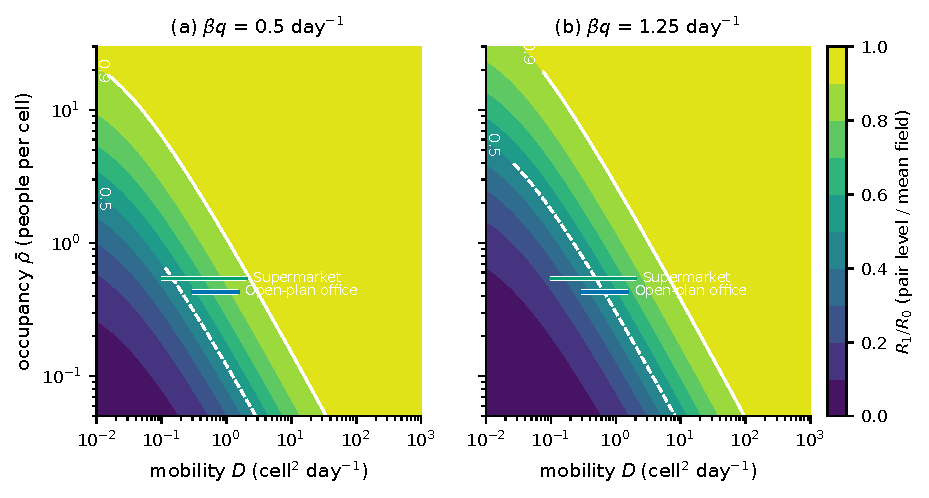
\includegraphics[width=\textwidth]{fig4_meanfield_validity_map_en}
\caption{Where the mean-field number is a good approximation of the pair-level number. Ratio
$\Rone/\Rz=1/\bigl(1+(\beta q/\rhobar)\gz\bigr)$ on the infinite homogeneous lattice
(Corollary~\ref{M-s5_pair:cor:infinite}; same-cell kernel, $\gamma=0.14\perday$) against the mobility $D$ and
the occupancy $\rhobar$ (other people per cell), for (a) $\beta q=0.5\perday$ and (b)
$\beta q=1.25\perday$. White contours: ratio $0.5$ (dashed) and $0.9$ (solid). Horizontal bars: occupancy
and range of zone mobilities at $\Dz=1$ of the office ($0.43$ people per cell, $D=0.3$--$1.5$) and
supermarket ($0.54$, $D=0.1$--$2.0$) scenes.}
\label{s5_pair:fig:validity}
% src: figure script code/bsc_sim/experiments/21_figures_more.py (fig_validity_map; closed form, no data
%      file); zone values code/bsc_sim/scenes/office.json, supermarket.json
\end{figure}

Figure~\ref{s5_pair:fig:validity} maps the ratio of the two levels on the infinite homogeneous lattice. At
$\rhobar=0.381$ and $\beta q=0.5\perday$ the ratio is $0.5$ at $D=0.24$,
$0.9$ at $D=3.5$ and $0.99$ at $D=52\cellday$; for $\beta q=1.25\perday$ these mobilities are $0.76$, $9.9$
and $143$. Higher occupancy moves the contours to lower mobility (ratio $0.9$ at $D=0.05$ for
$\rhobar=10$, $\beta q=0.5\perday$). The mean-field number is therefore adequate when many people share a
contact neighbourhood or when people move far enough during an infectious period to meet new ones. The
scenes at $\Dz=1$ satisfy neither condition. At $\Dz\approx2.4\times10^3\cellday$
(Section~\ref{M-s2_model:sec:regime}) the ratio on the infinite lattice is $0.9997$, and what remains in a
finite room is the well-mixed finite-population factor.
% src: data/s5_pair_checks.json (infinite: D_for_ratio_*; D=2400 ratio 0.99970)
%      mobility estimate: data/bsc_theory/worked_examples.json (E9_physical_D)

In the office at $\Dz=1$ the second generation of an index case and its direct cases is $1.63$ times the first
(Table~\ref{s5_pair:tab:mobility}). In unrestricted epidemics started from a uniformly placed index case the ratio is
lower still: the second generation is $1.29$ and $1.39$ times the first in the runs of the two simulators
(Section~\ref{M-s6_scenes:sec:outcomes}).
% src: data/bsc_sim/02_mobility.json (sim_gen2_over_gen1, R1_pair_ngm); data/s5_pair_checks.json
%      (mobility: gen_ratio_over_rhoK1; wellmixed_generation_ratio: 3.589 / 4.435 = 0.809;
%      saturation/office/full_epidemic_gen2_over_gen1: first implementation 1.293, second implementation 1.388);
%      data/bsc_sim/03_scenes.json (office|D0=1|range1m); code/bsc_sim/verify/v05_scenes.json (office|1.0|1m)

\subsection{A per-cell normalisation of the infection rate}\label{s5_pair:sec:percell}

\begin{remark}[Encounter factor; an approximation]\label{s5_pair:rem:encounter}
The pair hazard \eqref{M-s2_model:eq:pairhazard} is normalised by the mean number $\rhobar$ of \emph{other} people per
cell. A rule that infects each susceptible in a cell at rate $\beta q\,n_I/n_{\mathrm{tot}}$, with $n_I$ and
$n_{\mathrm{tot}}$ the instantaneous numbers of infectives and of all people in that cell, is a different process.
An infective who shares its cell with $k$ susceptible people then infects at total rate $\beta q\,k/(k+1)$, which is
zero when it is alone. If the other $\Npop-1$ people are taken to be independent of the infective and at
stationarity at every instant (an annealed approximation, appropriate when movement is fast), $k$ is binomial with
parameters $\Npop-1$ and $\pi_x$, and the identity $\binom{\Npop-1}{k}/(k+1)=\binom{\Npop}{k+1}/\Npop$ gives the
encounter factor
\[
  c_x=\Exp\Bigl[\frac{k}{k+1}\Bigr]=1-\frac{1-(1-\pi_x)^{\Npop}}{\Npop\,\pi_x},
\]
so that the exposure of a case under the per-cell rule is that of the mean-field model with $q_x$ replaced by
$c_xq_x$, and its reproduction number is approximately $\srad\bigl(\beta\Qm\diag(c)(\gamma\Id-\gen)^{-1}\bigr)$.
For 100 people on the 234 cells of the office $c=0.185$ (the index is alone in its cell with probability
$0.65$); for 100 people on $20\times20$ cells $c=0.114$. With a uniformly placed index case the annealed
estimates are $c\,\beta\langle q\rangle/\gamma=0.86$ and $0.41$. Exact simulation of the rule gives $0.690$
($0.676$--$0.704$) secondary cases in the office scene and $0.382$ ($0.372$--$0.392$) in the homogeneous
$20\times20$ room at $D=1$ ($20{,}000$ runs each; the second simulator gives $0.698\pm0.007$ and $0.384\pm0.005$),
and no run infected more than 37 and 23 people respectively: at these occupancies the per-cell rule is
sub-critical.

The annealed formula is not exact. In a homogeneous $20\times13$ room with 100 people and $q=1.4$ it predicts
$0.843$; simulation gives $0.825\pm0.013$ at $\Dz=10$ ($9{,}000$ runs), within about $5\,\%$, but
$0.754\pm0.022$ at $\Dz=1$ and $0.545\pm0.017$ at $\Dz=0.1$. In the two cases above it is too high by $7\,\%$
($20\times20$ room) and by $24\,\%$ (office, whose workstation cells have $D=0.3$). The reason is again the
repeated exposure of the same neighbours, which the annealed average ignores. In the four scenes at $\Dz=1$ the
per-cell rule gives $0.62$--$1.01$ secondary cases, a mean attack rate of $1.0$--$3.0\pct$, and at most $4.8\pct$ of
runs reach an attack rate of $10\pct$ (none of 2{,}000 in the metro carriage); it becomes supercritical only in the
crowded carriage at high mobility ($2.43$ secondary cases and a mean attack rate of $52\pct$ at $\Dz=100$).
\end{remark}
% src: data/bsc_theory/verify_theorems.json (encounter_factors: c 0.1848, 0.1142; 0.8427);
%      data/s5_pair_checks.json (encounter: prob_index_alone_in_cell 0.654, annealed_uniform_index 0.858,
%      annealed 0.408, counted_over_annealed 0.804 and 0.936, counted_check);
%      data/bsc_sim/01_validation.json (test E: 0.69025, 0.38195, max_final_size 37, 23);
%      code/bsc_sim/verify/ (per-cell rule, second simulator); code/bsc_theory/verify/v4_ibm_big.log (0.825 +- 0.013);
%      code/bsc_theory/verify/v3_dynamics.log (0.754 +- 0.022, 0.545 +- 0.017)
% src: data/bsc_sim/03_scenes.json: per-cell-rule columns: index offspring, attack_all, p_major (rows D0 = 1 and D0 = 100);
%      data/s6_scenes_numbers.json: summary_by_D0 (per-cell rule ranges)

% supp_sim.tex -- Supplementary Section S5: simulations of the scenes and of interventions; details.
% Paths in "% src:" comments are relative to the repository root.
% Table bodies between "% BEGIN AUTO" and "% END AUTO" are written by code/s6_scenes_tables.py; derived
% numbers: data/s6_scenes_numbers.json, data/s7_interventions_numbers.json and the files named.
\section{Simulations of the scenes and of interventions: details}\label{appS_sim:sec}

This section gives the details of Section~\ref{M-s6_scenes:sec} of the main text. Unless stated otherwise
$\beta=0.5\perday$, $\gamma=0.14\perday$, the contact kernel is the 1\,m kernel, there is one uniformly placed index
case, the room is occupied 24 hours a day, a `major' outbreak has an attack rate of at least 10\,\%, and $\Rhat$ is
the counted number of secondary cases of an index case that alone transmits. $\Ronebar$ and $\srad(\ngmone)$ are not
threshold quantities (Remark~\ref{M-s5_pair:rem:threshold}).

\subsection{The four scenes}\label{appS_sim:sec:scenes}

An epidemic in the office scene at $\Dz=1$ consists of about 5{,}900 events. Peak prevalence and peak day are the
maximum of $I/\Npop$ on a grid of $0.5$~day and its time, averaged over major outbreaks. The mean-field equations
are started from one infective spread uniformly over the cells, and from one infective placed in a single cell
(averaged over every third cell as seed); the extinction probabilities of \eqref{M-s6_scenes:eq:branching} are
computed by iteration from $s=0$. Fig.~\ref{s6_scenes:fig:curves} shows the epidemic curves of the four scenes
and Fig.~\ref{s6_scenes:fig:attack} the distribution of the attack rate over the same runs.
% src: data/bsc_sim/03_scenes.json: "office|D0=1|range1m".events_per_rep = 5919.5; code/bsc_sim/experiments/03_scenes.py (n_rep = 2000, T_MAX = 400 d); 03_scenes.json: n_unfinished = 0 in all 18 rows; code/s6_scenes_ode_pointseed.py

\begin{figure}[tbp]
\centering
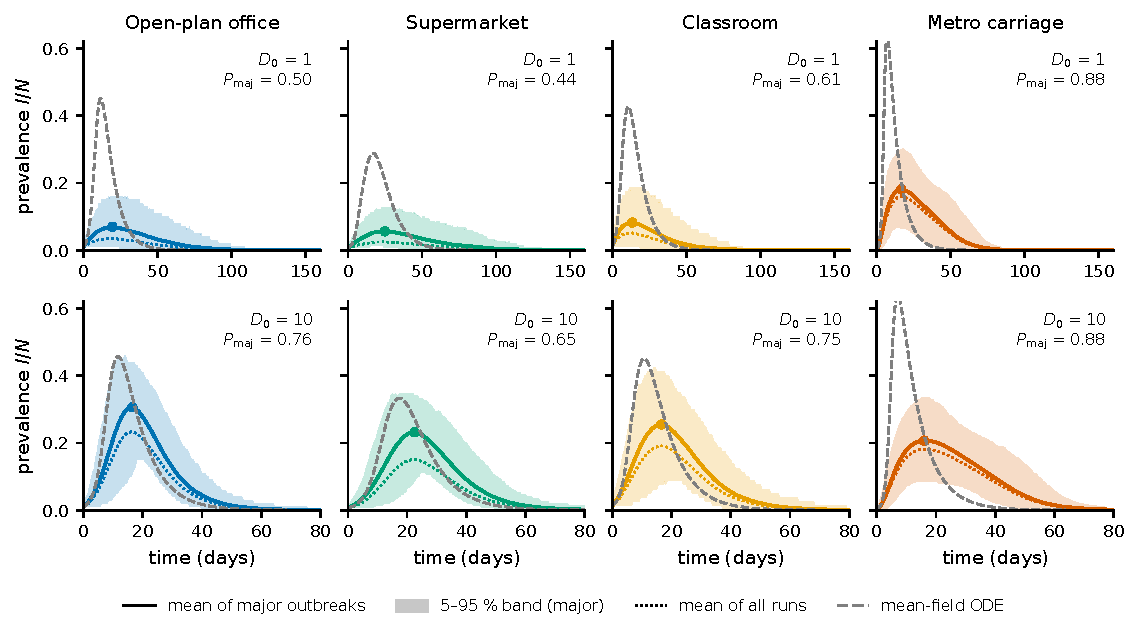
\includegraphics[width=\textwidth]{fig5_3_scene_epidemic_curves_en}
\caption{Prevalence $I/\Npop$ against time in the four scenes (columns; $\Npop=100$, $150$, $80$, $310$) at
$\Dz=1$ (top) and $\Dz=10\cellday$ (bottom); 1\,m kernel, 2{,}000 exact simulations per panel, one uniformly placed
index case. Solid line: mean over major outbreaks (attack rate at least $10\,\%$) at each time, with the band between
the 5th and 95th percentiles; the dot marks its maximum. Dotted: mean over all runs. Dashed: mean-field equations
\eqref{M-s2_model:eq:meanfield} started from one infective spread uniformly over the cells. The values of
$P_{\mathrm{maj}}$ in the panels are those of Table~\ref{M-s6_scenes:tab:scenes}. The maximum of the mean curve (office, $\Dz=1$: $7.0\,\%$
on day $19.5$) is lower than the mean of the individual peaks in Table~\ref{M-s6_scenes:tab:scenes} ($12.7\,\%$)
because outbreaks peak at different times.}
% src: figures/fig5_3_scene_epidemic_curves_en.pdf (code/bsc_sim/experiments/21_figures_more.py <- data/bsc_sim/03_curves_*.npz);
%      data/s6_scenes_numbers.json: scenes."office|D0=1".mean_curve_major_peak = 0.0696, _day = 19.5
\label{s6_scenes:fig:curves}
\end{figure}

\begin{figure}[tbp]
\centering
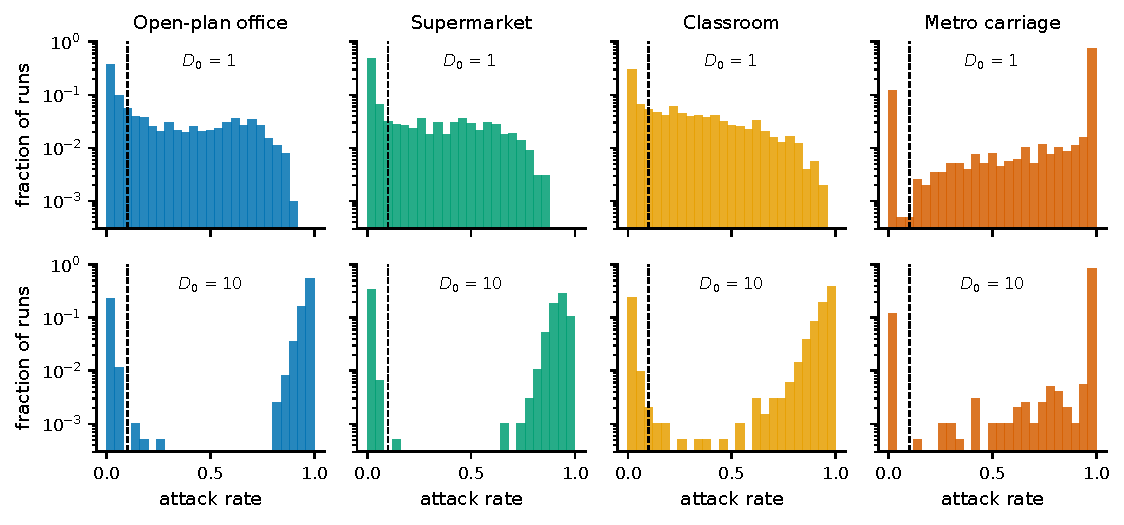
\includegraphics[width=\textwidth]{fig5_4_attack_rate_distributions_en}
\caption{Distribution of the attack rate (fraction of the $\Npop$ people ever infected) over the 2{,}000 runs of
each panel of Fig.~\ref{s6_scenes:fig:curves}; bins of width $0.04$, logarithmic vertical axis. The dashed line is
the $10\,\%$ threshold that defines a major outbreak. At $\Dz=10\cellday$ the distributions are bimodal; at $\Dz=1$
they are not, except in the metro carriage.}
% src: figures/fig5_4_attack_rate_distributions_en.pdf (code/bsc_sim/experiments/21_figures_more.py <- data/bsc_sim/03_curves_*.npz)
\label{s6_scenes:fig:attack}
\end{figure}

The values of $\Rhat$ in Table~\ref{M-s6_scenes:tab:scenes} come from separate batches of 2{,}000 runs and are the
least precise estimates of this quantity in the article; for the office, samples of 100{,}000 to 400{,}000
runs give $2.265\pm0.004$, $3.793\pm0.006$ and $4.340\pm0.015$ at $\Dz=1$, $10$ and $100$
(Section~\ref{M-s5_pair:sec:mobility}), in agreement with $\Ronebar$.
% src: data/s5_pair_large_sample.json (office|D0=1, office|D0=10, office|D0=100: mean, se, R1bar_exact)
The mean-field $\Rz$ does not: at $\Dz=1$ the index case of the office infects $2.26\pm0.06$ people where
$\Rz=5.11$, and the ratio $\Rhat/\Rz$ is $0.44$, $0.45$, $0.45$ and $0.60$ in the office, supermarket, classroom
and metro carriage. It rises to $0.84$--$0.93$ at $\Dz=100$.
% src: data/bsc_sim/03_scenes.json (R_index_alone_mean, R0_ngm); s6_scenes_numbers.json: scenes.*.Rhat_over_R0

With the same-cell kernel the mean field is not adequate for the outbreak probability where cells are smaller
than the contact range: in the metro carriage
$P_{\mathrm{br}}-P_{\mathrm{maj}}$ is $0.54$ at $\Dz=10$ ($0.888$ against $0.349$; attack rate of major
outbreaks $17.3\pct$ against $100.0\pct$) and still $0.031$ at $\Dz=100$ ($98.6\pct$ against $100.0\pct$); in the
classroom it is $0.08$ at $\Dz=10$ ($89.1\pct$ against $98.8\pct$) and $0.014$ at $\Dz=100$
(Section~\ref{s6_scenes:sec:kernel}).
% src: data/bsc_sim/03_scenes.json: "metro|D0=10|samecell" (p_major 0.349, p_major_branching 0.888, attack_major_mean 0.173, ode_attack 1.000),
%      "metro|D0=100|samecell" (0.858, 0.889, 0.986), "classroom|D0=10|samecell" (0.695, 0.777, 0.891, 0.988), "classroom|D0=100|samecell" (0.771, 0.785)

Peak height and peak day are a different matter. At $\Dz=10$ the simulated peaks ($39.0\,\%$, $30.6\,\%$, $35.0\,\%$,
$27.5\,\%$) are lower and about four to five days later than those of the mean-field equations even when these
are started from a single cell ($44.1\,\%$, $33.1\,\%$, $41.3\,\%$, $36.3\,\%$). At $\Dz=100$ the two agree to within $2.5$
percentage points and about one day in the office, the supermarket and the classroom. In the metro carriage they
do not: its mobility is $0.028\,\Dz$ on area average (Table~\ref{M-s2_model:tab:scenes}), the infection has to
travel along the 45 cells of the carriage, and the mean-field peak depends on the seed ($64.6\,\%$ on day $7.0$
for a uniform seed, $42.2\,\%$ on day $13.8$ for a single cell) and stays above the simulated $35.3\,\%$ on day
$16.5$.
% src: data/checks/simulation.json: metro_area_mean_D_over_D0 (0.0282, recomputed from scenes/metro.json; notes/VERIFICATION.md: Section 4.2, simulations, item 14)
% src: data/bsc_sim/03_scenes.json (peak_prev_major_mean, peak_time_major_mean, ode_peak_prev, ode_peak_time);
%      data/s6_scenes_ode_pointseed.json (point_seed.peak_mean, day_mean; rows D0 = 10 and 100)

\paragraph{Replication.}
The second simulator gave $P_{\mathrm{maj}}=0.498$, $0.429$, $0.603$ and $0.864$ for the four scenes at
$\Dz=1$ (3{,}000--4{,}000 runs each) and $0.734$ for the office at $\Dz=10$, against $0.496$, $0.436$, $0.614$,
$0.879$ and $0.762$ here. The two largest differences are $1.6$ and $2.1$ standard errors. The rows for
$\Dz=100$, the metro carriage at $\Dz=10$ and the same-cell rows at $\Dz\ge10$ were not re-run with the second simulator. Sampling prevalence every $0.5$ day lowers the reported peaks by $0.3$
to $1.0$ percentage point relative to the exact maximum.
% src: code/bsc_sim/verify/v05_scenes.json (p_major, n; peak_exact_major - peak_grid_major);
%      s6_scenes_numbers.json: check_scenes.*.z_first_minus_check (1.56, 2.11), peak_exact_minus_grid_points (0.28..0.96);
%      notes/VERIFICATION.md: Section 4.2, simulations, summary (D0 = 100 rows not re-simulated)

\subsection{Outbreak probability and early extinction}\label{s6_scenes:sec:pmajor}

\begin{table}[tbp]
\centering
\caption{Offspring distribution of a lone index case and the probability of a major outbreak (1\,m kernel;
$\Dz$ in \cdunit{}). Columns 3--6: mean, variance, variance-to-mean ratio and probability of zero of the
number of secondary cases when only the uniformly placed index case transmits (40{,}000 runs per row). Columns
7--9: probability that a branching process does not die out, for a Poisson offspring law with the simulated
mean, for the mean-field process \eqref{M-s6_scenes:eq:branching}, and for a Galton--Watson process with the
simulated offspring law. Last column: fraction of 2{,}000 full epidemics with attack rate at least $10\,\%$
(Table~\ref{M-s6_scenes:tab:scenes}).}
\label{s6_scenes:tab:pmajor}
% src: data/bsc_sim/03b_outbreak_probability.json (experiments/03b_outbreak_probability.py)
\footnotesize
\setlength{\tabcolsep}{4pt}
\begin{tabular}{@{}lrcccccccc@{}}
\toprule
 & & \multicolumn{4}{c}{secondary cases of a lone index} & \multicolumn{3}{c}{branching processes} & simulation\\
\cmidrule(lr){3-6}\cmidrule(lr){7-9}\cmidrule(l){10-10}
Scene & $\Dz$ & mean & variance & ratio & $P(0)$ & Poisson & mean field & Galton--Watson & $P_{\mathrm{maj}}$ (95\,\% CI)\\
\midrule
% BEGIN AUTO s6_scenes:tab:pmajor
Office & 1 & 2.27 & 6.0 & 2.66 & 0.269 & 0.857 & 0.781 & 0.613 & 0.496 (0.474--0.518)\\
Supermarket & 1 & 2.00 & 5.3 & 2.68 & 0.310 & 0.796 & 0.667 & 0.531 & 0.436 (0.414--0.458)\\
Classroom & 1 & 2.58 & 6.7 & 2.60 & 0.228 & 0.903 & 0.767 & 0.688 & 0.614 (0.592--0.635)\\
Metro & 1 & 5.54 & 21.0 & 3.80 & 0.109 & 0.996 & 0.888 & 0.877 & 0.879 (0.864--0.893)\\
\addlinespace
Office & 10 & 3.82 & 16.3 & 4.25 & 0.194 & 0.976 & 0.783 & 0.757 & 0.762 (0.743--0.781)\\
Supermarket & 10 & 2.89 & 11.0 & 3.80 & 0.253 & 0.932 & 0.685 & 0.658 & 0.648 (0.627--0.669)\\
Classroom & 10 & 3.73 & 15.5 & 4.15 & 0.197 & 0.973 & 0.777 & 0.753 & 0.750 (0.731--0.768)\\
Metro & 10 & 6.35 & 31.9 & 5.02 & 0.104 & 0.998 & 0.888 & 0.883 & 0.878 (0.863--0.892)\\
% END AUTO s6_scenes:tab:pmajor
\bottomrule
\end{tabular}
\end{table}

Early extinction of a chain started by one case occurs in every scene: the fraction of runs below the
$10\,\%$ threshold is $0.50$, $0.56$, $0.39$ and $0.12$ at $\Dz=1$ and $0.24$, $0.35$, $0.25$ and $0.12$ at
$\Dz=10$ (office, supermarket, classroom, metro carriage).
% src: data/bsc_sim/03_scenes.json: 1 - p_major (s6_scenes_numbers.json: scenes.*.die_out)
Table~\ref{s6_scenes:tab:pmajor} shows what determines it. The number of secondary cases of an index case is
over-dispersed, with a variance $2.6$ to $5.0$ times the mean, and $10\,\%$ to $31\,\%$ of index cases infect no one.
% src: 03b_outbreak_probability.json: var_over_mean (2.598..5.022), p_zero (0.104..0.310)
An exponential infectious period alone produces this much: a Poisson number of infections over an exponentially
distributed period is geometric, with a variance-to-mean ratio of one plus the mean ($3.0$ to $7.4$ here). The
simulated ratios are lower, consistent with the limited number of people within reach.
% src: s6_scenes_numbers.json: pmajor_ranges.geometric_var_over_mean_min/max (2.9975, 7.3503)
Over-dispersion lowers the outbreak probability \citep{lloydsmith2005superspreading}: a Poisson law with the same
mean would give $0.80$--$1.00$. A Galton--Watson process fed with the simulated offspring law reproduces
$P_{\mathrm{maj}}$ to within $0.011$ wherever the attack-rate distribution is bimodal (all scenes at $\Dz=10$, the
metro carriage at $\Dz=1$).
% src: s6_scenes_numbers.json: pmajor_ranges.gw_minus_sim_other_rows_max_abs = 0.0105; 03b: p_major_poisson_same_mean (0.796..0.998)

In the other three scenes at $\Dz=1$ the comparison depends on the convention, because the notion of a major
outbreak is not sharp there. With a threshold of $5\,\%$, $10\,\%$ or $20\,\%$ the office gives $0.60$, $0.50$ or
$0.40$, the supermarket $0.49$, $0.44$ or $0.37$ and the classroom $0.70$, $0.61$ or $0.49$, whereas at $\Dz=10$
the three thresholds change no value by more than $0.014$.
% src: s6_scenes_numbers.json: threshold_sensitivity_D0_10_max_change = 0.0135
% src: s6_scenes_numbers.json: scenes.*.P_attack_ge_5pct, P_attack_ge_10pct, P_attack_ge_20pct
%      (computed from data/bsc_sim/03_curves_*_range1m.npz: attack)
The Galton--Watson values ($0.61$, $0.53$, $0.69$) are $0.07$--$0.12$ above the $10\,\%$ fractions and within
$0.05$ of the $5\,\%$ fractions, so no conclusion about later generations can be drawn from them. The mean-field
branching values ($0.78$, $0.67$, $0.77$) are too high under either convention, by $0.15$--$0.29$ and
$0.07$--$0.19$.
% src: s6_scenes_numbers.json: pmajor.*.gw_minus_sim (0.117, 0.095, 0.074), pmajor.*.branching_minus_sim (0.285, 0.231, 0.153);
%      differences to the 5 % fractions: pmajor.*.gw_minus_sim_5pct (0.018, 0.045, -0.011), pmajor.*.branching_minus_sim_5pct (0.186, 0.180, 0.067)

\subsection{Sensitivity to the contact kernel}\label{s6_scenes:sec:kernel}

The contact kernel is a modelling choice with large consequences when cells are smaller than the contact range.
With the strict same-cell kernel the metro carriage ($0.5$\,m cells) produces no outbreak at
$\Dz=1$: none of 2{,}000 runs reaches an attack rate of $10\,\%$ (upper $95\,\%$ limit $0.002$; none of 3{,}000 in the
second simulator) and the mean attack rate is $1.1\,\%$, although $\Rz=9.84$.
% src: 03_scenes.json: "metro|D0=1|samecell" (n_major = 0, p_major_hi = 0.0019, attack_all_mean = 0.0112, R0_ngm = 9.836);
%      code/bsc_sim/verify/v05_scenes.json: "metro|1.0|same" (n = 3000, p_major = 0)
The index case does infect: $\Ronebar=1.51$, $\Rhat=1.56\pm0.04$, and the pair-level matrix has
$\srad(\ngmone)=2.24$. But passengers hardly move at this mobility, the people the index case can reach are those
who share its cell, and the cases it makes are born in that cell with no one left to infect: over the 2{,}000
full epidemics the second generation is $0.61$ times as numerous as the first.
% src: 03_scenes.json: "metro|D0=1|samecell" (R1_pair_uniform_index = 1.514, R_index_alone_mean = 1.562, _se = 0.038,
%      R1_pair_ngm = 2.244, gen2_over_gen1 = 0.608); re-check: v05_scenes.json "metro|1.0|same".gen2_over_gen1 = 0.609
With the 1\,m kernel the same carriage is the most explosive scene ($P_{\mathrm{maj}}=0.879$). In the classroom
the same-cell rule gives $P_{\mathrm{maj}}=0.276$ against $0.614$ with the 1\,m kernel, with
$\srad(\ngmone)=2.27$ and a generation ratio of $0.90$. The difference between the kernels fades with mobility
and is gone in the classroom at $\Dz=100$ ($0.771$ against $0.779$), not yet in the metro carriage ($0.858$
against $0.891$).
% src: 03_scenes.json: "classroom|D0=1|samecell" (p_major = 0.2755, R1_pair_ngm = 2.265, gen2_over_gen1 = 0.899),
%      "classroom|D0=100|samecell|range1m" (0.7715, 0.779), "metro|D0=100|samecell|range1m" (0.858, 0.891)
These cases are the evidence for Remark~\ref{M-s5_pair:rem:threshold}: $\Ronebar>1$ and $\srad(\ngmone)>1$ do not
imply that outbreaks occur, and neither does $\Rz>1$. Nothing computed in this article predicts the threshold
of the discrete system at low mobility; it has to be simulated.

\subsection{Where infections happen}

\begin{table}[tbp]
\centering
\caption{Where infections happen: prediction against simulation (1\,m kernel; $\Dz$ in \cdunit{}).
(a)~Pearson correlation $r$, over the walkable cells, between the predicted and the simulated distribution of
the cell in which the cases of generation $g=1,2,3$ are infected (40{,}000 outbreaks per row, uniformly placed
index case, generations 0--2 infectious); mean-field prediction $\propto\ngm^{g}\one$, pair-level prediction
$\propto\ngmone^{g}\one$. `Index alone': first generation in 100{,}000 runs in which only the index case
transmits, with the value of $r$ expected from sampling noise if the pair-level prediction is exact. Last column:
cases of generation~2 per outbreak, simulated / pair level / mean field. (b)~Office scene: share of the
infections of generation $g$ that occur in a class of cells divided by the share of the walkable floor it
occupies (1 = uniform).}
\label{s6_scenes:tab:hotspot}
% src (a): data/bsc_sim/04_spatial.json (r_meanfield, r_pair, mean_cases_per_run, pred_cases_per_run_*),
%          data/bsc_sim/04b_first_generation.json (r_meanfield, r_pair, r_expected_if_exact)
% src (b): data/s6_scenes_numbers.json: office_cell_classes (code/s6_scenes_tables.py, from
%          data/bsc_sim/04_spatial_office_D1.npz and 04_spatial_office_D10.npz)
\footnotesize
\setlength{\tabcolsep}{3pt}
\begin{tabular}{@{}lrcccccc@{}}
\multicolumn{8}{@{}l}{(a) Correlation between predicted and simulated infection maps}\\
\toprule
 & & \multicolumn{2}{c}{$r$, generations 1 / 2 / 3} & \multicolumn{3}{c}{$r$, index alone} & cases per outbreak,\\
\cmidrule(lr){3-4}\cmidrule(lr){5-7}
Scene & $\Dz$ & mean field & pair level & mean field & pair level & if exact & generation 2\\
\midrule
% BEGIN AUTO s6_scenes:tab:hotspot:a
Office & 1 & 0.09 / $-$0.23 / $-$0.37 & 0.88 / 0.82 / 0.71 & 0.284 & 0.948 & 0.958 & 2.8 / 5.2 / 21.8\\
Supermarket & 1 & 0.37 / 0.15 / 0.22 & 0.91 / 0.85 / 0.85 & 0.550 & 0.981 & 0.977 & 2.6 / 4.0 / 11.6\\
Classroom & 1 & 0.76 / 0.67 / 0.68 & 0.96 / 0.93 / 0.91 & 0.844 & 0.989 & 0.989 & 2.8 / 6.8 / 23.6\\
Metro & 1 & 0.76 / 0.69 / 0.57 & 0.92 / 0.95 / 0.91 & 0.876 & 0.980 & 0.979 & 8.1 / 31.6 / 82.8\\
\addlinespace
Office & 10 & 0.77 / 0.52 / 0.41 & 0.92 / 0.85 / 0.81 & 0.915 & 0.985 & 0.985 & 8.1 / 14.4 / 21.6\\
Supermarket & 10 & 0.97 / 0.97 / 0.98 & 0.99 / 0.99 / 0.99 & 0.981 & 0.996 & 0.996 & 6.3 / 8.3 / 10.9\\
Classroom & 10 & 0.96 / 0.96 / 0.96 & 0.98 / 0.98 / 0.97 & 0.984 & 0.996 & 0.996 & 6.8 / 14.1 / 22.7\\
Metro & 10 & 0.77 / 0.67 / 0.60 & 0.93 / 0.95 / 0.93 & 0.889 & 0.982 & 0.984 & 10.3 / 40.3 / 82.6\\
% END AUTO s6_scenes:tab:hotspot:a
\bottomrule
\end{tabular}

\vspace{1.5ex}
\begin{tabular}{@{}lrrrccc@{}}
\multicolumn{7}{@{}l}{(b) Office scene: relative infection rate by class of cells, generations 1 / 2 / 3}\\
\toprule
Class of cells & $\Dz$ & cells & floor (\%) & simulation & pair level & mean field\\
\midrule
% BEGIN AUTO s6_scenes:tab:hotspot:b
Workstations bordering a corridor & 1 & 56 & 23.9 & 1.13 / 1.24 / 1.35 & 1.13 / 1.16 / 1.18 & 1.08 / 1.02 / 0.98\\
Other workstations & 1 & 100 & 42.7 & 0.94 / 0.89 / 0.88 & 0.94 / 0.91 / 0.89 & 1.08 / 1.11 / 1.12\\
Corridor & 1 & 39 & 16.7 & 0.97 / 1.09 / 1.16 & 0.92 / 0.93 / 0.93 & 0.62 / 0.55 / 0.52\\
Meeting room & 1 & 26 & 11.1 & 1.00 / 0.88 / 0.68 & 1.06 / 1.12 / 1.16 & 1.15 / 1.29 / 1.44\\
Kitchen & 1 & 13 & 5.6 & 0.94 / 0.76 / 0.58 & 1.00 / 0.98 / 0.96 & 0.92 / 0.83 / 0.75\\
\addlinespace
Workstations bordering a corridor & 10 & 56 & 23.9 & 1.15 / 1.19 / 1.20 & 1.13 / 1.12 / 1.12 & 1.08 / 1.05 / 1.04\\
Other workstations & 10 & 100 & 42.7 & 1.06 / 1.08 / 1.09 & 1.06 / 1.07 / 1.07 & 1.08 / 1.08 / 1.08\\
Corridor & 10 & 39 & 16.7 & 0.71 / 0.72 / 0.72 & 0.68 / 0.67 / 0.67 & 0.62 / 0.60 / 0.59\\
Meeting room & 10 & 26 & 11.1 & 0.93 / 0.81 / 0.76 & 1.04 / 1.05 / 1.05 & 1.15 / 1.24 / 1.30\\
Kitchen & 10 & 13 & 5.6 & 0.87 / 0.79 / 0.78 & 0.89 / 0.84 / 0.81 & 0.92 / 0.87 / 0.84\\
% END AUTO s6_scenes:tab:hotspot:b
\bottomrule
\end{tabular}
\end{table}

\begin{figure}[tbp]
\centering
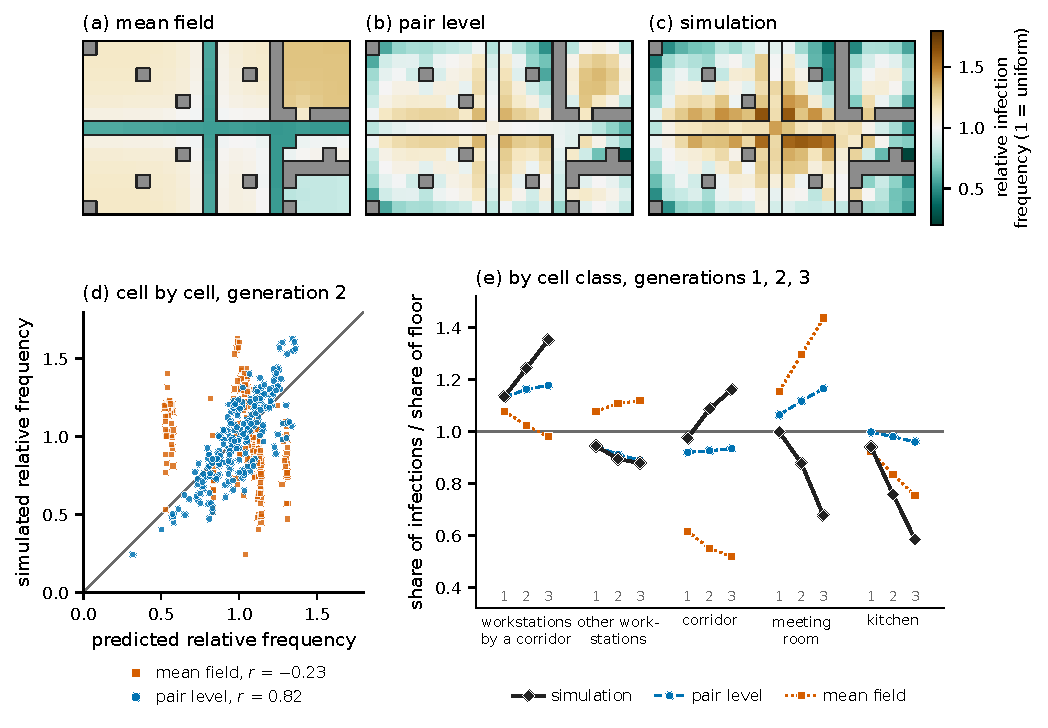
\includegraphics[width=\textwidth]{fig5_2_spatial_pattern_en}
\caption{Where infections happen in the office scene at $\Dz=1\cellday$ ($\Npop=100$, 234 walkable cells, 1\,m
kernel, equal to the same-cell kernel here; 40{,}000 outbreaks from a uniformly placed index case, generations 0--2
infectious). (a)--(c)~Frequency with which the cases of generation~2 are infected in each cell, relative to a
uniform distribution: mean-field prediction $\propto\ngm^2\one$, pair-level prediction $\propto\ngmone^2\one$,
and simulation. Grey cells are barriers; thin lines separate the zones of Fig.~\ref{M-s2_model:fig:scenes} (the
cross is the corridor, the block at the top right the meeting room, the block at the bottom right the kitchen).
(d)~The same three maps cell by cell, with the correlation coefficients $r$ of
Table~\ref{s6_scenes:tab:hotspot}. (e)~Share of infections divided by share of floor for five classes of cells
and generations 1, 2, 3 (numbers in Table~\ref{s6_scenes:tab:hotspot}b).}
% src: code/s6_scenes_fig_spatial.py <- data/bsc_sim/04_spatial_office_D1.npz, 04_spatial.json,
%      data/s6_scenes_numbers.json (office_cell_classes); output figures/fig5_2_spatial_pattern_{en,zh}.pdf
\label{s6_scenes:fig:spatial}
\end{figure}

For a uniformly placed index case the cell in which a case of generation $g$ is infected has a distribution
proportional to $\ngm^{g}\one$ in the mean-field model and, in the pair-level description, to $\ngmone^{g}\one$.
Table~\ref{s6_scenes:tab:hotspot}(a) compares both with the infection trees of 40{,}000 outbreaks per scene.

In the office at $\Dz=1$ the mean-field map is uncorrelated with the simulated one in the first generation and
anti-correlated in the next two ($r=0.09$, $-0.23$, $-0.37$), whereas the pair-level map gives $r=0.88$, $0.82$,
$0.71$. The second simulator gives $0.11$, $-0.23$, $-0.37$ and $0.88$, $0.82$, $0.73$.
% src: data/bsc_sim/04_spatial.json: "office|D0=1".gen1..3 (r_meanfield 0.092, -0.235, -0.371; r_pair 0.875, 0.816, 0.709);
%      code/bsc_sim/verify/v07_hotspot.json: gen1..3 (r_mf 0.105, -0.234, -0.366; r_pair 0.878, 0.824, 0.726)
The pair-level map is exact for the first generation of a lone index case, and the simulation is compatible with
that: with only the index case transmitting, $r=0.948$ where $0.958$ is expected from sampling noise, and the
goodness-of-fit statistic is between $0.85$ and $1.20$ per degree of freedom in the eight rows (smallest
$p$-value $0.02$, office at $\Dz=1$).
% src: data/bsc_sim/04b_first_generation.json (r_pair, r_expected_if_exact, chi2_pair, dof);
%      s6_scenes_numbers.json: first_generation_chi2 (chi2_over_dof_min = 0.846, _max = 1.203; p = 0.0186)
For later generations it is an approximation, and it over-predicts their size, because a new case starts inside
the cluster of its infector: in generation~2 there are $2.8$ cases per outbreak in the simulation, $5.2$ in the
pair-level description and $21.8$ in the mean field.
% src: 04_spatial.json: "office|D0=1".gen2 (mean_cases_per_run = 2.769, pred_cases_per_run_pair = 5.167, pred_cases_per_run_mf = 21.76)
Over all scenes at $\Dz=1$ the pair-level correlation lies between $0.71$ and $0.96$ and the mean-field one between $-0.37$ and $0.76$.
At $\Dz=10$ the mean-field map is adequate in the supermarket and the classroom ($r=0.96$--$0.98$) but not in
the office ($0.77$, $0.52$, $0.41$) or the metro carriage ($0.77$, $0.67$, $0.60$).
% src: s6_scenes_numbers.json: hotspot_pair_r_range_D0_1 (0.709, 0.957), hotspot_meanfield_r_range_D0_1 (-0.371, 0.764);
%      04_spatial.json rows D0 = 10

Which cells are hot is shown in Fig.~\ref{s6_scenes:fig:spatial} and Table~\ref{s6_scenes:tab:hotspot}(b). The
mean-field map of the first generation is proportional to $q$: it marks the meeting room ($q=1.5$) and the
workstations ($q=1.4$) and leaves the corridor ($q=0.8$) cold, at $0.62$ of the uniform rate. In the simulation
at $\Dz=1$ the corridor is close to average. With only the index case transmitting it receives $15.4\,\%$ of the
infections on $16.7\,\%$ of the floor (pair level $15.3\,\%$, mean field $10.3\,\%$), and in full outbreaks its
relative rate is $0.97$, $1.09$ and $1.16$ in generations 1--3.
% src: code/bsc_sim/verify/v07_hotspot.json: zone_C (obs 0.1537, pair 0.1532, mf 0.1026, area 0.1667; 100 000 runs);
%      s6_scenes_numbers.json: office_cell_classes."D0=1".classes.C.sim (0.974, 1.087, 1.160), .meanfield[0] = 0.615
So the corridors are not the hotspots. The hottest cells are workstation cells that border a corridor: their
relative rate is $1.13$, $1.24$ and $1.35$, against $0.94$, $0.89$ and $0.88$ for the other workstation cells
(second simulator: $1.15$, $1.26$, $1.36$ and $0.94$, $0.88$, $0.87$), and in each generation at least 14 of
the 15 hottest cells are workstation cells, 13 to 15 of them next to a corridor.
% src: s6_scenes_numbers.json: office_cell_classes."D0=1".classes.W_border.sim, .W_interior.sim, .top15 (zones, n_border_workstations);
%      data/checks/simulation.json: office_hotspots_D0_1.relative_rate_generations_1_3 (values of the re-check;
%      notes/VERIFICATION.md: Section 4.2, simulations, item 6)
A plausible reason is that these cells combine a high $q$ with a faster exchange of neighbours: the hop rate
\eqref{M-s2_model:eq:hop} across a workstation--corridor edge is $0.5\,\Dz$ against $0.3\,\Dz$ between two
workstation cells. The meeting room, the hotspot of the mean-field analysis of Section~\ref{M-s4_geometry:sec},
falls from the average rate to $0.68$ by the third generation, where the mean field predicts $1.44$. This is
consistent with local depletion: only about 11 of the 100 people are in it at any time and, at this mobility,
few others arrive.
% src: office_cell_classes."D0=1".classes.M.sim (0.998, 0.877, 0.677), .meanfield (1.154, 1.295, 1.436);
%      hop rates: 2*0.3*1.5/(0.3+1.5) = 0.5 and 0.3 (code/bsc_sim/scenes/office.json: D_W = 0.3, D_C = 1.5); 26/234 x 100 = 11.1
At $\Dz=10$ the corridor is cold in the simulation as well ($0.71$--$0.72$; mean field $0.59$--$0.62$) and the
workstation cells are above average whether or not they border a corridor ($1.15$--$1.20$ and $1.06$--$1.09$).
% src: office_cell_classes."D0=10".classes (C.sim, C.meanfield, W_border.sim, W_interior.sim)
A statement such as `infection concentrates in the meeting room and at the workstations' is thus a mean-field
statement. For discrete people at low mobility the map has to be taken from $\ngmone$ or from simulation, and
all of this concerns a room whose occupants perform a random walk without home positions.

\subsection{Ranking of the scenes}\label{s6_scenes:sec:ranking}

At $\Dz=1$ the four scenes rank in the same order, metro carriage, classroom, office, supermarket, by $\Rz$
($9.24$, $5.87$, $5.11$, $4.39$), by $\Rhat$ ($5.59$, $2.62$, $2.26$, $1.97$), by $P_{\mathrm{maj}}$ and by the
attack rate over all runs.
% src: 03_scenes.json (R0_ngm, R_index_alone_mean, p_major, attack_all_mean at D0 = 1); s6_scenes_numbers.json: ranking_D0_1
The order is not robust. The attack rate of major outbreaks at $\Dz=1$ is lowest in the classroom ($39.2\,\%$),
and at $\Dz=10$ the office and the classroom cannot be told apart ($\Rhat=3.90\pm0.09$ and $3.72\pm0.09$;
$P_{\mathrm{maj}}=0.762$ and $0.750$).
% src: 03_scenes.json rows D0 = 10; s6_scenes_numbers.json: ranking_D0_1.by_attack_major, ranking_D0_10
Above all, the ranking belongs to the closed-room idealisation, in which the same people share the room for the
whole infectious period of $1/\gamma=7.1$ days. Nobody spends a week in a metro carriage. Counted per visit at
$\Dz=1$, an index case causes $0.175$ infections in an office day of 8 hours, $0.027$ in a one-hour lecture,
$0.018$ in a 20-minute metro ride and $0.008$ in a supermarket visit of 27 minutes
(Section~\ref{M-s6_scenes:sec:interventions}, Table~\ref{M-s7_interventions:tab:dwell}), which puts the office first and the
metro carriage third.
% src: data/bsc_sim/11_dwell_time.json: per_visit_sim (office 0.1753, classroom 0.0270, metro 0.0178, supermarket 0.0083),
%      visit_hours (8, 1, 0.333, 0.45)

\subsection{Heterogeneity of the infection efficiency}\label{s7_interventions:sec:hetero}

\begin{figure}[tbp]
  \centering
  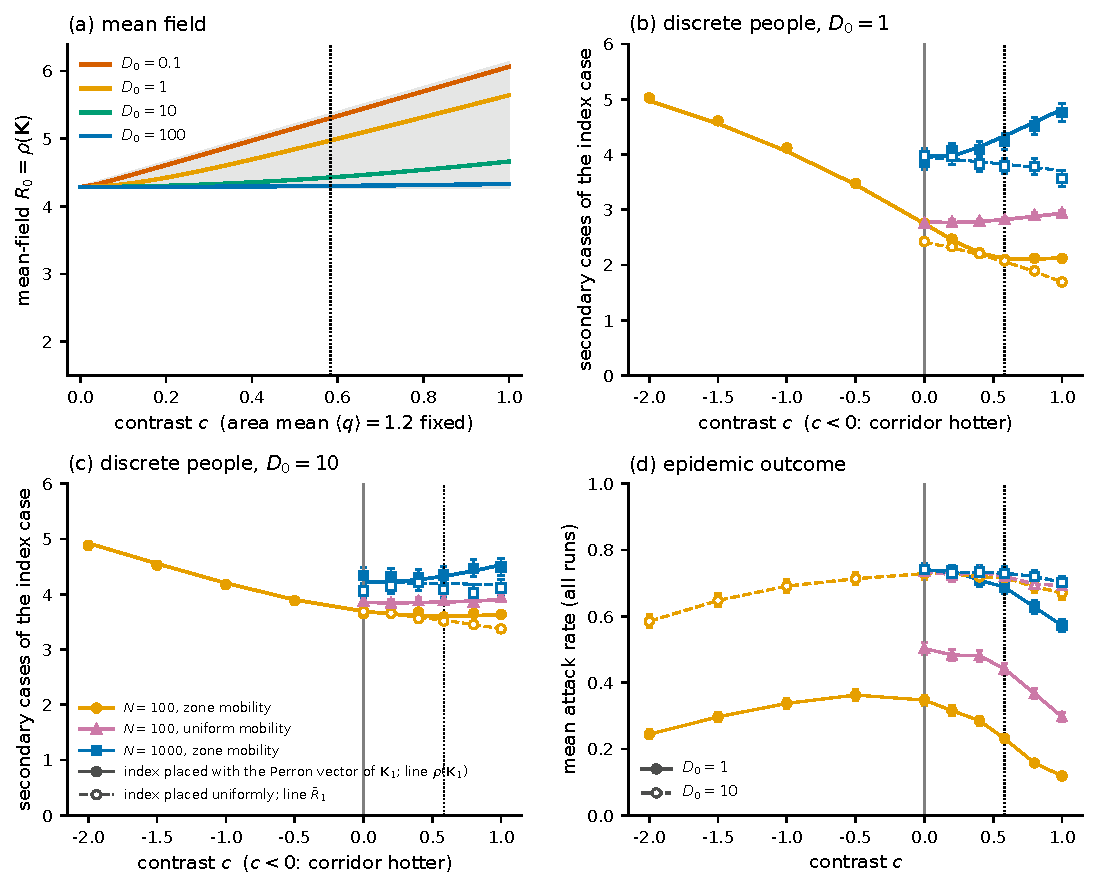
\includegraphics[width=\textwidth]{s7_interventions_hetero_en}
  \caption{Two-zone room ($20\times13$ cells; workspace 70\,\% of the floor with mobility $0.3\Dz$, corridor
  30\,\% with $2\Dz$; same-cell kernel; FD) as a function of the contrast $c$ of
  \eqref{M-s7_interventions:eq:contrast}; the dotted vertical line marks $c=0.583$ ($q_{\mathrm W}=1.5$,
  $q_{\mathrm C}=0.5$). (a)~Mean-field $\Rz$ for four mobility scales; the grey band is the interval
  $[\beta\langle q\rangle/\gamma,\beta\qmax/\gamma]$ of Theorem~\ref{M-s3_r0:thm:bounds}.
  (b,\,c)~Counted secondary cases $\Rhat$ of the index case (only the index transmits; 95\,\% intervals;
  20,000 runs per point for $\Npop=100$, 4,000 for $\Npop=1000$) at $\Dz=1$ and $\Dz=10$. Filled symbols: index
  placed with the Perron vector of the pair-level matrix $\ngmone$, to be compared with $\srad(\ngmone)$ (solid
  lines). Open symbols: index placed uniformly, to be compared with $\Ronebar$ (dashed lines). `Uniform
  mobility' is the control with $D=0.81\Dz$ in every cell (Perron-placed index only).
  (d)~Mean attack rate over all runs with 95\pct{} intervals (2,000 epidemics per point), $\Dz=1$
  (filled, solid) and $\Dz=10$ (open, dashed). Numbers in Table~\ref{s7_interventions:tab:hetero}.}
  % src: code/s7_interventions_fig_hetero.py <- data/bsc_sim/05_heterogeneity.json, 05_heterogeneity_extra.json, data/s7_interventions_hetero_se.json (panel d)
  \label{s7_interventions:fig:hetero}
\end{figure}

The two-zone room of Fig.~\ref{s7_interventions:fig:hetero} has $20\times13$ cells without barriers, a lattice
spacing of 1.5\,m (so that the 1\,m kernel is the same-cell kernel), FD calibration, and $\Npop=100$ (0.38 other
people per cell) or $\Npop=1000$ (3.8). The contrast $c$ of \eqref{M-s7_interventions:eq:contrast} is $0$ in the
uniform room, $0.583$ for $q_{\mathrm W}=1.5$, $q_{\mathrm C}=0.5$, and negative when the higher efficiency is in
the corridor. Table~\ref{s7_interventions:tab:hetero} gives the numbers. The mean-field $\Rz$ is $4.972$ at
$c=0.583$ and $\Dz=1$, and $4.427$ ($+3.3\,\%$) at $\Dz=10$.
% src: code/bsc_sim/experiments/05_heterogeneity.py (set-up); data/bsc_sim/05_heterogeneity.json keys D0=1|N=100|c=0.5833, D0=10|N=100|c=0.5833 (R0_ngm)

\begin{table}[tbp]
  \centering\footnotesize\setlength{\tabcolsep}{3.5pt}
  \caption{Two-zone room of Fig.~\ref{s7_interventions:fig:hetero} (same-cell kernel, FD): mean-field $\Rz$,
  pair-level $\srad(\ngmone)$, counted secondary cases $\Rhat$ (95\pct{} interval; 20,000 runs for $\Npop=100$,
  4,000 for $\Npop=1000$) for an index placed with the Perron vector of $\ngmone$ and for a uniformly placed
  index, probability of a major outbreak and mean attack rate over all runs ($\pm$ standard error; 2,000
  epidemics per row). Mobility `zones': $0.3\Dz$ in the workspace and $2\Dz$ in the corridor; `uniform':
  $0.81\Dz$ everywhere; $c=-2$ is the hot-corridor control. $^{\dagger}$From the
  verification (20,000 runs; standard error 0.02 to 0.03); not simulated in the main runs.}
  \label{s7_interventions:tab:hetero}
  % src: data/s7_interventions_tables.tex (generated by code/s7_interventions_numbers.py) <- data/bsc_sim/05_heterogeneity.json, 05_heterogeneity_extra.json; dagger entries: code/bsc_sim/verify/v09_het.json (sim_uniform); last two columns: data/s7_interventions_hetero_se.json (stored|... for N = 100: the stored 2,000-run batches re-run from their seeds; new|... for N = 1000: 2,000 further epidemics, seed 5503, in place of the 300 stored ones)
  \begin{tabular}{@{}rrlccccccc@{}}
    \toprule
    $\Dz$ & $\Npop$ & mobility & $c$ & $\Rz$ & $\srad(\ngmone)$ & $\Rhat$, Perron index & $\Rhat$, uniform index & $P(\text{major})$ & attack \\
    \midrule
    1 & 100 & zones & 0.00 & 4.29 & 2.75 & 2.75 (2.71--2.79) & 2.42 (2.39--2.46) & $0.541\pm0.011$ & $0.347\pm0.008$ \\
     &  &  & 0.58 & 4.97 & 2.12 & 2.10 (2.07--2.13) & 2.07 (2.04--2.11) & $0.460\pm0.011$ & $0.231\pm0.006$ \\
     &  &  & 1.00 & 5.64 & 2.13 & 2.12 (2.09--2.15) & 1.69 (1.66--1.72) & $0.345\pm0.011$ & $0.119\pm0.004$ \\
    1 & 1000 & zones & 0.00 & 4.29 & 3.97 & 3.87 (3.74--3.99) & 3.97 (3.84--4.11) & $0.766\pm0.009$ & $0.740\pm0.009$ \\
     &  &  & 0.58 & 4.97 & 4.33 & 4.23 (4.09--4.37) & 3.79 (3.65--3.93) & $0.727\pm0.010$ & $0.688\pm0.009$ \\
     &  &  & 1.00 & 5.64 & 4.82 & 4.76 (4.60--4.92) & 3.57 (3.42--3.71) & $0.639\pm0.011$ & $0.573\pm0.010$ \\
    1 & 100 & uniform & 0.00 & 4.29 & 2.78 & 2.76 (2.72--2.80) & 2.76$^{\dagger}$ & $0.646\pm0.011$ & $0.503\pm0.009$ \\
     &  &  & 0.58 & 4.76 & 2.82 & 2.82 (2.78--2.86) & 2.61$^{\dagger}$ & $0.620\pm0.011$ & $0.442\pm0.008$ \\
    1 & 100 & zones & $-2.00$ & 9.14 & 4.97 & 5.02 (4.96--5.09) & 2.50$^{\dagger}$ & $0.381\pm0.011$ & $0.244\pm0.007$ \\
    \midrule
    10 & 100 & zones & 0.00 & 4.29 & 3.69 & 3.65 (3.59--3.70) & 3.69 (3.64--3.75) & $0.748\pm0.010$ & $0.729\pm0.009$ \\
     &  &  & 0.58 & 4.43 & 3.60 & 3.59 (3.54--3.64) & 3.52 (3.46--3.57) & $0.744\pm0.010$ & $0.717\pm0.009$ \\
     &  &  & 1.00 & 4.66 & 3.63 & 3.64 (3.58--3.69) & 3.37 (3.32--3.43) & $0.704\pm0.010$ & $0.671\pm0.010$ \\
    10 & 1000 & zones & 0.00 & 4.29 & 4.22 & 4.34 (4.19--4.49) & 4.06 (3.92--4.20) & $0.753\pm0.010$ & $0.742\pm0.009$ \\
     &  &  & 0.58 & 4.43 & 4.33 & 4.35 (4.21--4.50) & 4.08 (3.94--4.23) & $0.745\pm0.010$ & $0.730\pm0.010$ \\
    10 & 100 & uniform & 0.58 & 4.36 & 3.86 & 3.89 (3.84--3.95) & -- & $0.737\pm0.010$ & $0.720\pm0.009$ \\
    10 & 100 & zones & $-2.00$ & 5.70 & 4.93 & 4.89 (4.82--4.96) & -- & $0.614\pm0.011$ & $0.585\pm0.010$ \\
    \bottomrule
  \end{tabular}
\end{table}

\paragraph{Discrete individuals, $\Dz=1$, $\Npop=100$.} Everything that is counted \emph{falls} when the contrast
is switched on (Fig.~\ref{s7_interventions:fig:hetero}b,d; numbers in Table~\ref{s7_interventions:tab:hetero}): $\Rhat$ of
an index case placed with the Perron vector of $\ngmone$ goes from $2.75$ to $2.10$ ($-24\,\%$), $\Rhat$ of a
uniformly placed index from $2.42$ to $2.07$ ($-15\,\%$), the ratio of second- to first-generation cases
from $2.19$ to $1.58$ ($-28\,\%$), the probability of a major outbreak from $0.541$ to $0.460$ and the mean
attack rate from $0.347$ to $0.231$ ($-33\,\%$).
% src: data/bsc_sim/05_heterogeneity.json keys D0=1|N=100|c=0.0000 and c=0.5833 (sim_R_perron, sim_R_uniform, sim_gen2_over_gen1, p_major, attack_all); data/s7_interventions_numbers.json hetero/changes_D1_N100
(The second simulator gives $2.77\pm0.02\to2.11\pm0.02$ and $0.341\to0.239$ for the first
and the last of these.)
% src: code/bsc_sim/verify/v09_het.json keys <zone variant>|D0=1.0|N=100|c=0.000, c=0.583
The cause is not the heterogeneity of $q$ as such but its coincidence with low mobility: this layout puts
the high efficiency where people hardly move, where an infective keeps meeting the same neighbours and its
contacts fall on people who are already infected (Section~\ref{M-s5_pair:sec}). Two controls confirm this. With
the same contrast and \emph{uniform} mobility ($0.81\,\Dz$ everywhere, the area mean) $\Rhat$ rises slightly,
$2.76\to2.82$; with the high efficiency in the \emph{mobile} corridor ($c=-2$) $\Rhat$ of a Perron-placed
index reaches $5.02$.
% src: data/bsc_sim/05_heterogeneity_extra.json keys extra|uniformD|D0=1|N=100|c=0.0000, c=0.5833; extra|<zone variant>|D0=1|N=100|c=-2.0000 (sim_R_perron)
In both controls the mean attack rate nevertheless falls ($0.503\to0.442$ and $0.347\to0.244$): a low-$q$
zone is a place where an index case tends to fizzle and which the epidemic reaches late.
% src: data/bsc_sim/05_heterogeneity_extra.json (attack_all), same keys

\paragraph{High occupancy.} With $\Npop=1000$ the pair-level $\srad(\ngmone)$ rises with the contrast
($3.97$, $4.33$, $4.82$ at $c=0$, $0.58$, $1$), and so does $\Rhat$ of a Perron-placed index ($3.87$, $4.23$,
$4.76$; re-check $3.92$, $4.33$, $4.78$, each $\pm0.08$ to $0.09$).
% src: data/bsc_sim/05_heterogeneity.json keys D0=1|N=1000|c=... (R1_pair_ngm, sim_R_perron); code/bsc_sim/verify/v09_het.json keys <zone variant>|D0=1.0|N=1000|c=... (sim_perron, se)
This is the only sense in which the simulation shows the rise of $\Rz$. For a uniformly placed index the
count falls in these runs ($3.97$, $3.79$, $3.57$; re-check $3.96$, $3.86$, $3.82$). It is bounded above by
$\beta\langle q\rangle/\gamma=4.29$ for every contrast (Proposition~\ref{M-s5_pair:prop:saturation}), so it
cannot follow the rise of $\Rz$; but it is not monotone in the contrast in general: with the high efficiency
in the mobile corridor ($c<0$, $\Npop=100$) $\Ronebar$ rises from $2.41$ at $c=0$ to $2.66$ at $c=-1$ before
falling to $2.44$ at $c=-2$ ($\Dz=1$), and from $3.69$ to $3.81$ at $\Dz=10$.
% src: data/bsc_sim/05_heterogeneity.json keys D0=1|N=1000|c=... (sim_R_uniform; 4000 counted runs); code/bsc_sim/verify/v09_het.json (sim_uniform)
% src: data/bsc_sim/05_heterogeneity.json D0=1|N=100|c=0.0000 (R1_pair_uniform 2.411), D0=10 (3.688); data/bsc_sim/05_heterogeneity_extra.json extra|<zone variant>|D0=1|N=100|c=-0.5 ... -2.0 (R1_pair_uniform 2.589, 2.662, 2.623, 2.441), D0=10|c=-1.0 (3.808)
The outbreak probability and the mean attack rate fall as well: in 2{,}000 epidemics per contrast they are
$0.766\pm0.009$, $0.727\pm0.010$, $0.639\pm0.011$ and $0.740\pm0.009$, $0.688\pm0.009$, $0.573\pm0.010$
(standard errors). The first sample of 300 epidemics per contrast ($0.737$, $0.690$, $0.630$ and $0.712$,
$0.654$, $0.564$, each $\pm0.025$ to $0.028$) resolved only the difference between $c=0$ and $c=1$. $\Rz$ is
the growth factor per generation once cases are distributed as the incidence map $\wvec$, not the fate of a
typical introduction.
% src: data/s7_interventions_hetero_se.json keys new|D0=1|N=1000|c=0.0000, 0.5833, 1.0000 (p_major, p_major_se, attack_all, attack_all_se; n = 2000, seed 5503); stored|D0=1|N=1000|c=... (n = 300; p_major_se 0.025-0.028, attack_all_se 0.025; reproduces_stored true); code/s7_interventions_hetero_se.py

\paragraph{$\Dz=10$.} For $\Npop=100$ the contrast $c=0.583$ changes $\Rhat$ of a Perron-placed index from $3.65$ to
$3.59$, the outbreak probability from $0.748$ to $0.744$ and the mean attack rate from $0.729$ to $0.717$
(all less than 2\pct, and within one standard error of $0.010$ for the last two); $\Rhat$ of a uniformly
placed index falls by 5\pct{} ($3.69\to3.52$) (Fig.~\ref{s7_interventions:fig:hetero}c,d). For $\Npop=1000$
the outbreak probability is $0.753\pm0.010$ and $0.745\pm0.010$ at $c=0$ and $0.58$, and the mean attack rate
$0.742\pm0.009$ and $0.730\pm0.010$: no change is resolved.
% src: data/bsc_sim/05_heterogeneity.json keys D0=10|N=100|c=0.0000, c=0.5833; data/s7_interventions_numbers.json hetero/changes_D10_N100; data/s7_interventions_hetero_se.json keys stored|D0=10|N=100|c=... (p_major_se, attack_all_se), new|D0=10|N=1000|c=0.0000, 0.5833

\subsection{Barriers with identical starts}\label{s7_interventions:sec:barriers}

To isolate the effect of barriers we use a uniform room ($20\times13$ cells, $\Npop=100$, $q=1.2$, so
$\beta q/\gamma=4.29$, uniform mobility $D$, same-cell kernel) and close randomly chosen cells at a nominal
density $\rho_B$. The barrier sets of one layout are nested; walkable pockets cut off by barriers are closed
as well, so that the realised density at nominal $0.30$ is $0.35$. In all arms of a layout the same people
start on the same cells (drawn from the cells that are walkable in the densest arm), the index case is the
same person on the centre cell, and each replicate uses the same random seed: the arms differ only by the
barriers. Fig.~\ref{s7_interventions:fig:barriers} shows a scan over seven
densities at $D=1$; Table~\ref{s7_interventions:tab:barriers} gives the
effects for 40 further layouts at $D=1$ and $D=10$, with standard errors across layouts, and for the
re-check's 40 layouts.
% src: code/bsc_sim/experiments/06_obstacles.py (design); code/s7_interventions_barriers.py; code/bsc_sim/verify/v08b_obstacles_many.py; realised density: data/s7_interventions_barriers.json D=1/arms/rhoB=0.30|FD/realised = 0.352

\begin{enumerate}[label=(\roman*),leftmargin=*,itemsep=2pt,topsep=3pt]
\item \emph{Mean field.} Under FD, $\Rz=\beta q/\gamma=4.29$ at every barrier density
  (Theorem~\ref{M-s4_geometry:thm:closed}). Under DD it rises as the floor shrinks,
  by \eqref{M-s7_interventions:eq:dd}: $4.76$ at 10\,\% and $6.7$ at nominal 30\,\%.
  % src: data/s7_interventions_barriers.json D=1/arms/rhoB=0.10|DD, rhoB=0.30|DD (R0); data/bsc_sim/06_obstacles.json (R0_ngm)
\item \emph{Pair level.} Under FD the pair-level $\Rone$ of the centre index falls a little, $3.02\to2.94\to2.80$
  at $\rho_B=0$, $0.10$, $0.30$ for $D=1$ and $3.90\to3.87\to3.75$ for $D=10$: barriers lengthen the time two
  people remain neighbours.
\item \emph{Outcomes at $D=1$, FD.} The mean attack rate falls by $0.040\pm0.003$ at 10\,\% barriers and by
  $0.223\pm0.011$ at 30\,\% (re-check: $0.047\pm0.004$ and $0.235\pm0.011$), the peak prevalence of major
  outbreaks from 27\pct{} to 25\pct{} and 18\pct, while the outbreak probability falls much
  less ($0.70\to0.69\to0.62$). Barriers act by stopping outbreaks part-way on a fragmented floor, not by
  preventing take-off.
\item \emph{Peak time at $D=1$, FD.} The peak of major outbreaks is delayed by $0.81\pm0.12$ day at 10\,\%
  barriers (re-check: $0.82\pm0.10$) and by $0.93\pm0.23$ day at 30\,\% (re-check: $0.71\pm0.30$): a real delay
  of about 0.8 day. The scan of
  Fig.~\ref{s7_interventions:fig:barriers}c cannot resolve it (its across-layout intervals are $\pm1.1$ day or
  wider).
\item \emph{$D=10$, FD.} Barriers at 10\,\% leave the attack rate unchanged ($+0.005\pm0.005$) and at 30\,\%
  lower it by $0.025\pm0.005$; the peak is lower by 0.8 and 5.3 percentage points and later by $0.34\pm0.05$
  and $2.05\pm0.16$ days.
\item \emph{DD.} Barriers also crowd people together. At $D=1$ the two effects cancel at 10\,\%
  ($-0.001\pm0.004$) and fragmentation wins at 30\,\% ($-0.085\pm0.015$); at $D=10$ crowding wins and the
  attack rate \emph{rises}, by $0.026\pm0.005$ and $0.077\pm0.005$, with the peak 1.0 and 2.8 days earlier.
\end{enumerate}
% src (items ii-vi): data/s7_interventions_barriers.json keys D=1, D=10: arms/*/R1_centre, p_major, peak_major; paired/*/attack, peak_major, peak_day_major (mean, SE across 40 layouts); re-check: code/bsc_sim/verify/v08b_obstacles_many.json (diff_0.1_ar, diff_0.3_ar, diff_0.1_pkt, diff_0.3_pkt); +-1.1 day: data/bsc_sim/06_obstacles.json (peak_time_major_mean, 95 % half-width over 8 layouts), data/s7_interventions_numbers.json barriers/first_8x500
Two caveats. Starting everyone on cells that are walkable in the densest arm is not the stationary law of
the sparser arms; the re-check measured mean attack rates of $0.600$ and $0.589$ at zero barriers for the two
ways of starting, a difference within noise.
% src: notes/VERIFICATION.md, Section 4.2, simulations, further point 7
And although the densities stay below the blocked-site percolation threshold of the square lattice, $0.407$
\citep{stauffer1994percolation}, about 5\,\% of this small floor is already cut off as pockets at nominal
$0.30$.

\begin{figure}[tbp]
  \centering
  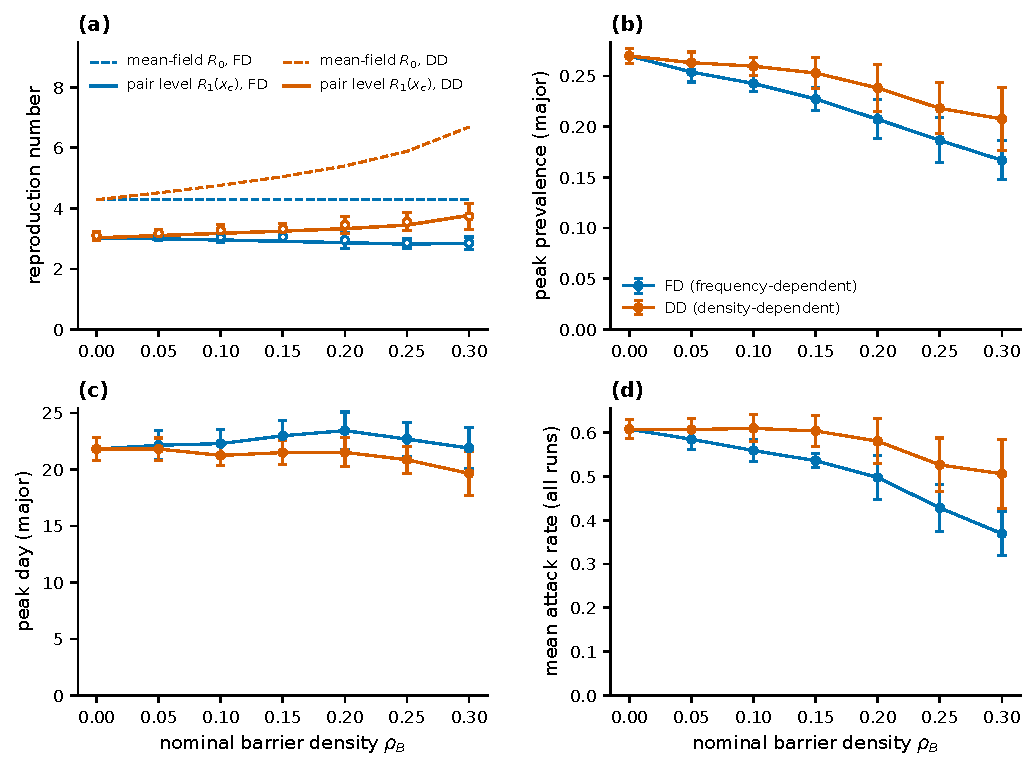
\includegraphics[width=0.86\textwidth]{fig6_3_obstacle_scan_en}
  \caption{Barrier scan with identical starts: uniform room ($20\times13$ cells, $\Npop=100$, $q=1.2$,
  $D=1\cellday$, same-cell kernel), random nested barriers at nominal density $\rho_B$; 8 layouts with 500
  epidemics per layout and density; bars are 95\,\% intervals across layouts. Blue: FD; orange: DD (pair hazard
  frozen at its barrier-free value).
  (a)~Mean-field $\Rz$ (dashed), pair-level $\Rone(x_c)$ of the centre index (solid)
  and counted $\Rhat$ of the index (open circles, 500 runs per layout with only the index transmitting).
  (b)~Peak prevalence and (c)~peak day of major outbreaks. (d)~Mean attack rate over all runs. Effects with
  layout-level standard errors, including the peak delay that panel~(c) cannot resolve, are in
  Table~\ref{s7_interventions:tab:barriers}.}
  % src: figures/fig6_3_obstacle_scan_en.pdf (code/bsc_sim/experiments/21_figures_more.py <- data/bsc_sim/06_obstacles.json)
  \label{s7_interventions:fig:barriers}
\end{figure}

\begin{table}[tbp]
  \centering\footnotesize\setlength{\tabcolsep}{3.5pt}
  \caption{Barriers with identical starts in the uniform room of Fig.~\ref{s7_interventions:fig:barriers}:
  means over 40 nested layouts (1,000 epidemics per layout and arm at $D=1$, 500 at $D=10$). $\rho_B$: nominal
  barrier density; $\Rone(x_c)$: pair-level number of the centre index; $P$: probability of a major outbreak;
  attack: mean attack rate over all runs; peak and day: peak prevalence (\%) and peak day of major outbreaks.
  The $\Delta$ columns are differences from the barrier-free arm of the same layout, mean $\pm$ standard error
  across layouts ($\Delta$peak in percentage points, $\Delta$day in days). $^{\ddagger}$Re-check:
  40 other layouts, 1,000 epidemics each, second simulator.}
  \label{s7_interventions:tab:barriers}
  % src: data/s7_interventions_tables.tex (code/s7_interventions_numbers.py) <- data/s7_interventions_barriers.json (code/s7_interventions_barriers.py); ddagger rows: code/bsc_sim/verify/v08b_obstacles_many.json
  \begin{tabular}{@{}cccccccccccc@{}}
    \toprule
    $D$ & law & $\rho_B$ & $\Rz$ & $\Rone(x_c)$ & $P$ & attack & peak & day & $\Delta$attack & $\Delta$peak & $\Delta$day \\
    \midrule
    1 & FD & 0.00 & 4.29 & 3.02 & 0.698 & 0.609 & 27.2 & 21.5 & -- & -- & -- \\
    1 & FD & 0.10 & 4.29 & 2.94 & 0.688 & 0.569 & 24.7 & 22.3 & $-0.040\pm0.003$ & $-2.5\pm0.1$ & $+0.81\pm0.12$ \\
    1 & FD & 0.30 & 4.29 & 2.80 & 0.625 & 0.386 & 17.6 & 22.4 & $-0.223\pm0.011$ & $-9.6\pm0.4$ & $+0.93\pm0.23$ \\
    1 & DD & 0.10 & 4.76 & 3.16 & 0.713 & 0.608 & 26.4 & 21.2 & $-0.001\pm0.004$ & $-0.8\pm0.1$ & $-0.33\pm0.12$ \\
    1 & DD & 0.30 & 6.68 & 3.69 & 0.727 & 0.524 & 22.0 & 20.3 & $-0.085\pm0.015$ & $-5.2\pm0.5$ & $-1.22\pm0.25$ \\
    1 & FD$^{\ddagger}$ & 0.10 & 4.29 & -- & 0.683 & 0.564 & 24.6 & 22.3 & $-0.047\pm0.004$ & $-2.4\pm0.1$ & $+0.82\pm0.10$ \\
    1 & FD$^{\ddagger}$ & 0.30 & 4.29 & -- & 0.627 & 0.376 & 17.0 & 22.2 & $-0.235\pm0.011$ & $-10.0\pm0.3$ & $+0.71\pm0.30$ \\
    \midrule
    10 & FD & 0.00 & 4.29 & 3.90 & 0.757 & 0.744 & 44.0 & 14.3 & -- & -- & -- \\
    10 & FD & 0.10 & 4.29 & 3.87 & 0.764 & 0.749 & 43.2 & 14.7 & $+0.005\pm0.005$ & $-0.8\pm0.1$ & $+0.34\pm0.05$ \\
    10 & FD & 0.30 & 4.29 & 3.75 & 0.743 & 0.719 & 38.7 & 16.4 & $-0.025\pm0.005$ & $-5.3\pm0.3$ & $+2.05\pm0.16$ \\
    10 & DD & 0.10 & 4.76 & 4.25 & 0.779 & 0.770 & 46.2 & 13.3 & $+0.026\pm0.005$ & $+2.2\pm0.1$ & $-1.05\pm0.05$ \\
    10 & DD & 0.30 & 6.68 & 5.47 & 0.826 & 0.821 & 48.8 & 11.5 & $+0.077\pm0.005$ & $+4.8\pm0.6$ & $-2.78\pm0.21$ \\
    \bottomrule
  \end{tabular}
\end{table}

\subsection{Occupancy}\label{s7_interventions:sec:occupancy}

In the office scene we vary the number of people from $\Npop=20$ to $400$ (0.03 to 0.68 persons per m$^2$;
2,000 epidemics per point; Fig.~\ref{s7_interventions:fig:occupancy}).
% src: data/bsc_sim/07_occupancy.json (density_per_m2, n_rep)
 Under FD the mean-field $\Rz$ does not
depend on $\Npop$ at all: it is $5.11$ ($\Dz=1$) and $4.68$ ($\Dz=10$) for every occupancy. Discrete people do
feel occupancy, through saturation: with fewer people an infective exhausts its neighbours sooner. At $\Dz=1$
the counted $\Rhat$ is $1.47\pm0.04$ for $\Npop=50$, $2.29\pm0.05$ for $100$ and $3.70\pm0.09$ for $400$, following
$\Ronebar=1.52$, $2.27$, $3.65$; the attack rate of major outbreaks is 27\,\%, 46\,\% and 90\,\%. At $\Dz=10$
the dependence is weaker ($\Rhat=3.2$, $3.8$, $4.5$). The elasticity of $\Ronebar$ with respect to $\Npop$
near $\Npop=100$ (between 75 and 150) is $+0.48$ at $\Dz=1$ and $+0.17$ at $\Dz=10$, against $0$ for $\Rz$.
% src: data/bsc_sim/07_occupancy.json keys D0=1|N=50|FD, N=100, N=400, D0=10|... (R0_ngm, R1_pair_uniform, R_index_alone, R_index_alone_se, attack_major_mean); elasticities: data/s7_interventions_numbers.json occupancy/elasticity|D0=1|FD, D0=10|FD (pair)
Under DD (reference $\Npop=100$), $\Rz$ is proportional to $\Npop-1$ by \eqref{M-s7_interventions:eq:dd}, from
$0.98$ at $\Npop=20$ to $20.6$ at $\Npop=400$ for $\Dz=1$, and the elasticity is $+1.0$ at both mobilities.
Halving the office from 100 to 50 people then takes $\Ronebar$ from $2.27$ to $1.12$ and the outbreak
probability from $0.49$ to $0.27$ at $\Dz=1$ ($3.79\to1.88$ and $0.74\to0.53$ at $\Dz=10$), whereas under FD it
takes them to $1.52$ and $0.40$ ($3.22$ and $0.72$).
% src: data/bsc_sim/07_occupancy.json keys D0=1|N=20|DD, N=400|DD, N=50|DD, N=50|FD, N=100|FD and the D0=10 analogues (R0_ngm, R1_pair_uniform, p_major)

Whether a capacity limit works is therefore an \emph{assumption about contact behaviour} --- do people keep
the same number of contacts in an emptier room? --- and not an output of the model.

\begin{figure}[tbp]
  \centering
  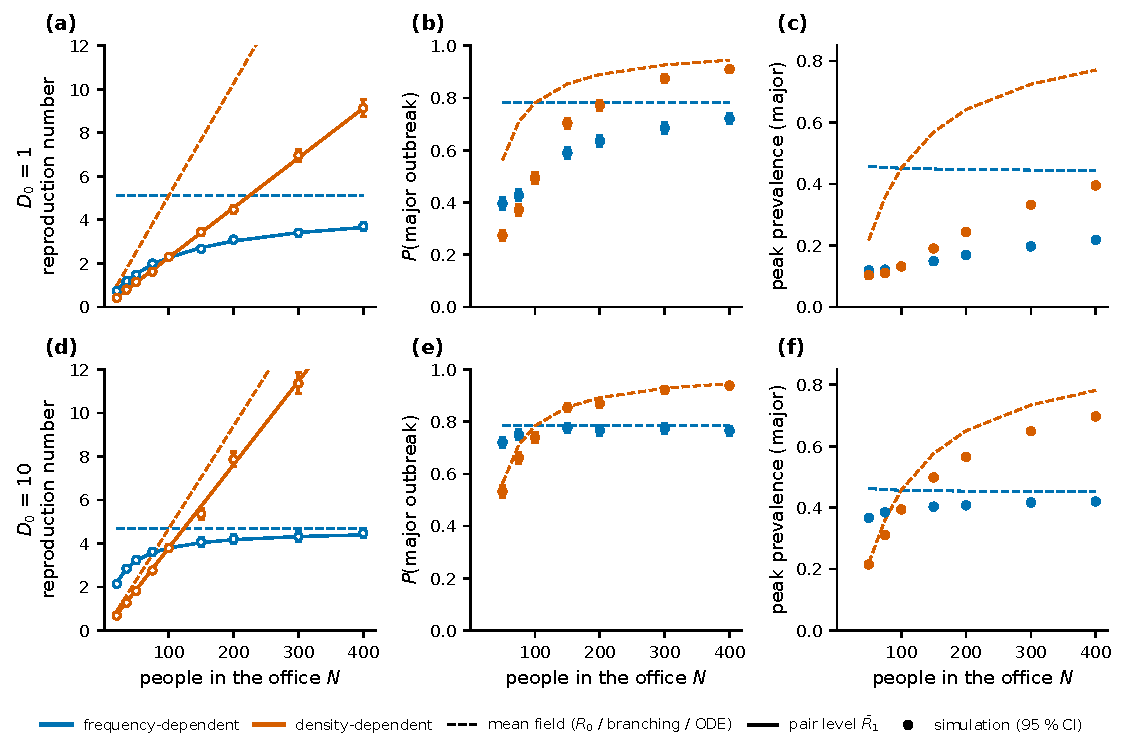
\includegraphics[width=\textwidth]{fig6_4_occupancy_en}
  \caption{Occupancy dependence in the office scene (1\,m kernel, 2,000 epidemics per point), $\Dz=1$ (top) and
  $\Dz=10$ (bottom). Blue: FD; orange: DD with the pair hazard frozen at its value for $\Npop=100$.
  (a,\,d)~Mean-field $\Rz$ (dashed), pair-level $\Ronebar$ (solid) and counted
  $\Rhat$ (open circles, 95\pct{} intervals). (b,\,e)~Probability of a major outbreak: simulation (dots, 95\,\%
  intervals) and mean-field branching value (dashed); for $\Npop<50$ a `major' outbreak means two or three
  cases. (c,\,f)~Peak prevalence of major outbreaks: simulation (dots) and lattice mean-field equations
  \eqref{M-s2_model:eq:meanfield} (dashed).}
  % src: figures/fig6_4_occupancy_en.pdf (code/bsc_sim/experiments/21_figures_more.py <- data/bsc_sim/07_occupancy.json)
  \label{s7_interventions:fig:occupancy}
\end{figure}

\subsection{Interventions}\label{s7_interventions:sec:measures}

Table~\ref{s7_interventions:tab:interventions} applies five measures to the office scene. Two of them are
\emph{inputs}, not results: `ventilation' halves $q$ in every cell and `masks' multiply $\beta$ by $0.3$, by
assumption.

\emph{Uniform measures} scale $\Rz$ exactly ($5.11\to2.55$ and $1.53$ at $\Dz=1$), but the pair-level number
less than proportionally ($\Ronebar=2.27\to1.51$ and $1.05$), because a lower hazard also wastes fewer
contacts; the outbreak probability falls from $0.49$ to $0.30$ and $0.15$. \emph{Halving the occupancy}
leaves $\Rz$ unchanged under FD and halves it under DD (Section~\ref{s7_interventions:sec:occupancy}); in
either case the peak comes earlier, on day 13 instead of day 24 at $\Dz=1$, because a smaller group is
exhausted sooner. \emph{Partitions} (39 workstation cells turned
into barriers) leave $\Rz$ at $5.11$ under FD and raise it to $6.14$ under DD at $\Dz=1$; the mean attack rate
falls from $0.232$ to $0.166$ (FD) or $0.195$ (DD). At $\Dz=10$ it goes from $0.737$ to $0.693$ (FD) or $0.751$
(DD); the decrease of $\Rz$ under FD there ($4.68\to4.63$, $-1.1\pct$) arises because the cells removed have
an above-average $q$ (Section~\ref{M-s4_geometry:sec:examples}).
% src: data/bsc_sim/08_interventions.json keys office|D0=1|... and office|D0=10|... (R0_ngm, R1_pair_uniform, p_major, peak_time_major_mean, attack_all_mean)

\emph{Combination} (ventilation, half occupancy and partitions together). At $\Dz=1$, $\Rz=2.56$ (FD) or $1.52$
(DD), $\Ronebar=1.10$ or $0.82$ and $\Rhat=1.09\pm0.03$ or $0.78\pm0.02$; at $\Dz=10$, $\Ronebar=1.79$ or
$1.16$. In the classroom the combination gives $\Ronebar=1.21$ (FD) or $0.86$ (DD) at $\Dz=1$ and $1.70$ or
$1.10$ at $\Dz=10$.
% src: data/bsc_sim/08_interventions.json keys office|D0=1|combination|FD, |DD, office|D0=10|combination|FD, |DD, classroom|D0=1|combination|FD, |DD, classroom|D0=10|combination|FD, |DD
A pair-level number below one is reached only for discrete people at low mobility under the DD law, and it
must not be read as a control criterion: in that arm $\Rz$ is $1.52$ and 16.5\,\% of the runs still reach an
attack rate of 10\,\% (five of 50 people), and conversely a pair-level number above one does not imply
outbreaks (Remark~\ref{M-s5_pair:rem:threshold}).
% src: data/bsc_sim/08_interventions.json key office|D0=1|combination|DD (p_major = 0.165)

\emph{Targeted ventilation.} Halving $q$ on the quarter of the cells with the largest elasticity $e_x$
(Theorem~\ref{M-s4_geometry:thm:hotspots}) lowers $\Rz$ more than treating the quarter with the smallest ($4.67$
against $5.11$ at $\Dz=1$; $4.10$ against $4.37$ at $\Dz=10$). For discrete people at $\Dz=1$ it makes no
measurable difference which quarter is treated: $\Ronebar=2.08$, $2.09$ and $2.06$ and mean attack rates
$0.195$, $0.205$ and $0.188$ (standard errors about $0.005$) for the hottest quarter, the coldest quarter and the hottest
quarter by the pair-level elasticity; at $\Dz=10$ the attack rates are $0.675$, $0.696$ and $0.682$.
% src: data/bsc_sim/08_interventions.json keys office|D0=1|hotspot ventilation (25 % of cells)|FD, coldspot ..., pair-level hotspot ..., and D0=10 (R0_ngm, R1_pair_uniform, attack_all_mean, attack_all_sd/sqrt(2000))

\begin{table}[tbp]
  \centering\footnotesize\setlength{\tabcolsep}{4pt}
  \caption{Interventions in the office scene (1\,m kernel; 2,000 epidemics per arm; reference occupancy for DD:
  $\Npop=100$ in the unmodified scene). $\Rhat$: counted secondary cases of the index ($\pm$ standard error);
  $P$: probability of a major outbreak; attack: mean attack rate over all runs; peak and day: peak prevalence
  (\%) and peak day of major outbreaks. Ventilation and masks are assumptions on $q$ and $\beta$, not model
  outputs. Partitions: 39 workstation cells turned into barriers. Combination: ventilation, half occupancy and
  partitions. A value $\Ronebar<1$ is not a control criterion (see text).}
  \label{s7_interventions:tab:interventions}
  % src: data/s7_interventions_tables.tex (code/s7_interventions_numbers.py) <- data/bsc_sim/08_interventions.json
  \begin{tabular}{@{}cllcccccccc@{}}
    \toprule
    $\Dz$ & measure & law & $\Npop$ & $\Rz$ & $\Ronebar$ & $\Rhat$ & $P$ & attack & peak & day \\
    \midrule
    1 & baseline & FD & 100 & 5.11 & 2.27 & $2.30\pm0.05$ & 0.491 & 0.232 & 12.8 & 24.3 \\
    1 & ventilation, $q\to q/2$ & FD & 100 & 2.55 & 1.51 & $1.55\pm0.04$ & 0.295 & 0.102 & 9.0 & 23.3 \\
    1 & masks, $\beta\to0.3\beta$ & FD & 100 & 1.53 & 1.05 & $1.05\pm0.03$ & 0.147 & 0.048 & 7.1 & 21.8 \\
    1 & capacity 50\,\% & FD & 50 & 5.11 & 1.52 & $1.51\pm0.04$ & 0.393 & 0.126 & 11.7 & 13.0 \\
    1 & capacity 50\,\% & DD & 50 & 2.53 & 1.12 & $1.13\pm0.03$ & 0.258 & 0.080 & 10.2 & 13.9 \\
    1 & partitions & FD & 100 & 5.11 & 2.21 & $2.20\pm0.05$ & 0.459 & 0.166 & 10.7 & 20.3 \\
    1 & partitions & DD & 100 & 6.14 & 2.42 & $2.36\pm0.06$ & 0.506 & 0.195 & 11.4 & 19.9 \\
    1 & combination & FD & 50 & 2.56 & 1.10 & $1.09\pm0.03$ & 0.274 & 0.077 & 9.9 & 12.2 \\
    1 & combination & DD & 50 & 1.52 & 0.82 & $0.78\pm0.02$ & 0.165 & 0.055 & 9.0 & 12.3 \\
    \midrule
    10 & baseline & FD & 100 & 4.68 & 3.79 & $3.76\pm0.09$ & 0.760 & 0.737 & 39.0 & 16.7 \\
    10 & ventilation, $q\to q/2$ & FD & 100 & 2.34 & 2.09 & $2.09\pm0.06$ & 0.522 & 0.404 & 21.2 & 27.6 \\
    10 & masks, $\beta\to0.3\beta$ & FD & 100 & 1.40 & 1.30 & $1.30\pm0.04$ & 0.290 & 0.131 & 10.9 & 27.8 \\
    10 & capacity 50\,\% & FD & 50 & 4.68 & 3.22 & $3.20\pm0.07$ & 0.697 & 0.629 & 36.2 & 15.8 \\
    10 & capacity 50\,\% & DD & 50 & 2.31 & 1.88 & $1.85\pm0.05$ & 0.533 & 0.345 & 21.6 & 19.3 \\
    10 & partitions & FD & 100 & 4.63 & 3.60 & $3.60\pm0.09$ & 0.730 & 0.693 & 34.2 & 19.6 \\
    10 & partitions & DD & 100 & 5.55 & 4.14 & $4.13\pm0.10$ & 0.777 & 0.751 & 38.0 & 17.0 \\
    10 & combination & FD & 50 & 2.31 & 1.79 & $1.74\pm0.05$ & 0.504 & 0.285 & 18.8 & 19.5 \\
    10 & combination & DD & 50 & 1.37 & 1.16 & $1.19\pm0.04$ & 0.329 & 0.123 & 12.6 & 16.7 \\
    \bottomrule
  \end{tabular}
\end{table}

\subsection{Schedules and dwell time}\label{s7_interventions:sec:time}

\begin{proposition}[Duty cycle]\label{s7_interventions:prop:duty}
  Let $0<f\le1$ and let Assumption~\ref{M-s2_model:ass:A} hold. Suppose that movement and transmission operate
  only during the occupied intervals $[k,k+f)$, $k=0,1,2,\dots$ (time in days), and that recovery proceeds at all
  times: in \eqref{M-s2_model:eq:meanfield}, $\gen$ and $\Fm$ are multiplied by $\chi(t)$, equal to $1$ on the
  occupied intervals and to $0$ otherwise. Put $\theta(t)=\int_0^t\chi(s)\,\dd s$ and
  \begin{equation}\label{s7_interventions:eq:dutydetail}
    \Jm_f=\gen+\Fm-\frac{\gamma}{f}\,\Id,\qquad \Rz^{(f)}=\srad\Bigl(\Fm\bigl(\tfrac{\gamma}{f}\,\Id-\gen\bigr)^{-1}\Bigr).
  \end{equation}
  \begin{enumerate}
    \item[(a)] The linearised model $\dot I=[\chi(t)(\gen+\Fm)-\gamma\Id]\,I$ has the solution
      $I(t)=\exp[\theta(t)(\gen+\Fm)-\gamma t\,\Id]\,I(0)$; in particular $I(k)=\e^{kf\Jm_f}I(0)$ for integer $k$.
      Solutions of the nonlinear model satisfy $I(t)\le\exp[\theta(t)(\gen+\Fm)-\gamma t\,\Id]\,I(0)$ componentwise.
    \item[(b)] The growth factor per day is $\e^{f\sabs(\Jm_f)}$, and $\sabs(\Jm_f)$ has the sign of $\Rz^{(f)}-1$.
    \item[(c)] If $\gen=\Dz\genz$ and $\Rz(\Dz)$ denotes the value for continuous occupancy, then
      $\Rz^{(f)}(\Dz)=f\,\Rz(f\Dz)$. For the same-cell kernel,
      $f\,\Rz(\Dz)\le\Rz^{(f)}(\Dz)\le f\beta\qmax/\gamma$.
  \end{enumerate}
\end{proposition}
\begin{proof}
  (a) The matrices $A(t)=\chi(t)(\gen+\Fm)-\gamma\Id$ are constant on each occupied and each empty interval and
  commute with one another for all times, so the product of the exponentials over successive intervals is the
  exponential of $\int_0^tA(s)\,\dd s=\theta(t)(\gen+\Fm)-\gamma t\,\Id$; at $t=k$, $\theta=kf$. In the nonlinear
  model $S_y\le N^*_y$ gives $\dot I\le A(t)I$ componentwise, and since $A(t)$ is Metzler the comparison
  argument of Theorem~\ref{M-s3_r0:thm:ngm}(d) applies on each interval.
  (b) $\gen+\Fm$ is Metzler and irreducible, so $\e^{f\Jm_f}$ is a positive matrix with spectral radius
  $\e^{f\sabs(\Jm_f)}$ (Lemma~\ref{s3_r0:lem:facts}, P1); the sign statement is Theorem~\ref{M-s3_r0:thm:ngm}(c) with
  $\gamma$ replaced by $\gamma/f$.
  (c) $\Fm\bigl(\tfrac{\gamma}{f}\Id-\Dz\genz\bigr)^{-1}=f\,\Fm(\gamma\Id-f\Dz\genz)^{-1}$. The inequalities follow
  from Theorem~\ref{M-s3_r0:thm:mobility}(c), because $f\Dz\le\Dz$, and from Theorem~\ref{M-s3_r0:thm:bounds}.
\end{proof}

\begin{remark}[What is exact and what is approximate]\label{s7_interventions:rem:duty}
  $\Rz^{(f)}$ is an exact threshold parameter of the periodic mean-field model, for any cycle length, because
  one and the same operator is switched on and off; in general periodic models the threshold is given by a
  next-generation operator on periodic functions and not by time-averaged parameters
  \citep{bacaer2006epidemic,wang2008threshold}. By part~(c) a duty cycle does more than scale $\Rz$ by $f$: it
  also lowers the effective mobility to $f\Dz$.
  As a \emph{number of secondary cases}, however, the substitution $\gamma\to\gamma/f$ is an approximation. It
  replaces the expected infectious time spent in the room by $f/\gamma$ ($2.381$ days for $f=1/3$), whereas a
  case that becomes infectious at the start of an occupied interval spends
  $(1-\e^{-\gamma f})/[\gamma(1-\e^{-\gamma})]=2.493$ days there ($+4.7\,\%$), and one that becomes infectious
  at a uniformly distributed time within an occupied interval, as secondary cases approximately do (their
  infection times within an interval follow the incidence, which changes during the interval), $2.383$ days
  ($+0.07\,\%$).
  % src: data/s7_interventions_schedule.json keys duty|office|D0=1 (in_room_time_rule, in_room_time_start, in_room_time_uniform); closed forms in code/s7_interventions_schedule.py
  For discrete individuals the same substitution in the pair-level formulas of Section~\ref{M-s5_pair:sec} is
  likewise an approximation. The exact pair-level value follows from the argument of
  Proposition~\ref{M-s5_pair:prop:pair}. Let $A=\gamma\Id+\mathbf{H}-\mathcal{M}^{\T}$ be the pair operator of
  that proposition and $u_0(z)$ the probability that the given person escapes infection when the index case
  becomes infectious at the start of an occupied interval with the pair in state $z$. During the occupied
  interval of length $f$ the pair moves and the hazard acts, so $(\e^{-At}\one)(z)$ is the probability that
  neither recovery nor infection has occurred by time $t\le f$; during the rest of the day nobody moves, the
  index recovers with probability $c_f=1-\e^{-\gamma(1-f)}$, and otherwise the next day starts from the same
  state. Hence
  \begin{equation}\label{s7_interventions:eq:dutyexact}
    u_0=\gamma A^{-1}\bigl(\one-\e^{-Af}\one\bigr)+\e^{-Af}\bigl(c_f\,\one+(1-c_f)\,u_0\bigr),
  \end{equation}
  a linear fixed-point equation whose map is a contraction in the maximum norm (factor at most
  $\e^{-\gamma}<1$, because $\e^{-Af}$ is non-negative with row sums at most $\e^{-\gamma f}$), solved by
  iteration; the expected number of secondary cases is $(\Npop-1)$ times the mean of $1-u_0$ over the
  $\ncell^2$ pair states. For an index case that becomes infectious at a time uniformly distributed over the
  occupied interval, the first day is shortened to its remaining part $r$ and the same expression is averaged
  over $r\in(0,f)$. With $f=1$ the iteration reproduces the solution of \eqref{M-s5_pair:eq:pair} to
  $5\times10^{-10}$.
  % src: code/s7_interventions_schedule.py (duty_cycle_exact); data/s7_interventions_schedule.json key duty_exact|control_f1|office|D0=1 (abs_diff 4.6e-10), duty_exact|office|D0=1 (fixed_point_residual 9e-13, 152 iterations)
\end{remark}

\paragraph{Office, eight hours a day ($f=1/3$).} The mean-field number drops from $5.11$ to
$\Rz^{(f)}=1.75$ at $\Dz=1$ and from $4.68$ to $1.60$ at $\Dz=10$; the pair-level number with
$\gamma\to\gamma/f$ is $\Ronebar=0.889$ and $1.335$ (Table~\ref{M-s7_interventions:tab:dwell}a). The exact
pair-level values of \eqref{s7_interventions:eq:dutyexact} are $0.930$ at $\Dz=1$ and $1.397$ at $\Dz=10$ for
an index case that becomes infectious at the start of a working day, $4.6\pct$ and $4.7\pct$ above the rule,
as its longer time in the room leads one to expect, and $0.889$ and $1.336$ for one that becomes infectious
at a uniformly distributed time of the working day, $0.07\pct$ above the rule.
% src: data/s7_interventions_schedule.json keys duty_exact|office|D0=1, duty_exact|office|D0=10 (exact_start 0.9296, 1.3975; exact_uniform_phase 0.8892, 1.3359; rule_gamma_over_f 0.8885, 1.3349; start_over_rule_pct 4.62, 4.69; uniform_over_rule_pct 0.07), duty|office|D0=1, D0=10 (R0_duty)
Simulation with the schedule imposed explicitly agrees: $0.9309\pm0.0009$ and $0.8889\pm0.0009$ at $\Dz=1$
(2{,}000{,}000 runs each) and $1.400\pm0.002$ and $1.337\pm0.002$ at $\Dz=10$ (800{,}000 runs each), all
within $1.6$ standard errors of the exact values.
% src: data/s7_interventions_schedule.json keys duty_large|office|D0=1, duty_large|office|D0=10 (count_start, count_start_se, count_uni, count_uni_se, z_start 1.52 and 1.26, z_uni -0.33 and 0.82); smaller samples are listed below
In full epidemics with the schedule, 6.1\pct{} of the runs (95\pct{} interval 5.1--7.2\pct) reach a 10\pct{} attack
rate at $\Dz=1$ and 30.2\pct{} (28.2--32.2\pct) at $\Dz=10$. The index case of an office occupied eight hours a
day thus infects about $0.9$ people on average at $\Dz=1$ and $1.3$ to $1.4$ at $\Dz=10$, against $2.3$ and
$3.8$ for a room occupied around the clock; this is not a threshold statement
(Remark~\ref{M-s5_pair:rem:threshold}).
% src: data/bsc_sim/11_dwell_time.json keys office|D0=1, office|D0=10 (p_major, p_major_lo, p_major_hi)
For a class that meets one hour a day ($f=1/24$) the numbers are $\Rz^{(f)}=0.27$, $\Ronebar=0.18$ with the
rule and $0.194$ exactly (index infectious from the start of the lecture; counted $0.189\pm0.003$) at
$\Dz=1$, and no run in 2,000 reaches a 10\pct{} attack rate: with $\beta=0.5\perday$ one daily lecture cannot
sustain transmission in this model.
% src: data/bsc_sim/11_dwell_time.json key classroom|D0=1 (R0_duty_cycle, R1_pair_duty_cycle, sim_R_schedule, p_major); data/s7_interventions_schedule.json key duty_exact|classroom|D0=1 (exact_start 0.1944)

\paragraph{Further simulation estimates of the duty-cycle counts.} Before the exact values of
\eqref{s7_interventions:eq:dutyexact} were computed, the number of secondary cases of an index case in the
office occupied eight hours a day was estimated by simulation several times. For an index case infectious
from the start of a working day at $\Dz=1$: $0.918\pm0.009$ (one batch of 20,000 runs), $0.944\pm0.006$ (the
second simulator), $0.928\pm0.003$ (pooled, in the re-check's report) and $0.935\pm0.003$ (200,000
runs), against the exact $0.930$; at $\Dz=10$, $1.408\pm0.012$ and $1.395\pm0.004$ against $1.397$. For an
index case infectious from a uniformly distributed time: $0.896\pm0.003$ and $1.331\pm0.004$ (200,000 runs
each) against $0.889$ and $1.336$. The 200,000-run samples at $\Dz=1$ lie $2.0$ and $2.5$ standard errors
above the exact values; the samples of 2,000,000 runs quoted in Section~\ref{s7_interventions:sec:time} do
not ($+1.5$ and $-0.3$).
% src: data/bsc_sim/11_dwell_time.json keys office|D0=1, office|D0=10 (sim_R_schedule and its interval); code/bsc_sim/verify/v11.json key office_duty_D1; data/checks/simulation.json: duty_cycle_office_D0_1.count_explicit_schedule_pooled (0.928 +- 0.003), .first_analysis_batch (0.918) (notes/VERIFICATION.md Section 4.2, simulations item 11); data/s7_interventions_schedule.json keys duty|office|D0=1, D0=10 (count_start, count_uniform_phase and their se), duty_exact|office|D0=* (z_mc_start 1.97, z_mc_uniform_phase 2.54), duty_large|office|D0=1 (z_start 1.52, z_uni -0.33)

\paragraph{One visit.} Table~\ref{M-s7_interventions:tab:dwell}b gives the expected number of people that one
infective infects during a single stay of length $T$. For a uniformly placed infective the mean-field value is
$\beta\langle q\rangle(1-\e^{-\gamma T})/\gamma$ whatever the mobility and the kernel, because the walk is
stationary; the counted exposure agrees with it within 0.3\,\%, and the counted infections are lower only
where pairs saturate within the visit. The values are $0.21$ for an office day ($0.175$ counted at $\Dz=1$,
$0.198$ at $\Dz=10$), $0.027$ for a lecture, $0.018$ for a 20-minute metro ride and $0.0086$ for a 27-minute
supermarket visit.
% src: data/bsc_sim/11_dwell_time.json keys <scene>|D0=1, <scene>|D0=10 (per_visit_meanfield, per_visit_sim, per_visit_exposure_sim; 200,000 runs each)
A per-visit number is not the reproduction number of a setting that is visited repeatedly: an infective who
rides the metro twice a day for the whole infectious period infects $f\beta\langle q\rangle/\gamma=0.25$
fellow passengers in expectation, and one who shops once a day $0.06$ fellow customers. Weighting each
setting by the fraction of time spent in it is the residence-time (Lagrangian) formulation of multi-setting
epidemic models \citep{bichara2015sis}; here it is applied to one setting at a time. These numbers, and
not the closed-room values, are what the settings contribute, and they undercut the ranking of
Section~\ref{M-s6_scenes:sec}: as closed rooms the scenes rank metro, classroom, office, supermarket
($\Rz=9.2$, $5.9$, $5.1$, $4.4$ at $\Dz=1$); with the dwell times above the mean-field numbers are $1.75$ for
the office and $0.27$ for the lecture ($\Rz^{(f)}$, closed groups), $0.25$ for the metro carriage and $0.06$
for the supermarket ($f\beta\langle q\rangle/\gamma$).
% src: data/bsc_sim/11_dwell_time.json (wellmixed_duty_cycle: metro 0.2515, supermarket 0.0612; R0_continuous; R0_duty_cycle)

\paragraph{A daily schedule of the parameters.} In the metro scene we let the mobility field and a transmission
multiplier follow a daily signal with two rush hours (24 hourly segments; the multiplier is $1$ in the rush
hours and $0.8$ otherwise, mean $0.833$), and compare three arms: constant rush-hour values (the scene of
Section~\ref{M-s6_scenes:sec}), the hourly schedule, and constants equal to the time averages of the mobility
field and of the multiplier. The number of people is $\Npop=310$ in all arms: only mobility and the multiplier
vary, not the occupancy.
% src: code/bsc_sim/experiments/09_metro_time.py; data/bsc_sim/09_metro_time.json key schedule (m_mean)

\begin{observation}[Time average]\label{s7_interventions:obs:average}
  In the metro scene the hourly schedule and its time average give the same outbreak probability, attack
  rate, peak prevalence and peak day within Monte Carlo error at $\Dz=1$, $10$ and $100$
  (Table~\ref{s7_interventions:tab:schedule}); for example the peak prevalence of
  major outbreaks is 23.0\pct{} against 22.9\pct{} on day 25.3 against 25.2 at $\Dz=1$.
\end{observation}
% src: data/bsc_sim/09_metro_time.json keys D0=1|varying, D0=1|mean, D0=100|...; data/s7_interventions_schedule.json keys metro|D0=10|peak, varying, mean
A test in the re-check, run with the production simulator, in the office scene (half of each day with hop rates multiplied by $1.8$
and transmission by $1.3$, the other half by $0.2$ and $0.7$, against constants; 6,000 epidemics each) agrees:
outbreak probability $0.491$ against $0.498$, peak prevalence 12.8\,\% against 12.8\,\%, peak day $23.7$ against
$23.3$ (standard error $0.3$).
% src: code/bsc_sim/verify/v14_schedule.json keys check_varying, check_mean
This is not a theorem: the hourly generators do not commute and the hop rates are not small compared with one
cycle per day. Relative to constant rush-hour values the schedule lowers the multiplier but raises the
mobility; the first effect wins at $\Dz=1$ (peak 25.0\,\% $\to$ 23.0\,\%, three days later), the second at
$\Dz=100$ (35.4\,\% $\to$ 44.2\,\%, 2.6 days earlier), and at $\Dz=10$ they nearly cancel.

\begin{table}[tbp]
  \centering\footnotesize\setlength{\tabcolsep}{5pt}
  \caption{Daily schedule in the metro scene ($\Npop=310$ in every arm, 1\,m kernel, FD, 2,000 epidemics per
  arm). Arms: constant rush-hour values (`peak'), hourly schedule of mobility and transmission multiplier
  (`schedule'), constants equal to the time averages (`average'). $\Rz$ is not defined by a single matrix
  for the schedule arm. 95\,\% intervals in parentheses.}
  \label{s7_interventions:tab:schedule}
  % src: data/s7_interventions_tables.tex (code/s7_interventions_numbers.py) <- data/bsc_sim/09_metro_time.json (D0 = 1, 100); data/s7_interventions_schedule.json (D0 = 10)
  \begin{tabular}{@{}clccccc@{}}
    \toprule
    $\Dz$ & arm & $\Rz$ & $P(\text{major})$ & attack, major (\%) & peak prevalence, major (\%) & peak day, major \\
    \midrule
    1 & peak & 9.24 & 0.871 (0.855--0.885) & 93.6 & 25.0 (24.7--25.2) & 22.2 (21.6--22.7) \\
    1 & schedule & -- & 0.837 (0.820--0.853) & 93.4 & 23.0 (22.7--23.2) & 25.3 (24.6--26.0) \\
    1 & average & 7.66 & 0.844 (0.827--0.859) & 93.7 & 22.9 (22.7--23.1) & 25.2 (24.5--25.9) \\
    \midrule
    10 & peak & 9.16 & 0.887 (0.873--0.901) & 97.9 & 27.8 (27.5--28.1) & 21.0 (20.5--21.5) \\
    10 & schedule & -- & 0.869 (0.854--0.883) & 99.3 & 28.6 (28.3--28.9) & 21.0 (20.5--21.4) \\
    10 & average & 7.58 & 0.862 (0.846--0.876) & 99.3 & 28.6 (28.4--28.9) & 20.9 (20.5--21.4) \\
    \midrule
    100 & peak & 9.08 & 0.880 (0.866--0.894) & 99.9 & 35.4 (35.1--35.8) & 16.5 (16.2--16.8) \\
    100 & schedule & -- & 0.853 (0.836--0.867) & 99.8 & 44.2 (43.9--44.6) & 13.9 (13.7--14.1) \\
    100 & average & 7.55 & 0.855 (0.839--0.870) & 99.8 & 44.4 (44.0--44.7) & 13.9 (13.8--14.1) \\
    \bottomrule
  \end{tabular}
\end{table}

\subsection{What remains at higher mobility}\label{s7_interventions:sec:regime}

The experiments above were run at $\Dz=1$ and $10$. The pair-level number $\Ronebar$ is exact for the first
generation at any mobility (Definition~\ref{M-s5_pair:def:R1}) and costs one linear solve, so each effect can be
followed up to $\Dz=2.4\times10^{3}\cellday$, the estimate of Section~\ref{M-s2_model:sec:regime} for people who
walk 5\pct{} of the time (Table~\ref{s7_interventions:tab:regime}). The effects
of the contrast in $q$ and of
barriers under FD shrink below 1\,\% at $\Dz=100$ and below 0.05\,\% at $\Dz=2.4\times10^{3}$. Simulation at
$\Dz=100$ agrees: the contrast $c=0.583$ changes the mean attack rate from $0.744$ to $0.750$ (2,000 epidemics each,
standard error $0.009$), and barriers at 10\,\% and 30\,\% change it by $+0.007\pm0.005$ and $+0.013\pm0.007$
(20 layouts with 250 epidemics each, FD).
% src: data/s7_interventions_regime.json keys det/* (R0, R1bar) and sim/twozone|D0=100|c=0.0000, c=0.5833 (attack_all_mean, attack_all_sd/sqrt(2000)), sim/barriers|D0=100|FD/paired (attack); code/s7_interventions_regime.py
Three things survive. Uniform reductions of $q$ or $\beta$ act on $\Ronebar$ almost in proportion, as they do
on $\Rz$. Occupancy matters in full under DD; under FD a residue of about 5\,\% remains for halving the office,
which is a finite-population effect (the limit $D\to\infty$ in Proposition~\ref{M-s5_pair:prop:torus}) and not a
spatial one. And the
time spent in the room enters through Proposition~\ref{s7_interventions:prop:duty} at any mobility. Epidemics
at $\Dz=2.4\times10^{3}$ were not simulated.

\begin{table}[tbp]
  \centering\footnotesize\setlength{\tabcolsep}{5pt}
  \caption{Relative change (\%) of deterministic reproduction numbers caused by the measures of this section,
  as a function of the mobility scale $\Dz$ (\cdunit). Two-zone room and barrier room: $\Npop=100$,
  same-cell kernel (barriers: mean over the 40 layouts of Table~\ref{s7_interventions:tab:barriers}); office
  scene: 1\,m kernel; DD reference: the unmodified room. Last row: the ratio $\Ronebar/\Rz$ in the office scene.}
  \label{s7_interventions:tab:regime}
  % src: data/s7_interventions_tables.tex (code/s7_interventions_numbers.py) <- data/s7_interventions_regime.json key det
  \begin{tabular}{@{}llcccc@{}}
    \toprule
    measure & quantity & $\Dz=1$ & $10$ & $100$ & $2.4\times10^{3}$ \\
    \midrule
    two-zone contrast $c=0.58$ & $\Rz$ & $+16.0$ & $+3.3$ & $+0.4$ & $+0.01$ \\
     & $\Ronebar$ & $-14.6$ & $-4.3$ & $-0.6$ & $-0.03$ \\
    barriers, $\rho_B=0.30$, FD & $\Ronebar$ & $-7.6$ & $-4.7$ & $-0.9$ & $-0.04$ \\
    barriers, $\rho_B=0.30$, DD & $\Ronebar$ & $+20$ & $+38$ & $+50$ & $+52$ \\
    capacity 50\,\%, FD (office) & $\Ronebar$ & $-32.9$ & $-15.2$ & $-6.2$ & $-4.5$ \\
    capacity 50\,\%, DD (office) & $\Ronebar$ & $-50.5$ & $-50.5$ & $-50.5$ & $-50.5$ \\
    ventilation, $q\to q/2$ (office) & $\Ronebar$ & $-33.4$ & $-45.0$ & $-48.3$ & $-48.8$ \\
    \midrule
    office scene, baseline & $\Ronebar/\Rz$ & 0.44 & 0.81 & 0.93 & 0.95 \\
    \bottomrule
  \end{tabular}
\end{table}

\subsection{Computational cost}\label{appD_tables:sec:cost}\label{s7_interventions:sec:cost}

Table~\ref{s7_interventions:tab:cost} compares, for the
office scene, two ways of computing \emph{the same quantity}, charging Monte Carlo only for the runs needed to
reach a stated accuracy (its cost scales as accuracy$^{-2}$); times are single-core CPU times on one laptop.
% src: code/bsc_sim/experiments/10_benchmark.py (method)

One sparse factorisation of $\gamma\Id-\gen$ followed by power iteration gives $\Rz$ in 1.4 to 4.6\,ms (within
$10^{-8}$ of a dense eigen-solve). Estimating the same number to 1\,\% by a particle power method costs 8 to 9
times more at $\Dz=1$ and 113 to 133 times more at $\Dz=10$ with a vectorised NumPy estimator, and 3 and 86
times more with a compiled one; at 0.1\,\% all factors are 100 times larger. The equal-accuracy speed-up is
thus a few to about $10^2$ at 1\,\% accuracy and a few hundred to about $10^4$ at 0.1\,\%; it grows with
mobility (more hops per infectious period) and depends on the implementation by a factor of two to three.
% src: data/bsc_sim/10_benchmark.json keys D0=1, D0=10 / T1_R0_meanfield (cpu_sparse_s, abs_err_sparse, speedup_at_1pct, speedup_at_0p1pct); code/bsc_sim/verify/v12_benchmark_rerun.json (same keys; re-run of the same script); code/bsc_sim/verify/v13_bench.json (speedup_1pct, speedup_01pct; compiled estimator)
The pair-lattice solve for $\Ronebar$ (conjugate gradients on $\ncell^2=54{,}756$ unknowns, 0.07 to 0.14\,s) is
about 20 ($\Dz=1$) to 90 ($\Dz=10$) times faster than counting secondary cases to 1\,\% and agrees with the
count within 0.1 standard error.
% src: data/bsc_sim/10_benchmark.json T3_R1_discrete (cpu_pair_s, speedup_at_1pct, theory_minus_mc_in_se); code/bsc_sim/verify/v12_benchmark_rerun.json T3_R1_discrete
For whole-epidemic outputs the mean-field route is not a substitute for simulation at $\Dz=1$: the branching
value of the outbreak probability is too high by $0.28$ and the attack rate of the lattice equations by $0.55$;
no speed-up is meaningful for a biased answer. At $\Dz=10$ both biases are $0.03$, and the lattice equations
(1.5\,s) are slower than simulating to 1\,\% (0.19\,s, 33 runs). The exact simulator takes 0.5\,ms for one
office epidemic at $\Dz=1$ (5,900 events) and 5.9\,ms at $\Dz=10$.
% src: data/bsc_sim/10_benchmark.json T4_p_major (theory_bias), T5_attack_rate (theory_bias, cpu_ode_s, mc_cpu_for_1pct_s, mc_runs_for_1pct), c_core_cpu_per_run_s, events_per_run
In short, the spectral formula and the pair solve are the inexpensive ways to obtain $\Rz$ and $\Ronebar$,
and simulation is cheap enough to be the method of choice for outbreak probabilities and sizes.

\begin{table}[tbp]
  \centering\footnotesize\setlength{\tabcolsep}{4pt}
  \caption{Cost of deterministic evaluation against Monte Carlo for the same quantity (office scene,
  $\Npop=100$; single-core CPU). $\noff(x)$: offspring number \eqref{M-s3_r0:eq:offspring} of a case introduced in one
  cell; CG: conjugate gradients. Speed-up: Monte Carlo CPU time needed for a relative standard error of 1\,\%
  (an absolute standard error of 0.01 for the outbreak probability) divided by the deterministic CPU time; the
  three values for $\Rz$ are the first run, the re-check's re-run of the same script, and the
  re-check's compiled estimator; the two values for the other rows are the first run and the re-check's
  re-run; no speed-up is quoted where the deterministic value is biased. Bias: deterministic value minus
  simulated value of the individual-based model.}
  \label{s7_interventions:tab:cost}
  % src: data/bsc_sim/10_benchmark.json; code/bsc_sim/verify/v12_benchmark_rerun.json; code/bsc_sim/verify/v13_bench.json (collected in data/s7_interventions_numbers.json, key cost)
  \begin{tabular}{@{}llccccc@{}}
    \toprule
     & & \multicolumn{2}{c}{deterministic CPU} & \multicolumn{2}{c}{speed-up at equal accuracy} & bias \\
    \cmidrule(lr){3-4}\cmidrule(lr){5-6}
    quantity & deterministic method & $\Dz=1$ & $\Dz=10$ & $\Dz=1$ & $\Dz=10$ & $\Dz=1$; $10$ \\
    \midrule
    $\Rz=\srad(\ngm)$ & sparse LU, power iteration & 4.6\,ms & 1.4\,ms & 8; 9; 3 & 133; 113; 86 & none \\
    $\noff(x)$, one cell & one sparse solve & 0.27\,ms & 0.29\,ms & 35; 22 & 331; 351 & none \\
    $\Ronebar$ & CG on the pair lattice & 68\,ms & 137\,ms & 18; 22 & 85; 97 & none \\
    $P(\text{major})$ & mean-field branching & 9.4\,ms & 9.7\,ms & -- & -- & $+0.28$; $+0.03$ \\
    attack rate, major & lattice equations \eqref{M-s2_model:eq:meanfield} & 0.40\,s & 1.54\,s & -- & -- & $+0.55$; $+0.03$ \\
    \bottomrule
  \end{tabular}
\end{table}

% supp_datasets.tex -- Supplementary Section S6: the outbreak records (body only; \input by supplement.tex).
% Paths in "% src:" comments are relative to the repository root.
% Tables: the three table bodies between the markers ">>> GENERATED" / "<<< GENERATED" are written by
%   code/appB_dataset_table.py (from data/bsc_outbreaks/outbreaks.csv and data/bsc_outbreaks/tables/*.csv);
%   all other numbers of this appendix are in data/appB_dataset_numbers.json (same script).
% Figure: code/appB_dataset_fig_attack.py -> figures/appB_dataset_attack_{en,zh}.pdf.
\section{The outbreak records}\label{appB_dataset:sec}

This section documents the two datasets of outbreak records used in Section~\ref{M-s8_outbreaks:sec} of the main
text. For the first dataset, 27 records of outbreaks and exposure cohorts (Section~\ref{appB_dataset:sec:first}), it
says how they were found, what was recorded, how reliable each record is, and which numbers were digitised or
reconstructed. The second dataset, eleven records of ten outbreaks with positions, follows in
Section~\ref{appB_dataset:sec:second}.

\subsection{The first dataset: 27 records of outbreaks and exposure cohorts}\label{appB_dataset:sec:first}
% src: data/bsc_outbreaks/outbreaks.csv (27 rows); data/appB_dataset_numbers.json -> n_records

\paragraph{Search and inclusion.}
Candidate outbreaks were located by web search, with one set of queries per scene (office and call centre;
supermarket and retail; classroom and school; metro, bus, train and aircraft; restaurant; choir), and by
following the citations of the papers found. This is not a systematic review and the coverage is not
exhaustive. A record was included if (a) it is described in a peer-reviewed article or an official
surveillance report, (b) the DOI of that source is registered, and (c) the source gives at least one of: the
number of exposed people, positions at seat or zone level, the geometry of the room, the duration of exposure.
% src: code/bsc_outbreaks/scripts/build_dataset.py; data/bsc_outbreaks/sources.md
The result is 27 records from 31 sources: 5 offices and workplaces, 4 retail settings, 5 classrooms and
class-like rooms, 7 vehicle cabins, 2 restaurants, 2 choir or church events, and 2 records of large settings that
lie outside the scope of the model (a cruise ship and worker dormitories). These two are recorded for reference
only, as examples of large shared settings with long exposure that a model of one closed room does not cover, and
take part in no comparison.
% src: data/appB_dataset_numbers.json -> records_by_group, sources.n
Three records without a denominator (S3, C4, T7) and one with a reported attack rate but no transcribed
counts (T6: 54 persons aboard, 72\pct{} of the passengers ill, from the abstract) were kept as context for their
settings; like the two out-of-scope records, they take no part in any quantitative comparison.
% src: data/appB_dataset_numbers.json -> records_without_denominator (S3, C4, T7), records_with_reported_rate_but_no_counts (T6), records_with_counts (23); data/bsc_outbreaks/outbreaks.csv -> T6 (occupancy_n 54, attack_rate_reported); data/refs_search.json (manual_checks.moser1979)
No documented outbreak in a metro carriage with an exposed denominator was found; buses, a coach, a minibus,
a train cohort and one flight stand in for that scene. The supermarket has one record with denominators for
staff and customers (S1) and none with geometry, positions or dwell times.
% src: data/bsc_outbreaks/outbreaks.csv (scene groups); notes/VERIFICATION.md (Section 4.4, outbreak dataset, item 3: unverifiable)

\paragraph{What was recorded.}
Each record has 51 fields: setting, place, dates and pathogen; the sources and how each was read; type and
duration of exposure; room geometry, occupancy, ventilation and mask use; the index case; the numbers
exposed and infected, with an alternative count where sources or case definitions differ; the attack rate
with its exact (Clopper--Pearson) 95\,\% interval; the spatial pattern reported; a quality grade; a list
of the fields that were derived and not transcribed; and the mapping to the model.
% src: data/bsc_outbreaks/outbreaks.csv (header, 51 columns); data/appB_dataset_numbers.json -> n_columns
Table~\ref{appB_dataset:tab:records} lists the records and Fig.~\ref{appB_dataset:fig:attack} shows the
attack rates. Three records concern other pathogens (O5 tuberculosis, C4 measles, T6 influenza).
% src: data/appB_dataset_numbers.json -> other_pathogens

{\footnotesize
\setlength{\tabcolsep}{3pt}
\setlength{\LTcapwidth}{\textwidth}
\begin{longtable}{@{}p{0.45cm}>{\raggedright}p{3.2cm}>{\raggedright}p{2.25cm}>{\raggedright}p{2.3cm}>{\raggedright}p{1.75cm}>{\raggedright}p{2.5cm}p{0.45cm}>{\raggedright\arraybackslash}p{1.4cm}@{}}
\caption{The 27 records of the outbreak dataset. Counts exclude the index case unless marked $\dagger$.
Attack rates and exact (Clopper--Pearson) 95\,\% intervals are computed from the counts in the third column;
`(or \dots)' gives the count of a second source or case definition. Exposure is the duration of the event,
or of each exposure where it was repeated. Grades are those assigned when the dataset was built (criteria
in the text). Record T4 pools 2,334 index patients.}
\label{appB_dataset:tab:records}\\
\toprule
ID & Setting (place) & Cases / exposed & Attack rate, \% (95\,\% interval) & Exposure & Ventilation & Gr. & Sources \\
\midrule
\endfirsthead
\multicolumn{8}{@{}l}{\emph{Table~\thetable{} (continued)}}\\
\toprule
ID & Setting (place) & Cases / exposed & Attack rate, \% (95\,\% interval) & Exposure & Ventilation & Gr. & Sources \\
\midrule
\endhead
\midrule
\multicolumn{8}{r@{}}{\emph{continued on the next page}}\\
\endfoot
\bottomrule
\addlinespace[3pt]
\multicolumn{8}{@{}p{15.6cm}@{}}{$\dagger$ numerator and denominator include the index or primary case(s).
$\ddagger$ upper bound on the number infected in the restaurant (see text).
$*$ graded A, but not all grade-A criteria are met (see text).
$\S$ numerator derived from the reported attack rate (26.3\pct{} of 217); the record pools the classes of eight
infected instructors in 12 facilities and is not a single-index event.
Reading access to the source: $^{\mathrm{a}}$ abstract only; $^{\mathrm{e}}$ publisher's page available only as an automated text extraction; $^{\mathrm{m}}$ accepted manuscript; unmarked, full text.}\\
\endlastfoot
% src: data/bsc_outbreaks/outbreaks.csv; intervals recomputed and checked against the columns ci95_low, ci95_high
% >>> GENERATED records (code/appB_dataset_table.py; do not edit by hand)
\addlinespace[2pt]\multicolumn{8}{@{}l}{\emph{Offices and workplaces}}\\
O1 & Call centre, 11th floor, open-plan desks (Seoul) & 94/216$^{\dagger}$ & 43.5 (36.8--50.4) & working days over about 2 weeks & not reported & B & \citep{park2020} \\
O2 & Team of 13 in an open-plan office (Zurich) & 8/12 (or 10/12) & 66.7 (34.9--90.1) & 11 h & mechanical, about 1 air change per hour & B & \citep{weissberg2020} \\
O3 & Public-facing office, three open-plan floors (England) & 22/40$^{\dagger}$ & 55.0 (38.5--70.7) & weeks & CO$_2$ typically $\le$1000 ppm & C & \citep{nicholls2024}$^{\mathrm{a}}$ \\
O4 & Beef-processing line, fixed work stations (Germany) & 20/78 & 25.6 (16.4--36.8) & 3 shifts & $<$1 air change per hour, recirculating cooling fans & B & \citep{guenther2020} \\
O5 & Office building, tuberculosis (Massachusetts) & 27/67 & 40.3 (28.5--53.0) & 160 h (4 weeks) & about 7 l/s outdoor air per occupant & C & \citep{nardell1991}$^{\mathrm{a}}$ \\
\addlinespace[2pt]\multicolumn{8}{@{}l}{\emph{Supermarket and retail}}\\
S1 & Supermarket, staff (Liaocheng) & 11/120$^{\dagger}$ & 9.2 (4.7--15.8) & not reported & not reported & B & \citep{tian2021} \\
S2 & Department store, sales staff (Tianjin) & 6/194$^{\dagger}$ (or 7/194) & 3.1 (1.1--6.6) & not reported & described as poorly ventilated & C & \citep{chen2020tianjin,li2022twoclusters}, \citep{jiang2021deptstore}$^{\mathrm{a}}$ \\
S3 & Shopping mall, 8 floors (Wenzhou) & no denominator & -- & not reported & not reported & C & \citep{cai2020} \\
S4 & Grocery store, staff, PCR screen (Massachusetts) & 21/104$^{\dagger}$ & 20.2 (13.0--29.2) & not reported & not reported & C & \citep{lan2021}$^{\mathrm{a}}$ \\
\addlinespace[2pt]\multicolumn{8}{@{}l}{\emph{Classrooms and class-like rooms}}\\
C1 & Primary-school classroom, 24 pupils in 5 rows (Marin County) & 12/24 & 50.0 (29.1--70.9) & school days; hours not reported & portable HEPA filter; doors and windows open & A$^{*}$ & \citep{lamhine2021} \\
C2 & High school, 35--38 pupils per classroom of 39--49 m$^2$ (Jerusalem) & 153/1{,}161$^{\dagger}$ & 13.2 (11.3--15.3) & 8--9 school days of 6.3--6.7 h & split air conditioning, recirculating & B & \citep{steinzamir2020} \\
C3 & 20 primary schools, masks worn, seats 0.9 m apart (Utah) & 5/728 & 0.69 (0.22--1.60) & school days; not quantified & not quantified & B & \citep{hershow2021} \\
C4 & Primary school, 14 classrooms on one recirculating system, measles (New York State) & 28 cases; no denominator & -- & not in abstract & largely recirculated air & C & \citep{riley1978}$^{\mathrm{a}}$ \\
C5 & Fitness dance classes in a 60 m$^2$ room (Cheonan) & 57/217$^{\S}$ & 26.3 (20.5--32.7) & 50 min per class & not reported & B & \citep{jang2020} \\
\addlinespace[2pt]\multicolumn{8}{@{}l}{\emph{Vehicle cabins (stand-ins for the metro carriage)}}\\
T1 & Bus, 15 rows of seats (Zhejiang) & 23/67 & 34.3 (23.2--46.9) & 50 min each way & air conditioning on recirculation & A & \citep{shen2020}$^{\mathrm{e}}$ \\
T2 & Coach, 49 seats, windows closed (Hunan) & 7/48 (or 7/46; 45 with seat positions) & 14.6 (6.1--27.8) & 2.5 h (200 min in the second report) & 1.72 l/s per person, measured & A & \citep{luo2020,ou2022} \\
T3 & Minibus, 18 seats (Hunan) & 2/12 (or 2/17) & 16.7 (2.1--48.4) & 60 min & 3.22 l/s per person, measured & B & \citep{luo2020,ou2022} \\
T4 & High-speed trains, pooled contact-tracing cohort (China) & 234/72{,}093 & 0.32 (0.28--0.37) & mean 2.1 h & not reported & A$^{*}$ & \citep{hu2021}$^{\mathrm{e}}$ \\
T5 & Long-haul flight, business cabin (London--Hanoi) & 12/20 & 60.0 (36.1--80.9) & 10 h & aircraft cabin; not quantified & A & \citep{khanh2020} \\
T6 & Airliner held on the ground, influenza (Alaska) & 72\,\% of passengers; 54 aboard (counts not transcribed) & -- & 3 h & none (system inoperative) & C & \citep{moser1979}$^{\mathrm{a}}$ \\
T7 & National cluster surveillance; commuter rail as a venue (Japan) & no denominator & -- & -- & -- & C & \citep{furuse2020} \\
\addlinespace[2pt]\multicolumn{8}{@{}l}{\emph{Restaurants}}\\
R1 & Restaurant, 18 tables, 89 patrons (Guangzhou) & 5/79$^{\ddagger}$ & 6.3 (2.1--14.2) & 82 min (index table) & 0.56--0.77 air changes per hour, measured & A & \citep{li2021,lu2020} \\
R2 & Restaurant, 9.2 m $\times$ 10.5 m (Jeonju) & 2/13 & 15.4 (1.9--45.4) & overlaps of 5 and 21 min & no ventilation system; air-conditioner jet & A & \citep{kwon2020} \\
\addlinespace[2pt]\multicolumn{8}{@{}l}{\emph{Choir and church}}\\
H1 & Choir rehearsal in a church hall (Skagit County) & 52/60 (32/60 confirmed) & 86.7 (75.4--94.1) & 2.5 h & 0.3--1.0 h$^{-1}$, estimated & A$^{*}$ & \citep{miller2021}$^{\mathrm{m}}$, \citep{hamner2020}$^{\mathrm{e}}$ \\
H2 & Church services, singer in a choir loft (Sydney) & 12/508 & 2.4 (1.2--4.1) & 1 h per service & minimal: fans off, doors and windows largely closed & B & \citep{katelaris2021} \\
\addlinespace[2pt]\multicolumn{8}{@{}l}{\emph{Outside the scope of the model (recorded for reference)}}\\
X1 & Cruise ship under quarantine (Yokohama) & 634/3{,}711$^{\dagger}$ & 17.1 (15.9--18.3) & weeks & -- & X & \citep{mizumoto2020} \\
X2 & Migrant-worker dormitories (Singapore) & 17{,}758/295{,}000$^{\dagger}$ & 6.0 (5.9--6.1) & weeks to months & -- & X & \citep{koh2020} \\
% <<< GENERATED records
\end{longtable}
}

\begin{figure}[tbp]
\centering
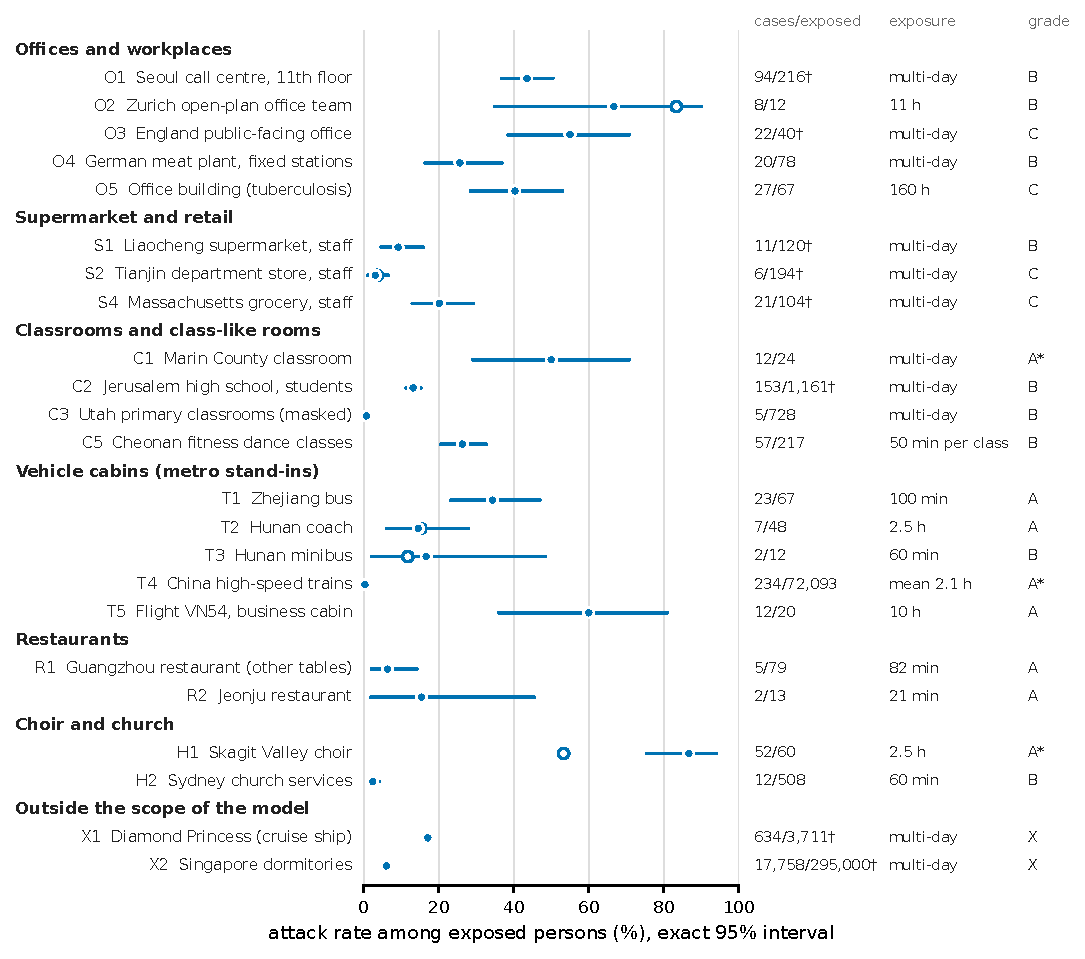
\includegraphics[width=\textwidth]{appB_dataset_attack_en}
\caption{Attack rates of the 23 records that have an exposed denominator, with exact (Clopper--Pearson)
95\,\% intervals, in the order of Table~\ref{appB_dataset:tab:records}. Filled circle: the count used in this
article; open circle: the alternative count (O2: 10 instead of 8 secondary cases; S2: 7 instead of 6;
T2: 7/46; T3: 2/17; H1: the 32 laboratory-confirmed cases only). $\dagger$: counts include the index or
primary case(s). `Multi-day' means that no duration in hours is recorded. A$*$: graded A without meeting
every grade-A criterion. The events differ in pathogen, variant, mask use, testing and number of
generations, so the attack rates are not comparable as levels of risk.}
% src: code/appB_dataset_fig_attack.py; data/appB_dataset_fig_attack.json (rows drawn)
\label{appB_dataset:fig:attack}
\end{figure}

\paragraph{Grades.}
Grade A (8 records) was defined as: a single index case, an enumerated exposed group, positions at seat or
zone level, a reported duration, and a geometry that is reported or measurable. Grade B (9 records) requires a
denominator and a duration with partial spatial information; grade C (8 records) covers aggregate,
multi-generation, abstract-only or incompletely enumerated events; the 2 out-of-scope records are graded X.
% src: data/bsc_outbreaks/outbreaks.csv (quality); data/appB_dataset_numbers.json -> grades
The re-check found that only 5 of the 8 grade-A records (T1, T2, T5, R1, R2) meet all the
grade-A criteria. The classroom C1 has no exposure duration in hours and no room size; the train cohort T4
pools 2,334 index patients and its source prints no cell denominators; and no seat or zone positions were
published for the choir H1. These three are marked A$*$. They remain in use (T4 is the only matrix of attack
rates by seat offset, H1 the benchmark for the level of the attack rate), but the dataset contains five, not
eight, single-index events with positions, a duration and a geometry.
% src: notes/VERIFICATION.md -> Section 4.4, outbreak dataset, item 1 (partially confirmed);
%      data/appB_dataset_numbers.json -> grade_A

\paragraph{Reading access.}
All 31 DOIs were confirmed in the DOI registry, and the bibliographic fields were taken from Crossref; the
re-check repeated both checks.
% src: data/bsc_outbreaks/tables/doi_verification.json; code/bsc_outbreaks/verify/results/source_check.json
The numbers were transcribed from the full text for 21 sources and from the accepted manuscript for one
\citep{miller2021}. Three sources \citep{shen2020,hu2021,hamner2020} were available only as an automated text
extraction of the publisher's web page, not as the PDF. Their numbers were compared with the abstracts and
extracted a second time in the re-check, with the same values, and two internal checks hold (the risk ratios recomputed from the zone counts of the bus,
Table~\ref{appB_dataset:tab:strata}, equal those printed by \citet{shen2020}; the train table is discussed
below). These three sources have not been checked against the PDF files. Six sources were read as abstracts
only \citep{nicholls2024,nardell1991,riley1978,moser1979,lan2021,jiang2021deptstore}; the five records that
rest on abstracts alone (O3, O5, S4, C4, T6) are graded C.
% src: data/appB_dataset_numbers.json -> sources (full 21, manuscript 1, extraction 3, abstract 6), records_resting_on_abstracts_only;
%      data/bsc_outbreaks/sources.md (Access); notes/VERIFICATION.md (Section 4.4, outbreak dataset)

\paragraph{Conflicting counts and an upper bound.}
Where sources disagree, both versions are recorded. The two investigations
of the Hunan coach give 7 cases among 48 passengers over 2.5\,h \citep{luo2020} and 7 among 46 over 200\,min
\citep{ou2022}, and they place the infected passengers differently; the minibus of the same outbreak has
2/12 against 2/17; the department store has 6 or 7 staff cases; the Zurich team has 8 or 10 first-generation
cases among 12; and 20 of the 52 choir cases are probable, not laboratory-confirmed.
% src: data/bsc_outbreaks/outbreaks.csv -> T2, T3, S2, O2, H1 (attack_rate_reported, quality_notes, n_infected_alt);
%      notes/VERIFICATION.md (Section 4.4, outbreak dataset: seat reconstructions of Luo and Ou differ)
For the Guangzhou restaurant the five secondary cases at the two neighbouring tables are an upper bound on
the number infected at the lunch. The first report of that outbreak states that at least one member of each
of the two families was infected in the restaurant and that the further cases in those families may be due
to transmission within the family \citep{lu2020}; the number infected at the lunch outside the index table
is therefore between 2 and 5. The counts marked $\ddagger$ in
Tables~\ref{appB_dataset:tab:records} and~\ref{appB_dataset:tab:strata} carry this caveat.
% src: notes/VERIFICATION.md -> Section 4.4, outbreak dataset (further points: Guangzhou counts are an upper bound);
%      notes/VERIFICATION.md (Section 4.4, outbreak dataset: Lu et al., onsets in Li et al. Table A.1)

\begin{table}[tbp]
\centering
\caption{Near/far contrasts available in the sources. Risk ratios with log-normal (Katz) 95\,\% intervals
and Fisher's exact test, computed from the counts shown. The two rows of T1 and the two rows of R1 are
alternative splits of the same people. $^{\mathrm{c}}$: one cell is zero and 0.5 was added to every cell.
$\ddagger$: upper bound (see text). $^{\mathrm{e}}$: pupils enrolled in grades 7--9 and 10--12 (581 and 583);
1,161 were tested, 580 of them in grades 10--12. For T5 the source defines the near stratum as
`$\le2$ seats away'. O1 and C2 are multi-generation outbreaks, and the position of the index
case in O1 is unknown.}
% src: data/bsc_outbreaks/outbreaks.csv -> C2 (attack_rate_reported: grades 197 + 197 + 187 = 581, 200 + 195 + 188 = 583; n_exposed 1161); data/checks/outbreak_dataset.json: jerusalem_senior_wing (583 persons, 580 tested; notes/VERIFICATION.md -> Section 4.4, outbreak dataset, further point 9); data/misc_checks.json (jerusalem; flight_label: underlined "<" before "2 seats away" in the stored copy of the source, which is not redistributed)
\label{appB_dataset:tab:strata}
\footnotesize
\setlength{\tabcolsep}{4pt}
\begin{tabular}{@{}l>{\raggedright}p{4.6cm}llll@{}}
\toprule
ID & Contrast (near against far) & Near: cases/$n$ (\%) & Far: cases/$n$ (\%) & Risk ratio (95\,\% CI) & $p$ \\
\midrule
% src: data/bsc_outbreaks/tables/near_far_risk_ratios.csv; recomputed and checked in code/appB_dataset_table.py
% >>> GENERATED strata (code/appB_dataset_table.py; do not edit by hand)
O1 & north wing against south wing (mapped seats) & 79/137 (57.7) & 4/62 (6.5) & 8.9 (3.4--23.3) & $5.2\times10^{-13}$ \\
C1 & front two rows against back three rows & 8/10 (80.0) & 4/14 (28.6) & 2.8 (1.2--6.8) & 0.036 \\
T1 & rows 5--11 (within about 2 m of the index) against rows 1--4 and 12--15 & 14/33 (42.4) & 9/34 (26.5) & 1.6 (0.8--3.2) & 0.20 \\
T1 & rows 6--10 against rows 1--5 and 11--15 (alternative split) & 11/23 (47.8) & 12/44 (27.3) & 1.8 (0.9--3.3) & 0.11 \\
T2 & rear rows 8--13 (index zone) against front rows 1--7 & 3/19 (15.8) & 4/26 (15.4) & 1.0 (0.3--4.1) & 1.0 \\
T5 & within 2 seats of the index against farther seats, business cabin & 11/12 (91.7) & 1/8 (12.5) & 7.3 (1.2--46.2) & $7.7\times10^{-4}$ \\
R1 & neighbouring tables against remote tables & 5/16$^{\ddagger}$ (31.2) & 0/63 (0.0) & 41.4$^{\mathrm{c}}$ (2.4--713) & $1.9\times10^{-4}$ \\
R1 & same air-conditioning zone against other zones (alternative split) & 5/11$^{\ddagger}$ (45.5) & 0/68 (0.0) & 63.2$^{\mathrm{c}}$ (3.7--1{,}071) & $2.0\times10^{-5}$ \\
C2 & grades 7--9 against grades 10--12 (separate wings) & 135/581 (23.2) & 18/583$^{\mathrm{e}}$ (3.1) & 7.5 (4.7--12.1) & $1.3\times10^{-26}$ \\
S1 & staff against customers & 11/120 (9.2) & 0/8{,}224 (0.0) & 1{,}563$^{\mathrm{c}}$ (92.7--26{,}381) & $3.4\times10^{-21}$ \\
% <<< GENERATED strata
\bottomrule
\end{tabular}
\end{table}

\begin{table}[tbp]
\centering
\caption{Negative controls: groups with a documented opportunity for exposure and almost no infection. The
last numerical column is the one-sided exact 95\,\% upper bound on the attack rate. The two restaurant rows
are alternative groupings of the same patrons. Access marks as in Table~\ref{appB_dataset:tab:records}.}
\label{appB_dataset:tab:controls}
\footnotesize
\begin{tabular}{@{}llllc@{}}
\toprule
Group & Record & Cases/exposed & Upper bound, \% & Source \\
\midrule
% src: data/bsc_outbreaks/tables/analysis_results.json -> negative_controls; bounds recomputed in code/appB_dataset_table.py
% >>> GENERATED controls (code/appB_dataset_table.py; do not edit by hand)
Supermarket customers & S1 & 0/8{,}224 & 0.036 & \citep{tian2021} \\
Other bus travelling to the same event & T1 & 0/60 & 4.9 & \citep{shen2020}$^{\mathrm{e}}$ \\
Restaurant, remote tables & R1 & 0/63 & 4.6 & \citep{li2021} \\
Restaurant, other air-conditioning zones & R1 & 0/68 & 4.3 & \citep{li2021} \\
Flight, premium-economy cabin & T5 & 0/35 & 8.2 & \citep{khanh2020} \\
Tested school contacts, masked classrooms & C3 & 5/728 & 1.44 & \citep{hershow2021} \\
Call-centre building, floors 7--9 & O1 & 1/595 & 0.79 & \citep{park2020} \\
% <<< GENERATED controls
\bottomrule
\end{tabular}
\end{table}

\paragraph{Spatial contrasts and negative controls.}
Table~\ref{appB_dataset:tab:strata} gives every near/far contrast that the sources allow, and
Table~\ref{appB_dataset:tab:controls} the groups used as negative controls. Three cautions apply. First, the
wing contrast of the call centre refers to the 84 case seats shown in the published plan; if the ten cases
without a seat had all worked in the south wing the ratio would be 2.6 (95\,\% interval 1.6--4.1), not 8.9.
% src: data/appB_dataset_numbers.json -> callcentre.rr, callcentre.rr_all_unmapped_south;
%      code/bsc_outbreaks/verify/results/callcentre_check.json -> wing_contrast.sens_all10_south
Second, the four single-index events with one split each (C1, T1, T2, T5) are statistically compatible with
a common risk ratio (Cochran's $Q=3.77$ on 3 degrees of freedom, $p=0.29$), so sorting events into
`near-field' and `well-mixed' ones is a reading of point estimates; the coach, with no front-to-rear
gradient, has a side-to-side contrast of 6/24 against 1/20 (risk ratio 5.0, 95\,\% interval 0.7--38).
% src: data/appB_dataset_numbers.json -> heterogeneity (cochran_Q 3.772, p 0.287), coach_side_contrast;
%      code/bsc_outbreaks/verify/results/extra_checks.json -> heterogeneity; stats_check.json -> risk_ratios (T2side)
Third, the levels are heterogeneous: over the nine SARS-CoV-2 events with a single index case and a single
exposure period, the cumulative hazard per hour, $-\ln(1-\text{attack rate})/\text{duration}$, spans a factor 34
when the 20 probable choir cases are counted and a factor 20 with confirmed cases only.
% src: data/bsc_outbreaks/tables/analysis_results.json -> hazard_per_hour_range (ratio 33.7);
%      code/bsc_outbreaks/verify/results/stats_check.json -> hazard_per_hour.confirmed_only_choir (ratio 19.97)

\paragraph{Digitisation of the call-centre floor plan.}
The seat map of record O1 was obtained from the floor plan published as Fig.~2 of \citet{park2020}; the
coordinates are derived from that figure and are not original data of this article. Desk rectangles were
segmented by colour and shape. The two open-plan wings contain 137 desks (north) and 62 desks (south). The
plan marks 84 case seats: 79 in the north wing, 4 in the south wing and 1 in the offices on the east side,
whose other desks were not digitised. The text of the source reports 94 cases among the 216 employees of
the floor, so 10 cases have no seat in the plan. The plan has no scale bar: coordinates are in units of the
desk pitch, their conversion to metres is unknown, and one employee per drawn desk is assumed.
% src: data/bsc_outbreaks/tables/park2020_callcentre_seats_digitized.csv; code/bsc_outbreaks/scripts/digitize_callcentre.py;
%      data/appB_dataset_numbers.json -> callcentre (north 79/137, south 4/62, case_seats_mapped 84, cases_unmapped 10)
The re-check typed the map again desk by desk from enlargements of the figure: the two readings match one to
one, no desk has a different case flag, and the largest difference in position is 3.8 pixels at a desk
pitch of 32.5 pixels. Figure~\ref{s8_outbreaks:fig:callcentre} is drawn from this file.
% src: code/bsc_outbreaks/verify/results/callcentre_check.json -> comparison_with_first_analysis (bijection true, 0 flags, 3.84 px);
%      data/appB_dataset_numbers.json -> callcentre.check_match, callcentre.desk_pitch_px

\paragraph{Reconstruction of the train cell counts.}
\citet{hu2021} print, for 23 seat offsets from the index passenger, an attack rate with a 95\,\% interval
but no counts. Two reconstructions were needed. On the publisher's page the five same-row values appear one
column to the left of where they belong (a contact cannot sit zero rows and zero columns away); with the
values moved to columns 1--5, the column means recomputed from the cells differ from the printed ones by
0.02 percentage points in total, against 1.17 for the layout as printed. Then, for each cell, the re-check
searched for the integer pair (cases, contacts) whose rate and Wilson interval reproduce the printed values;
we checked that every recovered pair does so to within 0.012 percentage points.
% src: data/bsc_outbreaks/tables/hu2021_train_attack_matrix.csv (realigned cells flagged);
%      code/bsc_outbreaks/verify/results/train_matrix_reconstruction.csv; verify/scripts/v02_stats.py;
%      data/appB_dataset_numbers.json -> train (column_mean_error_pp_realigned 0.024, _as_printed 1.170, max_abs_error_pp_vs_printed 0.0112)
The recovered cells sum to 230 cases among 72,692 contacts, against the 234 among 72,093 reported for the
cohort; cell denominators range from 1,033 to 5,420, and the 11 cells with at most three cases are the
least certain. The calibration of Section~\ref{M-s8_outbreaks:sec} uses these reconstructed counts. The source
itself warns that relatives and friends travelling together may have infected each other before or after the
journey, which inflates the adjacent-seat cell (3.53\,\%) most.
% src: data/appB_dataset_numbers.json -> train (230, 72692, 234, 72093, cell_n_min 1033, cell_n_max 5420, cells_with_at_most_3_cases 11);
%      code/bsc_validation/PREREGISTRATION.md, amendment V5; notes/VERIFICATION.md (Section 4.4, outbreak dataset, further point 3: Hu et al., companions)

\paragraph{Limitations and release of the first dataset.}
Investigated outbreaks are mostly large ones, so the attack rates over-represent highly infectious index
cases; records C3 and T4 are closer to ordinary exposures. Variants, mask use, vaccination and testing
differ between records and are not harmonised. Positions are zonal in most records: only T4 gives a matrix
of offsets and only O1 is resolved to seats.
% src: data/bsc_outbreaks/outbreaks.csv (quality_notes)
The released repository contains the dataset (\texttt{outbreaks.csv}, \texttt{outbreaks.json}), the list of
sources with the access level of each, the auxiliary tables (strata, risk ratios, the train matrix and its
reconstruction, the digitised seat coordinates) and the scripts that build and check them.
Copies of the source texts and figures used for transcription are not redistributed.

\subsection{The second dataset: eleven records of ten outbreaks with positions}\label{appB_dataset:sec:second}

\begin{table}[tbp]
  \centering\footnotesize
  \setlength{\tabcolsep}{2.5pt}
  \caption{The eleven records of the second dataset (Section~\ref{M-s8_outbreaks:sec:second}); W1 and W2 are the same
  ward with the same index patient. Near: within two
  rows of a source (aircraft), in the index patient's cubicle or bay (ward), within 8\,m (processing line).
  Risk ratio near/far with its 95\,\% interval. Grade A: identified source or sources, enumerated exposed
  group, positions for the whole group; B: more than one generation of cases. Role: fixed by the pathogen
  before any model was run.}
  \label{appB_dataset:tab:second}
  % generated: data/v2_tab_events2.tex (code/v2_numbers.py <- data/bsc_validation2/a1_more_outbreaks/07_descriptive.json; code/bsc_validation2/a1_more_outbreaks/PREREGISTRATION.md section 2.1)
  \begin{tabular}{@{}l>{\raggedright\arraybackslash}p{2.65cm}>{\raggedright\arraybackslash}p{1.75cm}>{\raggedright\arraybackslash}p{2.05cm}>{\raggedright\arraybackslash}p{2.2cm}>{\raggedright\arraybackslash}p{1.5cm}>{\raggedright\arraybackslash}p{1.85cm}c>{\raggedright\arraybackslash}p{1.55cm}@{}}
    \toprule
    & Event & Pathogen & Setting, duration & Position data & Near vs far & Risk ratio & Gr. & Role \\
    \midrule
    \tabinput{data/v2_tab_events2}
    \bottomrule
  \end{tabular}

  \smallskip
  \begin{minipage}{0.96\textwidth}\footnotesize
  $^{a}$\,With a continuity correction of 0.5 (a stratum without a case).
  \end{minipage}
\end{table}

\paragraph{Search and inclusion.}
The second dataset was assembled after the first test, by queries to Europe PMC for outbreaks with a seat map or
with counts by distance for the whole exposed group, and from the references of \citet{hertzberg2016risk}.
Eleven events were kept (Table~\ref{appB_dataset:tab:second}); the meat-processing line is record O4 of the
first dataset, now with its counts by distance. The events found and not used, with the reason, were fixed in
the protocol before any model was run: no identified source on board, one or two cases only, exposure before
the flight, denominators missing by seat, or positions not published (among them the aircraft outbreak of
\citet{moser1979} and the measles outbreak analysed by \citet{riley1978}). No outbreak in a
courtroom, a fitness class or a restaurant with positions for the whole exposed group was found in openly
accessible form. The search is not a systematic review, and the re-check did not repeat it.
% src: data/outbreaks2/SOURCES.md ("Events catalogued but not modelled"); code/bsc_validation2/a1_more_outbreaks/PREREGISTRATION.md section 2.2; notes/VERIFICATION.md (Section 4.6, second outbreak test, item 16: unverifiable)

\paragraph{Transcription and its checks.}
Seat maps were transcribed by eye from the published figures, and each map was checked against the totals
printed in its source before any model was run. The totals agree exactly for the flights from Hong Kong, from
Los Angeles and from Tel Aviv. They differ by one to four persons, in far strata, for three flights: 216
passengers at risk with a seat against 220 in the text for the flight from Cancun; 141 persons on the map
against 142 for the flight to Naha; 110 passengers of the mid cabin against 111 or 112 for the flight to
Perth. Two full texts are not openly accessible: the flight from Hong Kong uses the seat map as redrawn by
\citet{hertzberg2016risk}, and the tuberculosis flight only the two strata of the abstract, with seats placed
at random inside them. The counts of the ward and of the processing line were typed from the text and from an
appendix table of the sources.
% src: code/bsc_validation2/a1_more_outbreaks/POSTHOC_LOG.md (P3); data/outbreaks2/SOURCES.md
The re-check re-read every seat symbol of the four held-out flights and of the flight from Hong Kong
against the stored figures, re-typed the counts of the processing line, and fetched the abstract and
full-text numbers of the other events again; all stratum counts match. Two calibration maps (the flights from
Los Angeles and from Cancun) were not re-read seat by seat. Three limits of the data are not in the counts:
about 22 passengers of the flight to Naha who were lost to follow-up are counted as non-cases, mostly in far
rows; most non-cases of the flight from Tel Aviv were never tested; and the published figure of the ward
gives each student's bed, which the analysis replaced by random beds within the three strata (using the exact
beds changes the pooled score against the well-mixed model by $+0.13$ and nothing else). The near zone of the
flight to Naha is not the one its source analysed: the source's own group `within two rows' has 14 persons,
against the 23 in rows 21--25 used here. And one flight (AF171) was excluded as a secondary tabulation, although
two calibration events are themselves secondary in that sense (the flight from Hong Kong, from a redrawn map,
and the tuberculosis flight, from an abstract); with two cases it would change nothing.
% src: data/checks/outbreaks2.json: naha (about 22 lost to follow-up; 14 persons within two rows in the source, 23 in rows 21-25 here), ward_exact_beds (+0.13), AF171 (2 cases); notes/VERIFICATION.md (Section 4.6, second outbreak test, item 2: confirmed, with the caveats listed; further point 7; item 16: AF171 dropped as secondary tabulation, CA112 and the tuberculosis flight from a redraw and an abstract)
The released tables give, for every event, the strata, the persons at risk and the cases, and for the seat-map
events the transcribed position of every person, with the reference and the figure or table of origin.


% supp_firsttest.tex -- Supplementary Section S7: the first outbreak test in detail.
% Paths in "% src:" comments are relative to the repository root.  Units: hours and metres.
% Scripts: code/s8_outbreaks_checks.py, s8_outbreaks_numbers.py, s8_outbreaks_fig_callcentre.py,
% s8_first_test_exact.py (first test re-run with the round-off-safe propagator).
\section{The first outbreak test in detail}\label{appS_first:sec}

This section gives the details of the first outbreak test of Section~\ref{M-s8_outbreaks:sec} of the main text; its
protocol, sensitivity analyses and post-hoc log are in Section~\ref{appC_protocol:sec}.

\subsection{Structure in the first dataset}

In a cohort of contacts of 2{,}334 index cases on Chinese high-speed trains \citep{hu2021} the attack rate is
3.53\,\% in the adjacent seat and 0.03--0.25\,\% one to three rows away; the source notes that companions
travelling together inflate the adjacent-seat value.
% src: data/bsc_outbreaks/tables/hu2021_train_attack_matrix.csv; data/bsc_validation/tables.md (Table V2); notes/VERIFICATION.md (Section 4.4, outbreak dataset, further point 3)
The Seoul call centre is the only multi-generation record with seat positions
(Fig.~\ref{s8_outbreaks:fig:callcentre}). Its two wings differ: 79 of 137 desks in the north wing are case
seats against 4 of 62 in the south wing, a ratio of 8.9 (3.4--23) for the 84 mapped seats, and of 2.6
(1.6--4.1) if the ten unmapped cases all sat in the south wing.
% src: data/s8_outbreaks_checks.json (callcentre: rr, rr_if_10_unmapped_cases_in_south); code/bsc_outbreaks/verify/results/callcentre_check.json (wing_contrast)
Inside the affected wing there is no clustering at desk scale. Of the 286 pairs of adjacent desks, 91 are pairs
of cases; random relabelling of the 79 cases among the 137 desks gives $94.6\pm5.6$ ($z=-0.64$, one-sided
$p=0.76$; join-count statistic of \citet{moran1948interpretation}). In the re-check the same
seat map was obtained by reading enlarged crops of the published figure desk by desk, without the colour
segmentation, the same result for four other definitions of adjacency, and a power of at least 0.94 against
neighbour-driven spread whose local weight is at least equal to the background.
% src: data/s8_outbreaks_callcentre_figdata.json; data/bsc_outbreaks/tables/analysis_results.json (callcentre.joincount); code/bsc_outbreaks/verify/results/callcentre_check.json (joincount, power_contagion_alternative: power 0.94 at eps = 1.0)

\begin{figure}[tbp]
  \centering
  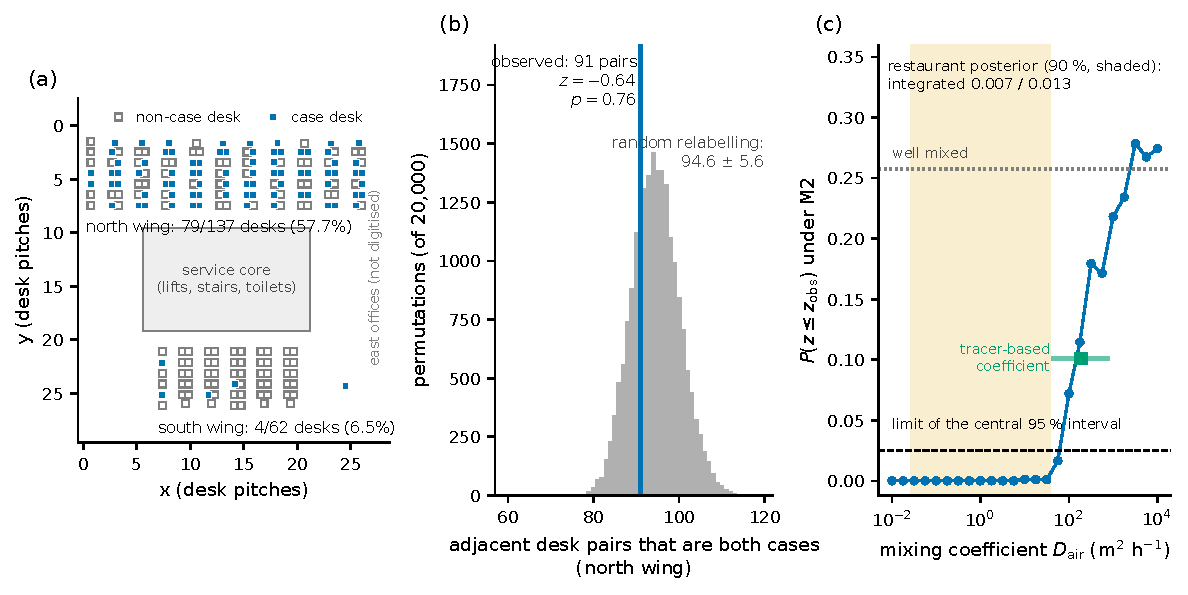
\includegraphics[width=\textwidth]{s8_outbreaks_callcentre_en}
  % generated by code/s8_outbreaks_fig_callcentre.py from data/bsc_outbreaks/tables/park2020_callcentre_seats_digitized.csv
  % and data/bsc_outbreaks/tables/callcentre_joincount_null.npy; numbers in data/s8_outbreaks_callcentre_figdata.json
  \caption{Seoul call centre, 11th floor. (a)~Desks with (filled) and without (open) a case. The positions were
  digitised by us from Fig.~2 of \citet{park2020}; the published plan has no scale bar, so coordinates are in
  desk pitches, and it shows 84 of the 94 reported case seats (one of them in the east offices, which were not
  digitised otherwise). (b)~Number of adjacent desk pairs in the north wing (centres within 1.25 desk pitches;
  286 pairs) in which both desks are case seats: observed value (line) and its distribution under 20{,}000
  random relabellings of the 79 cases among the 137 desks; $z$ is the standardised difference and $p$ the
  one-sided probability of a count at least as large as observed. (c)~Probability, under $\Mtwo$, of a
  join-count $z$ as small as observed, as a function of the mixing coefficient (25 grid values, computed in the
  re-check with a mode-sum propagator that shares the numerical defect of Section~\ref{M-s8_outbreaks:sec:holdout};
  the probability is 0 at every grid value below $5.6\sqmh$, so the defect can act only through the
  outbreak-size weights of the second integral below). Shaded: 90\,\% posterior interval of the coefficient calibrated on the
  restaurant; integrated over that posterior the probability is 0.007 (posterior draws weighted equally) or
  0.013 (weighted by their probability of producing an outbreak of the observed size), below the limit 0.025
  of the central 95\,\% interval (dashed). Dotted line: well-mixed model. Square with bar: coefficient taken
  from tracer measurements (Section~\ref{M-s8b_evidence:sec:tracer}). With the
  40 posterior draws of the Monte Carlo estimate of the protocol the probabilities were 0.017 and 0.031
  (Table~\ref{appC_protocol:tab:posthoc}, entry P5).}
  % src: data/s8_outbreaks_callcentre_figdata.json (M2_P_z_le_obs_equal_weight 0.0068, M2_P_z_le_obs_pooled_weight 0.0128, wellmixed_P_z_le_obs 0.258, tracer_P_z_le_obs 0.101); data/validation_checks/callcentre_quadrature.json
  \label{s8_outbreaks:fig:callcentre}
\end{figure}

\subsection{Calibration}\label{s8_outbreaks:sec:calibration}

Vehicle cabins are calibrated on the train cohort: binomial likelihood on 22 seat-offset
cells, with the adjacent-seat cell excluded because of the companions. Seated rooms are calibrated on the
Guangzhou restaurant \citep{lu2020,li2021}, with interval-censored counts at the two tables next to the index
table, because the first report states only that at least one member of each of those families was infected at
the lunch. The distribution of the mixing coefficient used for prediction is a pseudo-posterior: proportional to
the profile likelihood (the infectiousness parameter $\varepsilon_k$ maximised, not integrated out) times a flat
prior on $\log_{10}D$ between $10^{-2}$ and $10^{4}\sqmh$. The second test uses the same construction. For
brevity it is called the posterior below and in Section~\ref{M-s8_outbreaks:sec} of the main text.
% src: code/bsc_validation/PREREGISTRATION.md sections 2.1 (V1, V2), 3.4, 5.1

\emph{Hold-out.} Four single events (bus, coach, flight, classroom) are tested on the split of their cases
between a near and a far stratum, and the call centre on the join-count $z$ of its north wing. For each single
event $\varepsilon_k$ is set from the event total, never from the strata; the prediction is the exact
distribution of the number of near cases given the total, averaged over 300 draws of the posterior, of the
ventilation prior and of the unknown seating inside each stratum. The logarithm of its value at the observed
split is the score $S$, and $\Delta=S(\text{model})-S(\Mzero)$.
% src: code/bsc_validation/PREREGISTRATION.md sections 5.2, 6; code/bsc_validation/POSTHOC_LOG.md (300 draws instead of 400: notes/VERIFICATION.md, Section 4.5, first outbreak test item 1)

\begin{figure}[tbp]
  \centering
  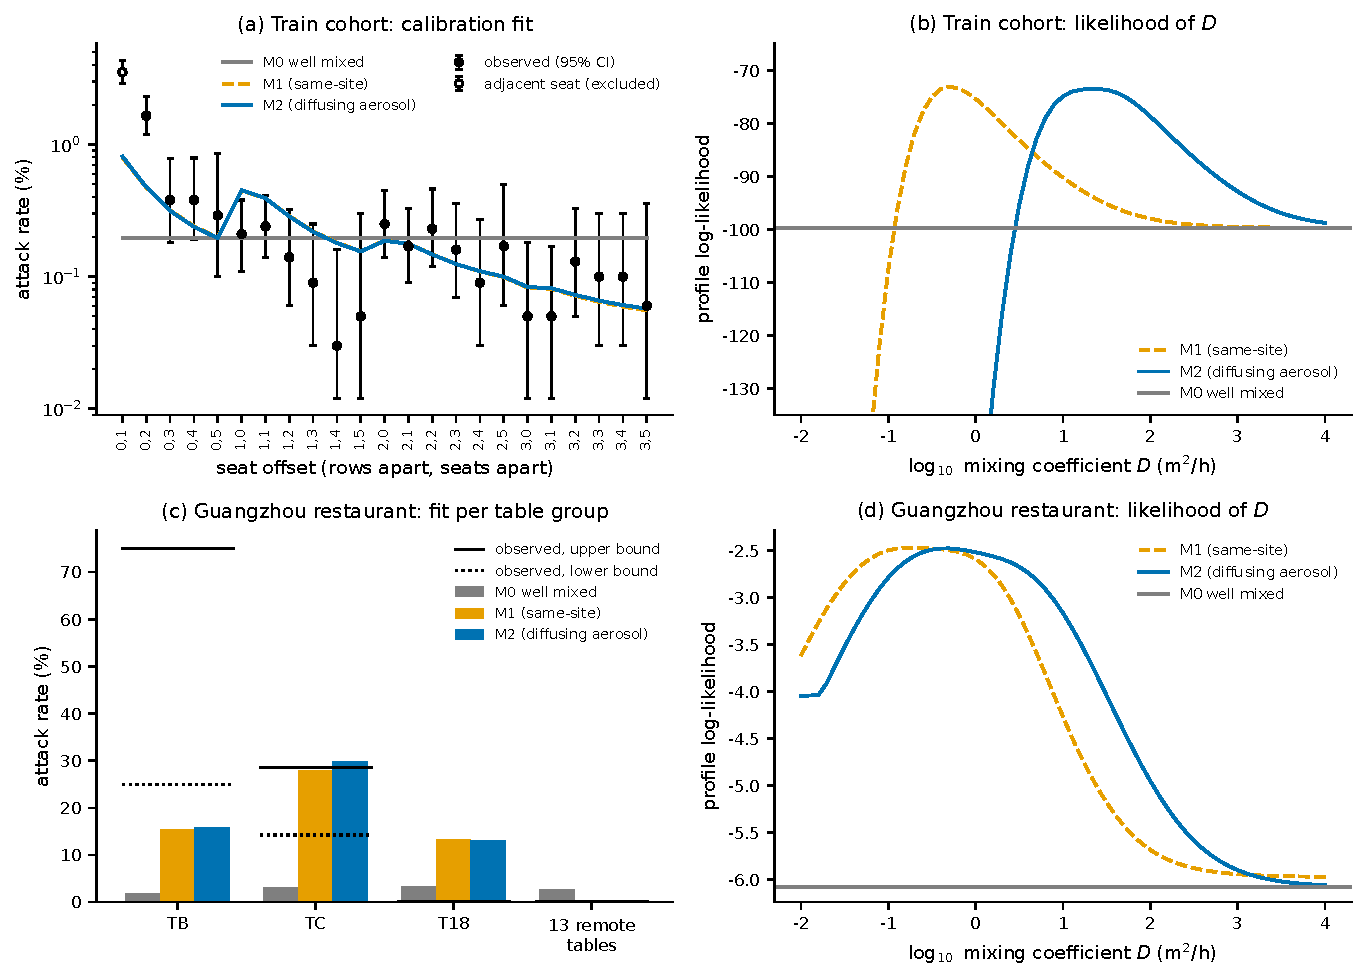
\includegraphics[width=\textwidth]{figV1_calibration_en}
  % src: figures/figV1_calibration_en.pdf (code/bsc_validation/scripts/20_figures.py <- data/bsc_validation/01_cal_T4_primary.json, data/bsc_validation/01_cal_R1_primary.json)
  \caption{Calibration of the first test. (a)~Train cohort of \citet{hu2021}: attack rate by seat offset (rows apart, seats
  apart) with 95\,\% intervals, and the fitted models; the open symbol is the adjacent seat, excluded from the
  likelihood. (b)~Profile log-likelihood of the mixing coefficient $D$ ($\Dp$ for $\Mone$, $\Dair$ for $\Mtwo$).
  (c)~Guangzhou restaurant: fitted attack rates at the two tables next to the index table (TB, TC), at the
  table across from it (T18) and at the 13 remote tables, with the bounds of the interval-censored counts; no
  case was observed at T18 or at the remote tables. (d)~As (b) for the restaurant. The models are those of
  Table~\ref{M-s8_outbreaks:tab:models}.}
  % src: data/bsc_validation/01_cal_R1_primary.json (tables: TB, TC, T05-T18 = 16 entries, 13 of class "remote"); data/bsc_outbreaks/tables/li2021_restaurant_tables.csv (T04 empty, TA = index table, excluded)
  \label{s8_outbreaks:fig:calibration}
\end{figure}

\begin{table}[tbp]
  \centering\small
  \caption{Calibration fits of the first test (in-sample). Mixing coefficient: $\Dp$ for $\Mone$, $\Dair$ for $\Mtwo$; value at
  the maximum of the likelihood and 90\,\% posterior interval. The deviance is relative to the saturated binomial model; for the restaurant the
  counts are interval-censored and no deviance is defined.}
  \label{s8_outbreaks:tab:calibration}
  % src: data/bsc_validation/tables.md (Table V1), generated from data/bsc_validation/01_cal_T4_primary.json and data/bsc_validation/01_cal_R1_primary.json; re-extracted in data/s8_outbreaks_numbers.json (calibration)
  \begin{tabular}{@{}llccc@{}}
    \toprule
    Record & Model & Mixing coefficient ($\mathrm{m^2\,h^{-1}}$) & Log-likelihood & Deviance (d.f.); $p$ \\
    \midrule
    Trains, 22 cells       & $\Mzero$ & --                  & $-99.70$ & 126.1 (21); $5\times10^{-17}$ \\
                           & $\Mone$  & 0.50 (0.31--0.79)   & $-73.12$ & 72.9 (20); $6\times10^{-8}$ \\
                           & $\Mtwo$  & 25 (9.7--43)        & $-72.97$ & 72.6 (20); $7\times10^{-8}$ \\
    Restaurant, 16 tables  & $\Mzero$ & --                  & $-6.08$  & -- \\
                           & $\Mone$  & 0.20 (0.016--14)    & $-2.47$  & -- \\
                           & $\Mtwo$  & 0.50 (0.026--39)    & $-2.48$  & -- \\
    \bottomrule
  \end{tabular}
\end{table}

On the train cohort both spatial models gain 26.6--26.7 units of log-likelihood over $\Mzero$ for one more parameter
and cannot be told apart (Table~\ref{s8_outbreaks:tab:calibration},
Fig.~\ref{s8_outbreaks:fig:calibration}a,b). $\Mtwo$ gives $\Dair=25\sqmh$ at the maximum of the likelihood
(90\,\% posterior interval 9.7--43, with its mode at $20\sqmh$ once the ventilation prior is integrated out;
8--96 if the likelihood is tempered for its over-dispersion).
% src: data/bsc_validation/tables.md (Table V1); data/s8_outbreaks_numbers.json (calibration.trains.M2: joint_max_D 25.1, mode 19.95, q05 9.67, q95 43.4); data/s8_outbreaks_v09_sens.txt ("tempered D_air 5/50/95 [8.0, 22.5, 95.6]")
Both are nevertheless rejected by the data they were calibrated on (deviance 72.6--72.9 on 20 degrees of
freedom). The isotropic kernel cannot follow the anisotropy of the train table: two seats away in the same row
the observed attack rate is 1.65\,\% and the fit 0.47\,\%; one row away in the same column they are 0.21\,\%
and 0.45\,\%.
% src: data/bsc_validation/tables.md (Table V2)
For the restaurant, with two to five cases acquired at the lunch, $D$ is identified only within three decades,
and the fitted $\Mtwo$ conflicts with the tracer-gas measurement of \citet{li2021}: the measured concentration
at the two neighbouring tables was 87--98\,\% of that at the index table and 55--86\,\% at five tables outside
their air-conditioning zone, whereas the fitted exposure is at most 0.3\,\% of the index-table value at all
seven
(Fig.~\ref{s8_outbreaks:fig:calibration}c,d). The infections were confined to one air-conditioning zone
although the air was not; an isotropic kernel can imitate this only with a coefficient that does not describe
the air.
% src: data/bsc_validation/tables.md (Tables V1, V20); data/bsc_outbreaks/tables/li2021_restaurant_tables.csv
A re-implementation with separately written code and a different propagator method reproduces the train log-likelihoods to
three decimals.
% src: notes/VERIFICATION.md (Section 4.5, first outbreak test, item 4: confirmed)

\subsection{Hold-out events}\label{s8_outbreaks:sec:holdoutdetail}

\begin{figure}[tbp]
  \centering
  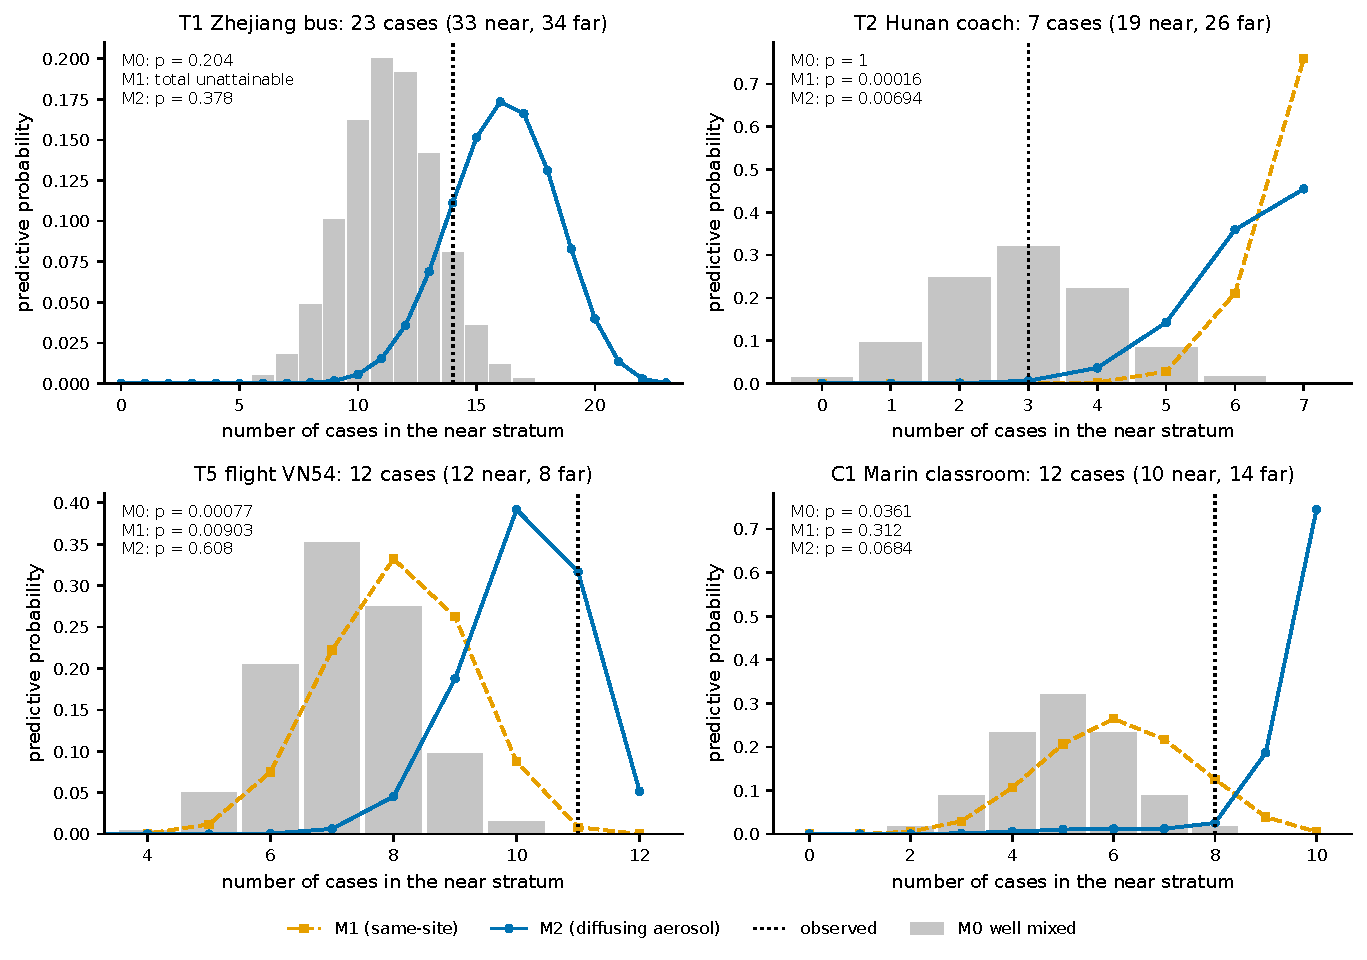
\includegraphics[width=\textwidth]{figV2_holdout_shape_en}
  % src: figures/figV2_holdout_shape_en.pdf (drawn by code/s8_first_test_exact.py with the plotting function of code/bsc_validation/scripts/20_figures.py <- data/s8_first_test_exact.json (primary), data/bsc_validation/02_predictive.json (M0), data/bsc_validation/02b_m1_exact.json)
  \caption{Hold-out events of the first test. Predictive distribution of the number of cases in the near stratum, given the total
  of the event, under $\Mzero$ (bars; hypergeometric), $\Mone$ (dashed; exact simulator for the bus, the flight
  and the classroom, closed form for the coach) and $\Mtwo$ (solid); dotted line: observed number. The
  distributions average over 300 draws of the calibrated posterior, of the ventilation prior and of the seating
  inside each stratum; $p$ is the two-sided predictive $p$-value. For the bus no $\Mone$ curve is drawn because
  the model reaches the observed total only with probability 0.0002 (Table~\ref{s8_outbreaks:tab:m1}). Exposures are computed with the
  round-off-safe propagator (see the classroom below); only the classroom curve of $\Mtwo$ differs from that
  obtained with the frozen propagator.}
  \label{s8_outbreaks:fig:holdout}
\end{figure}

Fig.~\ref{s8_outbreaks:fig:holdout} and Table~\ref{M-s8_outbreaks:tab:holdout} give the results. A
re-implementation with separately written code and its own event builders reproduced the results of the frozen code to
Monte Carlo accuracy, including, in the classroom, the numerical defect described below. We take the
events in turn for $\Mtwo$.
% src: notes/VERIFICATION.md (Section 4.5, first outbreak test, item 5)

\emph{Flight VN54: reproduced.} Eleven of the 12 passengers seated at most two seats from the index case
(`$\le2$ seats away' in the source) and one of the 8 farther away were infected. $\Mzero$ is rejected ($p=0.0008$) and $\Mtwo$ is not ($p=0.61$). The result is
robust to the calibration ($p=0.60$ at the mode of the train posterior, $20\sqmh$) and to the ventilation prior
($p=0.19$ and 1.0 when it is scaled by 1/3 and by 3). This is the one robust positive result of the first test, and it is
thin: 20 exposed passengers, among them four companion couples seated side by side, three of which are pairs
of cases. No correction for companions was applied, so the $p$-values against $\Mzero$ are too small.
% src: data/bsc_validation/03_holdout_shape.json (T5); data/validation_checks/v11_breakdown.txt (T5 at train posterior mode: p = 0.6043); data/s8_first_test_exact.json (vent."ACH x0.33".events.T5.p 0.192; vent."ACH x3.0".events.T5.p 1.0; the re-check's run, data/s8_outbreaks_v09_sens.txt, gives 0.2029 and 1.0); notes/VERIFICATION.md (Section 4.5, first outbreak test, item 3 and further point 4)

\emph{Hunan coach: failure.} Infection was uniform along the coach (3/19 rear, 4/26 front). With the
train-calibrated coefficient and the measured ventilation of the coach, $\Mtwo$ puts six of the seven cases in
the rear half (predicted ratio 11, $p=0.007$); $\Mzero$ fits exactly. The failure persists in 10 of the 12
pre-specified sensitivity variants (Table~\ref{appC_protocol:tab:sensitivity}; the pooled test passes in 11),
under the tempered posterior
($p=0.026$) and with the ventilation rate cut to a third ($p=0.040$). The model gives all 45 passengers the
same 200 minutes of exposure, whereas two of them boarded 40 minutes late and four left early.
% src: data/bsc_validation/03_holdout_shape.json (T2: p = 0.0069, k_pred_mean 6.2); data/bsc_validation/tables.md (Table V14); data/s8_outbreaks_numbers.json (sensitivity_M2: n_coach_fails 10, n_pooled_test_passes 11 of 12); data/s8_outbreaks_v09_sens.txt (tempered: T2 p 0.0262; T2 ACH x0.33: p 0.0401); notes/VERIFICATION.md (Section 4.5, first outbreak test, further point 10 and item 3: boarding and alighting not modelled)

\emph{Marin classroom: a pass that is not a prediction.} The predictive $p$-value is 0.068 (0.050 to 0.097
over five other Monte Carlo seeds), and it comes from the width of the restaurant posterior, not from the
calibrated kernel. At the posterior mode ($\Dair=0.5\sqmh$) the model infects all ten front desks and the
observed 8/10 against 4/14 is rejected ($p=0.0009$). The 63\,\% of the posterior mass between 0.1 and
$5.6\sqmh$ contributes 10\,\% of the predictive probability of the observation, and the 18\,\% below
$0.1\sqmh$ contributes 0.1\,\%; the rest, 90\,\%, comes from the diffuse upper tail above $5.6\sqmh$ (19\,\% of
the mass), where the kernel is nearly flat across the room. In 83\,\% of the posterior draws the emission rate
needed to produce the 12 cases exceeds $10^{4}\qph$ (median $8\times10^{7}$), which is not physical.
% src: data/s8_first_test_exact.json (breakdown.fixed: ranges posterior_mass 0.179, 0.630, 0.191, share_of_pmf_obs 0.0013, 0.098, 0.901; mode: D 0.501, p_two_sided 0.00093; mc: C1 p 0.0503 to 0.0974; vent.primary.events.C1: emission_q05_q50_q95 [514, 8.14e7, 8.59e17], emission_share_above_1e4 0.833)
With the frozen propagator the predictive $p$ was $0.11$, and more than half of the predictive probability came
from coefficients below $0.1\sqmh$; that half was a numerical artefact. The frozen propagator is a sum over cosine modes whose absolute error reaches about $10^{-10}$ of the largest
exposure; at coefficients of $0.1\sqmh$ and below the true exposures of the farthest desks are $10^{-33}$ to
$10^{-16}$ of that largest value, and the mode sum returns round-off noise of either sign in their place, which made far infections
look possible. The same defect was found in the second test (Section~\ref{M-s8_outbreaks:sec:second}). The values
above use a propagator that keeps the mode sum where it is resolved and replaces it elsewhere by a positive sum
of image terms; on classroom layouts this agrees with a third method (uniformisation) to better than
$10^{-8}$ relative, receiver by receiver. Only the classroom is affected: for the bus, the coach and the
flight no exposure in the posterior range is unresolved and the predictive distributions are unchanged to the
last digit; the restaurant calibration changes by about $10^{-7}$ in log-likelihood at most.
% src: data/s8_first_test_exact.json (kernel.rows: spectral_nonpositive up to 11 of 24 at D <= 0.1, spectral_min_rel down to -1.28e-10, fixed_min_rel 1.7e-33 to 6.9e-17 at D <= 0.1, fixed_vs_uniformisation_max_rel_err <= 8.4e-9; primary.pmf_change: T1, T2, T5 max_abs_change 0.0; breakdown.spectral: share 0.601 below 0.1); data/validation_checks/v11_breakdown.txt (first analysis); code/checks/outbreaks2/t6_first_set_floor.json (restaurant: bound on |dlogL| 1.1e-7)

\emph{Seoul call centre: failure.} For this multi-generation outbreak the final infection pattern was
simulated as a chain of generations with pair probabilities~\eqref{M-s8_outbreaks:eq:risk}, scaled to the
observed size. Desks are mapped to the nearest lattice site, so that the 137 desks occupy 113 distinct sites
(24 sites hold two desks, which then have the largest possible mutual exposure); the re-check found the
result unchanged on lattices two and three times finer.
% src: data/misc_checks.json (callcentre_lattice: desks 137, distinct_sites 113, sites_with_two_desks 24; code/bsc_validation/src/valmod/events.py, build_O1); data/checks/first_test.json: seoul_callcentre_M2.lattice_refinement_factors_checked (2, 3; notes/VERIFICATION.md, Section 4.5, first outbreak test, item 8)
With the restaurant-calibrated kernel $\Mtwo$ predicts strong desk-scale clustering (median
$z\approx11$), against $z=-0.64$ observed. Integrated over the posterior by quadrature, the probability of a
$z$ as small as observed is 0.007 when posterior draws are weighted equally and 0.013 when each draw is
weighted by its probability of producing an outbreak of the observed size; it depends on the arbitrary upper limit of the prior on $\log D$
(0.004 and 0.007 for $10^{3}\sqmh$; 0.013 and 0.024 for $10^{6}$) and stays below 0.025 throughout. The
observation is outside the central 95\,\% interval under either weighting
(Fig.~\ref{s8_outbreaks:fig:callcentre}c). These probabilities were computed in the re-check with its own
propagator, a mode sum that shares the numerical defect described above, and were not recomputed with the
corrected propagator. The probability of a $z$ as small as observed is 0 at every coefficient below
$5.6\sqmh$, including those at or below $0.1\sqmh$ (18\,\% of the restaurant posterior) where the defect acts,
so the equally weighted value is unaffected. The defect can act only through the outbreak-size weights of the
second value, in either direction; with zero weight at coefficients up to $0.1\sqmh$ that value would be 0.015
(0.014 with half the weight), still below 0.025, and the failure stands. The Monte Carlo estimate of the protocol, from 40 posterior draws, had given 0.017 and
0.031. $\Mzero$ is compatible ($P=0.26$). The contrast between the
wings is not counted for or against any model: the wings are separate rooms, and a lattice with a wall
reproduces any contrast if the coupling through the door is free.
% src: data/validation_checks/callcentre_quadrature.json (equal_weight 0.0068, pooled_weight 0.0128, prior_upper_limit_sensitivity; P_z_le_obs_given_D 0 at the 12 grid values up to log10 D = 0.75 (P_zero_at_all_grid_values_up_to_m2h 5.62); weight_sensitivity_at_or_below_0.1: retained_fraction_zero 0.0147, retained_fraction_halved 0.0137; posterior_mass_at_or_below_0.1 0.179); data/bsc_validation/tables.md (Table V9: M2 median z 10.99, 40-draw values 0.017 / 0.031, M0 0.262); notes/VERIFICATION.md (Section 4.5, first outbreak test, item 8: refuted)

\emph{Pooled test and what it shows.} The pooled score of $\Mtwo$ is $\Delta=+2.83$ (exact one-sided
$p=2.5\times10^{-4}$ under $\Mzero$), so A1 is passed ($+3.87$ with the frozen propagator). It rests on the flight:
without it $\Delta=-3.19$ and A1 fails; without the classroom $\Delta=+2.41$ ($p=0.0024$).
% src: data/s8_first_test_exact.json (primary.pooled.M2: all 2.835, p 2.48e-4; without_T5 -3.195; without_C1 2.406, p 0.00242); data/bsc_validation/03_holdout_shape.json (pooled.M2: 3.870, frozen propagator)

\subsection{The model with same-site transmission}\label{s8_outbreaks:sec:m1}

\begin{table}[tbp]
  \centering\small
  \caption{Reach ceiling of $\Mone$ in the exact simulator of Section~\ref{M-s6_scenes:sec} (same-site rule,
  only the index case infectious, 24 draws of $\Dp$ from the calibrated posterior). Third column: number of
  draws in which the mean number of cases can reach the observed number for some transmission rate. Fourth
  column: for the other draws, mean number of cases as the transmission rate tends to infinity (median and
  range over draws). Last column: probability that the number of cases reaches the observed number, averaged
  over the 24 draws, each at the largest transmission rate of its search (or at the rate at which its mean
  reaches the observed number).}
  \label{s8_outbreaks:tab:m1}
  % src: data/bsc_validation/tables.md (Table V8), generated from data/bsc_validation/02b_m1_exact.json
  \begin{tabular}{@{}lcccc@{}}
    \toprule
    Event & Cases / exposed & Draws reaching & Largest mean total & $\Prob(\text{total}\ge\text{observed})$ \\
    \midrule
    Zhejiang bus    & 23/67 & 0 of 24  & 8.9 (7.5--12.2) & 0.0002 \\
    Hunan coach     & 7/45  & 21 of 24 & 6.8 (6.8--6.9)  & 0.57 \\
    Flight VN54     & 12/20 & 0 of 24  & 6.3 (3.9--8.2)  & 0.025 \\
    Marin classroom & 12/24 & 2 of 24  & 1.1 (0.0--11.9) & 0.081 \\
    \bottomrule
  \end{tabular}
\end{table}

Calibrated on the trains, $\Mone$ has $\Dp=0.50\sqmh$ (0.31--0.79): a seated passenger changes site a few
times per hour; the classroom takes its mobility from the restaurant posterior, which is wide (draws from
0.02 to $15\sqmh$, median 0.2). At these mobilities the mean number of cases stays below the observed number in
three of the four held-out events, however large the transmission rate, because the attack rate saturates at the probability
that a susceptible ever shares a site with the index case (Table~\ref{s8_outbreaks:tab:m1}). The mean number
of cases is at most about 9 on the bus, where 23 were observed, about 6 in the business cabin (12 observed) and
about 1 in the classroom at the posterior mode (12 observed). The observed total itself is reached with
probability 0.0002 on the bus, 0.025 on the flight and 0.081 in the classroom (averaged over the posterior draws;
on the flight the largest simulated total is 19, in the classroom six draws give the observed total a positive
probability, three of them 0.55 to 0.61). Under the rule adopted when this was found (post-hoc log, item P4:
a total reached with probability below 0.01 counts as a failure), only the bus total is unattainable. A
separately written simulator gives 9.1 for the bus, with no replicate reaching 23.
% src: data/bsc_validation/02b_m1_exact.json (events.*.rows: p_total_ge_K, mean 0.00019 (T1), 0.0247 (T5, 0.0016-0.094 in all 24 draws, max_total 19), 0.0810 (C1, non-zero in 6 draws, largest 0.549, 0.590, 0.605)); data/bsc_validation/tables.md (Table V8); code/bsc_validation/POSTHOC_LOG.md (P4); notes/VERIFICATION.md (Section 4.5, first outbreak test, item 7: confirmed)
Where the total can be reached, the pattern is wrong: on the coach $\Mone$ predicts a ratio of 34
($p=0.0002$), and on the flight a pattern that is too flat ($p=0.009$). Its pooled score is $-2.94$
(Table~\ref{M-s8_outbreaks:tab:holdout}).
% src: data/bsc_validation/03_holdout_shape.json (T2.M1, T5.M1, pooled.M1)

\subsection{Mixing coefficients and levels}

\begin{figure}[tbp]
  \centering
  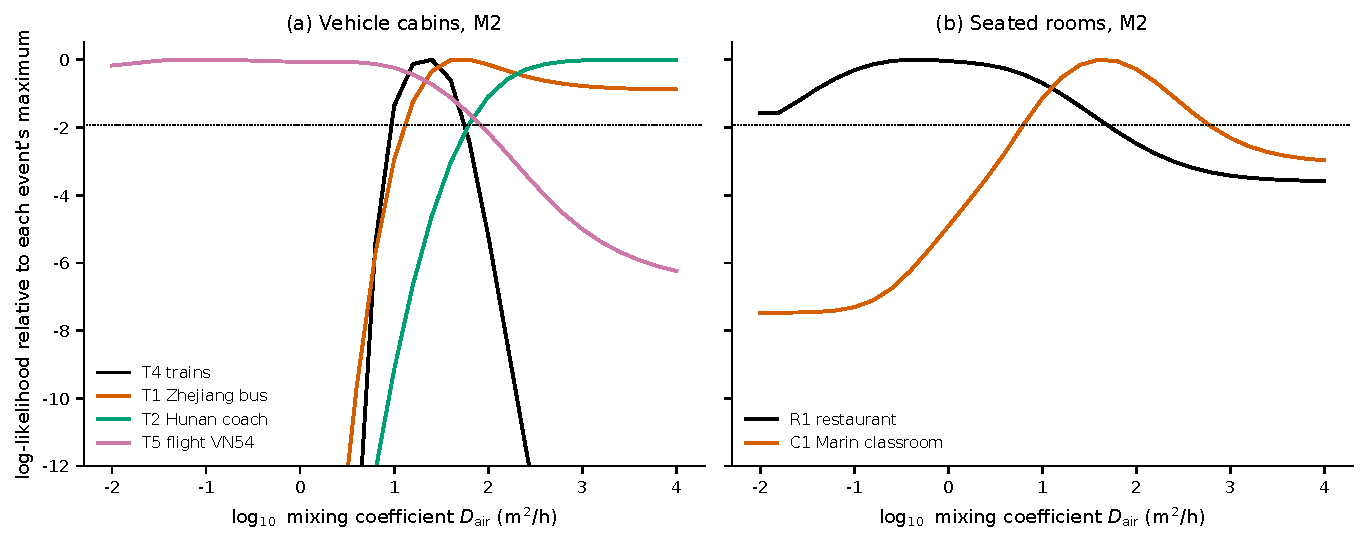
\includegraphics[width=0.95\textwidth]{figV8_mixing_heterogeneity_en}
  % src: figures/figV8_mixing_heterogeneity_en.pdf (drawn by code/s8_first_test_exact.py <- data/s8_first_test_exact.json (loo_room) and data/bsc_validation/07_loo.json (vehicles))
  \caption{Log-likelihood of the mixing coefficient $\Dair$ of $\Mtwo$ for each event taken alone, relative to
  its maximum: (a)~vehicle cabins, (b)~seated rooms. The horizontal line at $-1.92$ bounds the 95\,\% likelihood
  interval of each event. For the hold-out events the likelihood is that of the near/far split given the
  total.}
  \label{s8_outbreaks:fig:mixing}
\end{figure}

Fitted alone, the vehicle events of the first test ask for mixing coefficients that differ by orders of magnitude
(Fig.~\ref{s8_outbreaks:fig:mixing}): 0.06--$0.1\sqmh$ for the flight, 25 for the trains, 63 for the bus, and
at least $6{,}300\sqmh$ for the coach, whose likelihood is flat up to the end of the grid ($10^4\sqmh$). A
common value is rejected: the likelihood ratio is 9.52 on 3 degrees of freedom (9.56 in the re-check), with
its maximum at $40\sqmh$, and $p=0.023$ from the chi-square reference. That $p$ is approximate: the coach's
maximum lies on the edge of the grid and each event has few cases, so the regularity conditions of the
reference distribution are not met. This analysis was added after the
primary results were seen. The protocol expected the measured ventilation rate to explain which cabins show a
gradient; it does not explain the coach. The coefficient calibrated in one setting therefore cannot be assumed
to transfer to another.
% src: data/appC_protocol_numbers.json (loo.vehicle: LR 9.52, p 0.0231); data/bsc_validation/07_loo.json (classes.vehicle.M2: D_own_mode 25.1, 63.1, 6310, 0.1; joint_D_mode 39.8); data/validation_checks/v10_c1_loo.txt (T1 63.1, T2 6309.6, T5 0.063, T4 25.1; LR 9.56, p = 0.0227, common-D maximum at 39.8); data/bsc_validation/tables.md (Tables V16, V17: flight 0.1); code/bsc_validation/POSTHOC_LOG.md (P10)

\begin{table}[tbp]
  \centering\small
  \caption{Emission rate implied by each event, in quanta per hour at a breathing rate of
  $0.5\,\mathrm{m^3\,h^{-1}}$. Upper block: well-mixed scaling (shared by $\Mzero$ and $\Mtwo$ for a group spread
  over the room), with the exact binomial 95\,\% interval. Lower block: emission that $\Mtwo$ needs in the
  hold-out events (median and 5--95\,\% range over the calibrated posterior and the ventilation prior; for the
  classroom with the round-off-safe propagator).
$\remrate$: prior median (upper block).}
  \label{s8_outbreaks:tab:levels}
  % src: data/bsc_validation/tables.md (Table V10), from data/bsc_validation/04_level_controls.json (implied.*, E_T4); lower block: data/s8_outbreaks_v09_sens.txt ("implied emission quanta/h under M2, 5/50/95%"; bus, coach, flight); classroom: data/s8_first_test_exact.json (vent.primary.events.C1.emission_q05_q50_q95: 514, 8.14e7, 8.59e17)
  \setlength{\tabcolsep}{3.8pt}
  \begin{tabular}{@{}lcccc@{}}
    \toprule
    Event & Cases / exposed & Duration (h) & $\remrate$ ($\mathrm{h^{-1}}$) & Implied emission \\
    \midrule
    Skagit Valley choir \citep{hamner2020}  & 52/60$^{a}$ & 2.5  & 1.6  & 2{,}734 (1{,}904--3{,}832) \\
    Jeonju restaurant \citep{kwon2020}      & 2/13        & 0.35 & 1.2  & 1{,}921 (223--6{,}969) \\
    Zurich office \citep{weissberg2020}     & 8/12        & 11   & 1.9  & 768 (300--1{,}614) \\
    Cheonan fitness classes \citep{jang2020}& 57/217$^{d}$ & 1.7 & 2.5  & 283 (214--367) \\
    Hunan minibus \citep{ou2022}            & 2/17$^{e}$  & 1.0  & 10.5 & 63 (7--229) \\
    Hunan coach \citep{ou2022}              & 7/46$^{e}$  & 3.3  & 5.7  & 36 (14--74) \\
    Trains (mean per index case)            & 230/72{,}692 & 2.1 & 6--21 & 1.3 (0.8--2.3)$^{b}$ \\
    \midrule
    Zhejiang bus ($\Mtwo$)                    & 23/67       & 1.7  &      & 132 (103--231) \\
    Hunan coach ($\Mtwo$)                     & 7/45$^{e}$  & 3.3  &      & 46 (34--67) \\
    Flight VN54 ($\Mtwo$)                     & 12/20       & 10   &      & 1{,}594 (435--11{,}823) \\
    Marin classroom ($\Mtwo$)                 & 12/24       & 13$^{c}$ &  & $8\times10^{7}$ ($514$--$9\times10^{17}$) \\
    \bottomrule
  \end{tabular}

  \smallskip
  \begin{minipage}{0.96\textwidth}\footnotesize
  $^{a}$\,Includes 20 probable cases; 1{,}034 quanta per hour with the 32 confirmed cases only. At a breathing
  rate of $1.0\,\mathrm{m^3\,h^{-1}}$, the middle of the range 0.65--1.38 sampled by \citet{miller2021}, the
  value is about 1{,}370 quanta per hour; they report $970\pm390$ for the same event, with lower loss rates.
  $^{b}$\,90\pct{} posterior interval.
  $^{c}$\,Assumed (two school days of 6.5 hours); the source does not report hours.
  $^{d}$\,Not a single-index event: eight infected instructors taught classes in 12 facilities; 57 is derived
  from the reported attack rate (26.3\pct{} of 217), and the emission is computed as if for one index case in
  one room of $180\,\mathrm{m^3}$.
  $^{e}$\,Counts of \citet{ou2022}: 46 persons on the coach including the driver in their dose table, 45
  passengers with a seat in their stratum table (\citet{luo2020} report 7/48); 17 persons in the minibus
  (\citet{luo2020}: 2/12).
  \end{minipage}
  % src: data/bsc_validation/04_level_controls.json (implied.H1.E_implied = 2734.3, E_implied_alt = 1034.3); data/refs_search.json (manual_checks.miller2021: breathing rate uniform on 0.65-1.38 m3/h, loss rates, 970 +- 390); data/misc_checks.json (miller: 2734.3 x 0.5 / 1.0 = 1367); data/bsc_outbreaks/outbreaks.csv rows C5 (exposure_type, derived_fields), T2, T3 (attack_rate_reported); code/bsc_validation/POSTHOC_LOG.md (P9)
\end{table}

One infectiousness parameter is fitted per event, in both tests, so no attack rate in this section is a
prediction. The second test conditions on the event totals and has no level check; the following numbers are
those of the first. The
implied emission rates span a factor of 76 across five single-index events and one cluster with several
instructors, from 36 quanta per hour on the coach to 2{,}734 at the choir rehearsal (a factor of 53 if only the confirmed choir cases are counted), and
the train cohort, which is not selected for large outbreaks, has a mean of 1.3 (0.8--2.3)
(Table~\ref{s8_outbreaks:tab:levels}). Published outbreaks are selected for being large; their level cannot be
predicted from a typical index case.
% src: data/bsc_validation/04_level_controls.json (implied.H1.E_implied = 2734.3, E_implied_alt = 1034.3; implied.T2.E_implied = 36.0; implied.R2.E_implied = 1921.0; E_T4.q); ratios 2734.3/36.0 = 76, 1921.0/36.0 = 53
For the one event that $\Mtwo$ reproduces, the flight, the emission it needs is about 1{,}600 quanta per hour
(435--11{,}800); for the classroom the median is $8\times10^{7}$.
% src: data/s8_outbreaks_v09_sens.txt (T5 [435.4, 1593.6, 11823.4]); data/s8_first_test_exact.json (vent.primary.events.C1.emission_q05_q50_q95: median 8.14e7)
Two level checks have a defined reference. The same index case rode the Hunan coach and then a minibus:
fitted on the coach, $\Mtwo$ predicts 1.3 cases among the 17 people in the minibus (90\,\% interval 0--4); 2
were observed. Anchored on the train mean, $\Mtwo$ predicts 2.1 cases (0--5) among 728 contacts in masked Utah
classrooms \citep{hershow2021} with an assumed mask factor of 0.35; 5 were observed. Both checks pass, and
neither is sharp: the second fails at a mask factor of 0.2 (predicted 1.2, interval 0--3), inside the
pre-specified range 0.2--0.6. No negative control fails (Table~\ref{appB_dataset:tab:controls}), but the
criterion has almost no power: the premium-economy cabin of the flight (0 of 35 infected) passes although the
95th percentile of the predicted attack rate, 18.6\,\%, is more than twice the one-sided 95\,\% upper bound
of the observation, 8.2\,\%.
% src: data/bsc_validation/tables.md (Tables V12, V13); data/bsc_validation/04_level_controls.json (tied_T2_T3.M2, C3, T5_PE); data/validation_checks/v13_c3.txt; notes/VERIFICATION.md (Section 4.5, first outbreak test, item 10)

\subsection{Outcome of the first test}\label{s8_outbreaks:sec:outcomedetail}

\begin{table}[tbp]
  \centering\small
  \caption{First test: decision rule applied to both models, with the corrections of the re-check and the
  numerical correction of the classroom (Section~\ref{M-s8_outbreaks:sec:holdout}). The
  call-centre probabilities are given for the two weightings of posterior draws (by outbreak probability;
  equal); those for $\Mone$ are from the 40 posterior draws of the protocol and were not recomputed by
  quadrature. Outcome W4: two or more adequacy failures; no general statement of agreement is
  licensed.}
  \label{s8_outbreaks:tab:verdict}
  % src: data/bsc_validation/tables.md (Table V18); data/bsc_validation/10_decision.json; data/s8_first_test_exact.json (primary.pooled.M2: 2.835, 2.48e-4, without_T5 -3.195; failed [T2]); notes/VERIFICATION.md (Section 4.5, first outbreak test, item 11); data/validation_checks/*
  \begin{tabular}{@{}>{\raggedright\arraybackslash}p{0.25\textwidth}>{\raggedright\arraybackslash}p{0.32\textwidth}>{\raggedright\arraybackslash}p{0.37\textwidth}@{}}
    \toprule
    Criterion & $\Mone$ (same-site) & $\Mtwo$ (diffusing aerosol) \\
    \midrule
    A1 pooled test against $\Mzero$ & $\Delta=-2.94$: fail &
        $\Delta=+2.83$, $p=2.5\times10^{-4}$: pass ($-3.19$ without the flight) \\
    A2 single events & fail: bus (total unattainable), coach, flight & fail: coach \\
    A2 call-centre join count & inside ($P=0.056$; 0.040) & outside ($P=0.013$; 0.007) \\
    A3 level checks & minibus inside; classrooms outside &
        minibus inside; classrooms inside at mask factor 0.35, outside at 0.2 \\
    A4 negative controls & none fails & none fails (criterion nearly powerless) \\
    \midrule
    Outcome & W4 & W4 \\
    \bottomrule
  \end{tabular}
\end{table}

Table~\ref{s8_outbreaks:tab:verdict} applies the rule of the first test. The outcome is W4 for both models:
$\Mone$ fails the pooled test and three single events; $\Mtwo$ passes the pooled test and fails two adequacy
tests, the coach and the call centre. In the re-check the calibration, the hold-out predictions and the
call-centre test were re-implemented and the counts retyped from the sources; the call-centre probabilities by
quadrature and the comparison with a constant ratio come from it. Its propagator shared the numerical defect of the
classroom, whose correction changes no verdict. The second test has the outcome V5 for $\Mtwo$ and for $\Mone$
(Section~\ref{M-s8_outbreaks:sec:second} of the main text); in its re-check every number that decides the outcome was
reproduced, the held-out seat maps were re-read against the published figures, and the comparisons that qualify it
were added. Fig.~\ref{s8_outbreaks:fig:summary} shows all events together.
% src: notes/VERIFICATION.md (Section 4.5, first outbreak test, summary); notes/VERIFICATION.md (Section 4.6, second outbreak test, summary: the re-implementation reproduces every headline number and the registered outcome V5)

\paragraph{What these data cannot decide.} (i)~Whether the same-row excess in the train table is air or
companions. The choice decides two verdicts of the first test: with the adjacent-seat cell included in the
calibration the bus is rejected as well and the pooled score is $-4.9$; with the whole index row excluded
nothing fails and it is $+4.9$.
% src: data/s8_first_test_exact.json (sens.S-adj.M2: delta -4.857, failed [T1, T2]; sens.S-row.M2: delta +4.905, failed [])
(ii)~The kernel in rooms: the restaurant has two to five informative cases, and the two ward datasets of the
second dataset contradict each other. (iii)~Anything about level. (iv)~The definition of near: on aircraft the
comparison with the constant ratio changes sign with the near zone and the strata
(Section~\ref{M-s8_outbreaks:sec:second}), and the two-row zone is itself a rule derived from earlier outbreaks,
one of them a calibration event here. (v)~The models ignore documented features of the events: the bus
passengers attended a 150-minute event together, coach passengers boarded and left at different stops,
households sat together on the flights, and most passengers of one flight were never tested. Seat maps were
transcribed by eye from published figures; those of the held-out events were re-read in the re-check
and found to match, two calibration maps were not re-read seat by seat.
% src: notes/VERIFICATION.md (Section 4.5, first outbreak test, further point 10); notes/VERIFICATION.md (Section 4.6, second outbreak test, items 2, 5, further points 3 and 7)

% supp_protocol1.tex -- Supplementary Section S8: protocol of the first outbreak test, sensitivity analyses and post-hoc log.
% Paths in "% src:" comments are relative to the repository root.
% Every table row marked "generated" is pasted from data/appC_protocol_tables.tex, written by
% code/appC_protocol_tables.py; every other number of this appendix is stored, with its source key,
% in data/appC_protocol_numbers.json (same script).
\section{Protocol of the first outbreak test, sensitivity analyses and post-hoc log}\label{appC_protocol:sec}

This section documents the first test of Section~\ref{M-s8_outbreaks:sec} of the main text (the second test and the
further analyses are documented in Section~\ref{appS_prot2:sec}): what was fixed before any model was run,
the decision rule and its power, the sensitivity analyses, and every choice made after results had been seen.
The protocol, its power addendum, the freeze record and the post-hoc log are released with the code as
redacted copies: passages that do not concern the analyses of this article are omitted or reworded, and
identifiers are renamed as in the rest of the repository; the repository lists every changed line
(\texttt{code/REDACTIONS.md}). The SHA-256 hashes of the freeze records refer to the unredacted originals, which
are kept by the author and can be provided to the editor and referees; the timing evidence, self-attested in any
case, can therefore not be checked from the repository alone.
The protocol file is named \texttt{PREREGISTRATION.md} and describes itself as a pre-registration; it was not
lodged with any registry, and in this article it is called the protocol and its contents pre-specified.
`The re-check' denotes the second pass of Section~\ref{M-s1_intro:sec}: a re-implementation of the whole
analysis with separately written code, within the same project and on the same machine; where it corrected a
result, the corrected result is the one reported. Where the frozen protocol texts speak of a
`verifier', they mean this same-project re-check, not an independent party, and
by `the analyst' they mean the first analysis (both passes were made by the author).
% src: code/bsc_validation/README.md (PREREGISTRATION.md, PREREG_ADDENDUM_A1_power.md, PREREG_FREEZE.json, POSTHOC_LOG.md); notes/VERIFICATION.md (Section 4.5, first outbreak test, summary)

\subsection{What was frozen, and the evidence for when}\label{appC_protocol:sec:freeze}

The protocol was frozen on 1~October 2026 at 05:12:03 (British Summer Time, as are all times below). The
freeze record holds the SHA-256 hashes of six files: the protocol text (hash beginning \texttt{632db9b7}), the
modules that define the event geometries, the lattice kernels, the statistics and the interface to the exact
simulator, and the file of hold-out stratum counts. Recomputed for this article on the unredacted originals,
all six hashes match.
% src: code/bsc_validation/PREREG_FREEZE.json (frozen_at, sha256); data/appC_protocol_numbers.json -> freeze.hash_basis ("hashes recomputed on the unredacted original files in the author's working tree"), freeze.hashes.*.sha256_recomputed_on_original, freeze.all_hashes_match (true, 6 files); a run in the public repository checks the redacted copies against code/REDACTIONS.json instead
These files fix the observation model of every event (Table~\ref{appC_protocol:tab:obs}), the three models
(Table~\ref{M-s8_outbreaks:tab:models}), the split into calibration and hold-out records, the estimation
procedure, the metrics, the decision rule (Table~\ref{appC_protocol:tab:rule}) and twelve sensitivity
analyses. Table~\ref{appC_protocol:tab:amend} lists how they depart from the protocol first proposed with the
dataset, which is released as a redacted copy (\texttt{code/bsc\_outbreaks/PROTOCOL\_PROPOSAL.md}).
% src: code/bsc_validation/PREREGISTRATION.md sections 2, 4, 5, 6, 8, 9

The protocol text was last modified at 05:04:36. The first calibration run started at 05:13:30. The predictive
distributions of the hold-out events and the power of the rule were stored at 05:15:43 and 05:15:46, by a
script that does not read the hold-out counts, and the first comparison with those counts was stored at
05:19:04. The intervals are minutes because the protocol, the code and the runs were prepared in one
continuous stretch of work; the re-check (Section~\ref{M-s1_intro:sec}) was a separate, later pass.
% src: data/appC_protocol_numbers.json -> freeze.file_times_local (PREREGISTRATION.md modified 05:04:36; PREREG_FREEZE.json created 05:12:03, modified 05:29:32; data/bsc_validation/02_predictive.json 05:15:43; data/bsc_validation/02_power.json 05:15:46; data/bsc_validation/03_holdout_shape.json 05:19:04; code/bsc_validation/src/valmod/predict.py modified 05:21:59), freeze.first_calibration_log_line ("2026-10-01 05:13:30 BST start T4:primary")

Four limits apply. (i)~The protocol is \emph{data-aware} and only \emph{model-blind}: the outbreak
counts had been read before the protocol was written, and the strata, the ventilation priors and the exclusion
of the adjacent-seat cell were chosen with that knowledge. (ii)~The evidence for the order of events is
file-system metadata alone. There is no version-control history, and the freeze record was itself rewritten at
05:29:32, when the hashes were re-checked, so its time of freezing is self-reported. (iii)~The code that
computes the hold-out predictions and applies the rule was written after the calibration results had been seen
and is not among the hashed files; one module was edited at 05:21:59, after the hold-out counts had been read.
The re-check re-ran the current code and recovered the stored predictive distributions exactly.
(iv)~Two details differ from the protocol text: the $p$-value of A1 is computed by exact enumeration, not from
20{,}000 Monte Carlo replicates, and the predictive distributions average 300 draws where the text says 400.
% src: notes/VERIFICATION.md (Section 4.5, first outbreak test, items 1 and 13: partially confirmed); code/bsc_validation/PREREGISTRATION.md section 0

\begin{table}[tbp]
  \centering\footnotesize
  \caption{Changes to the protocol first proposed with the dataset, all made before any model was run. V1--V7
  were required by the re-check of the dataset (Section~\ref{appB_dataset:sec}); D1--D6 were forced by
  gaps in the data. The analyses S-\dots{} are those of Table~\ref{appC_protocol:tab:sensitivity}.}
  \label{appC_protocol:tab:amend}
  % src: code/bsc_validation/PREREGISTRATION.md sections 2.1, 2.2 (wording shortened); notes/VERIFICATION.md (Section 4.4, outbreak dataset)
  \begin{tabular}{@{}l>{\raggedright\arraybackslash}p{0.43\textwidth}>{\raggedright\arraybackslash}p{0.47\textwidth}@{}}
    \toprule
    & Objection or gap & Amendment or consequence \\
    \midrule
    V1 & Restaurant counts are an upper bound: the first report states only that at least one member of each
         of two neighbouring families was infected at the lunch \citep{lu2020} &
         interval-censored likelihood (1--3 of 4 at one table, 1--2 of 7 at the other); the index case's own
         table is excluded; S-R1-upper, S-R1-lower \\
    V2 & Train cohort: companions inflate the risk, most of all in the adjacent seat \citep{hu2021} &
         adjacent-seat cell excluded from the likelihood; no near-field factor transferred to hold-out
         events; S-adj, S-row, S-nu \\
    V3 & Three `grade A' records do not meet the grade criteria (classroom: no hours, no room size; trains:
         pooled index cases, no denominators; choir: no positions) &
         classroom size, hours and ventilation enter as explicit priors, and its test conditions on the class
         total; trains used as a pooled cohort; choir used for level only \\
    V4 & The pattern criterion first proposed ($|z|<1.96$ on the log risk ratio) is passed by any constant near/far
         ratio between 1.16 and 3.19, and the level criterion by a constant hazard &
         rule replaced by A1--A4 (Table~\ref{appC_protocol:tab:rule}); power computed before unblinding
         (Table~\ref{appC_protocol:tab:power}) \\
    V5 & The train table prints percentages and intervals but no cell denominators &
         cell counts reconstructed (230/72{,}692 against the reported 234/72{,}093), binomial likelihood;
         S-logit \\
    V6 & `Three regimes' of proximity gradient are not established (heterogeneity $p=0.29$) &
         no analysis assumes them \\
    V7 & The contrast between the wings of the call centre depends on ten unmapped cases &
         not used as a test; the join count inside the north wing is used \\
    \addlinespace
    D1 & Seat maps of the bus, the coach, the minibus, the aircraft cabin, the classroom and the restaurant
         were not digitised &
         published stratum sizes and index seat are used; the unknown occupied seats inside each stratum are
         drawn at random and averaged over (300 configurations) \\
    D2 & Meat-processing plant \citep{guenther2020}: appendix counts not transcribed & not evaluated \\
    D3 & Jerusalem school \citep{steinzamir2020}: needs coupled rooms; no per-class denominators & not
         evaluated \\
    D4 & Sydney church \citep{katelaris2021}: no room dimensions & excluded from the level checks \\
    D5 & A square lattice cannot place one seat per site in 3+2 seating &
         rectangular lattice with one site per seat position and hop rates $D/a_x^2$, $D/a_y^2$ \\
    D6 & Index seat on the flight not in the stored text of the source &
         uniform over the 28 business-class seats; S-5K \\
    \bottomrule
  \end{tabular}
\end{table}

\begin{table}[tbp]
  \centering\footnotesize
  \caption{Observation model of each event, as frozen. Lattices have reflecting walls and one site per seat
  position; pitches are across $\times$ along the cabin. Strata are those of the sources, with their sizes in
  brackets. The row pitches of the trains and the flight, the width of the bus, the classroom plan and hours,
  and three ceiling heights are assumptions of the protocol, not data.}
  \label{appC_protocol:tab:obs}
  % src: code/bsc_validation/PREREGISTRATION.md section 4; code/bsc_validation/PREREG_ADDENDUM_A1_power.md section A1.5 (controls); data/misc_checks.json (callcentre_lattice: 137 desks on 113 sites; code/bsc_validation/src/valmod/events.py, build_O1)
  \begin{tabular}{@{}>{\raggedright\arraybackslash}p{0.18\textwidth}>{\raggedright\arraybackslash}p{0.24\textwidth}>{\raggedright\arraybackslash}p{0.13\textwidth}>{\raggedright\arraybackslash}p{0.24\textwidth}>{\raggedright\arraybackslash}p{0.09\textwidth}@{}}
    \toprule
    Event and role & Lattice & Index case & Statistic & Duration \\
    \midrule
    Trains \citep{hu2021}; calibration, vehicles &
      $17\times6$ sites (3 seats, aisle, 2 seats); $0.5\times1.0$\,m &
      every seat in turn &
      attack rate in 23 seat-offset cells, model averaged over all seat pairs; 22 cells in the likelihood &
      gamma, mean 2.1\,h, SD 1.8\,h \\
    Restaurant \citep{lu2020,li2021}; calibration, rooms &
      $17\times8$ sites, 1\,m; height 3.14\,m; 18 tables on a $6\times3$ grid &
      index table &
      censored counts at the two neighbouring tables, zero at the others; remote layout averaged over &
      23--82\,min, per table \\
    \addlinespace
    Bus \citep{shen2020}; hold-out &
      $15\times6$ sites (3 seats, aisle, 2 seats); $0.42\times0.75$\,m; height 2.0\,m &
      row 8, middle of the 3-seat side &
      rows 5--11 (33) against other rows (34) &
      $2\times50$\,min \\
    Coach \citep{ou2022}; hold-out &
      $13\times5$ sites; $0.5\times0.877$\,m; $60.42\,\mathrm{m^3}$ &
      seat 12D &
      rear rows 8--13 (19) against front rows 1--7 (26) &
      200\,min \\
    Flight \citep{khanh2020}; hold-out &
      business cabin $7\times6$ sites, $0.9\times1.1$\,m, inside a 46-row cabin &
      uniform over 28 seats &
      the 12 occupied seats nearest the index against the other 8 &
      10\,h \\
    Classroom \citep{lamhine2021}; hold-out &
      $11\times13$ sites, 1\,m; 25 desks at 2-site pitch &
      teacher, front centre &
      front two rows (10) against back three (14) &
      13\,h \\
    Call centre \citep{park2020}; hold-out &
      137 digitised desks of the north wing, each mapped to the nearest lattice site (113 distinct sites);
      desk pitch uniform on 1.0--1.6\,m &
      uniform over desks &
      join-count $z$ of the final pattern of a chain of generations scaled to a mean of 79 cases; outbreaks
      of 69--89 cases kept &
      steady state \\
    \addlinespace
    Minibus \citep{ou2022}; level, same index as the coach &
      $6\times4$ sites; $21.69\,\mathrm{m^3}$ & row 4 & cases among 17 exposed & 60\,min \\
    Choir, office, restaurant, fitness classes \citep{hamner2020,weissberg2020,kwon2020,jang2020}; level &
      volume only: 810; 1{,}890; 309; $180\,\mathrm{m^3}$ & -- (fitness classes: eight instructors, treated as
      one index) &
      implied emission from 52/60, 8/12, 2/13, 57/217 (57 derived from 26.3\pct) &
      2.5\,h; 11\,h; 21\,min; 100\,min \\
    Utah classrooms \citep{hershow2021}; level and control &
      volume log-uniform on 180--$350\,\mathrm{m^3}$ & 51 index cases &
      cases among 728 contacts, emission anchored on the train mean & 6.5--13\,h \\
    Supermarket customers \citep{tian2021}; premium economy of the flight; one metro ride
      \citep{furuse2020}; controls &
      $6{,}000\,\mathrm{m^3}$; 30 sites of the cabin lattice; $148.5\,\mathrm{m^3}$ & -- &
      predicted attack rate against the 95\,\% upper bound of 0/8{,}224 and of 0/35; probability of five or
      more cases among 309 riders &
      27\,min; 10\,h; 20\,min \\
    \bottomrule
  \end{tabular}
\end{table}

\subsection{Decision rule and its power}\label{appC_protocol:sec:rule}

\begin{table}[tbp]
  \centering\footnotesize
  \caption{Decision rule, evaluated separately for $\Mone$ and $\Mtwo$. $\Delta$ is the sum over the four
  single events of the log-score difference to $\Mzero$. An event is `reproduced' if its two-sided predictive
  $p$ is at least 0.05, and `discriminating' if $\Mzero$ has $p<0.05$. Whatever the outcome, the sentence may
  name only settings for which a comparison was run, and no level agreement may be claimed beyond A3. The
  outcome reached is W4 for both models (Table~\ref{s8_outbreaks:tab:verdict}).}
  \label{appC_protocol:tab:rule}
  % src: code/bsc_validation/PREREGISTRATION.md sections 6, 7.5, 8
  \begin{tabular}{@{}l>{\raggedright\arraybackslash}p{0.40\textwidth}>{\raggedright\arraybackslash}p{0.46\textwidth}@{}}
    \toprule
    \multicolumn{3}{@{}l}{\emph{Criteria}} \\
    A1 & discrimination &
         $\Delta>0$ with exact one-sided $p<0.05$ under $\Mzero$ \\
    A2 & adequacy &
         $p\ge0.05$ for each of bus, coach, flight and classroom, and the call-centre $z$ inside the central
         95\,\% predictive interval \\
    A3 & level checks &
         counts of the minibus and of the Utah classrooms inside their 90\,\% predictive intervals \\
    A4 & negative controls &
         no control fails; a control fails if the probability that the predicted attack rate exceeds the
         one-sided 95\,\% upper bound of the observation is above 0.5 \\
    \midrule
    \multicolumn{3}{@{}l}{\emph{Outcomes} (condition; sentence licensed)} \\
    W1 & A1, A2 without failure, A3, A4, and power of A1 at least 0.8 &
         `good out-of-sample agreement with the spatial patterns of documented outbreaks' \\
    W2 & A1 and A4, at most one failure in A2 &
         `after calibration, with one infectiousness parameter per event, the model reproduces out-of-sample
         the near/far contrasts of [events]; it does not capture [event]' \\
    W3 & A2 with at most one failure, A1 fails &
         `consistent with the documented spatial contrasts, but not distinguishable from a well-mixed model
         on these data' \\
    W4 & two or more failures in A2 &
         `reproduces [events] and fails [events]'; no general statement of agreement \\
    W5 & A4 fails, or every discriminating event is not reproduced &
         no statement of agreement \\
    \bottomrule
  \end{tabular}
\end{table}

\begin{table}[tbp]
  \centering\footnotesize
  \caption{(a)~Power of the rule as computed before unblinding (frozen code), after calibration and before
  any script read the hold-out counts:
  probability of each result when the data are generated by the model in the column heading at its calibrated
  posterior (exact enumeration over the joint outcomes of the four single-event tests, event totals fixed; the
  call centre is not included). (b)~The rule applied to the observed data for the calibrated $\Mtwo$ and, by
  the re-check after unblinding, for a model with no lattice and no calibration that assigns the same
  near/far risk ratio to every event: pooled score $\Delta$, its one-sided $p$ under $\Mzero$, the two-sided
  predictive $p$ of each event, and the events failing A2. Recomputed with the corrected propagator of
  Section~\ref{M-s8_outbreaks:sec:holdout}, the entries of (a) change by at most 0.011: for $\Mone$, `A1 passes'
  under a true $\Mtwo$ is 0.914; for $\Mtwo$, `A1 passes' is 0.0017 under $\Mzero$ and 0.998 under $\Mtwo$, and
  `A1 and no A2 failure' under $\Mzero$ is 0.0001.}
  % src: data/s8_first_test_exact.json (power.M1.M2.P_A1 0.9143; power.M2.M0.P_A1 0.00173, P_W1_like 0.000141; power.M2.M2.P_A1 0.9975); data/appC_protocol_numbers.json (power_corrected)
  \label{appC_protocol:tab:power}
  \begin{tabular}{@{}llccc@{}}
    \toprule
    (a) Judged model & Result & truth: $\Mzero$ & truth: $\Mone$ & truth: $\Mtwo$ \\
    \midrule
    % generated -- src: data/bsc_validation/02_power.json (M1.*, M2.*: P_A1, P_A2_nofail, P_A2_le1, P_W1_like)
    $\Mone$ & A1 passes & $<10^{-4}$ & 1.000 & 0.903 \\
     & no A2 failure & $<10^{-4}$ & 0.906 & 0.043 \\
     & at most one A2 failure & 0.0081 & 0.997 & 0.778 \\
     & A1 and no A2 failure & $<10^{-4}$ & 0.906 & 0.043 \\
    \addlinespace
    $\Mtwo$ & A1 passes & 0.0019 & 1.000 & 0.997 \\
     & no A2 failure & 0.0003 & 0.069 & 0.874 \\
     & at most one A2 failure & 0.022 & 0.758 & 0.994 \\
     & A1 and no A2 failure & 0.0002 & 0.069 & 0.874 \\
    \bottomrule
  \end{tabular}

  \medskip
  \begin{tabular}{@{}lccccccl@{}}
    \toprule
    (b) Model & $\Delta$ & $p$ under $\Mzero$ & Bus & Coach & Flight & Classroom & Fails A2 \\
    \midrule
    % generated -- src: data/validation_checks/v05_generic.txt (constant ratios); data/s8_first_test_exact.json (primary.pooled.M2, primary.events.*.M2.p_two_sided; replaces data/bsc_validation/10_decision.json models.M2: +3.870, classroom 0.115)
    $\Mtwo$ (calibrated) & $+2.83$ & $2.5\times10^{-4}$ & 0.38 & 0.0069 & 0.61 & 0.068 & coach \\
    \addlinespace
    constant ratio 1.5 & $+5.86$ & $4\times10^{-5}$ & 1.00 & 0.69 & 0.021 & 0.21 & flight \\
    constant ratio 2 & $+7.63$ & $4\times10^{-5}$ & 0.59 & 0.41 & 0.14 & 0.66 & none \\
    constant ratio 2.5 & $+7.74$ & $4\times10^{-5}$ & 0.27 & 0.22 & 0.30 & 1.00 & none \\
    constant ratio 3 & $+7.09$ & $4\times10^{-5}$ & 0.088 & 0.18 & 0.58 & 1.00 & none \\
    constant ratio 4 & $+4.75$ & $4\times10^{-5}$ & 0.014 & 0.056 & 1.00 & 0.24 & bus \\
    constant ratio 5 & $+1.77$ & $4\times10^{-5}$ & 0.003 & 0.030 & 1.00 & 0.073 & bus, coach \\
    constant ratio 8 & $-39.47$ & $6\times10^{-4}$ & $<0.001$ & 0.006 & 1.00 & $<0.001$ & bus, coach, classroom \\
    \bottomrule
  \end{tabular}
\end{table}

The rule of Table~\ref{appC_protocol:tab:rule} replaced a criterion that any constant near/far ratio between
1.16 and 3.19 would have passed (amendment V4). Its power is in Table~\ref{appC_protocol:tab:power}(a). If the
calibrated $\Mtwo$ were true it would pass A1 with probability 0.997, and A1 with no adequacy failure with
probability 0.87; if the events were well mixed, a spatial model would pass A1 with probability at most 0.002.
The re-check reproduced these three figures from its own predictive distributions (0.998, 0.877, 0.0019).
With the corrected classroom distribution they are 0.998, 0.874 and 0.0017.
% src: data/bsc_validation/02_power.json (M2.M2.P_A1 = 0.9974, M2.M2.P_W1_like = 0.8735, M2.M0.P_A1 = 0.0019, M1.M0.P_A1 = 4.2e-5); data/s8_first_test_exact.json (power.M2.M2.P_A1 0.9975, P_W1_like 0.8736; power.M2.M0.P_A1 0.0017); notes/VERIFICATION.md (Section 4.5, first outbreak test, item 2: partially confirmed)

This power is against one alternative only, and the rule keeps the weakness it was meant to remove.
Table~\ref{appC_protocol:tab:power}(b) applies it to a generic model with a constant near/far risk ratio. With
a ratio of 2, 2.5 or 3 that model passes A1 with $\Delta=+7.1$ to $+7.7$, more than the $+2.83$ of the
calibrated $\Mtwo$ ($+3.87$ with the frozen code and $+3.76$ in the re-check's own implementation, both with
the numerical defect of the classroom), and has no single-event failure.
Passing A1 therefore shows that a proximity gradient is present in these data; it does not show that the
lattice kernel or its calibration predicts it. This comparison was made after unblinding and is not part of
the protocol.
% src: data/validation_checks/v05_generic.txt (RR = 2: +7.63; 2.5: +7.74; 3: +7.09; failures []; "M2 (re-check re-implementation): pooled 3.755, p 0.000153"); data/s8_first_test_exact.json (primary.pooled.M2.all: 2.835"); data/bsc_validation/10_decision.json (models.M2.A1.delta = 3.870)

\subsection{Sensitivity analyses}\label{appC_protocol:sec:sensitivity}

\begin{table}[tbp]
  \centering\footnotesize
  \setlength{\tabcolsep}{3.6pt}
  \caption{The primary analysis and the eleven pre-specified sensitivity analyses of the pattern tests, for
  $\Mtwo$, computed with the round-off-safe propagator (Section~\ref{M-s8_outbreaks:sec:holdout}; only the
  classroom and $\Delta$ differ from the frozen code). For each hold-out event: predicted risk ratio (ratio
  of the expected attack rates of the two strata) and two-sided predictive $p$. $\Dair$ is the mode of the
  recalibrated mixing coefficient in $\sqmh$. Bold: the event is rejected ($p<0.05$), an A2 failure. $\Delta$:
  pooled score against $\Mzero$; its one-sided $p$ under $\Mzero$ lies between $7\times10^{-5}$ and
  $1.0\times10^{-3}$ in every row, so A1 fails only where $\Delta<0$.}
  \label{appC_protocol:tab:sensitivity}
  % src: data/s8_first_test_exact.json (sens.*.events.*.M2.{rr_pred,p}, sens.*.M2.{delta,failed,p_under_M0}); first analysis: data/bsc_validation/09_sensitivity.json; D_air: data/bsc_validation/01_cal_T4_*.json, 01_cal_R1_*.json (M2.D_hat, M2.theta_hat, n_cells); S-nu factor: 09_sensitivity.json (variants.S-nu.events.T1.M2_nu = 4.36)
  \begin{tabular}{@{}l>{\raggedright\arraybackslash}p{0.31\textwidth}ccccc@{}}
    \toprule
    Variant & Change & Bus & Coach & Flight & Classroom & $\Delta$ \\
    \midrule
    primary & protocol as frozen; $\Dair=25$ (vehicles), $0.5$ (rooms) & 2.4; 0.38 & {\bfseries\boldmath 11; 0.0069} & 3.6; 0.61 & 5.5; 0.068 & $+2.83$ \\
    S-adj & adjacent-seat cell put back (23 cells); $\Dair=10$ & {\bfseries\boldmath 5.4; 0.0084} & {\bfseries\boldmath 51; $3.2\times10^{-5}$} & 5.9; 1.00 & 5.5; 0.068 & $-4.86$ \\
    S-row & whole index row excluded (18 cells); $\Dair=100$ & 1.3; 0.65 & 2.6; 0.31 & 1.9; 0.12 & 5.5; 0.068 & $+4.91$ \\
    S-logit & logit-normal likelihood on printed intervals (19 cells); $\Dair=16$ & 2.8; 0.25 & {\bfseries\boldmath 15; 0.0024} & 4.1; 0.62 & 5.5; 0.068 & $+1.58$ \\
    S-pitch & train row pitch 0.4\,m (source) instead of 1.0\,m; $\Dair=40$ & 1.6; 1.00 & 4.5; 0.075 & 2.5; 0.36 & 5.5; 0.068 & $+4.79$ \\
    S-aniso & fitted seat-back factor on hops between rows ($\theta=0.32$); $\Dair=40$ & 2.6; 0.28 & {\bfseries\boldmath 13; 0.0051} & 3.0; 0.67 & 5.5; 0.068 & $+2.12$ \\
    S-R1-upper & restaurant counts at their upper bound (3, 2); $\Dair=0.25$ & 2.4; 0.38 & {\bfseries\boldmath 11; 0.0069} & 3.6; 0.61 & {\bfseries\boldmath 6.4; 0.0051} & $+1.08$ \\
    S-R1-lower & restaurant counts at their lower bound (1, 1); $\Dair=2.0$ & 2.4; 0.38 & {\bfseries\boldmath 11; 0.0069} & 3.6; 0.61 & 5.1; 0.11 & $+3.34$ \\
    S-5K & flight: index case in seat 5K (recalled, not verified) & 2.4; 0.38 & {\bfseries\boldmath 11; 0.0069} & 3.3; 0.60 & 5.5; 0.068 & $+2.70$ \\
    S-Luo & coach: 150\,min and 7/48 \citep{luo2020} & 2.4; 0.38 & {\bfseries\boldmath 11; 0.0065} & 3.6; 0.61 & 5.5; 0.068 & $+2.77$ \\
    S-corner & classroom: teacher's desk in a front corner & 2.4; 0.38 & {\bfseries\boldmath 11; 0.0069} & 3.6; 0.61 & 2.6; 1.00 & $+6.11$ \\
    S-nu & train adjacent-seat excess (factor 4.4) applied to adjacent seats of hold-out events & 2.5; 0.36 & {\bfseries\boldmath 12; 0.0046} & 3.6; 0.61 & 5.5; 0.068 & $+2.39$ \\
    \bottomrule
  \end{tabular}
\end{table}

The protocol lists twelve sensitivity analyses, never to be used to upgrade the primary outcome. Eleven bear
on the pattern tests and, with the primary analysis, make the 12 variants of
Table~\ref{appC_protocol:tab:sensitivity}; the twelfth concerns the choir
(Section~\ref{appC_protocol:sec:posthoc}). The pooled test A1 is passed in 11 variants. It fails when the
adjacent-seat cell of the train table is put back into the calibration (S-adj): the kernel steepens, the bus
is rejected as well and $\Delta$ turns negative. The coach is rejected in 10 variants and passes in the two
that flatten the train kernel, S-row and S-pitch. The classroom is rejected if the restaurant counts are taken
at their upper bound; the flight is never rejected. The verdict thus turns on how the same-row cells of the
train table are used, which is what the data cannot settle: companions and air produce the same excess.
$\Mone$ in its closed form (unchanged by the correction) fails A1 in every variant except S-row ($\Delta$ from $-48.2$ to $-0.25$; $+2.63$
in S-row, where it fails on the flight).
% src: data/appC_protocol_numbers.json -> sensitivity (n_M2_A1_pass = 11, M2_A1_fail = [S-adj], n_coach_fail = 10, coach_pass = [S-row, S-pitch], classroom_fail = [S-R1-upper], flight_fail = [], M1_A1_pass = [S-row], M1_delta); data/bsc_validation/09_sensitivity.json (variants.S-row.M1.failed = [T5])
Three checks added during the re-check, not pre-specified, change no verdict: the coach stays rejected when
the train likelihood is tempered for its over-dispersion ($p=0.026$) or its ventilation rate is cut to a third
($p=0.040$), and the flight stays compatible when the ventilation priors are scaled by $1/3$ or 3. With the
corrected propagator the classroom stays compatible when its ventilation prior is scaled by $1/3$
($p=0.11$) and is rejected when it is scaled by 3 ($p=0.045$); the pooled $\Delta$ is $+2.79$ and $+1.98$.
% src: data/s8_outbreaks_v09_sens.txt (tempered by overdispersion 3.6: T2 p 0.0262, T1 p 0.57, T5 p 0.64; T2 ACH x0.33: T2 p 0.0401; ACH priors of T1, T5, C1 x0.33 / x3.0: T5 p 0.2029 / 1.0, T1 p 0.50 / 0.20; C1 p 0.16 / 0.17 and pooled delta +3.30 / +3.77 there are affected by the numerical defect); data/s8_first_test_exact.json (vent."ACH x0.33": C1 p 0.105, delta 2.789; vent."ACH x3.0": C1 p 0.0451, delta 1.977)
Monte Carlo error is small except in the classroom: over five other seeds the predictive $p$ of $\Mtwo$ ranges
over 0.37--0.40 (bus), 0.0054--0.0089 (coach), 0.60--0.61 (flight) and 0.050--0.097 (classroom, close to the
limit 0.05), and $\Delta$ over $+2.64$ to $+3.50$.
% src: data/s8_first_test_exact.json (mc[*].p, delta: C1 0.0503-0.0974, delta 2.638-3.497); data/bsc_validation/02c_mc_stability.json (first analysis: bus, coach, flight identical)

In the pre-specified leave-one-event-out analysis, $\Dair$ is refitted on the other events of the class and
the left-out event is scored against $\Mzero$. The difference is $+23.9$ for the trains, $+5.50$ for the
flight, $+0.76$ for the bus and $-3.86$ for the coach. Taken alone the events prefer $0.1$, $25$, $63$ and
$6{,}300\sqmh$ (flight, trains, bus, coach; the coach likelihood is flat up to the end of the grid at $10^4$,
and the re-check's finer search puts the flight at 0.06).
A common coefficient for the vehicles is rejected: the likelihood ratio is 9.52 on 3 degrees of freedom,
$p=0.023$ (9.56 and the same $p$ in the re-check), with the common maximum at $40\sqmh$. The $p$-values of this
paragraph are approximate: they refer the statistic to a chi-square distribution, whose regularity conditions
fail when an event's maximum lies on the edge of the grid, as the coach's does, and each event has few cases. This test was
added after the primary results had been seen (entry P10 below). For the two rooms it gives 3.07 on 1 degree
of freedom ($p=0.080$; 3.12 with the frozen propagator); taken alone, the classroom prefers about $40\sqmh$.
% src: data/bsc_validation/07_loo.json (classes.vehicle.M2.loo.*.delta = 23.90, 0.76, -3.86, 5.50; D_own_mode = 25.1, 63.1, 6310, 0.1; joint_D_mode 39.8); data/appC_protocol_numbers.json -> loo.vehicle (LR 9.52, p 0.0231), loo.room (LR 3.12, p 0.0772, first analysis); data/s8_first_test_exact.json (loo_room: LR 3.065, p 0.0800, C1 D_own_mode 39.8); data/appC_protocol_numbers.json -> loo.vehicle_check (LR 9.56, p 0.0227), loo.coach_curve (drop 0.002 from 2,500 to 1e4), loo.vehicle_check.D_alone (T5 0.063)

\subsection{Level checks and negative controls}\label{appC_protocol:sec:levels}

\begin{table}[tbp]
  \centering\footnotesize
  \caption{Level checks (A3) and negative controls (A4). Prediction: mean number of cases with the 90\,\%
  predictive interval (A3), or median predicted attack rate (A4). The mask factor multiplies the dose in the
  masked Utah classrooms; 0.35 is assumed, with a pre-specified range of 0.2--0.6. Last column: for A3, the
  probability of at least the five observed cases in the re-check's re-run; for A4, the probability that
  the prediction exceeds the bound, which must be above 0.5 for a failure.}
  \label{appC_protocol:tab:levels}
  % generated -- src: data/bsc_validation/04_level_controls.json (tied_T2_T3.*, C3.*, S1.M2_single_index, T5_PE.M2, T7.M2); last column of the Utah rows: data/validation_checks/v13_c3.txt
  \setlength{\tabcolsep}{4pt}
  \begin{tabular}{@{}>{\raggedright\arraybackslash}p{0.29\textwidth}>{\raggedright\arraybackslash}p{0.17\textwidth}>{\raggedright\arraybackslash}p{0.19\textwidth}l>{\raggedright\arraybackslash}p{0.19\textwidth}@{}}
    \toprule
    Check & Model (mask factor) & Prediction & Verdict & \\
    \midrule
    A3: coach $\to$ minibus, 17 exposed, 2 observed & $\Mzero$ & 1.18 (0--3) & inside & \\
     & $\Mone$ & 2.05 (0--5) & inside & \\
     & $\Mtwo$ & 1.31 (0--4) & inside & \\
    \addlinespace
    A3: trains $\to$ Utah classrooms, 728 contacts, 5 observed & $\Mtwo$, factor 0.35 & 2.10 (0--5) & inside & $\Prob(X\ge5)=0.092$ \\
     & $\Mtwo$, 0.2 & 1.17 (0--3) & outside & $\Prob(X\ge5)=0.016$ \\
     & $\Mtwo$, 0.6 & 3.51 (0--8) & inside & $\Prob(X\ge5)=0.312$ \\
     & $\Mtwo$, no masks & 5.82 (1--12) & inside & $\Prob(X\ge5)=0.633$ \\
     & $\Mone$, factor 0.35 & 1.47 (0--4) & outside &  \\
    \addlinespace
    A4: supermarket customers, 0/8{,}224 (bound 0.0364\,\%) & $\Mzero$/$\Mtwo$ & 0.0011\,\% (95th percentile 0.0059\,\%) & pass & $\Prob(\text{exceed})=0.0002$ \\
    A4: masked Utah classrooms, 5/728 (bound 1.44\,\%) & $\Mzero$/$\Mtwo$, 0.35 & 0.29\,\% & pass & $\Prob(\text{exceed})=0.0003$ \\
    A4: premium economy of the flight, 0/35 (bound 8.2\,\%) & $\Mtwo$ & 0.31\,\% (95th percentile 18.6\,\%) & pass & $\Prob(\text{exceed})=0.16$ \\
    A4: one 20-minute metro ride, 309 other riders & $\Mzero$/$\Mtwo$ & 0.032 expected cases & pass & 0 of 20{,}000 rides with $\ge5$ cases \\
    \bottomrule
  \end{tabular}
\end{table}

Both A3 and A4 are formally met by $\Mtwo$ (Table~\ref{appC_protocol:tab:levels}), and neither carries much
weight. The Utah check passes at the assumed mask factor of 0.35 with the observation at the edge of the
interval, and fails at 0.2, inside the pre-specified range; the factor was chosen knowing the observed 5/728.
A negative control fails only if more than half of the predictive mass lies above the 95\,\% bound of the
observation, which almost nothing can do: the premium-economy cabin passes although the 95th percentile of its
predicted attack rate, 18.6\,\%, is more than twice the bound of 8.2\,\%. The metro control rests on the
absence of reported rail clusters, although exposure on public transport is rarely traced.
% src: data/bsc_validation/04_level_controls.json; data/validation_checks/v13_c3.txt (mask 0.2: P(X>=5) = 0.016); notes/VERIFICATION.md (Section 4.5, first outbreak test, item 10, further point 8); code/bsc_validation/PREREGISTRATION.md sections 7.4, 7.5
The pre-specified dispersion test asks whether scaling by duration, volume and removal rate narrows the
spread of implied infectiousness across four selected outbreaks (three single-index events and the Cheonan
fitness classes, a cluster with eight infected instructors that is treated as one index case). The standard deviation of its
logarithm is 0.88 with that scaling and 0.81 with a constant hazard per hour. The power of the test, stated
before it was run, is 0.29: the result is uninformative.
% src: data/bsc_validation/04_level_controls.json (dispersion.wells_riley.sd_log = 0.880, dispersion.constant_per_hour.sd_log = 0.813); data/bsc_validation/02_power.json (level_dispersion.power_perm_test = 0.2916)

\subsection{Post-hoc log, a superseded analysis and a further sensitivity analysis}\label{appC_protocol:sec:posthoc}

\begin{table}[tbp]
  \centering\footnotesize
  \caption{The eleven entries of the post-hoc log: every choice made after a model had been run against data,
  with the time recorded in the log (self-reported). None was used to upgrade a conclusion. Last column: the
  effect stated in the log and, in italics, the status after the re-check.}
  \label{appC_protocol:tab:posthoc}
  % src: code/bsc_validation/POSTHOC_LOG.md (P1-P11; wording shortened); italics: notes/VERIFICATION.md (Section 4.5, first outbreak test, items 8 and 11), data/validation_checks/callcentre_quadrature.json
  \begin{tabular}{@{}ll>{\raggedright\arraybackslash}p{0.53\textwidth}>{\raggedright\arraybackslash}p{0.28\textwidth}@{}}
    \toprule
    & Time & Item & Effect \\
    \midrule
    P1 & 05:12 & The header of the protocol gives a writing window of 05:00--05:40; the file was frozen at
                 05:12:03 and not edited afterwards. & none \\
    P2 & 05:17 & Geometry of three negative controls, the premium-economy average and the prior of the
                 minibus check were missing from the protocol; fixed in the power addendum before the
                 corresponding scripts existed. & none (not data-driven) \\
    P3 & 05:18 & $\Mone$ in the exact simulator: the conditional distribution of near cases was first averaged
                 with equal weight per posterior draw; corrected to weight each draw by its probability of
                 producing the observed total. Found before the hold-out comparison was run. &
                 $\Mone$ rows that use the simulator \\
    P4 & 05:18 & Unplanned outcome of a pre-specified check: at the calibrated mobility $\Mone$ cannot reach
                 the observed totals of the bus, the flight and the classroom
                 (Table~\ref{s8_outbreaks:tab:m1}). Rule added: an event whose total is reached with
                 probability below 0.01 counts as an A2 failure; the pooled score is reported with the
                 simulator and with the closed form. & stricter for $\Mone$ \\
    P5 & 05:26 & Call centre: the protocol did not say how posterior draws are combined. Pooling the retained
                 outbreaks gave $\Prob(z\le z_{\mathrm{obs}})=0.031$ for $\Mtwo$ (inside the central 95\,\%
                 interval), equal weight per draw 0.017 (outside); both reported. &
                 conservative reading adopted. \emph{Superseded: 0.013 and 0.007 by quadrature, outside under
                 both} \\
    P6 & 05:22 & The call-centre test uses the closed-form kernel of $\Mone$, which overstates its reach; the
                 exact rule is more local and would predict at least as much clustering. & $\Mone$ only \\
    P7 & 05:20 & `Model risk ratio' is the ratio of expected stratum attack rates; its interval is that of
                 the sample ratio. & presentation \\
    P8 & 05:20 & Simplifications to stay within the run-time budget, fixed before the outputs were inspected
                 (coarser grids for S-aniso and for leave-one-out; 4{,}000 simulations for the Utah check; no
                 occupancy factor in the minibus check of $\Mone$). & negligible \\
    P9 & 05:21 & The coach has 7 cases among 45 passengers in the pattern test and among 46 persons, with the
                 driver, in the level check: two tables of the same source \citep{ou2022}. & none \\
    P10 & 05:24 & Added after the primary results: five further seeds, a brute-force cross-check, the
                 coefficient preferred by each event and the test of a common coefficient. &
                 descriptive only \\
    P11 & 05:28 & Reading of the outcome for $\Mtwo$: W2 as run, W4 under the conservative reading of P5; the
                 W4 sentence was recommended. & wording. \emph{Superseded: W4 under either reading} \\
    \bottomrule
  \end{tabular}
\end{table}

Table~\ref{appC_protocol:tab:posthoc} lists the log. The re-check overturned two of its entries; one further
pre-specified sensitivity analysis is reported at the end of this section.

\emph{The 40-draw call-centre analysis.} The Monte Carlo estimate of the protocol drew 40 values of $\Dair$ from the restaurant
posterior and obtained $\Prob(z\le z_{\mathrm{obs}})=0.031$ or 0.017 according to the weighting (P5); the
result was reported as borderline and the outcome for $\Mtwo$ as W2 `as run' (P11). This was an artefact of the
small number of draws: three of the 40 had $\Dair>100\sqmh$, where the posterior expects 1.2. Integrating
$\Prob(z\le z_{\mathrm{obs}}\mid\Dair)$ over the same posterior on a grid of 25 values gives 0.007 with equal
weight and 0.013 with pooled weight. The observation is outside the central 95\,\% interval under both
conventions, the call centre is a second adequacy failure of $\Mtwo$, and the outcome is W4 without any
judgement. The value is sensitive to the arbitrary upper limit of the prior on $\log_{10}\Dair$, because the
restaurant likelihood is flat towards the well-mixed limit: 0.004 and 0.007 (equal and pooled weight) for a
limit of $10^{3}\sqmh$, 0.013 and 0.024 for $10^{6}$, below 0.025 in each case. The probabilities for $\Mone$ (0.056 and 0.040) are those of the 40-draw estimate
and were not recomputed; $\Mone$ fails on three single events in any case.
% src: data/bsc_validation/10_decision.json (models.M2.O1: 0.0313, 0.0166; models.M1.O1: 0.0556, 0.0396; outcome_as_run W2, outcome_conservative W4); data/validation_checks/callcentre_quadrature.json (equal_weight 0.0068, pooled_weight 0.0128; prior_upper_limit_sensitivity 1e3: 0.0037 / 0.0071, 1e6: 0.0127 / 0.0238; 25 grid points); data/checks/first_test.json: seoul_callcentre_M2 (40 draws, 3 with D > 100 m2/h, expected 1.2; grid of 25 points); notes/VERIFICATION.md (Section 4.5, first outbreak test, item 8: refuted)

\emph{The choir with confirmed cases only.} The twelfth pre-specified sensitivity analysis counts the 32
laboratory-confirmed cases of the choir rehearsal in place of the 52 that include 20 probable cases. It gives
an implied emission of $1{,}034\qph$ against $2{,}734$. With it the spread of implied emission across the six events of the upper block of
Table~\ref{s8_outbreaks:tab:levels} (five single-index events and the Cheonan cluster) falls from 76-fold to
53-fold.
% src: data/bsc_validation/04_level_controls.json (implied.H1.E_implied = 2734.3, E_implied_alt = 1034.3); data/appC_protocol_numbers.json -> levels.choir (spread_probable 76.0, spread_confirmed_only 53.4); notes/VERIFICATION.md (Section 4.5, first outbreak test, further point 7); code/bsc_validation/PREREGISTRATION.md section 9 (S-H1-confirmed)

\subsection{Software verification}\label{appC_protocol:sec:software}

Before the freeze the code was tested on synthetic inputs only. The closed-form exposures of $\Mone$ and
$\Mtwo$ agree with numerical quadrature of the matrix exponential of the lattice generator to
$5\times10^{-15}$ and $9\times10^{-15}$; $\Mtwo$ with $\Dair\to\infty$ equals $\Mzero$ to $3\times10^{-10}$;
and the conditional distribution of near cases agrees with enumeration to $2\times10^{-16}$.
% src: data/bsc_validation/00_selftest.json (stamp 05:11:54; A_max_abs_err_M1 5.1e-15, A_max_abs_err_M2 9.1e-15, B_M2_Dinf_minus_M0 3.2e-10, C_cond_pmf_err 1.7e-16); code/bsc_validation/PREREG_FREEZE.json (note)
The closed form of $\Mone$ was compared with the exact simulator for two walkers: it gives an infection
probability of 0.0215 against $0.0209\pm0.0006$ at a small hazard, and 0.886 against $0.556\pm0.002$ at a
hazard 100 times larger. It is
exact only to first order, which is why the protocol required the simulator check that led to entry P4.
% src: data/bsc_validation/00_selftest.json (E_pair: beta 0.2: 0.02152 vs 0.02088 +/- 0.00058; beta 20: 0.8865 vs 0.5558 +/- 0.0020)
After unblinding, the exposures of $\Mtwo$ on the actual configurations of the coach, the flight and the
classroom were recomputed by brute force (relative error at most $2\times10^{-14}$) and the conditional
distributions by rejection sampling (largest difference 0.0012--0.0025, within Monte Carlo error).
% src: data/bsc_validation/08_bruteforce_check.json (events.*.rel_err_exposure 1.2e-15, 2.8e-15, 2.0e-14; max_abs_diff_pmf 0.0025, 0.0013, 0.0012; mc_se_max 0.0018, 0.0017, 0.0012)
Apart from the re-run of the analysis's own scripts (Section~\ref{appC_protocol:sec:freeze}, item (iii)), the re-check shares no code with the analysis. It obtains the propagator by numerical eigendecomposition
of the generator and reproduces the train log-likelihoods to three decimals, the hold-out $p$-values to Monte
Carlo accuracy (pooled $\Delta$ between $+3.76$ and $+3.79$ against $+3.87$), the power table and, with its
own simulator, the ceiling of $\Mone$ on the bus (9.1 cases against 8.9). Both implementations computed the
classroom with a mode sum and shared its numerical defect, which neither the brute-force check above (errors
relative to the largest exposure) nor this comparison could reveal; the corrected values are those of
Section~\ref{M-s8_outbreaks:sec:holdout}.
% src: notes/VERIFICATION.md (Section 4.5, first outbreak test, items 4, 5, 7, 12: confirmed); data/bsc_validation/tables.md (Table V8: bus 8.9); code/appC_protocol_tables.py

% supp_further.tex -- Supplementary Section S9: the second outbreak test and the analyses of contact records,
% tracer measurements and zone structure, in detail.
% Paths in "% src:" comments are relative to the repository root.  Every number is extracted from the stored
% results by code/v2_numbers.py (-> data/v2_numbers.json, v2_tab_*.tex); figures:
% code/v2_figures.py.
\section{The second outbreak test and the further analyses in detail}\label{appS_further:sec}

This section gives the details of the second outbreak test and of the analyses of contact records, tracer
measurements and zone structure (Section~\ref{M-s8_outbreaks:sec} of the main text). Their protocols, decision rules,
power and data are in Section~\ref{appS_prot2:sec}.

\subsection{Second outbreak test}\label{s8_outbreaks:sec:seconddetail}

\begin{figure}[tbp]
  \centering
  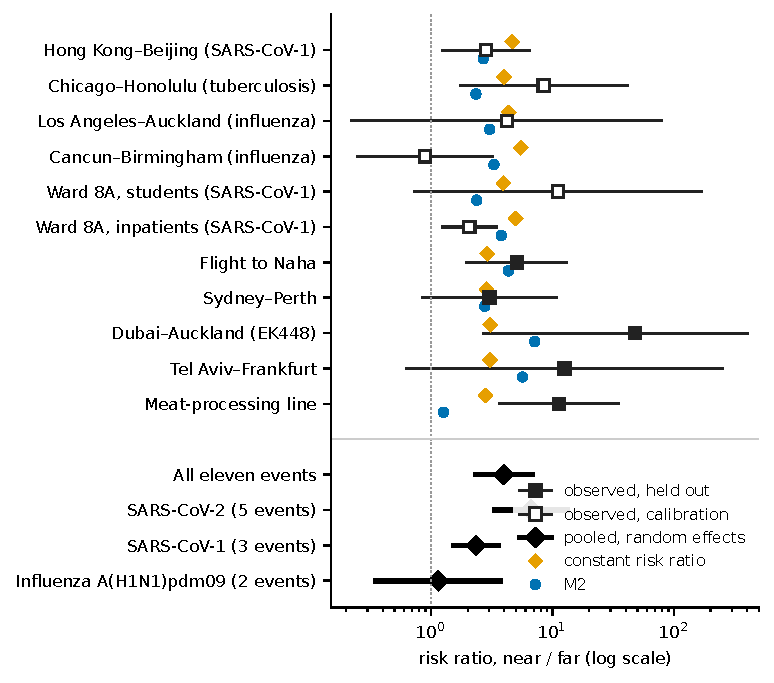
\includegraphics[width=0.82\textwidth]{v2_rr_forest_en}
  % generated by code/v2_figures.py (rr_forest) from data/bsc_validation2/a1_more_outbreaks/07_descriptive.json
  \caption{Near/far risk ratios of the eleven outbreaks of the second dataset, with 95\,\% intervals (a continuity
  correction of 0.5 where a stratum has no case), and random-effects pooled estimates. Near: within two rows
  of a source (aircraft), the index patient's bay or cubicle (ward), within 8\,m (processing line). Small
  symbols: ratio of the expected stratum attack rates under the constant-ratio model and under $\Mtwo$
  (Section~\ref{M-s8_outbreaks:sec:models}; for the six calibration events, from a fit to the other calibration
  events of the class).}
  \label{s8_outbreaks:fig:forest}
\end{figure}

\begin{figure}[tbp]
  \centering
  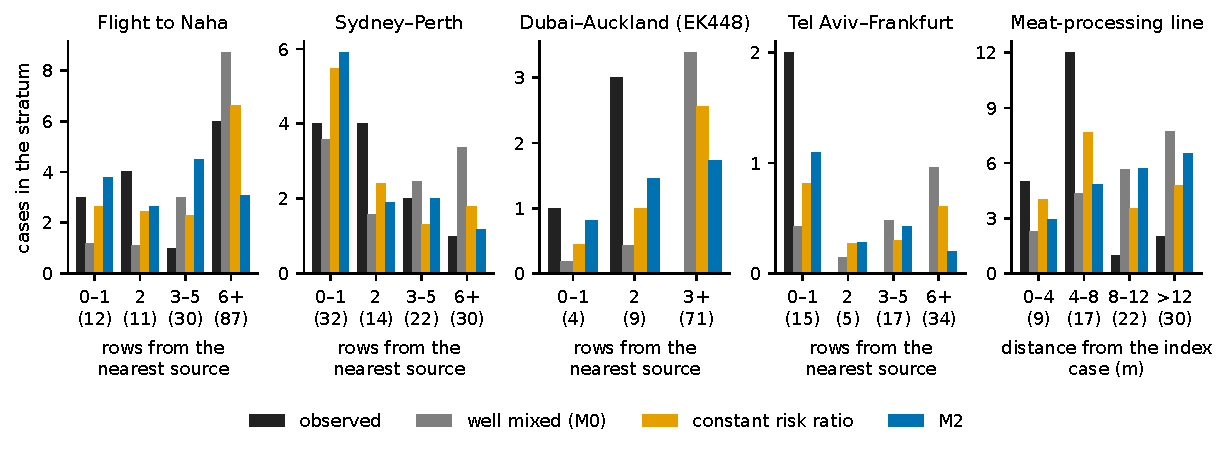
\includegraphics[width=\textwidth]{v2_holdout_strata_en}
  % generated by code/v2_figures.py (holdout_strata) from data/bsc_validation2/a1_more_outbreaks/10_corrected.json (primary_corrected.events)
  \caption{Second test: the five held-out SARS-CoV-2 events. Observed cases by distance stratum and the
  numbers expected, given the event total, under the well-mixed model, the constant-ratio model and $\Mtwo$,
  all calibrated on the six pre-2020 events. In brackets under each stratum: number of people at risk. On the
  four flights $\Mtwo$ and the constant ratio cannot be told apart; on the processing line the constant ratio
  uses a near zone of 8\,m, which the authors of the source selected on these same data.}
  \label{s8_outbreaks:fig:strata}
\end{figure}

Fig.~\ref{s8_outbreaks:fig:strata} shows the observed and expected cases by distance stratum for the five
held-out events. The two ward datasets contradict each other, and no model fits the inpatients in-sample.
% src: code/bsc_validation2/a1_more_outbreaks/PREREG_ADDENDUM_power.md (in-sample adequacy of W2: 0.001-0.025)
The room value is a correction made after the held-out events had been scored. The lattice propagator of the
first test, copied unchanged, loses precision at receivers whose exposure is below its round-off error,
which reaches about $10^{-10}$ of the largest exposure; the room posterior first computed (mode $0.02\sqmh$) came from two such noise values. A
propagator written as a positive sum of image terms removes the defect. The correction changes no number for
the flights, moves the pooled scores from $+13.37$ and $-10.13$ to the values reported below, and leaves the
outcome of the rule unchanged; the re-check confirmed it with a third propagator and found the
restaurant calibration of the first test unaffected (Section~\ref{appS_prot2:sec:numerics}). The hold-out
prediction for the classroom of the first test was affected and is reported corrected
(Section~\ref{M-s8_outbreaks:sec:holdout}).
% src: code/bsc_validation2/a1_more_outbreaks/POSTHOC_LOG.md (P5); data/v2_numbers.json (out2.cal.registered_room_M2: mode 0.020; out2.pooled_registered.M2.all: delta0 13.37, deltaC -10.13); notes/VERIFICATION.md (Section 4.6, second outbreak test, item 13: confirmed)

It is positive in each of the 15 pre-specified
sensitivity variants ($+10.3$ to $+18.1$). These variants were computed with the room kernel as first frozen,
before the numerical correction (primary values $+13.37$ and $-10.13$ with that kernel); the flight parts are
unaffected, and the pooled values would move by about $+1$.

It is significantly in favour of the constant
ratio in the three variants that change the outcome definition of the flights: $-2.52$ (mirror $p=0.013$) with
the confirmed and probable cases of the flight to Naha, $-1.90$ ($p=0.026$) with flight-associated cases only on
the flight from Sydney to Perth, and $-3.42$ ($p=0.005$) with all four changes of outcome definition. It is
significantly in favour of $\Mtwo$, $+1.21$ ($p=0.044$), when the members of two households seated together are
counted once. With the published ratio 2.4 \citep{hertzberg2016risk} in place of the calibrated one $\Mtwo$ is
ahead on the flights ($+1.18$, $p=0.028$) and behind over the five events ($-4.44$, mirror $p=0.002$, with
the room kernel as first frozen; $-4.21$, mirror $p=0.002$, with the re-check's propagator). Comparisons
added during the re-check give $+2.4$ ($p=0.003$) with two strata in place of four, and $+7.8$ and $+2.2$ with a
near zone of one and of five rows. On aircraft $\Mtwo$ is therefore not shown to be better than the two-row rule, nor shown
to be worse; the sign is not determined.

On the
processing line, $p=1.4\times10^{-5}$: the attack rate is flat out to 8\,m (5 of 9, 12 of 17) and then drops (1
of 22, 2 of 30), whereas the ward-calibrated kernel is almost well mixed and expects 2.9, 4.8, 5.7 and 6.5
cases. This is mostly a failure of the transfer from the ward to the line; at the coefficient that the line
itself prefers ($40\sqmh$) the log score of $\Mtwo$ is $-9.5$, still below the $-6.86$ of the constant ratio.

\emph{Secondary analyses of the protocol.} None changes the outcome, and two bear on what follows.
(i)~The kernel of the first test, calibrated on the train cohort ($\Dair\approx20\sqmh$), was applied to the
eight flights with no parameter fitted on any of them. It beats the well-mixed model ($\Delta_0=+7.56$) and is
rejected on four flights ($p=0.020$, 0.004, 0.0002 and 0.015): it is too steep for aircraft, although it
reproduces the two flights whose cases sat next to the sources ($p=0.72$ and 1.0).
(ii)~With the roles exchanged, calibrating on the SARS-CoV-2 events and predicting the earlier ones, $\Mtwo$
beats the constant ratio on the four pre-2020 flights ($\Delta_{\mathrm{C}}=+3.58$, $p=0.004$), because the
ratio learned on the 2020 flights, about 7, over-predicts the earlier gradients, above all on the influenza
flight with none; in the ward it loses ($-3.64$) and fails on the inpatients ($p=2\times10^{-6}$). Pooled,
$\Delta_{\mathrm{C}}=-0.06$.
(iii)~In the 15 sensitivity variants (outcome definitions, sets of sources, row pitch, cabin ventilation,
households, ward calibration) $\Delta_{\mathrm{C}}$ lies between $-12.8$ and $-7.7$ and the outcome is V5 in 12
and V3 (`better than well mixed, but a constant ratio predicts better') in three (kernel as first frozen, see
above).
(iv)~Leaving one event out within each class, $\Mtwo$ and the constant ratio are not separated on the
flights: $\Delta_{\mathrm{C}}=-0.06$, negligible in size but improbable under either model (one-sided
$p=0.046$ under the constant ratio, mirror $p=0.044$ under $\Mtwo$); formally the mirror criterion is met,
but the value is about as improbable under the constant ratio, and the re-check gives $+0.02$; in the rooms $\Mtwo$ is no better than the well-mixed model
($\Delta_0=-0.02$) and the constant ratio predicts better ($\Delta_{\mathrm{C}}=-14.0$).
(v)~Scored seat by seat on the three held-out flights with seat maps, the constant ratio does best ($-76.4$),
ahead of $\Mtwo$ ($-78.6$) and the well-mixed model ($-83.5$).
(vi)~The train kernel of the first test, applied to the rooms, is rejected on the ward inpatients
($p=2\times10^{-5}$) and on the processing line ($p=4\times10^{-4}$).
(vii)~The exploratory two-scale variant of the protocol ($\Mtwo$ plus a well-mixed fraction), evaluated by the
same rule, has $\Delta_0=+17.5$ and $\Delta_{\mathrm{C}}=-5.95$ (mirror $p=2\times10^{-4}$) and fails on the
processing line: outcome V3.
% src: data/v2_numbers.json (out2.sec.train_kernel.posterior: mode 19.95; out2.sec.train_kernel.flights: delta0 7.555; out2.sec.train_kernel.padeq: F1 0.0195, F4 0.0035, F5 0.0002, F6 0.0153, F7 0.72, F8 1.0; out2.sec.swap.air: delta0 6.42, deltaC 3.579, p_B2 0.0039; out2.sec.swap.room: deltaC -3.641; out2.sec.swap_W2: 1.6e-6; out2.sec.swap.all: deltaC -0.063; out2.check.swap.post.air|CRR: mode 7.08; out2.variants.summary: dC -12.78 to -7.65, n_V5 12, n_V3 3; out2.sec.loo_air: deltaC -0.058, p_B2 0.046, p_mirror 0.044; out2.check.loo_air: deltaC +0.018; out2.sec.loo_room: delta0 -0.025, deltaC -14.01; out2.sec.seat: CRR -76.40, M2 -78.62, M0 -83.49; out2.sec.train_kernel.rooms: W2 2.4e-5, P1 4.0e-4; out2.pooled.M3.all: delta0 17.55, deltaC -5.95, p_mirror 0.000215; out2.pooled.M3.decision: B3_failures [P1], outcome V3)

In the second test $\Mone$ was evaluated in its closed form only, as a further column of the same rule. Its
protocol fixed the reading in advance: the first test had shown with the exact simulator that the closed form
overstates the reach of $\Mone$ (on the bus its log score differs from that of the simulated model by 9.9 units,
$-9.58$ against $+0.30$ relative to $\Mzero$; pooled $-11.11$ against $-2.94$), so a pass of the closed form
would not rehabilitate $\Mone$ and a failure would confirm the first test. Against
the well-mixed model it passes with $\Delta_0=+15.45$ over the five held-out events, more than $\Mtwo$ ($+14.35$),
largely through the processing line ($+9.11$ against $+4.16$); against the constant ratio its pooled score is
$\Delta_{\mathrm{C}}=-8.06$ (mirror $p=1.5\times10^{-5}$), as for $\Mtwo$. It fails on three of the five
held-out events (flight to Naha $p=0.008$, flight EK448 $p=0.012$, processing line $p=0.004$), one more than
$\Mtwo$, and on the four flights the constant ratio predicts better ($\Delta_{\mathrm{C}}=-4.63$; a value this
low has probability 0.002 under $\Mone$), where $\Mtwo$ ties. Its formal outcome is the same as that of $\Mtwo$,
V5. Its gain over the well-mixed model is that of an approximation whose error on comparable seated events of
the first test is of the same size, and by the protocol it does not bear on the same-site model; its failures
are consistent with the first test. The same-site model is not supported by the first test, nor, as
Section~\ref{M-s8b_evidence:sec:contacts} shows, by recorded contacts.
% src: data/v2_numbers.json (out2.pooled.M1.all: delta0 15.446, p_B1 0, deltaC -8.055, p_mirror 1.5e-5; out2.pooled.M1.room: delta0 9.115 (out2.pooled.M2.room: 4.158); out2.hold.{F5,F7,P1}.M1.p: 0.0083, 0.0124, 0.0040; out2.pooled.M1.air: deltaC -4.634, p_mirror 0.0017; out2.pooled.M1.decision: B1 true, B2 false, B3_failures [F5, F7, P1], V5; out2.check.M1: air deltaC -4.62, p_mirror 0.0014); code/bsc_validation2/a1_more_outbreaks/PREREGISTRATION.md section 3 (M1cf); data/s8_first_test_exact.json (primary.events.T1: M1cf delta -9.585, M1 +0.297; primary.pooled: M1cf -11.109, M1 -2.939); data/bsc_validation/02b_m1_exact.json (C1 rows: D 0.021-14.93, median 0.2)

The second test confirms this with a test that its protocol lists. For the three room events a common
coefficient is rejected (likelihood ratio 17.4 on 2 degrees of freedom, approximate $p=1.6\times10^{-4}$): the students in
the ward prefer the lower end of the grid, the inpatients about $2{,}000\sqmh$ and the processing line
$40\sqmh$ (16--126). For the eight flights the heterogeneity is weaker (15.2 on 7 degrees of freedom,
approximate $p=0.034$; common value $158\sqmh$, 79--316). These $p$-values, too, use the chi-square reference
although one maximum lies on the edge of the grid and the events have 2 to 20 cases each; the per-event
profiles (Table~\ref{appS_prot2:tab:Dprofiles}) stand regardless. By pathogen the flights prefer $158\sqmh$ for SARS-CoV-2
(63--501), 126 for SARS-CoV-1 (40--794), 16 for tuberculosis (no lower limit) and about 500 for influenza,
where the gain over the largest coefficient of the grid ($10^{4}\sqmh$, close to well mixed) is 0.26 units
of log-likelihood, that is, no detectable gradient
(Table~\ref{appS_prot2:tab:Dprofiles}, Fig.~\ref{appS_prot2:fig:Dprofiles}). Together with the transfer of
the train kernel, which fails on four of eight flights (Section~\ref{M-s8_outbreaks:sec:second}), this leaves
no setting class with a single coefficient, and no transfer between classes.
Section~\ref{M-s8b_evidence:sec:tracer} compares the fitted coefficients with tracer fields, which correspond,
summarised by a diffusion coefficient, to values of order 100 to $1{,}000\sqmh$ in vehicles: far above the
vehicle value calibrated in the first test ($25\sqmh$); its room value, $0.5\sqmh$, is a few hundred times
below the 170 to $185\sqmh$ that a regression on two houses gives for rooms, for which no tracer measurement
exists. The values of the second test are not far below them: the aircraft value, 126, lies inside the range
measured in cabins (112 to 708), and the room value, 794, lies above the regression values. That does not make
an outbreak-fitted coefficient a measurement of air mixing, since within the same test no common coefficient
holds.
% src: data/v2_numbers.json (out2.D.room: LR 17.44, df 2, p 1.63e-4, per_event W1 0.01 (grid edge), W2 1995, P1 39.8 (15.8-125.9); out2.D.air: LR 15.18, df 7, p 0.0338, D_common 158.5, D_common_ci [79.4, 316.2]; by_pathogen: SARS-CoV-2 158.5 (63.1-501.2), SARS-CoV-1 125.9 (39.8-794.3), M. tuberculosis 15.8 (0.01-316), influenza 501 (50-1e4), gain 0.255, measured against the grid end 1e4 (code/bsc_validation2/a1_more_outbreaks/scripts/10_corrected.py: c.max() - c[-1]); out2.check.heterogeneity: room LR 17.67, air LR 15.00; out2.cal.air|M2 125.9; out2.cal.room|M2 794.3; tr.D.cabin: 112, 708; tr.D.table: classroom 169, office 185)

\subsection{Recorded contacts}\label{s8b_evidence:sec:contactsdetail}

\begin{table}[tbp]
  \centering\small
  \caption{Contacts generated by each model against RFID contact records in six indoor settings (calibrated on
  the first half of the days, scored on the second half). Families: number of the seven families of contact
  statistics passed, per dataset, in the order office 2013, primary school, hospital ward, office 2015, high
  school, conference (six families apply at the conference, which has no groups). Scenarios: SIR scenarios
  passed, of 24 (four per dataset). Ratio: secondary cases of the index case on model contacts divided by
  those on the recorded contacts, range over datasets of the mean over scenarios. Last column: mean absolute
  error of the attack rate over the 24 scenarios. The first four rows are the pre-specified test; the others
  are not.}
  \label{s8b_evidence:tab:contacts}
  % generated: data/v2_tab_contacts.tex (code/v2_numbers.py <- data/bsc_validation2/a2_contact_mobility/*.json, code/checks/contacts/check_summary.json)
  \begin{tabular}{@{}>{\raggedright\arraybackslash}p{0.34\textwidth}c>{\centering\arraybackslash}p{0.17\textwidth}ccc@{}}
    \toprule
    Model & Parameters & Families passed (of 7) & Scenarios & Ratio & Error \\
    \midrule
    \tabinput{data/v2_tab_contacts}
    \bottomrule
  \end{tabular}

  \smallskip
  \begin{minipage}{0.96\textwidth}\footnotesize
  $^{a}$\,Added post hoc during the re-check: contact rate of each pair taken from the training days, no space;
  exploratory.
  $^{b}$\,Developed on the first three datasets after the walk had failed on them; description after the fact
  (the confirmatory test on the last three datasets was uninformative).
  \end{minipage}
\end{table}

Two things are scored on the test days. \emph{Structure}: seven families of contact statistics (total contact
time; contact durations; gaps between contacts and recurrence of pairs; number of partners; heterogeneity
between people; repetition of pairs from one day to the next; share of contact within groups), each passed if
the model lies within a factor 0.8 to 1.25 of the data, or within a stated absolute margin. \emph{Epidemic
consequence}: an SIR epidemic is run on the recorded temporal network of the test days and on the
model-generated contacts, at the same total contact time, in four scenarios (nominal reproduction number 1.5
or 3; infectious period 1 or 4 days); a scenario is passed if the secondary cases of the index case agree
within 10\pct{} and the probability of a major outbreak and the mean attack rate within 0.05, and the epidemic
criterion is met with three of four scenarios. The rule: the movement component is validated on a dataset if
it meets the epidemic criterion and at least six of the seven families, and overall if it does so on
two-thirds of the datasets; the outcome is called A0 if it neither does this nor meets the epidemic criterion
where the well-mixed model fails. On synthetic data a true model passed in 20 of 20 replicates and a wrong one
reached the per-dataset criterion in none of 44. The protocol recorded the expectation A0.
% src: code/bsc_validation2/a2_contact_mobility/PREREGISTRATION.md sections 5-7; code/bsc_validation2/a2_contact_mobility/POSTHOC_LOG.md item 1 (0 of 44); data/v2_numbers.json (con.power.cells)

\begin{figure}[tbp]
  \centering
  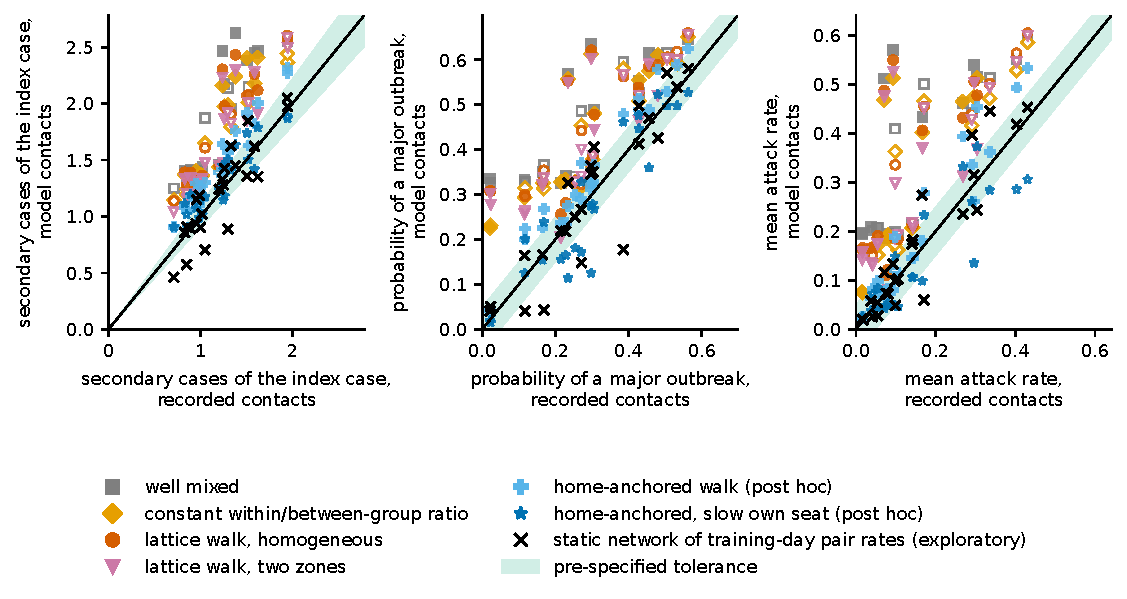
\includegraphics[width=\textwidth]{v2_contacts_epidemic_en}
  % generated by code/v2_figures.py (contacts_epidemic) from data/bsc_validation2/a2_contact_mobility/{s1,s2b,s2d,s3a,s3b,s3d}_<dataset>.json (epi) and verify/v4_static_*.json
  \caption{SIR outcomes on model-generated contacts against the same outcomes on the recorded contacts of the
  test days: six datasets, four scenarios each. Open symbols: the three development datasets; filled: the
  three confirmatory ones. Shaded: tolerance of the protocol. Points above the diagonal are over-predictions.
  The lattice walk, in both forms, lies with the two models without space; the walks anchored to home sites
  were developed after that failure, and the static network was added during the re-check.}
  \label{s8b_evidence:fig:contacts}
\end{figure}

\paragraph{Result: the walk fails on all six datasets.}
The homogeneous walk passes one or two of the seven families on each dataset, namely those it was calibrated
on, the total contact time and the mean duration; the two-zone walk passes two on each
(Table~\ref{s8b_evidence:tab:contacts}; Fig.~\ref{appS_prot2:fig:structure}). What it does not reproduce is
who meets whom. People in the walk have too many partners on five of the six datasets: 6.0 per person and day
against 4.6 in the office of 2013, 34 against 15 in the high school, 90 against 47 in the primary school.
Contact within the recorded groups is 10 to 33\pct{} of contact time in the walk and 57 to 94\pct{} in the
data. Long contacts, the burstiness of the gaps between contacts (0.08--0.25 against 0.36--0.61) and the
repetition of the same pairs on the next day are missing as well. The real training days, used as a predictor
of the test days, reproduce the burstiness on all six datasets, the long contacts on four (not in the office of
2013 and the hospital ward) and the repetition of pairs on three of the four datasets where it is defined (not
in the hospital ward; it is undefined at the primary school and the conference).
% src: data/v2_numbers.json (con.model.RW0.S: [1,2,2,1,1,1]; con.model.RWhet.S: [2,2,2,2,2,2]; con.stats_obs_vs_RW0: S3_deg_mean 4.58/5.96 (InVS13), 14.6/33.8 (Thiers13), 46.6/90.4 (LyonSchool), 26.5/23.4 (SFHH); S6_within_frac observed 0.57-0.94, walk 0.10-0.33; S2_burst observed 0.36-0.61, walk 0.08-0.25; con.realtrain_S: [6,6,4,6,6,4]); data/bsc_validation2/a2_contact_mobility/s1_{InVS13,LyonSchool,LH10}.json and s3a_{InVS15,Thiers13,SFHH}.json (models.REALtrain.score: S2_intercontact true on all six; S1_duration false for InVS13, LH10; S5_persistence false for LH10, null for LyonSchool, SFHH)

The consequence for an epidemic is systematic. Because the walk spreads the same contact time over too many,
too equal partners, the index case infects more people on the walk's contacts than on the recorded ones in
all 24 scenarios, by 15 to 86\pct{}, and by 25 to 72\pct{} on average per setting; the mean attack rate is too
high by 0.10 to 0.29 (Fig.~\ref{s8b_evidence:fig:contacts}). No scenario is passed on any dataset. The total
contact time of model and data agrees within 2.5\pct{} in these runs, so the excess is not an artefact of the
contact rate. The re-check reproduced the result with its own data loader, walk simulator and
epidemic code, on files downloaded again from the source.
% src: data/v2_numbers.json (con.model.RW0: E_scen [0,0,0,0,0,0], n_cells_over 24 of 24, ratio_cell_min 1.151, ratio_cell_max 1.860, ratio_min 1.253, ratio_max 1.715, dA_per_dataset 0.103-0.292, contact_time_ratio 0.977-1.009); notes/VERIFICATION.md (Section 4.7, contact records, items 2, 3: confirmed)

The two models without space do neither better nor worse: both pass no scenario, with ratios of 1.25 to 1.79
(well mixed) and 1.20 to 1.63 (constant group ratio). The outcome is A0, with the sentence that the protocol
reserved for this case: the lattice walk adds nothing over a non-spatial contact model. The conclusion is, if
anything, understated. A static network with no space and no walk, in which each pair keeps the contact rate
it had on the training days, meets the epidemic criterion on three of the six datasets and passes 12 of the 24
scenarios, where neither pre-specified walk meets it on any dataset (the anchored walk with a slow own seat,
designed afterwards on the development datasets, meets it on one of them). This comparison was added during the
re-check after the results were known, with a crude estimator whose contact time is 2 to 9\pct{} low, so it is exploratory; and the
tolerance is tight, since the real training days used as a predictor of the test days meet the criterion on
four of the six datasets only. Neither point touches the result for the walk, whose error is several times
the tolerance.
% src: data/v2_numbers.json (con.model.WM: ratio 1.248-1.793, scen_total 0; con.model.BLOCK: 1.201-1.631, 0; con.ladder: A0 for every model; con.check.static: scenarios 0,4,0,3,2,3 -> 12 of 24, 3 of 6 datasets; con.model.RW0.E_datasets 0, con.model.RWhet.E_datasets 0, con.model.RWstickO.E_scen [0,0,3,2,0,0], E_datasets 1; con.check.train_replay: 2,4,4,3,1,4 -> 4 of 6 datasets); notes/VERIFICATION.md (Section 4.7, contact records, items 6 and 9)

One further property is against the mass-action picture of the model. In the walk, as in the well-mixed
model, the number of contacts grows as the square of the number of people present (fitted exponents 1.95 to
2.20). In the data the exponent is 0.45, 0.95, 0.76 and 0.81 in the two offices, the high school and the
conference, and 2.8 in the hospital ward: in four of five settings a person's contact rate does not grow
with occupancy. This comparison is descriptive: occupancy varies with the time of day, so the exponent
mixes density with schedule, and 20-minute intervals without a contact were left out of the fit, which biases
the observed exponent on the sparse datasets.
% src: data/v2_tab_datasets.tex (S7_alpha observed / walk: 0.45/1.97, 2.83/2.20, 0.95/2.06, 0.76/2.12, 0.81/1.95; primary school not comparable, occupancy range 1.27 < 1.5); notes/VERIFICATION.md (Section 4.7, contact records, item 7: partially confirmed; further point 9: bins with zero contacts dropped)

\paragraph{Walkers anchored to home sites: neither supported nor refuted.}
The protocol provided for a second stage. On the three development datasets the smallest changes that repair
the failed families were sought, keeping a Markov walk with same-site contact: a home site for each person
with a drift towards it, homes of the same group clustered in space, and either a slow seating zone, which is
the heterogeneous mobility $D_x$ of the model, or a walker that is slow on its own seat only, which is not.
The three variants, with their automatic fitting procedure, were frozen before the three confirmatory datasets
were touched. On those datasets none meets the epidemic criterion (the variant with a slow own seat passes
2, 0 and 0 of 4 scenarios; the variant with a slow seating zone passes none of 12), and the formal outcome is
again A0.
% src: code/bsc_validation2/a2_contact_mobility/POSTHOC_LOG.md items 3-13; code/bsc_validation2/a2_contact_mobility/FIX_FREEZE.json; data/v2_numbers.json (con.model.RWstickO.E_scen: [0,0,3,2,0,0]; con.model.RWstickZ.scen_conf 0; con.model.RWclus.scen_conf 0)

This outcome must not be read as a test that anchoring failed. In the re-check synthetic
contact data were generated from the anchored models themselves and the frozen fitting procedure was applied to
them: it failed
the epidemic criterion in six of seven replicates, with degenerate fits in four. A procedure that cannot
recover its own truth cannot refute a model, so the confirmatory stage is uninformative. What remains is a
description made after the fact. Over all 24 scenarios the mean absolute error of the attack rate falls from
0.17 for the homogeneous walk to 0.04--0.05 for the anchored variants, and the error of the index case's
secondary cases by 47 to 70\pct{}; two of the three variants still over-predict the secondary cases in all 24
scenarios, by 6 to 36\pct{}. These figures use the recorded group labels and are not at matched contact
time: the ratio of model to recorded contact time is 0.96 to 1.05 and 0.92 to 1.06 for the two variants with
clustered homes, and 0.98 to 1.11 for the variant with a slow own seat except in the high school, where it is
2.34; the reduction of 70\pct{} belongs to that variant and includes the high school. They indicate a
direction, home anchoring with clustered homes, and are not a result; no variant reproduces burstiness or the
repetition of pairs between days. A random walk in which people slow down near attractive individuals was
proposed and compared with SocioPatterns records by \citet{starnini2013modeling}; the anchored walks found here
by trial are close to that idea, and what is added is the epidemic consequence and the comparison with models
without space.
% src: notes/VERIFICATION.md (Section 4.7, contact records, items 4, 5; further points 1, 4, 5); data/v2_numbers.json (con.check.self_power; con.model.RW0.mean_abs_dA 0.167, mean_abs_log_ratio 0.361; con.model.RWclus: 0.041, 0.191, ratio_cell 1.07-1.36, n_cells_over 24; con.model.RWstickZ: 0.038, 0.166, 1.06-1.35, 24; con.model.RWstickO: 0.050, 0.108, n_cells_over 17; contact_time_ratio: RWclus 0.960-1.052, RWstickZ 0.917-1.058, RWstickO 0.983-1.109 and 2.340 (Thiers13); 1 - 0.108/0.361 = 0.70)

\paragraph{Scope.}
The result holds for one identification of the walk: a site is a contact range, steps are synchronous, and the
lattice has as many sites as the contact rate requires. The calibrated hop probabilities, 0.20 to 0.42 per
20-second step, correspond to a mobility of about 220 to 450 sites$^2$ per day if a site is identified with a
cell of Section~\ref{M-s2_model:sec}: between $\Dz=1\cellday$, which was not tested against contacts, and walking
mobility. Other site sizes and the continuous-time walk were not tried. The size of the over-prediction depends on the design with a nominal reproduction number, which
forces a high transmission probability per contact interval on sparse datasets; it is smallest in the primary
school (ratios 1.15 to 1.34). The sensors record proximity, not position, so the occupancy of zones could not
be tested, and neither could a measured mobility field.
% src: notes/VERIFICATION.md (Section 4.7, contact records, further points 6, 7); code/bsc_validation2/a2_contact_mobility/POSTHOC_LOG.md item 17; data/v2_numbers.json (con.dataset.*.p: 0.203-0.417; per-direction hop rate (p/4) x 4,320 steps per day = 219-451; data/bsc_validation2/a2_contact_mobility/s1_LyonSchool.json (epi.*.RW0.R_index / epi.*.REAL.R_index: 1.151, 1.321, 1.204, 1.337, ratios computed from the stored values)); code/bsc_validation2/a2_contact_mobility/PREREGISTRATION.md section 3 (move to a uniformly chosen neighbour accepted with probability p per 20 s step)

\subsection{Tracer measurements}\label{s8b_evidence:sec:tracerdetail}

\begin{table}[tbp]
  \centering\footnotesize
  \setlength{\tabcolsep}{3.4pt}
  \caption{The kernel fixed by tracer measurements, with nothing fitted to outbreaks except one
  $\varepsilon_k$ per event, on the stratum events of the first dataset. RR: predicted and observed near/far risk
  ratio; $p$: two-sided predictive $p$ of the observed near count under the tracer kernel and under
  $\Mzero$; last three columns: log score of the tracer kernel minus that of $\Mzero$ and of the constant
  ratios 2 and 3.}
  \label{s8b_evidence:tab:tracer}
  % generated: data/v2_tab_tracer.tex (code/v2_numbers.py <- data/bsc_validation2/a3_tracer_physics/04_evaluation.json)
  \begin{tabular}{@{}lccccccc@{}}
    \toprule
    Event & Near vs far & RR pred.\ / obs. & $p$ & $p$, $\Mzero$ & $-\Mzero$ & $-$ratio 2 & $-$ratio 3 \\
    \midrule
    \tabinput{data/v2_tab_tracer}
    \midrule
    Pooled & & & & & $+7.87$ & $-0.80$ & $-0.78$ \\
    \bottomrule
  \end{tabular}

  \smallskip
  \begin{minipage}{0.96\textwidth}\footnotesize
  $^{a}$\,With a continuity correction (no case at the remote tables). $K$: number of cases counted as
  acquired at the two neighbouring tables; with the source's own count, $K=5$, the tracer kernel is rejected
  ($p=0.002$).
  \end{minipage}
  % src: data/v2_numbers.json (tr.pooled_sum: M0 +7.873, CRR2 -0.800, CRR3 -0.780; tr.restaurant_byK: P 0.095, 0.027, 0.0074, 0.0019 for K = 2..5)
\end{table}

\paragraph{Measured mixing coefficients.}
If the non-local term of $\Mtwo$ describes the transport of aerosol, its mixing coefficient can be measured
without any outbreak, by releasing a tracer and recording its concentration. Published measurements exist for
four of the settings of Section~\ref{M-s8_outbreaks:sec}: ethane tracer gas at eight seats of the Hunan coach
itself, with a tracer-validated flow simulation for all seats \citep{ou2022}; fluorescent 1\,\textmu m particles
released from a breathing mannequin in the forward cabin of a wide-body aircraft \citep{kinahan2021aerosol};
salt aerosol along the saloon of an inter-city rail carriage \citep{woodward2022evaluation}; and tracer gas at
seven tables of the Guangzhou restaurant, with the source's flow simulation at the others \citep{li2021}. For the classroom and the open-plan office no
measurement exists, and the coefficient was taken from a regression of the turbulent diffusion coefficient on
the air change rate measured in two houses \citep{cheng2011modeling}, whose measured values are 3.6 to
$47\sqmh$ at below 0.2 to above 5 air changes per hour; it is extrapolated to rooms of several hundred cubic
metres at 2 to 12 air changes per hour. The estimators were fixed
before any coefficient was computed: a least-squares fit of the logarithm of the steady concentration of
$\Mtwo$ to the logarithm of the tracer reading, on the lattice of the event.
% src: code/bsc_validation2/a3_tracer_physics/PREREGISTRATION.md section 3; data/tracer/SOURCES.md (Cheng et al. 2011: K from 0.001 to 0.013 m2/s, i.e. 3.6 to 46.8 m2/h); data/v2_numbers.json (tr.D.table: classroom 429 m3, 2-12 ACH, 169 (38-745))

\begin{figure}[tbp]
  \centering
  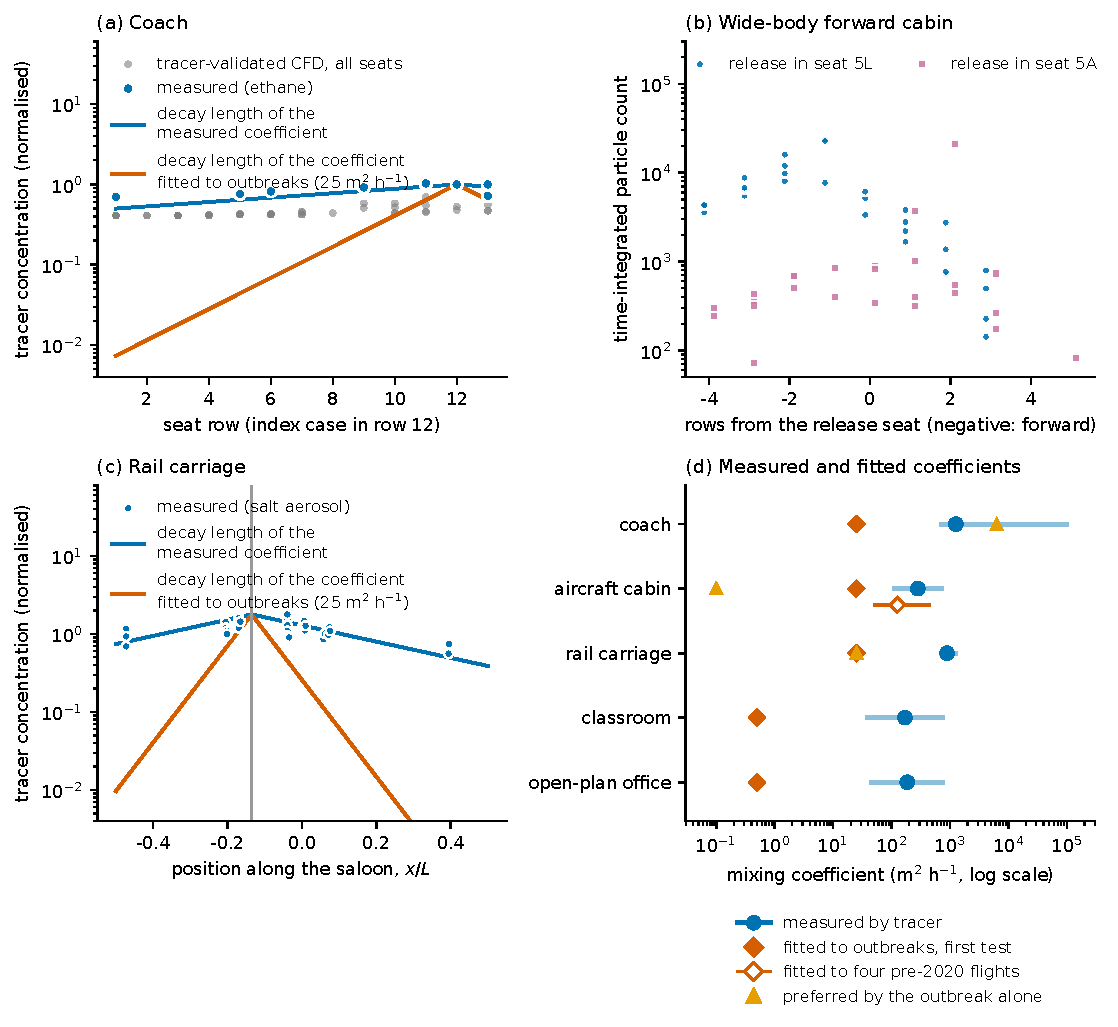
\includegraphics[width=\textwidth]{v2_tracer_kernels_en}
  % generated by code/v2_figures.py (tracer_kernels) from data/tracer/{ou2022_B1_seats.csv, kinahan_tidy.csv, woodward2022_fig9_points.csv}
  % and data/bsc_validation2/a3_tracer_physics/{01_kernels.json, 05_descriptive.json}; data/bsc_validation2/a1_more_outbreaks/10_corrected.json (primary_corrected.post.air|M2)
  \caption{Tracer measurements. (a)~Coach of the Hunan outbreak: ethane measured at eight seats and the
  tracer-validated flow simulation at all seats \citep{ou2022}. (b)~Forward cabin of a wide-body aircraft:
  time-integrated particle counts by row for two releases, zero readings not shown
  \citep{kinahan2021aerosol}. (c)~Rail carriage: salt aerosol along the saloon, release at the vertical line
  \citep{woodward2022evaluation}; points digitised from the published figure. The lines in (a) and (c) are
  exponentials with the decay length $\sqrt{\Dair/\remrate}$ of the measured coefficient and of the $25\sqmh$
  fitted to the train cohort; they illustrate the two length scales and are not the fitted lattice fields.
  (d)~Mixing coefficients: measured (with range), fitted to outbreaks in the first test, fitted to the four
  pre-2020 flights of the second test (with 90\,\% interval), and preferred by the outbreak of that setting
  taken alone.}
  \label{s8b_evidence:fig:kernels}
\end{figure}

In the three vehicles the measured fields, summarised by a diffusion coefficient, are of order 100 to
$1{,}000\sqmh$ (Fig.~\ref{s8b_evidence:fig:kernels}d): $1{,}259$ in the coach (5th percentile of a bootstrap 708;
the eight points are nearly flat and bound the coefficient from below only), 708 and 112 for the two releases
in the cabin (geometric mean 282), and 891 and 355 for a release in the middle and at the end of the carriage.
For the classroom and the office no tracer measurement exists, and no coefficient was derived from the
restaurant's readings, which enter as a kernel directly; the regression extrapolated to the volume and
ventilation of the classroom and the office gives about 170 to $185\sqmh$ (38 to 753). The coefficients fitted to outbreaks in the
first test are $25\sqmh$ for vehicles and $0.5\sqmh$ for rooms, and the flight VN54 alone prefers 0.06 to 0.1.
The measured vehicle values are thus 4.5 to about 50 times the vehicle value of the first test, and the
extrapolated room values a few hundred times its room value. The second test is different: its aircraft
coefficient, $126\sqmh$ (52--438), lies inside the range measured in cabins, and its room coefficient, $794\sqmh$
(302--4{,}390), lies above the extrapolated room values. Three reservations on the cabin value: the fit uses positive
readings only, and estimators that keep the zero readings give 56 to $450\sqmh$; the two fits move from 708
and 112 to 891 and $178\sqmh$ if four additional sensors, one of them with an outlying reading, are left out;
and the measured field is not diffusive (it is biased forwards and cut off aft of row 8), so that a single
coefficient summarises it loosely.
The decay lengths $\sqrt{\Dair/\remrate}$ are about 2 to 5\,m in the cabin and 5 to 14\,m in the carriage and
the coach.
% src: data/v2_numbers.json (tr.D.coach: D 1259, lo 708; tr.D.cabin: D_5L 708, D_5A 112, D_geomean 282; tr.D.train: middle 891, end 355, len 8.3, 5.2; tr.D.table: classroom 169, office 185, coach length 13.9, cabin length 2.8; out2.cal.air|M2: 126, 52-438; out2.cal.room|M2: 794, 302-4391; tr.D.table: classroom 169 (38.4-745.2), office 185 (45.6-753.0)); data/checks/tracer.json: cabin_D (56-450 with zeros kept; 112 -> 178 and 708 -> 891 without the four additional sensors), cabin_decay_lengths_m (1.8-4.5), ratio_tracer_to_outbreak_D_at_low_cabin_value (4.5); notes/VERIFICATION.md (Section 4.8, tracer measurements, item 12; further point 3: field not diffusive; further point 4)

\begin{figure}[tbp]
  \centering
  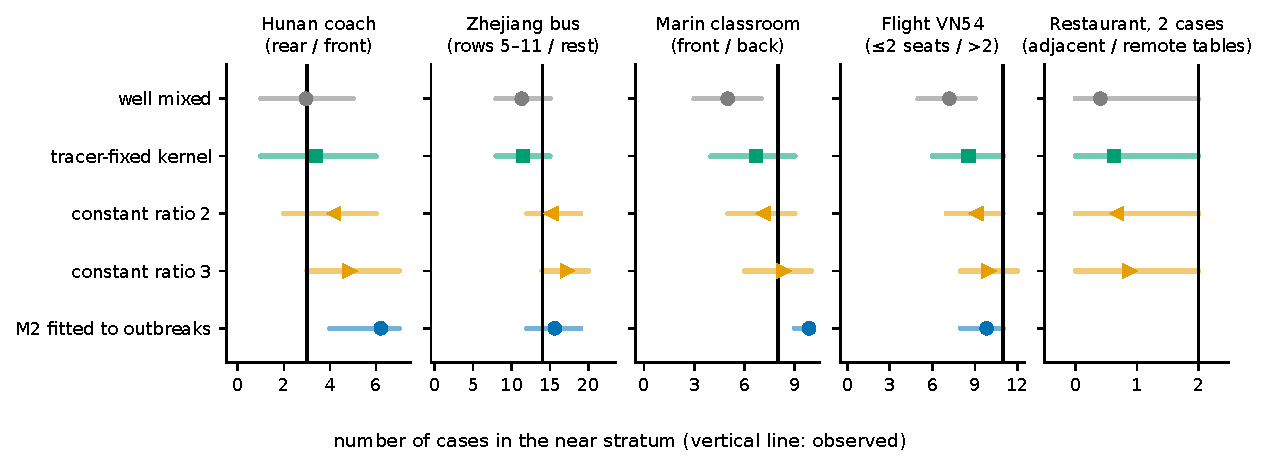
\includegraphics[width=\textwidth]{v2_tracer_predictions_en}
  % generated by code/v2_figures.py (tracer_predictions) from data/bsc_validation2/a3_tracer_physics/04_evaluation.json (events.*.models.*: mean_near, int95)
  \caption{Number of cases in the near stratum, given the event total: mean and 95\,\% predictive interval
  under the well-mixed model, the kernel fixed by tracer measurements, the constant ratios 2 and 3, and
  $\Mtwo$ with the coefficient fitted to outbreaks in the first test (at its posterior mode; the restaurant was
  a calibration event). The tracer kernel removes the over-prediction on the coach by coming close to the
  well-mixed model. The gradients of flight VN54 and of the restaurant are not reproduced: the formal
  non-rejection of the flight depends on zero sensor readings (see text), and the restaurant is shown at the
  lower bound of its case count.}
  \label{s8b_evidence:fig:tracerpred}
\end{figure}

\paragraph{Confronted with the outbreaks.}
With the kernel fixed in this way, the seven events of the first dataset were predicted with one free parameter
each, the infectiousness (Table~\ref{s8b_evidence:tab:tracer}, Fig.~\ref{s8b_evidence:fig:tracerpred}). The
trains and the restaurant, calibration records before, are test events here.

\emph{Coach and call centre: no longer rejected, and not informative.} For the coach the measured kernel
predicts a rear/front ratio of 1.29 where 1.03 was observed ($p=1.00$); the kernel fitted to outbreaks had
predicted 11. For the call centre it predicts little desk-scale clustering, and the probability of a join-count
$z$ as small as observed is 0.10 (Fig.~\ref{s8_outbreaks:fig:callcentre}c). In both cases the measured kernel
is close to the well-mixed model, which fits as well or better ($p=1.00$ and 0.26); for the call centre the
kernel still predicts clustering of the wrong sign (median $z=+0.78$ against $-0.64$ observed). The two
failures of Section~\ref{M-s8_outbreaks:sec:holdout} are removed only in the sense that the model has stopped
predicting a gradient.
% src: data/v2_numbers.json (tr.event.T2: P p 1.0, rr_expected 1.285, M0 p 1.0, M2cal_mode p 0.0029; tr.callcentre: P P_le_obs_pooled 0.101, median 0.785; M0 0.258; z_obs -0.645); notes/VERIFICATION.md (Section 4.8, tracer measurements, items 4, 5)

\emph{Bus: inconclusive.} Predicted ratio 1.03 against 1.60 observed, $p=0.22$; the well-mixed model has
$p=0.20$.
% src: data/v2_numbers.json (tr.event.T1: P p 0.217, rr_expected 1.033; M0 p 0.204)

\emph{Classroom: the one gain.} The room relation predicts a front/back ratio of 1.77 where 2.8 was observed
($p=0.42$), and the well-mixed model is rejected ($p=0.036$). The result holds when the coefficient is doubled
or halved and under two other dose--response laws, and the implied emission, 317 quanta per hour (173--642),
lies within the range of the single events of Table~\ref{s8_outbreaks:tab:levels}, unlike the median
$8\times10^{7}$ that the first test needed. Constant ratios of 2 and 3 do as well, and the coefficient is
extrapolated from two houses, with the teacher's position assumed.
% src: data/v2_numbers.json (tr.event.C1: P p 0.424, rr_expected 1.769, M0 p 0.036, KB_Dx2 0.223, KB_Dhalf 1.0, P_lin 1.0, P_gam 0.228, CRR2 0.663, CRR3 1.0; tr.emission."C1 classroom": [172.9, 317.5, 642.2])

\emph{Flight VN54: not reproduced.} The predicted ratio is 1.66 against 7.3 observed: with 11 of 12 near
passengers infected and 1 of 8 far, the exponential dose--response law needs a dose ratio of about 19, and the
measured kernels give 1.5 to 3.9. The formal test does not reject ($p=0.14$), but only because the predictive
distributions of two releases that contradict each other are averaged, and because three sensors that map onto
far seats read exactly zero in one of them. With the zeros treated as missing, a variant listed in the
protocol, $p=0.003$; the flight is rejected in four of the six listed variants. The tracer tests were made in
another airframe.
% src: data/v2_numbers.json (tr.event.T5: P p 0.136, rr_expected 1.660, KA_5L 0.0007, KA_5A-mirrored 0.229, KA_zeros_missing 0.0028, KB_measD 0.045, KB_measD_oldvent 0.029, P_gam 0.0496, P_lin 0.185; tr.dose_ratio.T5: 18.6); data/bsc_validation2/a3_tracer_physics/01_kernels.json (cabin.*.direct.*.near_far_mean_ratio: 1.49-3.86); code/bsc_validation2/a3_tracer_physics/POSTHOC_LOG.md (P4); notes/VERIFICATION.md (Section 4.8, tracer measurements, item 8: to be reported as not reproduced)

\emph{Restaurant: not reproduced at the reported count.} The tracer concentration at the 13 remote tables
was on average 0.55 of that at the index table (0.32 to 0.86); four of these values are measured and nine are
the source's flow simulation, the lowest among them. With two cases counted as acquired at the neighbouring tables
the kernel is not rejected ($p=0.095$); with the five that the source reports, against none among 63 remote
patrons, it is ($p=0.002$).
% src: data/v2_numbers.json (tr.restaurant_tracer: remote_mean 0.553, 0.32-0.86; tr.restaurant_byK: 0.095, 0.027, 0.0074, 0.0019); data/bsc_outbreaks/tables/li2021_restaurant_tables.csv (norm_measured_tracer at TB, TC, T10, T15, T16, T17, T18; norm_predicted_tracer used elsewhere, code/bsc_validation2/a3_tracer_physics/src/a3lib.py r1_tables; remote minimum 0.32 at T09, simulated)

\emph{Trains: failure.} The kernel measured in the carriage is nearly flat over three rows and expects 14.6
cases in the row of the index case where 50 were observed (deviance 112.8 on 21 degrees of freedom,
$p<0.0005$). Every model fails on this table: the well-mixed model (125.6), constant ratios of 2 and 3 for the
index row (81.5 and 64.1) and the kernel that was fitted to the table in the first test (72.3).
% src: data/v2_numbers.json (tr.trains: P deviance 112.83, M0 125.61, CRR2 81.51, CRR3 64.06, M2cal_mode 72.30; tr.trains_rows.0: k 50, P 14.56)

\emph{Pooled.} Over the five stratum events the tracer kernel scores $+7.87$ against the well-mixed model
(exact one-sided $p=1.4\times10^{-6}$; $+3.41$ without the flight) and $-0.80$ and $-0.78$ against the constant
ratios 2 and 3, which themselves beat the well-mixed model by more ($+8.67$ and $+8.65$). The outcome of the
rule is S4, one adequacy failure (the trains) and no gain over the generic gradient; on the defensible reading
of the flight it is S5, two failures. The formal outcome S4 does not discriminate between the truths considered
in the power analysis (Table~\ref{appS_prot2:tab:tracerrule}, Section~\ref{appS_prot2:sec:tracer}). A
comparison added during the re-check, after the results were known, gives the probability of the pooled pattern
alone (better than well
mixed, not better than both constant ratios): 0.23 if the tracer kernel is true, 0.84 under a constant ratio of
2 and about 1.00 under a ratio of 3, so that the pooled evidence favours a generic ratio over the kernel by a
factor of about four (3.7 to 4.4).
% src: data/v2_numbers.json (tr.eval.pooled.P: M0 delta 7.873, p 1.44e-6; CRR2 -0.800; CRR3 -0.780; tr.crr_vs_M0: 8.673, 8.653; tr.eval.decision: outcome S4, D1_failures [T4]; tr.pooled_without.pooled_P_vs_M0_without_T5: +3.411); data/v2_numbers.json (tr.power.pattern: P_D2_not_D3 P 0.229, CRR2 0.842, CRR3 0.997; ratios 3.68, 4.36; enumerated by code/v2_numbers.py from data/bsc_validation2/a3_tracer_physics/02_predictions.json); data/checks/tracer.json: pooled_pattern_probability (0.23 / 0.84 / 1.00); notes/VERIFICATION.md (Section 4.8, tracer measurements, item 11: outcome S5 if the flight is counted as a failure)

\paragraph{An exploratory extension to four flights.}
After these results were known, the same cabin coefficients (112 and $708\sqmh$, equal weights) were applied
to the four held-out flights of Section~\ref{M-s8_outbreaks:sec:second}. The extension has a protocol of its
own, written with the near/far counts and the outcome of the second outbreak test known, and it reverses two
exclusions of the main protocol; it is exploratory and takes no part in any decision. The tracer kernel is not
rejected on any of the four flights ($p=0.054$, 0.26, 0.25 and 1.00), scores $+10.4$ against the well-mixed
model and $+2.8$ against a constant ratio of 2 ($p=0.005$), and ties with a ratio of 3 ($-0.16$). The absence
of a rejection is at the edge: with the geometric-mean coefficient that the main protocol specifies, the
flight to Naha is rejected ($p=0.044$), and each of the two coefficients taken alone fails one flight
($p=0.025$ and 0.002). The tracer measurements were made in wide-body cabins, and two of the four flights
were on Boeing~737 aircraft (Table~\ref{appB_dataset:tab:second}), so the transfer of the coefficient is
itself untested. What survives, as an exploratory result, is small: the two cabin coefficients (112 and
$708\sqmh$), measured without any outbreak, beat the well-mixed model and tie with a constant ratio of 3.
% src: data/v2_numbers.json (tr.ext.events.*.models.P.p: 0.054, 0.260, 0.246, 1.0; P_D708 on F7: 0.025; P_D112 on F5: 0.0016; tr.ext.pooled.P: M0 +10.36, CRR2 +2.83 (p 0.005), CRR3 -0.16); code/bsc_validation2/a3_tracer_physics/PREREG_EXT_flights.md section 0; data/checks/tracer.json: extension_naha.p_with_single_geometric_mean_D (p = 0.044, D = 282); notes/VERIFICATION.md (Section 4.8, tracer measurements, item 13; further point 9: tracer data are wide-body only); data/v2_tab_events2.tex (F5 B737-800, F8 B737-900)

\paragraph{Reading.}
Measured mixing is fast. A kernel with the measured coefficient is therefore close to well mixed in the coach
and the carriage and mild in the rooms, and it cannot produce the steep gradients of the train cohort, of
flight VN54 or of the restaurant. Those gradients need something other than diffusion at the scale of the
enclosure: exposure within about a metre, companions, directed airflow. The tracer kernel is not validated as
a spatial predictor; its one gain over the well-mixed model, the classroom, is matched by a constant ratio.
Only the coach and the restaurant have a tracer test in the enclosure of the outbreak; the cabin, the carriage
and the rooms rest on transfers that are themselves untested.
% src: notes/VERIFICATION.md (Section 4.8, tracer measurements, summary; further point 9)

\subsection{Zone-level structure}\label{s8b_evidence:sec:zonesdetail}

\begin{table}[tbp]
  \centering\small
  \caption{Zone-level test: influenza in 29 primary schools, with mixing shares measured in another school.
  Differences are of held-out log-likelihood (two-fold cross-validation by school), with 95\,\% bootstrap
  intervals over schools. The last two rows are post hoc, added during the re-check.}
  \label{s8b_evidence:tab:zone}
  % src: data/v2_numbers.json (zone.D_Z_minus_H: 798.4 [561.9, 1072.5]; zone.D_Z_minus_X: 211.1 [109.8, 340.4]; zone.D_Z_minus_C: 18.8 [-8.8, 54.0]; zone.primary_other: w_hat [0.659, 0.104, 0.236], LR_F_vs_Z 42.71, TV 0.1028, disp_obs 3.383, disp_pred_Z [2.65, 3.17, 3.61]; zone.TV_boot_ci [0.047, 0.168]; zone.check.hazard_bound."1e-09".D_N702: -19.1 [-37.8, -3.3]; zone.check.D_Z_minus_H: 744.8 [530.7, 999.0])
  \begin{tabular}{@{}>{\raggedright\arraybackslash}p{0.47\textwidth}>{\raggedright\arraybackslash}p{0.27\textwidth}>{\raggedright\arraybackslash}p{0.19\textwidth}@{}}
    \toprule
    Criterion & Result & Outcome \\
    \midrule
    Tier 1: zone model minus well-mixed school & $+798$ (562 to 1{,}073) & met \\
    Tier 1: zone model minus independent classes & $+211$ (110 to 340) & met \\
    Shares own class / grade / school: measured; fitted & 0.76 / 0.10 / 0.13; 0.66 / 0.10 / 0.24 & \\
    Tier 2a: equality of the shares (likelihood ratio, limit 5.99) & 42.7 & not met \\
    Tier 2b: total-variation distance (limit 0.15) & 0.103 (0.047 to 0.168) & met, not securely \\
    Tier 3: between-class heterogeneity, observed and interval of the zone model & 3.38; 2.65 to 3.61 &
      met; independent classes also contain it \\
    \addlinespace
    Zone model minus two-level model with one fitted ratio & $+18.8$ ($-8.8$ to $+54.0$) & not distinguishable \\
    Zone model minus zone model with guessed shares 0.7 / 0.1 / 0.2 & $-19$ ($-38$ to $-3$) & the guess is better \\
    Tier 1 without the lower bound on the external hazard & $+745$ (531 to 999) & unchanged \\
    \bottomrule
  \end{tabular}
\end{table}

The zone model takes these three shares as given and fits the overall rate $\beta$ and two parameters of an
external hazard from the city, in a daily chain-binomial model whose transmission kernel is the gamma
density with mean 1.7 and standard deviation 1.0 days used by \citet{endo2021within}, chosen by them to give
the mean serial interval of 2.2 days of influenza A(H3N2) \citep{vink2014serial}. Its competitors are fitted in the same way: a well-mixed school, independent classes,
and a generic two-level model with one fitted ratio of own-class to rest-of-school risk, the analogue of the
constant-ratio model. A model with three free shares serves as a ceiling. The rule has three tiers: (1)~under
two-fold cross-validation by school, the zone model has a higher held-out log-likelihood than the well-mixed
school and than independent classes, with the lower 95\,\% bootstrap bound above zero; (2a)~the freely fitted
shares do not fit better than the measured ones (likelihood ratio at most 5.99), and (2b)~they lie within a
total-variation distance of 0.15 of them; (3)~the observed heterogeneity of attack rates between classes lies
inside the 95\,\% predictive interval of the zone model. The verdict `right structure within tolerance' needs
tiers 1, 2b and 3. On synthetic epidemics a true zone model earned it in 80 to 100\pct{} of replicates, and
a well-mixed school or independent classes in none. The direction of tier 1 was foreseeable: the source
reports that transmission in these schools is dominated by the class.
% src: code/bsc_validation2/a4_zone_level/PREREGISTRATION.md sections 0, 2.3-2.6 (serial-interval kernel: gamma, mean 1.7, sd 1.0, daily bins); Endo et al. 2021, Materials and Methods (Europe PMC PMC8609560, read 1 October 2026: gamma with mean 1.7 and SD 1.0, mean serial interval 2.2 d); Vink et al. 2014 abstract (A(H3N2) 2.2 days); data/v2_numbers.json (zone.power: Z overall 1.00 (A), 0.80 (B); H, X 0.00)

\begin{figure}[tbp]
  \centering
  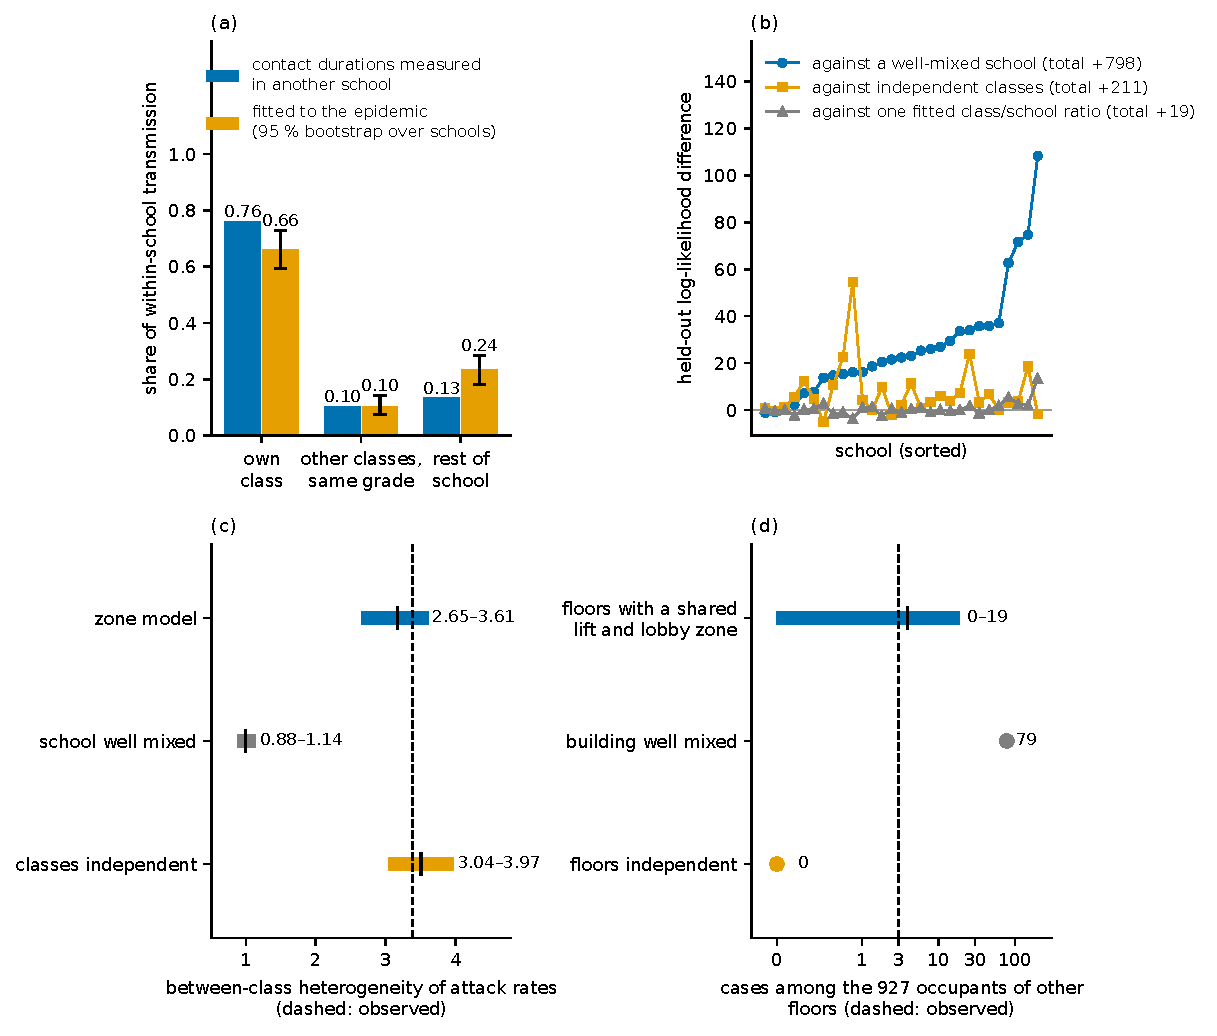
\includegraphics[width=\textwidth]{v2_zone_en}
  % generated by code/v2_figures.py (zone) from data/bsc_validation2/a4_zone_level/{matsumoto_primary.json, seoul_floors.json} and data/schools/lyon_mixing.json
  \caption{Zone level. (a)~Shares of within-school transmission by level: measured contact durations in a
  primary school in Lyon and shares fitted to the influenza epidemic in Matsumoto. (b)~Held-out
  log-likelihood of the zone model minus that of three competitors, by school. (c)~Heterogeneity of attack
  rates between classes: 95\,\% predictive interval of three models. (d)~Seoul call-centre building: cases
  among the occupants of the other floors predicted from the 11th floor; the bar is a prior-predictive
  interval over an assumed time in the shared lifts and lobby, not a measurement.}
  \label{s8b_evidence:fig:zone}
\end{figure}

\paragraph{Result: the structure, not the numbers.} (Model definitions and power: Section~\ref{appS_prot2:sec:zones}.)
Table~\ref{s8b_evidence:tab:zone} and Fig.~\ref{s8b_evidence:fig:zone} give the outcome, which the
re-check reproduced from data downloaded again, with full-data likelihoods equal to six digits. The zone model
predicts held-out schools far better than a well-mixed school ($+798$ units of log-likelihood, ahead in 27 of
29 schools) and than independent classes ($+211$). The share between classes of the same grade agrees to
two decimals (0.10). Exact agreement of the three shares is rejected (likelihood ratio 42.7): the measured
own-class share is larger than the fitted one, 0.76 against 0.66, and the fitted school-level share is almost
twice the measured one, 0.24 against 0.13. This comparison is confounded. The model has no household term,
whereas the source attributes 41\pct{} of the pupils' infections to households (51\pct{} to school, 8\pct{} to
the community); siblings attend the same school in different grades, so infections between siblings at home
appear as transmission across the school and inflate the fitted school-level share. The shortfall of the
measured school share is therefore probably overstated by this confounding; how much cannot be estimated from
the released table, which has no household identifier, and other unmodelled sources (the external hazard,
contact time as a proxy for transmission) act in directions that are not known. The source itself, with households and the community in its
model, estimated from the same data that transmission to classmates makes up about two-thirds of the
within-school reproduction number when a grade has a single class \citep{endo2021within}; the fitted own-class
share here, 0.66, is of that size. The fitted shares lie within the tolerance (0.103), but not securely: the bootstrap interval
of the distance reaches 0.168, 11\pct{} of resamples exceed the limit, and so does one of the sensitivity
analyses listed in the protocol (no winter break: 0.162). Among the models of the protocol the third tier
excludes only the well-mixed school; the interval of the generic two-level model, simulated afterwards by the
re-check (2.32 to 3.11), does not contain the observed 3.38, a small point in favour of the zone
model. The verdict of the rule, `right structure within tolerance, not exact', is therefore reported as a weak pass.
% src: Endo et al. 2021, Results and Discussion (Europe PMC PMC8609560, read 1 October 2026: school 51.1 %, household 41.3 %, community 7.7 % of student cases; classmates about two-thirds of the within-school reproduction number when a grade has one class); data/v2_numbers.json (zone.posthoc.schools_Z_ahead_of_H [27, 29]; zone.primary_other.LR_F_vs_Z 42.71, w_hat; zone.TV_boot_ci; zone.check.P_TV_gt_0.15 0.107; zone.sensitivity.no_break_switch.TV 0.162); code/bsc_validation2/a4_zone_level/POSTHOC_LOG.md (P4); data/v2_numbers.json (zone.check.disp_C: [2.32, 2.71, 3.11]); notes/VERIFICATION.md (Section 4.9, zone level, items 4, 5, 7; further point 4)

Two comparisons bound what the pass means. First, the generic two-level model with one fitted ratio is not
beaten: the zone model is ahead by 18.8 out of sample, with an interval that includes zero, and the generic
model fits the full data better by 13.6. What the measurement supplies is a ratio that the generic model has to
fit: about 62 implied by the Lyon shares in the Matsumoto class structure, against 37 fitted. Second, a
comparison added during the re-check asks whether measured mixing does better than a guess, in two runs that differ only in the lower
bound of $10^{-9}$ on the external hazard of the protocol. With that bound, a zone model with the round shares
0.7, 0.1 and 0.2 predicts held-out schools better than the measured shares by 19 units (3 to 38), and the
guess two-thirds, one-sixth, one-sixth by 8.9 ($-12.1$ to 34.5, not significant); without it, the guess 0.7, 0.1, 0.2 is better by 34 (11 to 66)
and 0.6, 0.2, 0.2 by 25 ($-17$ to 76). Guesses with 80\pct{} or more in the own class and equal thirds do worse
(all three significantly), and so, in point estimate only, does 0.5, 0.25, 0.25 (by 30, $-30$ to 83;
run without the bound). These guesses were chosen after the fitted shares were known. With that reservation, the measurement is not shown to matter beyond the statement that most
transmission is within the class. Had contact been counted as distinct pairs per day instead of duration, a
choice the protocol excluded in advance, the shares would have been 0.43, 0.14 and 0.43 and the tolerance
would have been missed (0.23). And at the ratio that the data favour, a world in which the generic model is
true earns the full verdict in about 38\pct{} of synthetic replicates (6 of 16), far above the 0 to 7.5\pct{}
obtained when the ratio is drawn at random.
% src: data/v2_numbers.json (zone.D_Z_minus_C; zone.posthoc: AIC, rho_fitted_C.full 36.6, rho_implied_by_Lyon_per_class_quantiles median 61.8; zone.check.hazard_bound."1e-09": D_N702 -19.1 [-37.8, -3.3], D_N2/3 -8.9 [-34.5, 12.1], D_N811 +18.6 (run with the bound); zone.check.D_Z_minus_N_.7_.1_.2: -34.5 [-66.3, -10.6]; zone.check.D_Z_minus_N_.6_.2_.2: -25.3 [-75.8, 17.0]; zone.check.D_Z_minus_N_.5_.25_.25: 29.6 [-29.5, 82.9] (run without the bound); zone.check.TV_naive.Lyon_distinctpairs 0.231); data/checks/zones.json: generic_ratio_model_at_fitted_ratio (6/16 at ratio 37), full_data_log_likelihood_advantage_of_constant_ratio_model (13.6); notes/VERIFICATION.md (Section 4.9, zone level, items 9, 7, 8)

The frequency-dependent normalisation of eq.~\eqref{M-s8b_evidence:eq:zone} fits better than a
density-dependent transfer of the measured contact times, by 37 units of log-likelihood on the full data, in a
sensitivity analysis that the re-check did not re-run. The source had already reported, from the same data,
that the within-school reproduction number hardly depends on class size or the number of classes, that is,
frequency-dependent mixing \citep{endo2021within}; the comparison here agrees with it and adds nothing
independent of it.
% src: data/v2_numbers.json (zone.sensitivity: base_full_data LR_F_vs_Z 42.7, density_dependent_transfer LR_F_vs_Z 116.5); Endo et al. 2021, Results (Europe PMC PMC8609560, read 1 October 2026: R_S "not significantly associated with n or m", "suggesting frequency-dependent mixing"); notes/VERIFICATION.md (Section 4.9, zone level, item 10: unverifiable)

\paragraph{A building by floor: inconclusive.}
The Seoul call-centre building had 94 cases among the 216 people on the 11th floor and 3 among the 927
occupants of the other floors \citep{park2020}. A zone model with one zone per floor and a shared zone of
lifts and lobby, its rate calibrated on the 11th floor alone, predicts a median of 4 cases elsewhere (interval
0--19); a well-mixed building would have had 79. The time spent in the shared zone is not measured, however:
it is a prior of 3 to 30 minutes a day, placed after a rough calculation on the observed counts, and with 30
to 120 minutes the same model would be inconsistent with the data. The check shows that a well-mixed building
is excluded, which needs no model, and nothing more. For the two wings of the 11th floor, and for the
statements of Section~\ref{M-s4_geometry:sec:hotspots} on early growth and on the concentration of risk in
high-efficiency zones, no outbreak with an independent measurement of mixing was found (a cruise ship, a
warship, the meat-processing plant, prisons and nursing homes were considered), and no test was run.
% src: data/v2_numbers.json (zone.seoul: pred_count_median 4, interval [0, 19], well_mixed_expected 78.7, obs_other 3, N_other 927); data/checks/zones.json: seoul_by_floor (30-120 min gives 7 to 81; notes/VERIFICATION.md, Section 4.9, zone level, item 11); code/bsc_validation2/a4_zone_level/PREREGISTRATION.md sections 3, 4

\subsection{All events with a stratum test}

\begin{figure}[tbp]
  \centering
  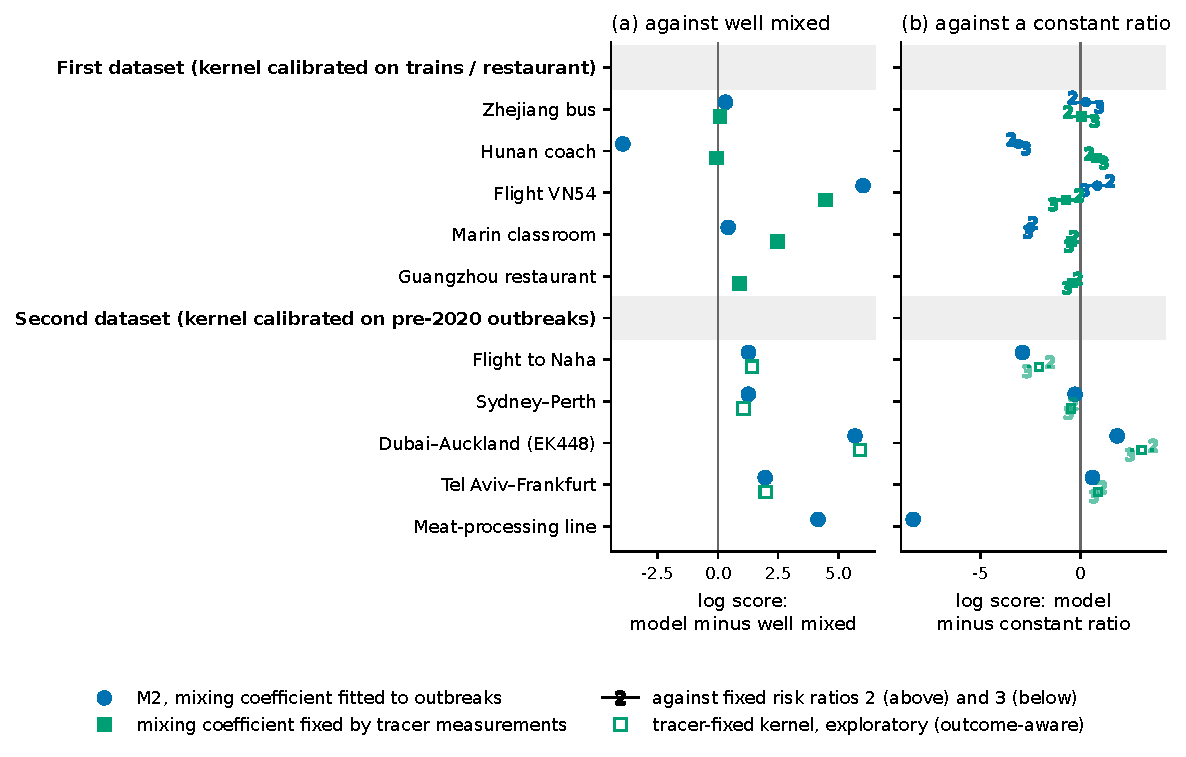
\includegraphics[width=\textwidth]{v2_summary_scores_en}
  % generated by code/v2_figures.py (summary_scores) from data/v2_numbers.json (first.per_event),
  % data/bsc_validation2/a1_more_outbreaks/10_corrected.json, data/bsc_validation2/a3_tracer_physics/04_evaluation.json and E2_ext_evaluation.json
  \caption{Every event with a stratum test, in both datasets: difference of log scores (a)~between the spatial
  kernel and the well-mixed model and (b)~between the spatial kernel and a constant near/far risk ratio.
  Positive values favour the kernel. Circles: $\Mtwo$ with the mixing coefficient fitted to outbreaks (first
  set: train cohort for vehicles, restaurant for the classroom; second dataset: the six pre-2020 events). In (b)
  the first dataset is compared with the fixed ratios 2 and 3 (digits; introduced after unblinding) and the second
  with the ratio calibrated on the same events as the kernel. Squares: the kernel with its coefficient taken
  from tracer measurements, against the ratios 2 and 3; open squares: its exploratory, outcome-aware application
  to four flights of the second dataset. The restaurant is a calibration event of the first test and has no
  circle; the processing line has no tracer measurement. The kernel is to the right of zero in (a) for all events
  but the coach, and scattered about zero in (b).}
  \label{s8_outbreaks:fig:summary}
\end{figure}

% supp_protocol2.tex -- Supplementary Section S10: protocols of the second outbreak test and of the further analyses; register of all tests.
% Paths in "% src:" comments are relative to the repository root.
% Numbers: data/v2_numbers.json and data/v2_tab_*.tex (code/v2_numbers.py).
\section{Protocols of the second outbreak test and of the further analyses; register of all tests}\label{appS_prot2:sec}

This section documents the four analyses of Section~\ref{M-s8_outbreaks:sec} of the main text other than the first
outbreak test: what was fixed in advance and the evidence for when; the decision rules and their
power; the data and what may be redistributed; and a register of every test of Section~\ref{M-s8_outbreaks:sec}, which separates what
was pre-specified from what was added afterwards, by the analysis itself or by its re-check. The four
protocols, their power addenda, freeze records and post-hoc logs are released with the code, under the file
names they were given (\texttt{PREREGISTRATION.md} and so on), as redacted copies (Section~\ref{appC_protocol:sec});
as in
Section~\ref{appC_protocol:sec}, they are called protocols here and their contents pre-specified. `The
re-check' of an analysis is its re-implementation with separately written code, within the same project and
on the same machine, as described in Section~\ref{M-s1_intro:sec}; where it corrected a result, the corrected result is the one reported.
Where the frozen protocol texts and logs speak of a `verifier', they mean this
same-project re-check, not an independent party, and by `the analyst' they mean the first analysis (both
passes were made by the author). The
frozen protocol texts call the four analyses avenues 1 to 4, and the first outbreak test with its dataset and the
later analyses rounds 1 and 2 (two successive sets of analyses); the article does not use these labels.

\subsection{What was frozen, and the evidence for when}\label{appS_prot2:sec:freeze}

\begin{table}[tbp]
  \centering\footnotesize
  \caption{The four protocols of the second outbreak test and of the further analyses. Times are British Summer Time on 1~October 2026, from the
  freeze records (self-reported) and from the modification times of the files. Hashes: number of files whose
  SHA-256 is stored in the freeze records; all were recomputed for this article on the unredacted originals
  and match.}
  \label{appS_prot2:tab:freeze}
  % src: data/v2_numbers.json (freeze) <- code/bsc_validation2/a*/PREREG_FREEZE.json, FIX_FREEZE.json, PREREG_FREEZE_2_before_unblinding.json, PREREG_EXT_FREEZE*.json; file times of the working tree
  \setlength{\tabcolsep}{4pt}
  \begin{tabular}{@{}>{\raggedright\arraybackslash}p{0.12\textwidth}>{\raggedright\arraybackslash}p{0.21\textwidth}c>{\raggedright\arraybackslash}p{0.24\textwidth}>{\raggedright\arraybackslash}p{0.24\textwidth}@{}}
    \toprule
    Analysis & Frozen & Hashes & First result that uses outcomes & Known beforehand \\
    \midrule
    Further outbreaks (Section~\ref{M-s8_outbreaks:sec:second}) &
      protocol 09:42:01; calibration and power 09:52:41 & 4 + 6 &
      held-out strata scored 09:53:08 &
      every count, including the held-out ones; the outcome of the first test \\
    Contact records (Section~\ref{M-s8b_evidence:sec:contacts}) &
      protocol 09:23:27; modified walks 10:34:24, before the confirmatory datasets & 8 + 26 &
      first dataset 09:24:00 (the run takes 19\,s); first confirmatory dataset 10:35:34 &
      raw counts per day and group labels; the published properties of such data; expectation of failure
      written down \\
    Tracer measurements (Section~\ref{M-s8b_evidence:sec:tracer}) &
      protocol 09:18:16; kernels, predictions and power 09:44:43 & 23 + 10 &
      evaluation 09:49:08 &
      the outbreak counts and the failures of the first test; the tracer sources had been opened \\
    \quad extension to four flights &
      protocol 10:24:56; predictions 10:26:01 & 7 + 4 &
      evaluation 10:26:09 &
      the near/far counts and the result of the second outbreak test: outcome-aware \\
    Zone level (Section~\ref{M-s8b_evidence:sec:zones}) &
      protocol 09:48:58 & 14 &
      schools 09:56:44 (run 09:49--09:56); floors 10:21:08 &
      total of cases; qualitative conclusion of the source; for the floors, the counts \\
    \bottomrule
  \end{tabular}
\end{table}

Table~\ref{appS_prot2:tab:freeze} gives the times. The limits are those of the first test
(Section~\ref{appC_protocol:sec:freeze}) and apply to all four analyses.
(i)~Every protocol is \emph{data-aware} and \emph{model-blind}. What was fixed in advance is the list of
events or datasets, the models, the split into calibration and hold-out, the metrics, the decision rule and
the list of sensitivity analyses, each with a power analysis; the data themselves had been read.
(ii)~The freezes are self-attested. The records are files on the author's machine, with matching hashes and
no external time stamp or version-control history; the hashes show that the files have not changed since, not
when they were written. In the outbreak analysis the record was itself rewritten when the power addendum was
added, and the clock times written into its post-hoc log are one to two hours ahead of the file times.
(iii)~Parts of the code were written after the freeze: in the outbreak analysis the modules that build the
events and run the comparison (the last one four seconds before the hold-out output), in the tracer analysis
the evaluation script. The intervals are short because each analysis was prepared and run in one or two continuous stretches of
work.
(iv)~In the outbreak analysis the constant-ratio model was coded as $p_j=1-\exp(-\varepsilon\varrho)$ in the near
zone, not as the $p_j=\varrho\,p_0$ of the protocol. With the form of the protocol the pooled
$\Delta_{\mathrm{C}}$ is $-7.19$ in the re-check's re-implementation, against $-9.20$; the outcome is the
same.
(v)~The extension of the tracer analysis to four flights was written, run and evaluated within 73 seconds,
with the outcomes known; its freeze is nominal, and it is reported as exploratory throughout.
% src: notes/VERIFICATION.md (Section 4.6, second outbreak test, item 1; Section 4.7, contact records, item 1; Section 4.8, tracer measurements, items 1, 13; Section 4.9, zone level, item 1); data/v2_numbers.json (out2.check.registered_form.all: deltaC -7.194; freeze: extension protocol 10:24:56, evaluation 10:26:09)

\subsection{Further outbreaks: rule, power, numerical correction}\label{appS_prot2:sec:outbreaks}

\begin{table}[tbp]
  \centering\footnotesize
  \caption{(a)~Decision rule of the second outbreak test, applied to $\Mtwo$ (and, in separate columns of the
  analysis, to $\Mone$ in closed form and to an exploratory variant with a well-mixed fraction). (b)~Probability
  of each criterion and of the full claim V1 when the data are generated by the model in the first column, at
  its calibrated posterior (200{,}000 replicates), as computed before any held-out stratum count was scored
  and, in brackets, after the numerical correction of the room kernel.}
  \label{appS_prot2:tab:rule}
  % src: code/bsc_validation2/a1_more_outbreaks/PREREGISTRATION.md section 7; code/bsc_validation2/a1_more_outbreaks/src/a1/pipeline.py (V5 if two or more failures; elif not B1: V4; elif mirror: V3; elif B2 and no failure: V1; else V2); data/v2_numbers.json (out2.power.registered, out2.power.corrected (M2: B1B2 0.926 - V1 0.762 = 0.164), out2.power.registered_air)
  \begin{tabular}{@{}l>{\raggedright\arraybackslash}p{0.40\textwidth}>{\raggedright\arraybackslash}p{0.46\textwidth}@{}}
    \toprule
    \multicolumn{3}{@{}l}{(a) \emph{Criteria and outcomes}} \\
    B1 & better than well mixed & $\Delta_0>0$ with one-sided $p<0.05$ under $\Mzero$ \\
    B2 & better than the constant ratio & $\Delta_{\mathrm{C}}>0$ with one-sided $p<0.05$ under the
         constant-ratio model; mirror: $\Delta_{\mathrm{C}}<0$ with $p<0.05$ under $\Mtwo$ \\
    B3 & adequacy & two-sided predictive $p\ge0.05$ for every held-out event \\
    \midrule
    V1 & B1, B2, B3, and power of (B1 and B2) at least 0.8 &
         `predicts held-out distance gradients better than both a well-mixed model and a constant near/far
         risk ratio' \\
    V2 & B1 and B3 with at most one failure; neither B2 nor its mirror &
         `better than well mixed; not distinguishable from a constant ratio' \\
    V3 & B1; mirror of B2 & `better than well mixed, but a constant ratio predicts better' \\
    V4 & B1 not met & `no out-of-sample support for the kernel' \\
    V5 & two or more failures of B3 & a list of the events reproduced and of those not \\
    \multicolumn{3}{@{}p{0.95\textwidth}@{}}{\emph{Not covered:} B1 and B2 met with exactly one B3 failure was given no
    outcome by the protocol (probability 0.16 if $\Mtwo$ is true); the code classes it with V2. The observed
    outcome, V5, does not depend on this.} \\
    \bottomrule
  \end{tabular}

  \medskip
  \begin{tabular}{@{}lcccc@{}}
    \toprule
    (b) Truth & B1 & B2 & B1 and B2 & V1 \\
    \midrule
    well mixed       & 0.007 (0.015) & 0.096 (0.169) & 0.005 (0.010) & 0.003 (0.008) \\
    constant ratio   & 0.652 (0.732) & 0.029 (0.052) & 0.028 (0.049) & 0.020 (0.039) \\
    $\Mtwo$          & 0.989 (0.982) & 0.961 (0.935) & 0.956 (0.926) & 0.784 (0.762) \\
    \midrule
    $\Mtwo$, four flights only & 0.980 & 0.822 & 0.821 & -- \\
    \bottomrule
  \end{tabular}
\end{table}

The rule of Table~\ref{appS_prot2:tab:rule} was written to remove the weakness found in the first test: a
constant-ratio world passes B1 with probability 0.65 to 0.73, so that B1 alone is no evidence for the
kernel, and passes B1 and B2 together with probability 0.03 to 0.05. The re-check recomputed the
power from 400{,}000 draws of its own (0.927, 0.048 and 0.010 for B1 and B2 together under the three truths;
0.822 for the four flights).
% src: data/v2_numbers.json (out2.power.check: all M2 P_B1B2 0.9268, CRR 0.0476, M0 0.0100; air M2 0.8222)

\paragraph{The numerical correction.}\label{appS_prot2:sec:numerics}
The propagator of the first test writes $P_t(y|x)$ on a rectangle with reflecting walls as a sum over cosine
modes. Its absolute error reaches about $10^{-10}$ of the largest exposure in an event, so that receivers
whose true exposure is smaller than that carry round-off noise of either sign. Replacements by the corrected
propagator occur for mixing coefficients up to about 2.5 to $16\sqmh$, in the cabins and in the rooms of the
second test alike. The posterior of
the room coefficient first computed (`mode $0.02\sqmh$, bimodal') came from two such noise values in the
likelihood of the ward inpatients; it was found by inspection of a diagnostic plot after the held-out events
had been scored. In the corrected code each one-dimensional propagator is a positive sum of image terms, and
the image value replaces the mode sum wherever the latter is below $10^{-8}$ of the event maximum; where both
are resolved, at coefficients at which a replacement occurs, they agree to about $10^{-4}$ or better
(largest relative difference $8.4\times10^{-5}$, in the ward inpatients). The primary analysis, the power and the secondary analyses were then
re-run unchanged (the analyses stored in \texttt{10\_corrected.json}); the 15 sensitivity variants were not,
and are reported with the kernel as first frozen. For the flights no reported
digit changes (their posterior lies above the affected range). For the rooms the posterior becomes $794\sqmh$
(302--4{,}390), the score of the processing line $-15.24$ instead of $-16.22$ and its predictive $p$
$1.4\times10^{-5}$ instead of $5\times10^{-6}$; the pooled scores are $+14.35$ and $-9.15$ instead of $+13.37$
and $-10.13$; and the outcome is V5 in both cases. Both versions are stored. The re-check confirmed
the defect and the correction with a third propagator, built by uniformisation and sharing no code with
either: it agrees with the image sum to $10^{-14}$ at small coefficients, while the mode sum returns
non-positive exposures at up to 32 of the 74 ward receivers. On the restaurant calibration of the first test
the same defect changes the log-likelihood by about $10^{-7}$ at most at every coefficient in the posterior range,
so that calibration is not affected. The hold-out predictions of the first test were affected in the
classroom, where the mode sum returns non-positive exposures at up to 11 of the 24 desks for coefficients of
$0.1\sqmh$ and below; they were re-run with the corrected propagator for this article
(Section~\ref{M-s8_outbreaks:sec:holdout}).
% src: data/bsc_validation2/a1_more_outbreaks/09_numerics_check.json (per event: last coefficient with frac_replaced > 0: 2.5 (F2, F3, F4, F6, P1), 6.3 (F1, W2), 15.8 (F5, F7, F8, W1); max_rel_diff_where_resolved at those coefficients up to 8.4e-5 (W2)); data/s8_first_test_exact.json (kernel.rows: spectral_min_rel down to -1.28e-10); code/checks/outbreaks2/t6_first_set_floor.json (restaurant: 1.1e-7)
% src: code/bsc_validation2/a1_more_outbreaks/POSTHOC_LOG.md (P5); data/v2_numbers.json (out2.pooled_registered.M2.all, out2.pooled_registered.P1: M2 logp -16.22, p 4.9e-6; out2.hold.P1.M2: logp -15.24, p 1.42e-5); notes/VERIFICATION.md (Section 4.6, second outbreak test, item 13: confirmed); data/s8_first_test_exact.json (kernel.rows: spectral_nonpositive up to 11 of 24)

\begin{table}[tbp]
  \centering\small
  \caption{Mixing coefficient preferred by each event of the second dataset taken alone (profile likelihood of the
  stratum counts given the total; interval where the log-likelihood is within 1.92 of its maximum; grid from
  $10^{-2}$ to $10^{4}\sqmh$), and gain in log-likelihood over the largest coefficient of the grid
  ($10^{4}\sqmh$), which in a cabin is close to, but not yet, the well-mixed model.}
  \label{appS_prot2:tab:Dprofiles}
  % generated: data/v2_tab_Dprofiles.tex (code/v2_numbers.py <- data/bsc_validation2/a1_more_outbreaks/10_corrected.json, preferred_D_corrected)
  \begin{tabular}{@{}llccc@{}}
    \toprule
    Event & Pathogen & $\Dair$ ($\mathrm{m^2\,h^{-1}}$) & Interval & Gain \\
    \midrule
    \tabinput{data/v2_tab_Dprofiles}
    \bottomrule
  \end{tabular}
\end{table}

\begin{figure}[tbp]
  \centering
  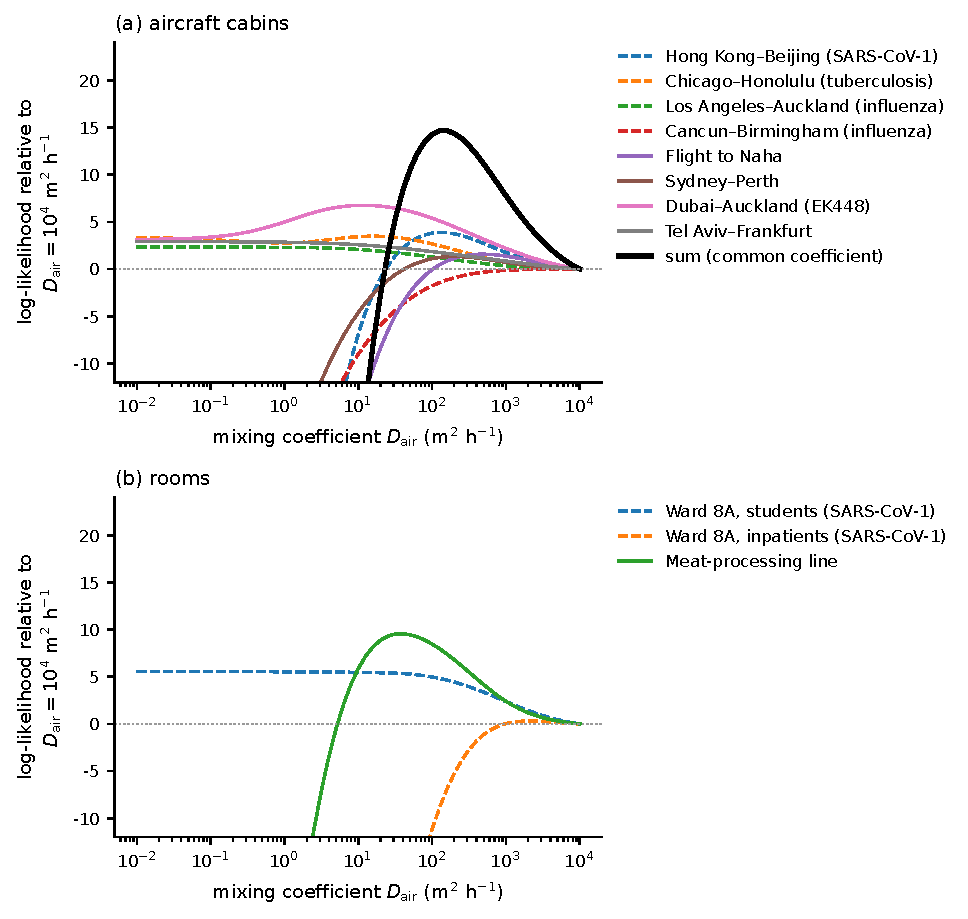
\includegraphics[width=\textwidth]{v2_D_profiles_en}
  % generated by code/v2_figures.py (D_profiles) from data/bsc_validation2/a1_more_outbreaks/10_corrected.json (preferred_D_corrected.*.curves)
  \caption{Log-likelihood of the mixing coefficient of $\Mtwo$ for each event of the second dataset taken alone,
  relative to the largest coefficient of the grid ($10^{4}\sqmh$). Solid: held-out events; dashed: calibration events. The thick line in (a)
  is the sum over the eight flights (common coefficient).}
  \label{appS_prot2:fig:Dprofiles}
\end{figure}

\subsection{Contact records: data and statistics}\label{appS_prot2:sec:contacts}

\begin{table}[tbp]
  \centering\footnotesize
  \setlength{\tabcolsep}{3.6pt}
  \caption{The six contact datasets (SocioPatterns, RFID proximity at 20\,s resolution) and four statistics of
  the test days, observed and under the homogeneous lattice walk calibrated on the training days. Role:
  development (dev.) or confirmatory (conf.) dataset for the modified walks. Days: training + test. Sites: size of the lattice fixed by the calibration. Exponent: of the number of contacts per
  20 minutes against the number of people present (not comparable for the primary school, where occupancy
  hardly varies; the conference has no groups).}
  \label{appS_prot2:tab:datasets}
  % generated: data/v2_tab_datasets.tex (code/v2_numbers.py <- data/bsc_validation2/a2_contact_mobility/{s1,s3a}_<dataset>.json)
  \begin{tabular}{@{}>{\raggedright\arraybackslash}p{0.19\textwidth}lccccccc@{}}
    \toprule
     & & & & & \multicolumn{4}{c}{observed / walk} \\
    \cmidrule(l){6-9}
    Setting & Role & People & Days & Sites & \shortstack{Partners\\per day} & \shortstack{Within-group\\share} &
      Burstiness & Exponent \\
    \midrule
    \tabinput{data/v2_tab_datasets}
    \bottomrule
  \end{tabular}
\end{table}

\begin{figure}[tbp]
  \centering
  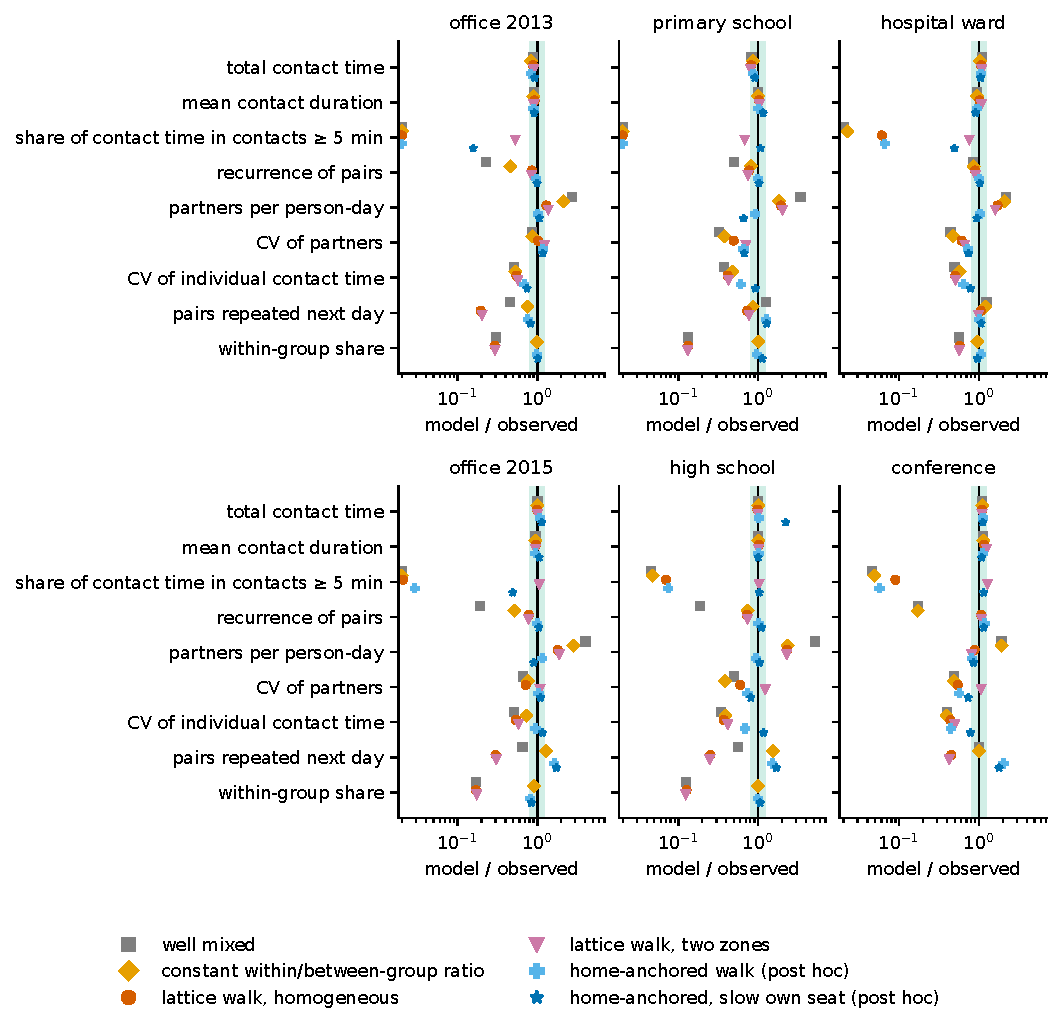
\includegraphics[width=\textwidth]{v2_contacts_structure_en}
  % generated by code/v2_figures.py (contacts_structure) from data/bsc_validation2/a2_contact_mobility/*.json (obs, models.*.stats)
  \caption{Contact statistics of the test days: value under each model divided by the observed value (shaded:
  tolerance 0.8 to 1.25; values below 0.02 are drawn at the left edge). The lattice walk matches what it was
  calibrated on, the total contact time and the mean duration, and misses long contacts, the number of
  partners, the differences between people, the repetition of pairs and the group structure. The anchored
  variants were developed on the first three datasets (top row) after that failure.}
  \label{appS_prot2:fig:structure}
\end{figure}

Table~\ref{appS_prot2:tab:datasets} lists the datasets. The first three were used to develop the modified
walks and the last three were not touched by any model or statistic until the modifications and their fitting
code had been frozen. Clock offsets, the removal of days with fewer than 1\pct{} of the records and the
definition of a person's presence (from the first to the last own contact of the day) are fixed in the frozen
loader. The seven families of statistics, with their tolerances, are: total contact time (ratio in 0.8--1.25);
mean contact duration and share of contact time in contacts of at least five minutes; burstiness of the gaps
between a person's contacts (absolute difference at most 0.10) and recurrence of pairs; mean and coefficient
of variation of the number of partners per person and day; coefficient of variation of individual contact
time; share of a day's pairs already in contact on the previous day; share of contact time within the recorded
groups. A family is passed if all its statistics are.
% src: code/bsc_validation2/a2_contact_mobility/PREREGISTRATION.md sections 2, 5; code/bsc_validation2/a2_contact_mobility/FIX_FREEZE.json
The power analysis was made on synthetic data before the freeze, with four replicates per combination of
generating model and candidate: a true or nesting model passed every family and the epidemic criterion in 20
of 20 replicates, and a wrong non-nested model reached the per-dataset criterion in none of 44. The
re-check qualified this in three ways: the 44 cases are not independent; the analysis covers the
base models only, and the modified walks fail on their own synthetic truth
(Section~\ref{M-s8b_evidence:sec:contacts}); and on real data the tolerance of the epidemic criterion is at the
level of the noise, since two runs of 4{,}000 epidemics on the same recorded network differ by up to 7\pct{} in
the secondary cases of the index case, against a tolerance of 10\pct. The rule is therefore adequate for the
failure of the lattice walk, whose errors are 25 to 72\pct{}, and weak for anything close to the tolerance.
% src: code/bsc_validation2/a2_contact_mobility/PREREGISTRATION.md section 7; code/bsc_validation2/a2_contact_mobility/POSTHOC_LOG.md item 1; data/checks/contacts.json: power (20/20, 0/44), noise_of_epidemic_criterion (4,000 runs, up to 7 %, tolerance 10 %), lattice_walk_errors_pct (25, 72); notes/VERIFICATION.md (Section 4.7, contact records, item 9: partially confirmed)

\subsection{Tracer measurements: rule and power}\label{appS_prot2:sec:tracer}

\begin{table}[tbp]
  \centering\footnotesize
  \caption{Tracer analysis. (a)~Decision rule over seven events (coach, bus, flight, trains, restaurant,
  classroom, call centre); D1: number of events rejected at the 5\,\% level; D2: pooled log score above that of
  $\Mzero$ with $p<0.05$; D3: above that of the constant ratios 2 and 3, each with $p<0.05$. (b)~Probability of
  each outcome when the data are generated by the model in the first column, computed after the kernels had
  been estimated and before any comparison with outbreak counts.}
  \label{appS_prot2:tab:tracerrule}
  % src: code/bsc_validation2/a3_tracer_physics/PREREGISTRATION.md section 6; data/v2_numbers.json (tr.power.truths.*.outcomes)
  \begin{tabular}{@{}l>{\raggedright\arraybackslash}p{0.82\textwidth}@{}}
    \toprule
    S1 & no D1 failure, D2 and D3: `with the kernel fixed by physical measurement the framework predicts the
         spatial patterns, and better than a generic gradient' \\
    S2 & no D1 failure, D2, not D3: `compatible with all events and better than well mixed; not shown to be
         better than a generic gradient' \\
    S3 & no D1 failure, not D2: `compatible, not discriminating' \\
    S4 & exactly one D1 failure: a sentence that names it \\
    S5 & two or more D1 failures: the hypothesis fails \\
    \bottomrule
  \end{tabular}

  \medskip
  \begin{tabular}{@{}lccccc@{}}
    \toprule
    (b) Truth & S1 & S2 & S3 & S4 & S5 \\
    \midrule
    tracer kernel     & 0.213 & 0.117 & 0.453 & 0.196 & 0.021 \\
    well mixed        & 0.009 & 0.004 & 0.488 & 0.401 & 0.099 \\
    constant ratio 2  & 0.017 & 0.204 & 0.112 & 0.455 & 0.211 \\
    constant ratio 3  & 0.000 & 0.022 & 0.002 & 0.204 & 0.773 \\
    \bottomrule
  \end{tabular}
\end{table}

The rule (Table~\ref{appS_prot2:tab:tracerrule}) is safe against a false claim and weak at confirming a true
one: if the tracer kernel were true it would earn the full claim S1 with probability 0.21 only, because on the
coach and the bus it predicts almost what the well-mixed model predicts. The outcome obtained, S4, has
probability 0.20 under the kernel, 0.40 if outbreaks are well mixed and 0.46 or 0.20 under a constant ratio of
2 or 3, so that it does not discriminate. Every model fails on the train table, and the rule counts this as a
failure of the kernel without asking whether a competitor passes. For the restaurant the rule fails the kernel
only if it is rejected at every count from two to five cases, which is lenient; the main text reports the
result at each count.
% src: data/v2_numbers.json (tr.power.truths: P S1 0.213, S4 0.196; M0 S4 0.401; CRR2 S4 0.455; CRR3 S4 0.204); code/bsc_validation2/a3_tracer_physics/POSTHOC_LOG.md (P7); notes/VERIFICATION.md (Section 4.8, tracer measurements, item 14)
Two departures from the protocol were forced by the data and are logged: the forward cabin has unmasked
breathing releases at three seats, not four, so that the flight uses two measured kernels in place of three;
and the minibus of the Hunan outbreak has 15 passengers with a simulated tracer value, not the 17 of the first
test. A full re-run of the stored analysis into a separate directory
reproduced every result file without a difference; the re-check then re-derived the coefficients
with its own solver (identical grid optima) and re-typed the tracer values from the sources.
% src: code/bsc_validation2/a3_tracer_physics/POSTHOC_LOG.md (P1, P2, P8); notes/VERIFICATION.md (Section 4.8, tracer measurements, items 2, 3: confirmed)

\subsection{Zone level: models and power}\label{appS_prot2:sec:zones}

A susceptible pupil of class $c$ has onset on day $t$ with probability $1-\exp(-\lambda_c(t))$,
$\lambda_c(t)=\beta\,x_c(t)+\alpha_0+\alpha_1P_{\mathrm{city}}(t)$, where $P_A(t)$ is the kernel-weighted
number of earlier onsets in the set $A$ per pupil of $A$ and the last term is the same quantity for the other
schools of the city. The kernel is a gamma density with mean 1.7 and standard deviation 1.0 days on daily bins,
as in \citet{endo2021within}, who chose it to give the mean serial interval of 2.2 days of influenza A(H3N2)
\citep{vink2014serial}. The three sets are exclusive: for a pupil of class $c$, $P_{\mathrm{class}}$ counts the
other pupils of the class (denominator $n_c-1$), $P_{\mathrm{grade}}$ the pupils of the other classes of the
grade and $P_{\mathrm{school}}$ the pupils of the other grades. The zone model has
$x_c=0.762\,P_{\mathrm{class}}+0.104\,P_{\mathrm{grade}}+0.134\,P_{\mathrm{school}}$, with the shares measured
in Lyon; the well-mixed school has $x_c=P_{\mathrm{whole\ school}}$; independent classes have
$x_c=P_{\mathrm{class}}$; the generic model has one fitted ratio $\varrho$ of own-class to rest-of-school risk;
and the ceiling has three free shares. Within-school terms are switched off during the winter break.
In the 36 grades that have a single class (453 pupils) the grade term is set to zero and not redistributed, so
that the shares of the zone model do not sum to one there; this was fixed in the protocol and its effect was
not assessed. The table holds the 2{,}548 pupils with an episode reported in the prospective survey of the
source (96\pct{} of the cases known to the schools) and the 8{,}375 who reported none in a later survey,
10{,}923 or 83\pct{} of the 13{,}217 enrolled; the missing pupils are mostly non-cases, so the denominators of
the classes are incomplete. The source excluded three small schools (71 pupils) from its own analysis; they
are kept here. The model has no household term, although the source attributes 41\pct{} of the pupils'
infections to households (Section~\ref{M-s8b_evidence:sec:zones}).
% src: code/bsc_validation2/a4_zone_level/PREREGISTRATION.md section 2.3; code/bsc_validation2/a4_zone_level/src/zonecore.py (features: Pc = Kc/(n-1), Pg = (Kg-Kc)/(ng-n), Ps = (Ks-Kg)/(ns-ng)); data/checks/zones.json: single_class_grades (36 grades, 453 pupils), respondents_share_of_enrolled_pct (82, as recorded; the 83 % of the text is 10,923/13,217 from the source, below) (notes/VERIFICATION.md, Section 4.9, zone level, further points 6, 7); Endo et al. 2021, Materials and Methods (Europe PMC PMC8609560, read 1 October 2026: 13,217 enrolled; 2,548 episodes, 96 % of the cases recognised by the schools; 8,375 without influenza in the retrospective survey; 10,923 combined; 71 pupils of 3 schools excluded; gamma kernel mean 1.7, SD 1.0, mean serial interval 2.2 d)
Power was computed before the freeze on synthetic epidemics on the real class structure (40 replicates per
truth, two strengths of the school signal). The verdict of the rule was earned in 100\pct{} and 80\pct{} of
replicates when the zone model is true, in none when the school is well mixed or the classes independent, in
7.5\pct{} and 0\pct{} under the generic model with a ratio drawn log-uniformly between 1 and 1{,}000, and in 2.5
and 5\pct{} under random shares. In the re-check the generic model turned out to be a more dangerous
competitor than these averages suggest: with its ratio set to the fitted value, about 37, it earns the verdict
in 6 of 16 replicates. The tolerance of 0.15 is a judgement, two to three times the sampling noise under a
true zone model; held-out differences depend slightly on a lower bound of $10^{-9}$ on the external hazard,
which is active in one fold (Table~\ref{s8b_evidence:tab:zone}).
% src: data/v2_numbers.json (zone.power); data/checks/zones.json: generic_ratio_model_at_fitted_ratio (ratio 37, 6/16); notes/VERIFICATION.md (Section 4.9, zone level, items 13, 7, 3)

\subsection{Register of tests}\label{appS_prot2:sec:register}

Table~\ref{appS_prot2:tab:register} lists every test of Section~\ref{M-s8_outbreaks:sec} of the main text, and the secondary and sensitivity
analyses of their protocols that are reported there and in Sections~\ref{appS_first:sec}--\ref{appS_prot2:sec},
with their status and their outcome after the re-checks. `Protocol' means that the test and its criterion were fixed before any model was run on
the data concerned; `listed' that the analysis is on the list of secondary or sensitivity analyses of a
protocol, which may never upgrade a primary outcome; `after' that it was added after results were known, by
the analysis or, where marked, by its re-check.

{\footnotesize
\setlength{\tabcolsep}{3pt}
\setlength{\LTcapwidth}{\textwidth}
\begin{longtable}{@{}>{\raggedright}p{4.6cm}>{\raggedright}p{1.5cm}>{\raggedright\arraybackslash}p{9.4cm}@{}}
\caption{Register of the tests of Section~\ref{M-s8_outbreaks:sec} of the main text and Sections~\ref{appS_first:sec}--\ref{appS_prot2:sec}.}
\label{appS_prot2:tab:register}\\
% src: default-parameter row: data/s8_default_level.json (expected_infections_bound 0.1021, 0.1570; beta_needed_per_day 16.34, 13.61 / 11.99)
% src: each row summarises Section 7 of the main text and Sections S7 to S9, where its numbers carry their own src comments; M1 row: data/v2_numbers.json (out2.pooled.M1.all: delta0 15.446, deltaC -8.055, p_mirror 1.5e-5; out2.pooled.M1.air: deltaC -4.634; out2.pooled.M1.decision); attainable totals: data/bsc_validation/02b_m1_exact.json, code/bsc_validation/POSTHOC_LOG.md (P4); zone rows: data/v2_numbers.json (zone.D_Z_minus_C; zone.check.hazard_bound."1e-09".D_N702); status: the four protocols and post-hoc logs; added rows: data/v2_numbers.json (out2.sec.train_kernel.rooms, out2.sec.loo_air, out2.sec.loo_room, out2.sec.seat, out2.sec.rho2.4, out2.pooled.M3.all, out2.pooled.M3.decision, out2.variants.summary, out2.rr_pooled."without P1", out2.check.bins."5 bins {0},{1},{2},{3-5},{6+}".air.deltaC -0.777, tr.power.pattern); data/s8_first_test_exact.json (primary.pooled.M2, loo_room)
\toprule
Test & Status & Outcome after the re-check \\
\midrule
\endfirsthead
\toprule
Test & Status & Outcome after the re-check \\
\midrule
\endhead
\bottomrule
\endfoot
\multicolumn{3}{@{}l}{\emph{First outbreak test (Section~\ref{M-s8_outbreaks:sec:holdout} of the main text and Sections~\ref{s8_outbreaks:sec:calibration}--\ref{s8_outbreaks:sec:outcomedetail})}} \\
Flight VN54, near/far split & protocol & pass ($\Mtwo$ $p=0.61$, $\Mzero$ $p=0.0008$); 20 passengers; a constant ratio of 2 to 3 also passes \\
Classroom, front/back split & protocol & not a real prediction: rejected at the calibrated value ($p=0.0009$); $p=0.068$ over the posterior \\
Bus, zone split & protocol & compatible ($p=0.38$), non-discriminating \\
Coach, rear/front split & protocol & fail ($p=0.007$) \\
Call centre, desk-scale clustering & protocol (quadrature after, check) & fail (0.007 to 0.013 by quadrature; 0.013 to 0.024 with the prior extended to $10^{6}\sqmh$; with the re-check's mode-sum propagator; its round-off acts only through the outbreak-size weights, and with zero weight at or below $0.1\sqmh$ the second value would be 0.015; the 40-draw estimate of the protocol had Monte Carlo error large enough to read as borderline) \\
Pooled test against $\Mzero$ & protocol & weak pass ($+2.83$, $p=2.5\times10^{-4}$, after the numerical correction of the classroom; $+3.87$ before), resting on the flight; constant ratios of 2 to 3 score higher (after, check) \\
Classroom with the round-off-safe propagator & after & $p=0.068$ instead of 0.11; outcome W4 unchanged \\
Totals attainable by $\Mone$ & protocol (rule P4 after) & mean number of cases below the observed one on bus, flight and classroom; observed total reached with probability 0.0002, 0.025 and 0.081, so unattainable under rule P4 on the bus only \\
Level checks and negative controls & protocol & met, with almost no power \\
Common coefficient, four vehicle events & after & rejected (approximate $p=0.023$, LR 9.52); for the two rooms not rejected (approximate $p=0.080$) \\
Default parameters of Sections~\ref{M-s2_model:sec}--\ref{M-s6_scenes:sec} against the bus and the choir & after & expected infections at most 0.10 and 0.16 against 23 and 52 (32 confirmed) cases; reached only for $\beta$ of about 16 and 14 (12)$\perday$ \\
\addlinespace
\multicolumn{3}{@{}l}{\emph{Second outbreak test (Section~\ref{M-s8_outbreaks:sec:second})}} \\
B1: $\Mtwo$ against $\Mzero$, five held-out events & protocol & pass ($+14.35$) \\
B2: $\Mtwo$ against the constant ratio, pooled & protocol & fail ($-9.15$), nine-tenths from the processing line, whose near zone was chosen by the source on the same data \\
B2 on the four flights & protocol & inconclusive ($-0.77$; power 0.82) \\
B3: adequacy of $\Mtwo$ & protocol & fail on 2 of 5 events; outcome V5 \\
$\Mone$ in closed form & protocol & V5, as $\Mtwo$; by the protocol a pass of the closed form, which overstates the reach of $\Mone$, does not bear on $\Mone$: against $\Mzero$ pass ($+15.45$); against the constant ratio pooled $-8.06$ (mirror $p=1.5\times10^{-5}$), on the flights $-4.63$; fails on 3 of 5 events \\
Train kernel applied to eight flights & listed & fail: four flights rejected \\
Exchange of calibration and hold-out & listed & weak pass on flights ($+3.58$, $p=0.004$); fail in the ward \\
Train kernel applied to the rooms & listed & rejected on the ward inpatients ($p=2\times10^{-5}$) and the processing line ($p=4\times10^{-4}$) \\
Leave one event out within each class & listed & flights not separated ($\Delta_{\mathrm{C}}=-0.06$; $p=0.046$ under the constant ratio, mirror $p=0.044$ under $\Mtwo$: improbable under either); rooms no better than well mixed, constant ratio better ($-14.0$) \\
Seat-level log score, three held-out flights & listed & constant ratio $-76.4$, $\Mtwo$ $-78.6$, well mixed $-83.5$ \\
Published ratio 2.4 in place of the calibrated one & listed & flights $+1.18$ ($p=0.028$); pooled $-4.44$ (mirror $p=0.002$; room kernel as first frozen) \\
Two-scale variant ($\Mtwo$ plus a well-mixed fraction) & protocol, exploratory & V3: $+17.5$ against well mixed, $-5.95$ against the constant ratio \\
Common coefficient within a class & listed & rejected (approximate $p$: rooms $1.6\times10^{-4}$, flights $0.034$) \\
Fifteen sensitivity variants & listed & V5 in 12, V3 in 3 (kernel as first frozen); on flights $\Delta_{\mathrm{C}}$ from $-3.42$ (constant ratio significantly better in three) to $+1.21$ ($\Mtwo$ significantly better in one) \\
Near/far risk ratios & listed & description: 3.98 (2.32--6.82; random effects); no gradient for influenza \\
Near/far ratio without the processing line & after & 3.30 (1.99--5.45) \\
Numerical correction of the room kernel & after & outcome unchanged \\
Other near zones and strata; ratio in the form of the protocol & after, check & $\Delta_{\mathrm{C}}$ on flights from $-0.78$ to $+7.8$ in these specifications; with the listed variants the sign is not determined \\
Exponential kernel & after, check & as good as $\Mtwo$ on flights, better on the processing line \\
\addlinespace
\multicolumn{3}{@{}l}{\emph{Contact records (Section~\ref{M-s8b_evidence:sec:contacts})}} \\
Lattice walk, structure and epidemic outcomes, six datasets & protocol & fail (A0) on all six \\
Walk against models without space & protocol & adds nothing; a static network of pair rates does better (after, check) \\
Modified walks on three confirmatory datasets & protocol (second freeze) & formally A0; uninformative, since the fit does not recover its own truth (after, check) \\
Error sizes of the modified walks & after & description only \\
Density scaling of contacts & listed & walk: exponent about 2; data below 1 in four of five settings \\
Power of the rule & protocol & adequate for the walk, weak near the tolerance \\
\addlinespace
\multicolumn{3}{@{}l}{\emph{Tracer measurements (Section~\ref{M-s8b_evidence:sec:tracer})}} \\
Coach & protocol & not rejected; non-discriminating \\
Call centre & protocol & not rejected; non-discriminating; wrong sign of clustering \\
Bus & protocol & inconclusive \\
Classroom & protocol & weak pass; constant ratios do as well \\
Flight VN54 & protocol & not reproduced (formal $p=0.14$; rejected in four of six listed variants) \\
Restaurant & protocol & not reproduced at the reported count \\
Trains & protocol & fail; every model fails \\
Pooled rule & protocol & S4 as computed, S5 on the defensible reading of the flight; not better than constant ratios \\
Probability of the pooled pattern under each truth & after, check & 0.23 under the tracer kernel, 0.84 and 1.00 under ratios 2 and 3 \\
Measured against fitted coefficients & listed & vehicle values 4.5 to about 50 times the first test's vehicle value; second-test aircraft value inside the cabin range, which does not make it a measurement of air mixing \\
Four further flights & after & exploratory, outcome-aware: weak \\
\addlinespace
\multicolumn{3}{@{}l}{\emph{Zone level (Section~\ref{M-s8b_evidence:sec:zones})}} \\
Tier 1: against well-mixed school and independent classes & protocol & pass \\
Tier 2a: equality of shares & protocol & fail \\
Tier 2b: tolerance; tier 3: dispersion & protocol & weak pass \\
Against a generic model with one fitted ratio & protocol (not decisional) & not beaten: zone model ahead by 18.8 ($-8.8$ to 54.0) out of sample, generic model better by 13.6 on the full data \\
Against guessed shares & after, check & guess 0.7/0.1/0.2 better by 19 (3 to 38); guesses chosen after the fitted shares were known; school-level share confounded by households \\
Frequency- against density-dependent transfer & listed & frequency-dependent fits better; not re-run by the check \\
Building by floor & protocol (low power, not blind) & inconclusive \\
Wings of one floor; early growth; hotspot maps & -- & not run: no independent measurement of mixing found \\
\end{longtable}
}

\subsection{Data, licences and what is redistributed}\label{appS_prot2:sec:data}

\emph{Outbreaks.} The seat maps and stratum counts of the eleven events were transcribed by eye from the
published figures and tables into the code and are released as tables, with the reference and the table or
figure of origin of every number (\texttt{data/outbreaks2/}). Copies of the source texts and figures are not
redistributed. \emph{Contact records.} The SocioPatterns files are distributed by their authors under
Creative Commons licences, some of which exclude commercial use; they are not redistributed here. A script
downloads them from the source and checks their SHA-256 against the values recorded when the protocol was
frozen. \emph{Tracer measurements.} The cabin measurements are published on figshare under CC~BY~4.0
\citep{kinahan2021aerosol}; the released tables are derived from those workbooks. The values for the coach and
the carriage were read or digitised from the supplementary figures of the sources and are released as tables
of numbers. \emph{Schools.} The anonymised pupil-level data of \citet{endo2021within} are published by their
authors under the MIT licence; the release contains a tabular copy, with that licence, and the script that
produced it from the original file.
% src: code/bsc_validation2/a2_contact_mobility/data/raw_SHA256.txt; data/tracer/SOURCES.md; code/bsc_validation2/a4_zone_level/PREREGISTRATION.md section 2.1 (MIT licence, commit 658abfe)

% supp_verification.tex -- Supplementary Section S11: numerical verification of the theorems and of the simulator;
% the re-checks of the analyses; reproducibility.
% Every number carries a "% src:" comment; paths are relative to the repository root.
% Numbers recomputed for this section: code/appA_numerics_checks.py
%   -> data/appA_numerics_checks.json (keys derived / adversarial / simulator).
\section{Verification of the theorems, the simulator and the analyses}\label{appA_numerics:sec}

The statements of Sections~\ref{M-s3_r0:sec} and~\ref{M-s4_geometry:sec} of the main text are proved in
Sections~\ref{appS_r0:sec} and~\ref{appS_geometry:sec}. This section records
the numerical tests that were run in addition, as a guard against errors in the proofs and in the code, and
the tests of the stochastic simulator used in Sections~\ref{M-s5_pair:sec} and~\ref{M-s6_scenes:sec}. Most
tests were carried out twice, by two sets of programs: the programs that produced the results of the article,
and a second set written separately for checking (the directories named \texttt{verify} in the repository),
which was also used to search for counter-examples. The second set does not call the first, except that the
schedule test of Section~\ref{s7_interventions:sec:time} and a timing benchmark run the production simulator;
other exceptions are stated. Monte Carlo uncertainties are standard
errors unless a 95\,\% interval is given in brackets.

\subsection{Scope of the re-checks}\label{appA_numerics:sec:scope}

Each strand of this work was re-checked with separately written code, within the same project and on the same
machine (Section~\ref{M-s1_intro:sec} of the main text). The re-check re-derived the proofs, re-implemented the
computations, including a second exact simulator, retyped the outbreak counts from the sources and searched for
counter-examples. Its core re-implementations were written separately; where it re-ran the analyses, compared
kernels or added comparisons, it reused modules of the analyses (data loaders of the contact and tracer analyses,
event geometries, the transcribed seat maps, the simulator for timing benchmarks and schedules). It was not carried
out by anyone independent of the project. The re-checks of the outbreak dataset and of the five tests are described
where their results are reported (Sections~\ref{appB_dataset:sec}--\ref{appS_prot2:sec}); this section describes
those of the theorems and of the simulator.
% src: notes/VERIFICATION.md (Section 4.1, theory, Section 4.2, simulations); notes/VERIFICATION.md (Section 4.4, outbreak dataset); notes/VERIFICATION.md (Section 4.5, first outbreak test); notes/VERIFICATION.md (Section 4.6, second outbreak test, Section 4.7, contact records, Section 4.8, tracer measurements, Section 4.9, zone level)

\subsection{Random-instance tests of the theorems}\label{appA_numerics:sec:theorems}

The tests of Table~\ref{appA_numerics:tab:theorems} use random instances drawn with a fixed seed and without
any tuning: connected lattices of $3$--$8$ by $3$--$8$ cells with a random fraction of the cells (up to about $30\,\%$)
removed, and
four families of movement generators, namely symmetric rates built from log-normal cell mobilities,
the departure-site rule (reversible with a non-uniform stationary distribution), non-reversible rates
(independent log-normal rates in the two directions of every edge), and dense irreducible generators of order
$3$--$11$ that are not lattices. The efficiency $q$ is log-normal, zoned with two to four levels, uniform with
about $30\,\%$ of zeros, or uniform on $[0.5,2]$; $\beta\in[0.02,3]\perday$ and $\gamma\in[0.05,2]\perday$.
% src: code/bsc_theory/scripts/verify_theorems.py (functions random_lattice, random_q, random_instance)
All computations are in double precision with dense eigen-solvers; the whole table takes 38\,s.
% src: data/bsc_theory/verify_theorems.json: runtime_s = 37.6
Figure~\ref{appA_numerics:fig:checks} shows the instances of the threshold and of the bounds tests.

\begin{table}[tbp]
\centering
\caption{Random-instance tests of the statements of Sections~\ref{M-s3_r0:sec} and~\ref{M-s4_geometry:sec}.
Deviations are relative unless stated; a `violation' is the amount by which an inequality fails
(positive values of the order of $10^{-14}$ are rounding errors of double precision).}
\label{appA_numerics:tab:theorems}
\footnotesize
\begin{tabular}{@{}>{\raggedright\arraybackslash}p{2.9cm}p{6.0cm}p{6.2cm}@{}}
\toprule
Statement & Test & Worst case over all instances\\
\midrule
Theorem~\ref{M-s3_r0:thm:ngm}(b) &
 $\bigl|\sabs(\gen+\Fm/\Rz-\gamma\Id)\bigr|$; 400 instances (103 symmetric, 119 departure-site, 96
 non-reversible, 82 dense) & $1.3\times10^{-14}$\\
% src: data/bsc_theory/verify_theorems.json: T1 (n_instances, kinds, max_abs_root_residual)
\addlinespace[3pt]
Theorem~\ref{M-s3_r0:thm:ngm}(c) &
 sign of $\Rz-1$ against sign of $\lamone$; $\lamone$ after replacing $\beta$ by $\beta/\Rz$; same 400
 instances & 0 sign failures; $|\lamone|\le1.3\times10^{-14}$\\
% src: data/bsc_theory/verify_theorems.json: T1 (sign_failures, max_abs_lambda_at_threshold)
\addlinespace[3pt]
Theorem~\ref{M-s3_r0:thm:ngm}(a) &
 $\Vm^{-1}$ against Gauss--Laguerre quadrature of $\int_0^\infty\e^{-\gamma t}\e^{\gen t}\,\dd t$ (one
 instance, 18 cells); Monte Carlo sojourn times of one infective, $4\times10^{6}$ infectious periods on a
 $3\times4$ lattice & $3.1\times10^{-6}$; largest $|z|=1.57$, root-mean-square $z=1.05$ over the 12 cells\\
% src: data/bsc_theory/verify_theorems.json: T1d_laplace_rel_err, T1e_mc (nrep, max_abs_z, rms_z)
\addlinespace[3pt]
Theorem~\ref{s3_r0:thm:rayleigh}, Corollary~\ref{s3_r0:cor:modal} &
 Rayleigh value against $\srad(\ngm)$; largest diagonal modal term against $\Rz$; monotonicity of the
 truncated modal formula; 150 symmetric and 100 departure-site instances &
 $8.0\times10^{-15}$ and $1.3\times10^{-14}$; diagonal term never above $\Rz$ (closest: $0.04\,\%$ below);
 0 monotonicity failures\\
% src: data/bsc_theory/verify_theorems.json: T1f (max_rel_rayleigh_err, max_rel_modal_minus_R0 = -3.96e-4,
%      ritz_monotone_failures), T1f_departure
\addlinespace[3pt]
Theorem~\ref{M-s3_r0:thm:bounds} &
 both bounds on $\Rz$ and on $\lamone$; 2{,}000 instances &
 violation $\le4.0\times10^{-14}$; for non-constant $q$ the gaps to the lower and upper bound are at least
 $1.1\times10^{-6}$ and $1.2\times10^{-3}$; constant $q$: $9.5\times10^{-15}$\\
% src: data/bsc_theory/verify_theorems.json: T2 (max_viol_lower 2.3e-15, max_viol_upper 4.0e-14,
%      min_gap_lower, min_gap_upper, const_q_rel_err)
\addlinespace[3pt]
Theorem~\ref{M-s3_r0:thm:mobility} &
 $\Rz(\Dz)$ at 41 values of $\Dz$ from $10^{-4}$ to $10^{4}$, limits at $\Dz=10^{\pm9}$, convexity of
 $\lamone(\Dz)$; 300 instances &
 strictly decreasing in every instance with non-constant $q$; largest increase in the other instances
 $2.7\times10^{-12}$; limits to $3.8\times10^{-6}$ and $2.6\times10^{-7}$; convexity violation
 $1.3\times10^{-15}$\\
% src: data/bsc_theory/verify_theorems.json: T3 (max_rel_increase, strict_failures = 0,
%      limit_inf_rel_err, limit_zero_rel_err, convex_monotone_violation); grid: verify_theorems.py, Dgrid
\addlinespace[3pt]
Proposition~\ref{M-s3_r0:prop:expansions} &
 ratio of the errors of each expansion at two values of $\Dz$ a factor 10 apart (100 for a second-order
 remainder) & median 99.9 (fast mixing, 227 instances) and 99.5 (slow mixing, 299 instances)\\
% src: data/bsc_theory/verify_theorems.json: T3 (largeD_ratio_median, smallD_ratio_median);
%      instance counts: data/bsc_theory/verify_theorems.log
\addlinespace[3pt]
Proposition~\ref{M-s3_r0:prop:zone} &
 878 random zones in 300 instances of all four families & no violation\\
% src: data/bsc_theory/verify_theorems.json: T3p (zone_trials, max_rel_violation_zone = 0.0)
\addlinespace[3pt]
Theorem~\ref{M-s3_r0:thm:edges} &
 900 increases of one edge rate by a factor 1--20, symmetric rates &
 largest increase of $\Rz$: $7.3\times10^{-16}$\\
% src: data/bsc_theory/verify_theorems.json: T3p (edge_trials, max_rel_increase_edge)
\addlinespace[3pt]
Theorem~\ref{M-s4_geometry:thm:closed}, Proposition~\ref{M-s3_r0:prop:kernel}(ii) &
 uniform $q$: 500 instances, square rooms of side 3 to 40, and 300 instances with random contact kernels &
 $8.3\times10^{-15}$; $\Rz=3.571429$ for every side; kernels: $5.8\times10^{-15}$, no violation of
 $\beta\qmin/\gamma\le\Rz\le\beta\qmax/\gamma$\\
% src: data/bsc_theory/verify_theorems.json: T4a_uniform_q_rel_err, T4a_size_scan, remarks_kernel
\addlinespace[3pt]
Theorem~\ref{M-s4_geometry:thm:leaky} &
 400 instances with random door cells and exit rates; corridors of 3 to 100 cells with absorbing ends &
 part (3): $2.1\times10^{-14}$; parts (2) and (4): violation $\le1.9\times10^{-15}$; absorbing limit (exit
 rate $10^{9}$): $1.3\times10^{-6}$; corridor formula: absolute error below $10^{-15}$\\
% src: data/bsc_theory/verify_theorems.json: T4b (uniform_q_rel_err, mu_upper_violation = 0,
%      mu_monotone_violation = 0, absorbing_limit_err, het_lower_violation = 0, het_upper_violation), T4d_1d;
%      corridor: data/appA_numerics_checks.json: derived/theorems/corridor_max_abs_err
\addlinespace[3pt]
Theorem~\ref{M-s4_geometry:thm:hotspots} &
 200 instances: long-time profile against $\uvec$; iterated generations against $\wvec$; $\sum_xe_x$;
 elasticity against central finite differences; reversible formula &
 $5.9\times10^{-14}$; $4.5\times10^{-14}$; $|\sum_xe_x-1|\le4.4\times10^{-16}$; $3.9\times10^{-5}$;
 $2.5\times10^{-14}$\\
% src: data/bsc_theory/verify_theorems.json: T5 (early_profile_err, generation_profile_err,
%      elasticity_sum_err, elasticity_fd_err, symmetric_qx2_err)
\bottomrule
\end{tabular}
\end{table}

\begin{figure}[tbp]
\centering
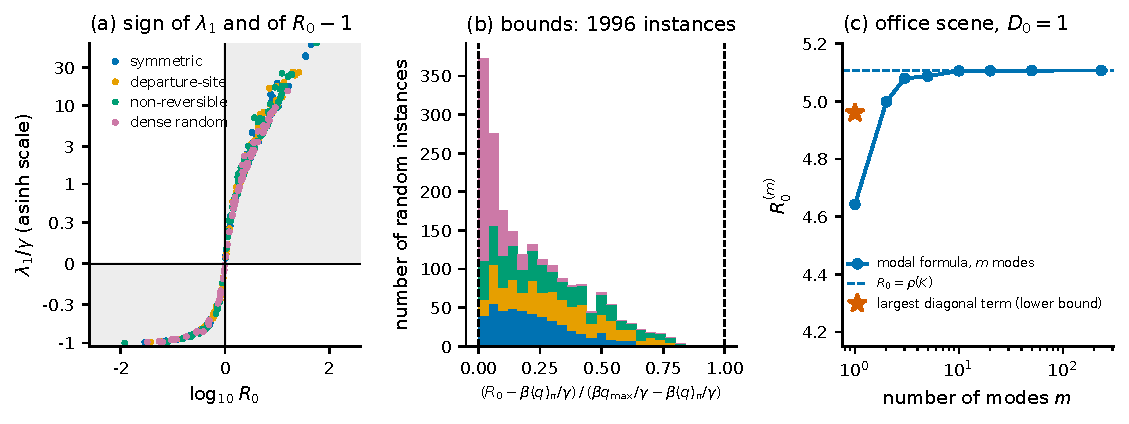
\includegraphics[width=\textwidth]{fig_theorem_checks_en}
\caption{Numerical checks of Section~\ref{M-s3_r0:sec}. (a)~Growth rate $\lamone/\gamma$ against $\Rz$ for the
400 random instances of the threshold test, by generator family; all points lie in the two quadrants allowed
by Theorem~\ref{M-s3_r0:thm:ngm}(c). (b)~Position of $\Rz$ between the lower bound $\beta\qmean/\gamma$ (0) and
the upper bound $\beta\qmax/\gamma$ (1) of Theorem~\ref{M-s3_r0:thm:bounds} for the 1{,}996 of the 2{,}000 instances
in which $q$ is not constant (stacked by family, colours as in (a)). (c)~Office scene, $\Dz=1\cellday$,
$\beta=0.5\perday$, $\gamma=0.14\perday$: largest eigenvalue of the leading block of the modal matrix of
Corollary~\ref{s3_r0:cor:modal} against the number $m$ of modes retained, which rises from $\beta\langle q\rangle/\gamma=4.643$ to $\Rz=5.107$ (dashed); the star is the
largest diagonal term, $4.961$, which is a lower bound (Corollary~\ref{s3_r0:cor:modal}).}
% src: data/bsc_theory/T1_points.npy, T2_positions.npy (1996 rows:
%      data/appA_numerics_checks.json: derived/theorems/T2_nonconstant_q);
%      data/plan_theory_checks.json: office/galerkin_R0_by_modes, office/diagonal_modal_max;
%      figure script code/plan_fig_theory.py (fig_theorem_checks)
\label{appA_numerics:fig:checks}
\end{figure}

The table also shows why symmetric rates are assumed in Theorem~\ref{M-s3_r0:thm:edges}: under the
departure-site rule, tripling the mobility of one cell raised $\Rz$ in 201, lowered it in 98 and left it unchanged (to $10^{-10}$) in one of 300
instances.
% src: data/bsc_theory/verify_theorems.json: T3p (departure_up, departure_down)

\subsection{Re-implementation and searches for counter-examples}
\label{appA_numerics:sec:adversarial}

The second set of programs has its own generators and eigen-solvers and other seeds. It repeated the tests on
600 instances for the threshold (residual $2.1\times10^{-14}$, 0 sign failures), 3{,}000 for the bounds
(violation $9\times10^{-16}$), 400 instances and 49 mobility values for the monotone decrease (no increase),
1{,}800 zones (no violation) and 1{,}200 edge changes ($1.4\times10^{-14}$), with the same conclusions for the
leaky room and the hotspot maps.
% src: code/bsc_theory/verify/v1_theorems.log, v1_part2.log; data/checks/theory.json: threshold_test (600, 2.1e-14, 0),
%      bounds_test (3000, 9e-16), monotone_decrease_test (400, 49), zone_bound_test (1800), edge_monotonicity_test
%      (1200, 1.4e-14); notes/VERIFICATION.md: Section 4.1, theory (item 1, item 3, item 4, item 6, item 7, item 9, item 11)
(One check of the absorbing limit first stopped on a floating-point tolerance at exit rate $10^{9}$ and passed
when repeated with $10^{6}$.)
% src: code/bsc_theory/verify/v1_theorems.log (AssertionError), v1_part2.log (first line)

Random instances rarely come near equality, so an optimiser (Nelder--Mead, random restarts) was used to
\emph{minimise} $\Rz/(\beta\qmean/\gamma)-1$ and to \emph{maximise} $\Rz(D_2)-\Rz(D_1)$, $D_2>D_1$, over
non-reversible dense generators of order 3--5 and over $q$. The first searches reported apparent violations of
$-6\times10^{-2}$ for the lower bound and $+5\times10^{-4}$ for the monotonicity.
% src: code/bsc_theory/verify/v1_theorems.log (adversarial min -6.110e-02; adversarial max 5.201e-04)
Both were numerical artefacts. In the first, the stationary vector had been taken from an ill-conditioned
eigen-solve and the optimiser had pushed the rates over 30 orders of magnitude; with the stationary vector
from a linear solve and rates between $\e^{-12}$ and $\e^{12}$, the minimum over 120 optimised instances is
$-7\times10^{-13}$.
% src: code/bsc_theory/verify/v1b_adv.log (rate range 3.6e-12 .. 1.2e18; robust minimum -6.76e-13)
In the second, the increases occurred at condition numbers of $\Vm$ near $10^{12}$, where a generator
assembled in double precision is no longer exactly conservative. In a new search in which every optimised
instance was evaluated in 60-digit arithmetic \citep{mpmath2023} with a generator whose column sums vanish
exactly, the largest value of $\Rz(D_2)-\Rz(D_1)$ over 80 instances (rates between $\e^{-8}$ and $\e^{8}$) was
$8\times10^{-59}$.
% src: code/bsc_theory/verify/v1c_adv3.log (cond(V) = 2.2e12), v1d_adv3_exact.log (7.97e-59 and 0.0;
%      40 instances each with rates within e^{+-4} and e^{+-8})
We repeated both searches with other seeds and evaluated every optimised instance in 60-digit arithmetic.
For the lower bound, the double-precision minimum over 120 instances was $-5\times10^{-14}$, and the exact
values were all positive, the smallest being $2\times10^{-18}$. For the monotonicity, with rates confined to
$[\e^{-c},\e^{c}]$ for $c=4$, $8$ and $15$ (40 instances each), double precision reported increases
up to $1.2\times10^{-6}$, whereas the exact difference was positive in a single instance, by
$1.5\times10^{-62}$, which is zero at the working precision.
% src: data/appA_numerics_checks.json: adversarial/lower_bound/clip12 (min_float64 = -4.8e-14,
%      min_exact = 1.9e-18, n_exact_negative = 0), adversarial/monotonicity/clip4, clip8, clip15
%      (max_float64 up to 1.15e-6; max_exact 1.46e-62, -1.0e-16, -2.0e-17; n_exact_positive 1, 0, 0)
The practical lesson is one of numerical hygiene: a generator assembled in double precision loses exact
conservation, $\one^{\T}\gen=0$, once the products of mobility scale and hop rates span more than about ten
orders of magnitude, and its stationary vector should be obtained from a linear solve; otherwise the theorems
appear to fail, in the searches above by amounts between $10^{-8}$ and $10^{-2}$. The tests of
Table~\ref{appA_numerics:tab:theorems} use log-normal rates of unit order and mobility scales between
$10^{-4}$ and $10^{4}$ ($10^{\pm9}$ only for the two limits, whose deviations are correspondingly larger).
% src: notes/VERIFICATION.md: Section 4.1, theory, further point 3; magnitudes: the logs cited
%      above (-6.1e-2, -5.5e-8, 5.2e-4, 5.8e-5) and appA_numerics_checks.json: adversarial (5.0e-7, 1.2e-6);
%      ranges: code/bsc_theory/scripts/verify_theorems.py (random_instance, Dgrid, Rinf, Rzero)

\subsection{Nonlinear mean-field model}\label{appA_numerics:sec:nonlinear}

The threshold statement concerns the linearisation, so the full system \eqref{M-s2_model:eq:meanfield} was
integrated as well (LSODA, relative tolerance $10^{-9}$), from a spatially uniform seed of $10^{-6}$ of the
population. These runs used one of the two alternative office layouts of Section~\ref{M-s3_r0:sec} (same zone
fractions as the office scene; $\Rz=5.109$ against $5.107$ at the default parameters) and a $20\times13$
two-zone room, not the canonical scenes, and were not repeated on them.
% src: code/bsc_theory/scripts/nonlinear_check.py (office_O1, two_zone("side"), seed 1e-6, rtol 1e-9);
%      data/plan_theory_checks.json: alternative_layouts/O1/R0_D0_1 = 5.109, office/D0=1/R0 = 5.107
With $\beta$ rescaled so that $\Rz=0.80$ and $0.95$, the prevalence never exceeds the seed and the final
attack fraction is $3.9\times10^{-6}$ and $9.9\times10^{-6}$; for $\Rz=1.05$, $1.20$ and $2.00$ it is
$5.1\,\%$, $19.8\,\%$ and $72.6\,\%$.
% src: data/bsc_theory/nonlinear_check.json: A_threshold (final_attack, peak_prevalence)
In the two-zone room (workspace $q=1.5$ on $69.2\,\%$ of the floor at mobility $0.3\,\Dz$, corridor band
$q=0.5$ at $2\,\Dz$, $\Dz=1\cellday$) with $\beta$ chosen so that the well-mixed estimate
$\beta\langle q\rangle/\gamma$ equals $0.900$, the reproduction number is $\Rz=1.076$ and an outbreak occurs:
the attack fraction is $12.4\,\%$, with $97.2\,\%$ of the infections generated in the workspace, whereas the
same room with $q$ replaced by its mean has no outbreak (attack fraction $1.0\times10^{-5}$).
% src: data/bsc_theory/nonlinear_check.json: B_heterogeneity (well_mixed, R0 = 1.0757,
%      final_attack_heterogeneous = 0.1244, share_of_infections_in_workspace = 0.9725, area_share_workspace = 0.692,
%      final_attack_homogenised = 1.0e-5); layout: code/bsc_theory/scripts/layouts.py (D_TWO, Q_TWO)
The second implementation returned the same values to the digits quoted.
% src: code/bsc_theory/verify/v3_dynamics.log, lines (A) and (B)

\subsection{The simulator}\label{appA_numerics:sec:algorithm}

The individual-based model of Section~\ref{M-s2_model:sec:ibm} is a continuous-time Markov chain and is
simulated without time discretisation by the direct method of \citet{gillespie1976general,gillespie1977exact}
(Fig.~\ref{appA_numerics:fig:algorithm}). The production code is a C~routine called from Python. It keeps,
for every cell $y$, the exposure field $E_y=\sum_{i\ \mathrm{infective}}h(x_i,y)$ and the propensity
$n_S(y)\,E_y$, updates them incrementally at each hop, and recomputes them from scratch after every infection
and recovery and after every 20{,}000 hops, which bounds the accumulation of rounding errors. Every replicate
has its own xoshiro256** stream \citep{blackman2021scrambled} derived from the seed of the batch and the
replicate index.
% src: code/bsc_sim/src/bsc_sim/gillespie.c (upd_site, recompute_inf, hop_since >= 20000, rng_seed)

\begin{figure}[tbp]
\centering
\fbox{\begin{minipage}{0.94\textwidth}\small
\textbf{State.} Cells $x_i\in\cells$ and states $\sigma_i\in\{\mathrm{S},\mathrm{I},\mathrm{R}\}$ of the
$\Npop$ people; time $t$.\\[2pt]
\textbf{Initialisation.} Positions independent and uniform on $\cells$ (the stationary law); person~1 is the
index case, infective at $t=0$, at its own position or in a prescribed or randomly drawn cell (several
initial infectives in test~F of Table~\ref{appA_numerics:tab:simulator}).\\[2pt]
\textbf{Loop,} while at least one person is infective and $t<t_{\max}$:
\begin{enumerate}[leftmargin=1.6em,itemsep=1pt,topsep=2pt]
  \item Compute the total rates of hops, $H=\sum_i\sum_y\hop{x_i}{y}$, of recoveries, $\gamma\,n_I$, and of
        infections, $A=\chi(t)\sum_{i\in\mathrm{I}}\sum_{j\in\mathrm{S}}h(x_i,x_j)$, where $n_I$ is the number of
        infectives, the sums in $A$ run over infective people $i$ and susceptible people $j$, $h$ is the pair
        hazard \eqref{M-s2_model:eq:pairhazard} and $\chi(t)$ the schedule multiplier ($\chi\equiv1$ without
        schedule).
  \item Draw a waiting time $\Delta t$ from the exponential distribution with rate $H+\gamma n_I+A$. If
        $t+\Delta t$ lies beyond the
        end of the current schedule segment, move $t$ to that boundary, switch to the rates of the next
        segment and return to step~1 (exact, because the rates are constant within a segment).
  \item Set $t\leftarrow t+\Delta t$ and choose the type of event with probabilities proportional to
        $H$, $\gamma n_I$, $A$:\\
        \emph{hop}: a person $i$ chosen with probability proportional to its exit rate moves to a neighbour $y$
        chosen with probability proportional to $\hop{x_i}{y}$;\\
        \emph{recovery}: a uniformly chosen infective becomes removed;\\
        \emph{infection}: a pair $(i,j)$ is chosen with probability proportional to $h(x_i,x_j)$; $j$ becomes
        infective, and its infector $i$, generation $g_j=g_i+1$, time and cell are recorded. With the option
        $g_{\max}$, a person of generation above $g_{\max}$ is counted as infected but does not transmit.
\end{enumerate}
\textbf{Output.} Final size, infection tree, numbers of susceptible and infective people on a time grid, and
the exposure $\int_0^{\infty}\chi(t)\sum_{j\ne1}h(x_1,x_j)\,\mathbf{1}[\sigma_1=\mathrm{I}]\,\dd t$ of the index case.
\end{minipage}}
\caption{Exact event-driven simulation of one epidemic. The per-cell rule of Remark~\ref{s5_pair:rem:encounter} is obtained by
replacing the infection rate $A$ by $\sum_y\beta q_y\,n_S(y)\,n_I(y)/n_{\mathrm{tot}}(y)$, with $n_S(y)$,
$n_I(y)$ and $n_{\mathrm{tot}}(y)$ the numbers of susceptible people, of infectives and of all people in cell
$y$.}
% src: code/bsc_sim/src/bsc_sim/refsim.py (reference implementation of exactly these steps),
%      code/bsc_sim/src/bsc_sim/gillespie.c (potential_rate = exposure integrand; mode 1 = per-cell rule)
\label{appA_numerics:fig:algorithm}
\end{figure}

Because the infection tree is recorded, secondary cases are counted and not fitted; with $g_{\max}=0$ only the
index case transmits, which measures $\Rone$ without interference from later cases. The \emph{exposure} of the
index case is the time integral of the rate at which it would infect if everybody within its contact
neighbourhood were susceptible; its expectation for an index case born in cell $x$ is the offspring number
$\noff(x)$ of \eqref{M-s3_r0:eq:offspring}, so that it equals $\Rz$ when $x$ is drawn from the incidence map
$\wvec$. This identity ties the simulator to the next-generation matrix without any approximation.

\subsection{Validation of the simulator}\label{appA_numerics:sec:validation}

Table~\ref{appA_numerics:tab:simulator} lists seven tests; Fig.~\ref{appA_numerics:fig:validation} shows
three of them.

\begin{table}[tbp]
\centering
\caption{Tests of the simulator. $\beta=0.5\perday$, $\gamma=0.14\perday$; scenes with their default
occupancy and $\Dz=1\cellday$ unless stated; $z$ is a difference in units of its standard error.}
\label{appA_numerics:tab:simulator}
\footnotesize
\begin{tabular}{@{}p{0.3cm}p{6.5cm}p{8.3cm}@{}}
\toprule
 & Test & Result\\
\midrule
A & C~routine against a separately written pure-Python implementation of
    Fig.~\ref{appA_numerics:fig:algorithm} (own code and generator); $4\times3$ lattice with one barrier, two
    $q$ zones, two mobility zones, 10 people; $20{,}000$ against $1{,}500$ runs; same-cell kernel, kernel of
    radius one cell, the per-cell rule of Remark~\ref{s5_pair:rem:encounter}, and $g_{\max}=0$ &
    mean final size $6.101$ against $6.065$, $6.776$ against $6.755$, $3.157$ against $3.106$, $3.190$
    against $3.240$; $|z|\le1.31$ for the eight means compared; $\chi^2$ of the final-size histograms $3.6$
    to $10.4$ on 9 degrees of freedom ($p\ge0.32$)\\
% src: data/bsc_sim/01_validation.json: A_c_vs_python; p-values and max |z|:
%      data/appA_numerics_checks.json: derived/A
\addlinespace[3pt]
B & one cell, 40 people: Markovian SIR epidemic with pair hazard $\beta/39$, whose final-size law is computed
    exactly by recursion on the embedded jump chain \citep[cf.][]{andersson2000stochastic}; $40{,}000$ runs &
    mean final size $27.769\pm0.084$ against $27.808$; probability of at most 3 cases $0.2725$ against
    $0.2719$; $\chi^2=39.8$ on 39 degrees of freedom ($p=0.44$); larger samples in the text\\
% src: data/bsc_sim/01_validation.json: B_wellmixed_exact; p-value: appA_numerics_checks.json: derived/B
\addlinespace[3pt]
C & exposure identity; office scene (same-cell kernel) and classroom (1\,m kernel); $40{,}000$ runs for random
    index cells, $10{,}000$ for fixed cells &
    office: index from $\wvec$, $5.055$ ($4.996$--$5.115$) against $\Rz=5.107$; uniform index, $4.681$
    ($4.625$--$4.737$) against $\beta\langle q\rangle/\gamma=4.643$; cells with largest and smallest $\noff(x)$,
    $5.449$ ($5.318$--$5.581$) against $5.335$ and $3.962$ ($3.864$--$4.060$) against $3.995$.
    Classroom: $5.855$ ($5.787$--$5.922$) against $5.866$; $4.697$ ($4.640$--$4.753$) against $4.706$; $6.939$
    ($6.787$--$7.090$) against $6.892$; $3.010$ ($2.936$--$3.084$) against $3.029$. Largest $|z|=1.72$\\
% src: data/bsc_sim/01_validation.json: C_exposure_identity; max |z|: appA_numerics_checks.json: derived/C
\addlinespace[3pt]
D & counted secondary cases with $g_{\max}=0$ and a uniformly placed index case against $\Ronebar$ from the
    exact pair solve \eqref{M-s5_pair:eq:pair}; nine configurations, $20{,}000$ runs each &
    office, $\Dz=0.1$, $1$, $10$, $100$: $0.899$, $2.293$, $3.821$, $4.372$ against $0.895$, $2.266$, $3.793$,
    $4.341$; supermarket $1.985$ against $1.990$; classroom $1.576$ against $1.559$ (same cell) and $2.568$
    against $2.581$ (1\,m); metro $1.517$ against $1.514$ and $5.549$ against $5.584$. All nine values of
    $\Ronebar$ lie inside the 95\,\% intervals; $|z|\le1.52$; differences at most $1.2\,\%$. The mean-field
    values $\beta\langle q\rangle/\gamma$ are $4.643$, $3.263$, $4.706$ and $9.056$\\
% src: data/bsc_sim/01_validation.json: D_pair_theory; summary: appA_numerics_checks.json: derived/D
\addlinespace[3pt]
E & per-cell rule of Remark~\ref{s5_pair:rem:encounter}, 100 people, $20{,}000$ runs &
    secondary cases of the index case $0.690$ ($0.676$--$0.704$) in the office scene and $0.382$
    ($0.372$--$0.392$) in a uniform $20\times20$ room; mean final size $2.6$ and $1.6$ people
    (Remark~\ref{s5_pair:rem:encounter})\\
% src: data/bsc_sim/01_validation.json: test E (per-cell rule)
\addlinespace[3pt]
F & mean-field limit: office scene, $1\,\%$ initially infective; mean prevalence curve against the lattice
    system \eqref{M-s2_model:eq:meanfield} &
    largest absolute difference of the curves $0.423$ ($\Npop=100$, $\Dz=1$; 200 runs), $0.058$
    ($\Npop=1000$, $\Dz=10$; 200 runs), $0.004$ ($\Npop=5000$, $\Dz=100$; 40 runs); final size $0.9898$
    against $0.9900$ in the last case\\
% src: data/bsc_sim/01_validation.json: F_meanfield_limit (max_abs_diff_curve, sim_final_mean, ode_final)
\addlinespace[3pt]
G & schedules, office scene: (i)~three identical segments per day against no schedule, $20{,}000$ runs each;
    (ii)~room occupied during the first third of each day, $40{,}000$ runs &
    (i)~mean final size $23.61$ against $23.69$ people ($|z|=0.31$), secondary cases of the index $1.872$
    against $1.861$ ($|z|=0.57$), fraction of major outbreaks $0.5001$ against $0.4996$; (ii)~exposure $1.631$
    ($1.609$--$1.653$) against $\beta\langle q\rangle\times2.493\ \mathrm{days}=1.620$\\
% src: data/bsc_sim/01_validation.json: G_schedules
\bottomrule
\end{tabular}
\end{table}

\begin{figure}[tbp]
\centering
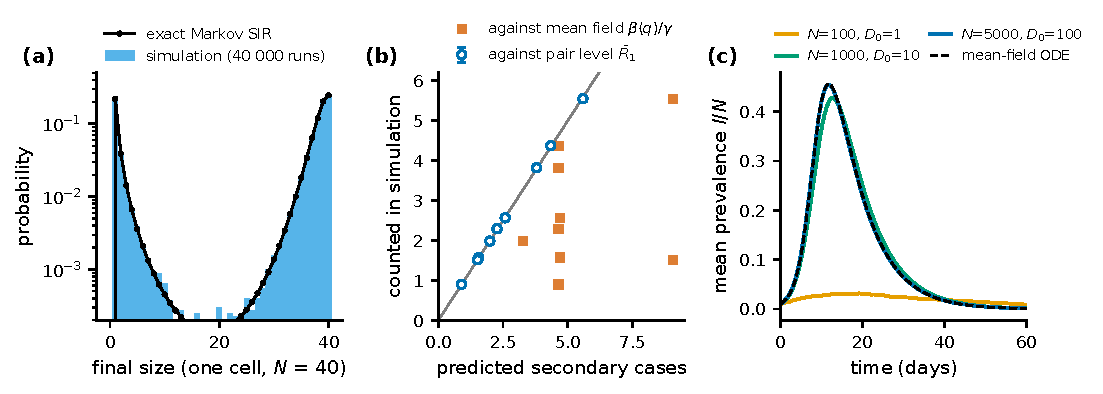
\includegraphics[width=\textwidth]{figA_validation_en}
\caption{Validation of the simulator. (a)~Test~B: final-size distribution of the one-cell model with 40
people, simulation ($40{,}000$ runs) and exact law. (b)~Test~D: counted secondary cases of a uniformly placed
index case ($g_{\max}=0$, $20{,}000$ runs per point; the 95\,\% intervals are about the size of the symbols)
against
$\Ronebar$ from the pair solve (circles) and against the mean-field value
$\beta\langle q\rangle/\gamma$ (squares), for the nine configurations of
Table~\ref{appA_numerics:tab:simulator}. (c)~Test~F: mean prevalence in the office scene with $1\,\%$ initially
infective for three combinations of the number of people $\Npop$ and the mobility scale $\Dz$
(\cdunit{}), and the mean-field solution for $\Dz=100$ (dashed).}
% src: code/bsc_sim/experiments/21_figures_more.py (fig_validation) <- data/bsc_sim/01_validation.json,
%      01_B_finalsize.npz, 01_F_curves.npz
\label{appA_numerics:fig:validation}
\end{figure}

Tests~A to~D and~G establish that the code simulates the stated model; test~C in addition shows that the
simulator and $\ngm$ describe the same model, so that the gap between $\Ronebar$ and the mean-field value
in test~D (ratios $0.17$ to $0.93$) is a property of discrete individuals and not of the code. Test~F shows the
convergence to the mean-field model, and how far the default parameters are from it.
% src: data/appA_numerics_checks.json: derived/D/rows/ratio_to_meanfield (0.167 ... 0.935)

\paragraph{Second simulator.} The checking programs contain a separate exact simulator: it recomputes all
rates from scratch at every event, selects an infection as an (infective, kernel cell) pair, uses another
random-number generator, and has its own scene parser, next-generation matrix and pair solver.
% src: code/bsc_sim/verify/vsim.c (header), vlib.py; notes/VERIFICATION.md: Section 4.2, simulations (item 1)
On the lattice of test~A it gives $2.1818\pm0.0045$ counted secondary cases against $2.1782$ from its pair
solve (same-cell kernel; $200{,}000$ runs), $2.5138\pm0.0050$ against $2.5163$ (radius-one kernel), and
exposures $4.419\pm0.012$ and $4.425\pm0.011$ against $4.416$.
% src: code/bsc_sim/verify/v02_simcheck.json: small_rad0.0, small_rad1.0, small_expo0.0, small_expo1.0
In square rooms of side 4 to 20 with $D=0.51$, $1$ and $10\cellday$ its counts agree with its pair solve
within $1.65$ standard errors in seven configurations ($60{,}000$ to $200{,}000$ runs each).
% src: code/bsc_sim/verify/v04_finite.json, v04.log; max |z|: appA_numerics_checks.json: derived/check_v04
Re-run for this section on the office scene, it gives an exposure of $4.627\pm0.009$ for a uniform index case
against $4.643$ ($400{,}000$ runs; $z=-1.7$) and $5.105\pm0.014$ for an index case drawn from $\wvec$ against
$\Rz=5.107$ ($200{,}000$ runs).
% src: data/appA_numerics_checks.json: simulator/office_exposure (uniform_index, perron_index)
In about 25 configurations in all the two simulators agree within sampling error, the largest differences
being $1.6$ to $2.3$ standard errors (outbreak probability and peak day in the metro scene, outbreak
probability in the office at $\Dz=10$), and the stored results that were re-run from their seeds were
reproduced bit for bit. Two items were not re-simulated with the second simulator: the scene results at $\Dz=100$
and the run with $5{,}000$ people of test~F, which was only repeated with the same code and another seed
(largest difference $0.007$).
% src: data/checks/simulation.json: second_simulator (about 25 configurations; 1.6, 2.3), first_analysis_test_F (0.007),
%      not_resimulated_with_second_simulator; notes/VERIFICATION.md: Section 4.2, simulations (item 1, item 4, summary)

\paragraph{The exact final-size law with larger samples.} On the one-cell model the second simulator's own
batch of $40{,}000$ runs gave a mean of $27.872\pm0.084$ and $\chi^2=55.7$ on 39 degrees of freedom
($p=0.040$).
% src: code/bsc_sim/verify/v02_simcheck.json: wellmixed; p-value: appA_numerics_checks.json: derived/check_v02
To find out whether this signals a defect, both simulators were run $4\times10^{6}$ times. The second
simulator then agreed with the exact law (mean $27.812\pm0.008$, $\chi^2=45.4$, $p=0.22$), but the mean of
the production code lay $2.6$ standard errors above the exact value ($27.830\pm0.008$; $\chi^2=30.2$,
$p=0.84$). A further $2\times10^{7}$ runs of each with other seeds gave $27.805\pm0.004$ ($0.7$ standard errors
below; $\chi^2=44.2$, $p=0.26$) for the production code and $27.811\pm0.004$ ($\chi^2=32.2$, $p=0.77$) for the
second simulator. Over all $2.4\times10^{7}$ runs the means are $27.8096\pm0.0034$ and $27.8110\pm0.0034$
against the exact $27.8082$, with $\chi^2=34.1$ ($p=0.69$) and $37.4$ ($p=0.54$). We conclude that both
deviations were sampling fluctuations; they are reported because they were observed.
% src: data/appA_numerics_checks.json: simulator/wellmixed (article and second: stage1/pooled,
%      stage2/pooled, combined; exact_mean = 27.8082)

\subsection{Reproducibility}\label{appA_numerics:sec:repro}

All random numbers come from generators with fixed seeds that are set in the source of each script (for
example $20261001$ for the theorem tests and one seed per validation test), so that re-running a script
reproduces its stored output.
% src: code/bsc_theory/scripts/verify_theorems.py; code/bsc_theory/verify/v1_theorems.py, v1b_adv.py,
%      v1d_adv3_exact.py; code/bsc_sim/experiments/01_validate.py; code/appA_numerics_checks.py
The computations used Python~3.14.6 with NumPy~2.5.3 \citep{harris2020array}, SciPy~1.18.1
\citep{virtanen2020scipy}, Matplotlib~3.11.2 \citep{hunter2007matplotlib} and mpmath~1.3.0
\citep{mpmath2023}; the C~routines were compiled with Apple clang~21 at optimisation level~2.
% src: data/appA_numerics_checks.json: derived/environment
On one core of a laptop (Apple M4~Pro) the production simulator needs $0.5$\,ms for one epidemic in the
office scene ($100$ people, $\Dz=1\cellday$, about $5{,}900$ events), against $1.8$\,s for the pure-Python
reference implementation; the validation tests take about 8~minutes, the theorem tests 38~seconds, the script
of this section about 9~minutes, and all simulation experiments of the article 3 to 4~hours, with a peak
memory use below $1.5$\,GB.
% src: data/appA_numerics_checks.json: derived/timing (c_core_ms_per_office_epidemic = 0.51,
%      events_per_office_epidemic = 5949, python_reference_s_per_office_epidemic = 1.79), adversarial/runtime_s,
%      simulator/runtime_s; reproduce.md, Section 2.2 (8 min; 3-4 h; 1.5 GB)
In the repository \citep{zhouyi2026code}, \texttt{code} holds the simulator (the C~routine, its Python front
end, the reference implementation and the deterministic solvers), one script per experiment, the theorem
tests, the checking programs and one script per section of this article; \texttt{data} holds the output of
every script, mostly as JSON files, which are the primary record from which all tables and figures are
generated; and \texttt{reproduce.md} gives the command for each of them.


{\small\setlength{\bibsep}{1pt plus 0.5pt}
\bibliographystyle{plainnat}
\bibliography{refs}}

\end{document}
